% ============================================================
%  يُترجَم بـ XeLaTeX  (في Overleaf: Menu → Compiler → XeLaTeX)
%  الخط: Amiri (متوفر في Overleaf، أو حمّله من github.com/aliftype/amiri)
% ============================================================
\documentclass[12pt,a4paper]{article}
\usepackage[a4paper,margin=1.7cm,top=2.3cm,bottom=2.9cm,headheight=15pt,footskip=1.5cm]{geometry}
\usepackage{amsmath,amssymb}
\usepackage{icomma}
\usepackage[english,bidi=default,layout=lists]{babel}
\babelprovide[import,main]{arabic}
\babelfont{rm}[Scale=1.08]{Amiri}
\babelfont{sf}[Scale=1.08]{Amiri}
\usepackage[most]{tcolorbox}
\usepackage{tikz}
\usetikzlibrary{arrows.meta,calc,shadings}
\usepackage{array}
\usepackage{colortbl}
\usepackage{fancyhdr}
\usepackage{titlesec}
\usepackage{enumitem}
\usepackage{collcell}
\usepackage{needspace}
\usepackage{etoolbox}
\newcolumntype{C}{>{\collectcell\ar}c<{\endcollectcell}}
\pretocmd{\section}{\Needspace{15\baselineskip}}{}{}
\pretocmd{\subsection}{\Needspace{11\baselineskip}}{}{}

\definecolor{cDef}{HTML}{1F4E9C}
\definecolor{cThm}{HTML}{B3261E}
\definecolor{cRem}{HTML}{2E7D32}
\definecolor{cEx}{HTML}{C76B00}
\definecolor{cMeth}{HTML}{6A1B9A}
\definecolor{cSol}{HTML}{00695C}
\definecolor{cSec}{HTML}{1F3A68}

\titleformat{\section}{\Large\bfseries\color{cSec}}{\thesection.}{0.6em}{}[{\color{cSec!60}\titlerule[1pt]}]
\titleformat{\subsection}{\large\bfseries\color{cThm!85!black}}{\thesubsection.}{0.5em}{}
\titlespacing*{\section}{0pt}{14pt}{8pt}
\titlespacing*{\subsection}{0pt}{10pt}{5pt}
\setlength{\parindent}{0pt}
\setlength{\parskip}{4pt}
\setlist{itemsep=2pt,topsep=3pt}

\newtcolorbox{arbox}[3][]{enhanced,
  colback=#2!5,colframe=#2!80!black,arc=2mm,boxrule=0.8pt,
  left=6pt,right=6pt,top=8pt,bottom=5pt,
  fonttitle=\bfseries,coltitle=white,
  title={\foreignlanguage{arabic}{#3}},
  attach boxed title to top right={xshift=-5mm,yshift=-3mm},
  boxed title style={colback=#2!80!black,arc=1.5mm,boxrule=0pt},
  before upper={\selectlanguage{arabic}},
  before skip=8pt,after skip=8pt,breakable,#1}
\newenvironment{BOX}[2]{\begin{otherlanguage}{english}\begin{arbox}{#1}{#2}}{\end{arbox}\end{otherlanguage}}
\newenvironment{tarif}[1][تعريف]{\begin{BOX}{cDef}{#1}}{\end{BOX}}
\newenvironment{khassia}[1][خاصية]{\begin{BOX}{cThm}{#1}}{\end{BOX}}
\newenvironment{molahada}[1][ملاحظة]{\begin{BOX}{cRem}{#1}}{\end{BOX}}
\newenvironment{mithal}[1][مثال]{\begin{BOX}{cEx}{#1}}{\end{BOX}}
\newenvironment{tariqa}[1][طريقة]{\begin{BOX}{cMeth}{#1}}{\end{BOX}}

\newcounter{exo}
\newenvironment{tamrin}[1]{\stepcounter{exo}\begin{BOX}{cSec}{التمرين \theexo: #1}}{\end{BOX}}
\newenvironment{hal}{\Needspace{12\baselineskip}\begin{otherlanguage}{english}\begin{arbox}[breakable]{cSol}{حل التمرين \theexo}}{\end{arbox}\end{otherlanguage}}

\newenvironment{LTR}{\begin{otherlanguage}{english}}{\end{otherlanguage}}
\newcommand{\ar}[1]{\foreignlanguage{arabic}{#1}}

\renewcommand{\dots}{\mathinner{\ldotp\ldotp\ldotp}}
\renewcommand{\ldots}{\mathinner{\ldotp\ldotp\ldotp}}
\renewcommand{\cdots}{\mathinner{\cdotp\cdotp\cdotp}}
\newcommand{\N}{\mathbb{N}}
\newcommand{\Z}{\mathbb{Z}}
\newcommand{\D}{\mathbb{D}}
\newcommand{\Q}{\mathbb{Q}}
\newcommand{\R}{\mathbb{R}}
\newcommand{\pgcd}{\operatorname{PGCD}}
\newcommand{\ppcm}{\operatorname{PPCM}}

% \NLseg{a}{b}{[}{]} ; \NLright{a}{[} ; \NLleft{b}{]}  (interval on a number line)
\newcommand{\NLseg}[4]{\begin{LTR}\begin{tikzpicture}[baseline=-0.6ex]
 \draw[-{Stealth[length=2mm]},gray!70](0,0)--(3.4,0);
 \draw[line width=2pt,cThm!80!black](0.7,0)--(2.7,0);
 \node[cThm!80!black,font=\LARGE] at (0.7,0){$#3$};
 \node[cThm!80!black,font=\LARGE] at (2.7,0){$#4$};
 \node[below=3pt,font=\footnotesize] at (0.7,0){$#1$};
 \node[below=3pt,font=\footnotesize] at (2.7,0){$#2$};
\end{tikzpicture}\end{LTR}}
\newcommand{\NLright}[2]{\begin{LTR}\begin{tikzpicture}[baseline=-0.6ex]
 \draw[-{Stealth[length=2mm]},gray!70](0,0)--(3.4,0);
 \draw[line width=2pt,cThm!80!black](1.3,0)--(3.3,0);
 \node[cThm!80!black,font=\LARGE] at (1.3,0){$#2$};
 \node[below=3pt,font=\footnotesize] at (1.3,0){$#1$};
\end{tikzpicture}\end{LTR}}
\newcommand{\NLleft}[2]{\begin{LTR}\begin{tikzpicture}[baseline=-0.6ex]
 \draw[-{Stealth[length=2mm]},gray!70](0,0)--(3.4,0);
 \draw[line width=2pt,cThm!80!black](0.05,0)--(2.1,0);
 \node[cThm!80!black,font=\LARGE] at (2.1,0){$#2$};
 \node[below=3pt,font=\footnotesize] at (2.1,0){$#1$};
\end{tikzpicture}\end{LTR}}

% ---------- social-media icons (pure TikZ) ----------
\definecolor{cFB}{HTML}{1877F2}
\definecolor{cTG}{HTML}{229ED9}
\definecolor{cIG1}{HTML}{FEDA75}
\definecolor{cIG2}{HTML}{D62976}
\definecolor{cIG3}{HTML}{4F5BD5}
\newcommand{\fbicon}{\begin{LTR}\begin{tikzpicture}[baseline=-0.75ex,x=1em,y=1em]
 \fill[cFB] (0,0) circle (0.55);
 \node[white,inner sep=0,font=\usefont{TU}{lmss}{bx}{n}\small] at (0.04,-0.02) {f};
\end{tikzpicture}\end{LTR}}
\newcommand{\igicon}{\begin{LTR}
\begin{tikzpicture}[baseline=-0.75ex,x=1em,y=1em]
 \shade[lower left=cIG1,lower right=cIG2,upper left=cIG2,upper right=cIG3,rounded corners=0.28em] (-0.55,-0.55) rectangle (0.55,0.55);
 \draw[white,line width=0.09em,rounded corners=0.18em] (-0.36,-0.36) rectangle (0.36,0.36);
 \draw[white,line width=0.09em] (0,0) circle (0.17);
 \fill[white] (0.22,0.22) circle (0.05);
\end{tikzpicture}\end{LTR}}
\newcommand{\tgicon}{\begin{LTR}
\begin{tikzpicture}[baseline=-0.75ex,x=1em,y=1em]
 \fill[cTG] (0,0) circle (0.55);
 \fill[white] (-0.33,0.0) -- (0.32,0.27) -- (0.2,-0.3) -- (0.0,-0.15) -- (-0.08,-0.28) -- (-0.08,-0.08) -- cycle;
 \fill[cTG!70!black] (-0.08,-0.08) -- (0.25,0.2) -- (0.0,-0.15) -- (-0.08,-0.28) -- cycle;
\end{tikzpicture}\end{LTR}}
% page number: black box, white two-digit number, at the right of the social row
\newcommand{\PageBox}{\begin{LTR}\tikz[baseline=(p.base)]\node[fill=black,text=white,inner sep=2.5pt,minimum width=1.6em,minimum height=1.3em,font=\usefont{TU}{lmss}{bx}{n}\small](p){\ifnum\value{page}<10 0\fi\arabic{page}};\end{LTR}}
% visual left-to-right order: Telegram | Instagram | Facebook | page box
\newcommand{\SocialRow}{\begin{otherlanguage}{english}%
 \ar{\textbf{الأستاذ سوايسية هشام للرياضيات}}\ \tgicon\hfill
 \textbf{prof\_hicham\_math}\ \igicon\hfill
 \ar{\textbf{الأستاذ سوايسية هشام للرياضيات}}\ \fbicon\hspace{2.2em}\PageBox\end{otherlanguage}}

\pagestyle{fancy}
\fancyhf{}
\renewcommand{\headrulewidth}{0.6pt}
\renewcommand{\footrulewidth}{0.4pt}
% \SetHeader{right head: document title}{left head: level -- stream}
\newcommand{\SetHeader}[2]{%
 \fancyhead[C]{\parbox{\textwidth}{\ar{#1\hfill #2}}}%
 \fancyfoot[C]{\parbox{\textwidth}{\small\SocialRow}}}
\usepackage{tkz-tab}
\usepackage{multicol}
% variation / sign table (LTR)
\newenvironment{TAB}{\par\begin{center}\begin{LTR}\begin{tikzpicture}[scale=0.95,every node/.style={font=\small}]}{\end{tikzpicture}\end{LTR}\end{center}}
% grid + axes, clipped: \begin{GR}{xmin}{xmax}{ymin}{ymax}{unit cm}
\newenvironment{GR}[5]{\par\begin{center}\begin{LTR}\begin{tikzpicture}[x=#5cm,y=#5cm,font=\footnotesize]
 \draw[gray!25,very thin] (#1,#3) grid (#2,#4);
 \draw[-{Stealth[length=2mm]}] (#1,0)--(#2+0.3,0) node[below left]{$x$};
 \draw[-{Stealth[length=2mm]}] (0,#3)--(0,#4+0.3) node[below left]{$y$};
 \node[below left] at (0,0){$O$};
 \begin{scope}\clip (#1,#3) rectangle (#2,#4);}
{\end{scope}\end{tikzpicture}\end{LTR}\end{center}}
\newcommand{\Ticks}[2]{\foreach \t in {#1} \node[below,font=\scriptsize] at (\t,0){$\t$}; \foreach \t in {#2} \node[left,font=\scriptsize] at (0,\t){$\t$};}
\newcommand{\bx}[1]{\ensuremath{\colorbox{cDef!12}{$\displaystyle #1$}}}
\newcommand{\TwoCol}[4]{\par\begin{LTR}\noindent\begin{minipage}[t]{#1\textwidth}\selectlanguage{arabic}#2\end{minipage}\hfill\begin{minipage}[t]{#3\textwidth}\selectlanguage{arabic}#4\end{minipage}\end{LTR}\par}
\newcommand{\RL}[4]{\TwoCol{#3}{#4}{#1}{#2}}  % \RL{w1}{right content}{w2}{left content}
\newcommand{\ok}{$\textcolor{cRem}{\checkmark}$}
\newcommand{\limn}{\displaystyle\lim_{n\to+\infty}}
% sub-questions, each on its own line
\newenvironment{sq}{\begin{itemize}[leftmargin=2.4em,itemsep=3pt]}{\end{itemize}}
\newcommand{\qa}{\item[(أ)]}\newcommand{\qb}{\item[(ب)]}\newcommand{\qc}{\item[(جـ)]}\newcommand{\qd}{\item[(د)]}\newcommand{\qe}{\item[(هـ)]}
\newcommand{\pa}{\par\smallskip\textbf{(أ)} }\newcommand{\pb}{\par\smallskip\textbf{(ب)} }\newcommand{\pc}{\par\smallskip\textbf{(جـ)} }\newcommand{\pd}{\par\smallskip\textbf{(د)} }\newcommand{\pe}{\par\smallskip\textbf{(هـ)} }
\newcommand{\QQ}[1]{\par\smallskip\textbf{#1.} }
\newenvironment{tmr}{\stepcounter{exo}\begin{BOX}{cSec}{تمرين محلول \theexo}}{\end{BOX}}
\newcommand{\ABC}[3]{\\[2pt]\begin{tabular}{p{0.28\textwidth}p{0.28\textwidth}p{0.28\textwidth}}(جـ) \ #3 & (ب) \ #2 & (أ) \ #1\end{tabular}}
\pretocmd{\section}{\Needspace{24\baselineskip}}{}{}
\newtcbox{\bxtbox}{on line,colback=cDef!12,colframe=cDef!12,boxrule=0pt,arc=1pt,boxsep=0pt,left=2pt,right=2pt,top=1pt,bottom=1pt}
\newcommand{\bxt}[1]{\foreignlanguage{english}{\bxtbox{\ar{#1}}}}
\SetHeader{\small\bfseries\color{cSec}تمارين البكالوريا: المتتاليات العددية}{\small\color{cSec}السنة الثالثة ثانوي -- الشعب العلمية}
\begin{document}
\begin{LTR}
\begin{tcolorbox}[enhanced,colback=cSec,colframe=cSec,arc=3mm,halign=center,boxrule=0pt,top=12pt,bottom=12pt,before upper={\selectlanguage{arabic}}]
{\color{white}\fontsize{26}{32}\selectfont\bfseries تمارين البكالوريا في المتتاليات العددية}\\[8pt]
{\color{white}\large مع الحلول المفصلة خطوة بخطوة -- حتى دورة 2026}\\[5pt]
{\color{white}\large علوم تجريبية -- تقني رياضي -- رياضيات}
\end{tcolorbox}
\end{LTR}
\section{تمارين البكالوريا -- شعبة علوم تجريبية}
% ===================== بكالوريا 2026 -- علوم تجريبية =====================
\begin{tamrin}{بكالوريا 2026 -- الموضوع الأول -- علوم تجريبية}
\QQ{1} ادرس اتجاه تغيّر الدالة $f$ المعرّفة على المجال $]-2;+\infty[$ بـ: $f(x)=\dfrac{4x}{x+2}$.

\QQ{2} $(u_n)$ المتتالية العددية المعرّفة بـ: $u_0=4$ ومن أجل كلّ عدد طبيعي $n$: $u_{n+1}=f(u_n)$.
\begin{sq}
\qa احسب $u_1$ و$u_2$ ثمّ خمّن اتجاه تغيّر المتتالية $(u_n)$.
\qb برهن بالتراجع أنّه: من أجل كلّ عدد طبيعي $n$، $u_n>2$.
\qc ادرس اتجاه تغيّر المتتالية $(u_n)$.
\end{sq}

\QQ{3} $(v_n)$ المتتالية العددية المعرّفة على $\N$ بـ: $v_n=\dfrac{u_n-2}{u_n}$.
\begin{sq}
\qa أثبت أنّ المتتالية $(v_n)$ هندسية أساسها $\dfrac12$، يُطلب كتابة $v_n$ بدلالة $n$.
\qb عبّر عن $u_n$ بدلالة $n$ ثمّ احسب نهاية المتتالية $(u_n)$.
\end{sq}

\QQ{4} نضع: من أجل كلّ $n$ من $\N$: $S_n=v_0+v_1+\cdots+v_n$ و $T_n=\dfrac{1}{u_0}+\dfrac{1}{u_1}+\cdots+\dfrac{1}{u_n}$.

-- احسب $S_n$ بدلالة $n$ ثمّ استنتج أنّ: $T_n=\dfrac12 n+\left(\dfrac12\right)^{n+2}$.
\end{tamrin}

\begin{hal}
\QQ{1} \textbf{اتجاه تغيّر $f$:} الدالة $f$ ناطقة معرّفة وقابلة للاشتقاق على $]-2;+\infty[$، ومن أجل كلّ $x$ من هذا المجال:
\[
f'(x)=\frac{4(x+2)-4x\times 1}{(x+2)^2}=\frac{8}{(x+2)^2}.
\]
بما أنّ $8>0$ و$(x+2)^2>0$، فإنّ $f'(x)>0$، إذن \bxt{$f$ متزايدة تمامًا على $]-2;+\infty[$}.

\QQ{2}
\pa $u_1=f(u_0)=f(4)=\dfrac{16}{6}$ أي \bx{u_1=\frac83}، و $u_2=f\!\left(\dfrac83\right)=\dfrac{\frac{32}{3}}{\frac{14}{3}}$ أي \bx{u_2=\frac{16}{7}}.

لدينا $u_0=4$، $u_1\approx 2{,}67$، $u_2\approx 2{,}29$، أي $u_0>u_1>u_2$، نخمّن أنّ \bxt{المتتالية $(u_n)$ متناقصة تمامًا}.

\pb \textbf{البرهان بالتراجع} على الخاصية $P(n)$: «$u_n>2$».
\begin{itemize}
\item \textbf{التحقق:} من أجل $n=0$: $u_0=4>2$، إذن $P(0)$ صحيحة.
\item \textbf{الوراثة:} نفرض أنّ $P(n)$ صحيحة من أجل عدد طبيعي $n$، أي $u_n>2$، ونبرهن أنّ $P(n+1)$ صحيحة، أي $u_{n+1}>2$.

بما أنّ $u_n>2$ و$f$ متزايدة تمامًا على $]-2;+\infty[$ (الذي يحوي $2$ و$u_n$)، فإنّ $f(u_n)>f(2)$، و$f(2)=\dfrac{8}{4}=2$، إذن $u_{n+1}>2$.

(طريقة أخرى: $u_{n+1}-2=\dfrac{4u_n-2u_n-4}{u_n+2}=\dfrac{2(u_n-2)}{u_n+2}>0$ لأنّ $u_n-2>0$ و$u_n+2>0$.)
\item \textbf{الخلاصة:} حسب مبدأ الاستدلال بالتراجع، \bxt{من أجل كلّ عدد طبيعي $n$: $u_n>2$}.
\end{itemize}

\pc من أجل كلّ عدد طبيعي $n$:
\[
u_{n+1}-u_n=\frac{4u_n}{u_n+2}-u_n=\frac{4u_n-u_n^2-2u_n}{u_n+2}=\frac{u_n(2-u_n)}{u_n+2}.
\]
بما أنّ $u_n>2$ فإنّ: $u_n>0$ و$2-u_n<0$ و$u_n+2>0$، إذن $u_{n+1}-u_n<0$، ومنه \bxt{المتتالية $(u_n)$ متناقصة تمامًا} (وهو ما يؤكّد التخمين).

\QQ{3}
\pa $v_n$ معرّف لأنّ $u_n>2$ أي $u_n\neq 0$. من أجل كلّ عدد طبيعي $n$:
\[
v_{n+1}=\frac{u_{n+1}-2}{u_{n+1}}
=\frac{\dfrac{2(u_n-2)}{u_n+2}}{\dfrac{4u_n}{u_n+2}}
=\frac{2(u_n-2)}{4u_n}=\frac12\times\frac{u_n-2}{u_n}=\frac12\,v_n .
\]
إذن $(v_n)$ متتالية هندسية أساسها $q=\dfrac12$ وحدّها الأول $v_0=\dfrac{u_0-2}{u_0}=\dfrac{2}{4}=\dfrac12$.

ومنه: $v_n=v_0\times q^n=\dfrac12\left(\dfrac12\right)^n$ أي \bx{v_n=\left(\frac12\right)^{n+1}}.

\pb من $v_n=\dfrac{u_n-2}{u_n}=1-\dfrac{2}{u_n}$ نجد $\dfrac{2}{u_n}=1-v_n$، و$1-v_n\neq0$ (لأنّ $0<v_n\leq\frac12$)، إذن:
\[
\bx{u_n=\frac{2}{1-v_n}=\frac{2}{1-\left(\frac12\right)^{n+1}}}
\]
لدينا $-1<\dfrac12<1$ إذن $\limn\left(\dfrac12\right)^{n+1}=0$، ومنه \bx{\lim_{n\to+\infty}u_n=\frac{2}{1-0}=2}.

\QQ{4} $S_n$ مجموع $n+1$ حدًّا متتابعًا من المتتالية الهندسية $(v_n)$:
\[
S_n=v_0\times\frac{1-q^{n+1}}{1-q}=\frac12\times\frac{1-\left(\frac12\right)^{n+1}}{\frac12}
\]
إذن \bx{S_n=1-\left(\frac12\right)^{n+1}}.
من السؤال السابق: $\dfrac{1}{u_n}=\dfrac{1-v_n}{2}=\dfrac12-\dfrac12 v_n$، ومنه:
\begin{align*}
T_n&=\sum_{k=0}^{n}\frac{1}{u_k}=\sum_{k=0}^{n}\left(\frac12-\frac12 v_k\right)=\frac12(n+1)-\frac12 S_n\\
&=\frac12(n+1)-\frac12\left(1-\left(\frac12\right)^{n+1}\right)=\frac12 n+\frac12-\frac12+\left(\frac12\right)^{n+2}.
\end{align*}
إذن \bx{T_n=\frac12 n+\left(\frac12\right)^{n+2}}.
\end{hal}

% -------------------------------------------------------------------
\begin{tamrin}{بكالوريا 2026 -- الموضوع الثاني -- علوم تجريبية}
$f$ الدالة المعرّفة على $\left]-\infty;\dfrac32\right[$ بـ: $f(x)=\dfrac{-6x+2}{2x-3}$، و$(C_f)$ تمثيلها البياني في المستوي المنسوب إلى المعلم المتعامد والمتجانس $(O;\vec i,\vec j)$، و$(\Delta)$ المستقيم ذو المعادلة $y=x$ (الشكل).

$(u_n)$ المتتالية العددية المعرّفة بـ: $u_0=0$ ومن أجل كلّ عدد طبيعي $n$: $u_{n+1}=f(u_n)$.

\begin{GR}{-4}{2}{-3}{3}{0.85}
\Ticks{-4,-3,-2,-1,1,2}{-3,-2,-1,1,2,3}
\draw[dashed,thick,gray] (1.5,-3)--(1.5,3);
\draw[thick,cDef] plot[domain=-4:2,samples=2] (\x,\x);
\draw[very thick,cThm,domain=-4:1.36,samples=200] plot (\x,{(-6*\x+2)/(2*\x-3)});
\node[cDef] at (-2.6,-1.6){$(\Delta)$};
\node[cThm] at (-0.75,-1.3){$(C_f)$};
\end{GR}

\QQ{1} بقراءة بيانية، حدّد اتجاه تغيّر الدالة $f$ وبرّر أنّه: من أجل كلّ $x$ من $[-2;0]$، $f(x)-x\leq 0$.

\QQ{2}
\begin{sq}
\qa انقل الشكل على ورقة الإجابة ثمّ مثّل على حامل محور الفواصل الحدود: $u_0$، $u_1$، $u_2$ و$u_3$ (دون حسابها مبرزًا خطوط التمثيل).
\qb خمّن اتجاه تغيّر المتتالية $(u_n)$ وتقاربها.
\end{sq}

\QQ{3}
\begin{sq}
\qa برهن بالتراجع أنّه: من أجل كلّ عدد طبيعي $n$، $-2<u_n\leq 0$.
\qb حدّد اتجاه تغيّر المتتالية $(u_n)$.
\end{sq}

\QQ{4} $(v_n)$ المتتالية العددية المعرّفة على $\N$ بـ: $v_n=\dfrac{4+2u_n}{1-2u_n}$.
\begin{sq}
\qa أثبت أنّ المتتالية $(v_n)$ هندسية أساسها $\dfrac27$، يُطلب كتابة عبارة $v_n$ بدلالة $n$.
\qb عبّر عن $u_n$ بدلالة $n$ ثمّ احسب نهاية المتتالية $(u_n)$.
\end{sq}

\QQ{5} $(w_n)$ المتتالية العددية المعرّفة على $\N$ بـ: $w_n=\ln(v_n)$.
\begin{sq}
\qa بيّن أنّ المتتالية $(w_n)$ حسابية، يُطلب تعيين أساسها وحدّها الأول.
\qb بيّن أنّه: من أجل كلّ $n$ من $\N$، $w_0+w_1+\cdots+w_n=\dfrac12(n+1)\big[(\ln2-\ln7)n+4\ln2\big]$.
\end{sq}
\end{tamrin}

\begin{hal}
\QQ{1} \textbf{بقراءة بيانية:} المنحني $(C_f)$ صاعد على $\left]-\infty;\frac32\right[$، إذن \bxt{$f$ متزايدة تمامًا على $\left]-\infty;\frac32\right[$} وخصوصًا على $[-2;0]$.

على المجال $[-2;0]$ يقع المنحني $(C_f)$ \textbf{تحت} المستقيم $(\Delta)$، ويتقاطعان في النقطة $A(-2;-2)$، إذن من أجل كلّ $x$ من $[-2;0]$: $f(x)\leq x$ أي \bx{f(x)-x\leq 0}.

\textbf{تأكيد حسابي:} $f'(x)=\dfrac{-6(2x-3)-2(-6x+2)}{(2x-3)^2}=\dfrac{14}{(2x-3)^2}>0$، و
\[
f(x)-x=\frac{-6x+2-2x^2+3x}{2x-3}=\frac{-(2x^2+3x-2)}{2x-3}=\frac{(2x-1)(x+2)}{3-2x}.
\]
من أجل $x\in[-2;0]$: $2x-1<0$، $x+2\geq0$، $3-2x>0$، إذن $f(x)-x\leq0$ (تنعدم عند $x=-2$ فقط).

\QQ{2}
\pa نبدأ من $u_0=0$ على محور الفواصل، نصعد (أو ننزل) عموديًّا إلى $(C_f)$ فنحصل على $u_1=f(u_0)$ على محور التراتيب، ثمّ ننقله إلى محور الفواصل بواسطة المستقيم $(\Delta)$ (أفقيًّا إلى $(\Delta)$ ثمّ عموديًّا إلى محور الفواصل)، ونكرّر:
\begin{GR}{-3}{1}{-3}{1}{1.9}
\Ticks{-3,-2,-1,1}{-3,-2,-1,1}
\draw[thick,cDef] plot[domain=-3:1,samples=2] (\x,\x);
\draw[very thick,cThm,domain=-3:1,samples=150] plot (\x,{(-6*\x+2)/(2*\x-3)});
\draw[cEx,thick,-{Stealth[length=1.6mm]}] (0,0)--(0,-0.6667);
\draw[cEx,thick,-{Stealth[length=1.6mm]}] (0,-0.6667)--(-0.6667,-0.6667);
\draw[cEx,thick,-{Stealth[length=1.6mm]}] (-0.6667,-0.6667)--(-0.6667,-1.3846);
\draw[cEx,thick,-{Stealth[length=1.6mm]}] (-0.6667,-1.3846)--(-1.3846,-1.3846);
\draw[cEx,thick,-{Stealth[length=1.6mm]}] (-1.3846,-1.3846)--(-1.3846,-1.7867);
\draw[cEx,thick,-{Stealth[length=1.6mm]}] (-1.3846,-1.7867)--(-1.7867,-1.7867);
\draw[cEx,dashed] (-0.6667,-0.6667)--(-0.6667,0) (-1.3846,-1.3846)--(-1.3846,0) (-1.7867,-1.7867)--(-1.7867,0);
\foreach \a/\l in {0/0,-0.6667/1,-1.3846/2,-1.7867/3} {\fill[cEx] (\a,0) circle (1.6pt); \node[above,cEx,font=\scriptsize] at (\a,0.05){$u_{\l}$};}
\node[cDef] at (0.8,0.4){$(\Delta)$};
\node[cThm] at (-2.6,-2.55){$(C_f)$};
\node[below right,font=\scriptsize] at (-2,-2){$A$};
\end{GR}
\pb من التمثيل: $u_0>u_1>u_2>u_3$ والحدود تقترب من فاصلة نقطة التقاطع $A(-2;-2)$؛ نخمّن أنّ \bxt{$(u_n)$ متناقصة ومتقاربة نحو $-2$}.

\QQ{3}
\pa \textbf{البرهان بالتراجع} على الخاصية $P(n)$: «$-2<u_n\leq 0$».
\begin{itemize}
\item \textbf{التحقق:} $u_0=0$ و $-2<0\leq0$، إذن $P(0)$ صحيحة.
\item \textbf{الوراثة:} نفرض $-2<u_n\leq0$ ونبرهن $-2<u_{n+1}\leq0$.

بما أنّ $f$ متزايدة تمامًا على $\left]-\infty;\frac32\right[$ فإنّ: $f(-2)<f(u_n)\leq f(0)$، أي $-2<u_{n+1}\leq -\dfrac23$، ومنه $-2<u_{n+1}\leq 0$.
\item \textbf{الخلاصة:} \bxt{من أجل كلّ عدد طبيعي $n$: $-2<u_n\leq0$}.
\end{itemize}

\pb من أجل كلّ عدد طبيعي $n$: $u_{n+1}-u_n=f(u_n)-u_n=\dfrac{(u_n+2)(2u_n-1)}{3-2u_n}$.

بما أنّ $-2<u_n\leq0$: $u_n+2>0$، $2u_n-1<0$، $3-2u_n>0$، إذن $u_{n+1}-u_n<0$ (أو مباشرة من السؤال 1: $u_n\in[-2;0]$ إذن $f(u_n)-u_n\leq0$).

إذن \bxt{المتتالية $(u_n)$ متناقصة تمامًا}.

\QQ{4}
\pa $v_n$ معرّف لأنّ $u_n\leq0$ إذن $1-2u_n\geq1>0$. نحسب أوّلًا:
\[
4+2u_{n+1}=4+\frac{2(-6u_n+2)}{2u_n-3}=\frac{8u_n-12-12u_n+4}{2u_n-3}=\frac{-4(u_n+2)}{2u_n-3},
\]
\[
1-2u_{n+1}=1-\frac{2(-6u_n+2)}{2u_n-3}=\frac{2u_n-3+12u_n-4}{2u_n-3}=\frac{7(2u_n-1)}{2u_n-3}.
\]
ومنه:
\[
v_{n+1}=\frac{-4(u_n+2)}{7(2u_n-1)}=\frac{4(u_n+2)}{7(1-2u_n)}=\frac27\times\frac{2(u_n+2)}{1-2u_n}=\frac27\times\frac{4+2u_n}{1-2u_n}=\frac27\,v_n.
\]
إذن $(v_n)$ متتالية هندسية أساسها $q=\dfrac27$ وحدّها الأول $v_0=\dfrac{4+0}{1-0}=4$، ومنه \bx{v_n=4\left(\frac27\right)^n}.

\pb من $v_n(1-2u_n)=4+2u_n$ نجد $v_n-4=2u_n(1+v_n)$، و$1+v_n>0$، إذن:
\[
\bx{u_n=\frac{v_n-4}{2v_n+2}=\frac{4\left(\frac27\right)^n-4}{8\left(\frac27\right)^n+2}=\frac{2\left(\frac27\right)^n-2}{4\left(\frac27\right)^n+1}}
\]
بما أنّ $-1<\dfrac27<1$ فإنّ $\limn\left(\dfrac27\right)^n=0$، إذن \bx{\lim_{n\to+\infty}u_n=\frac{0-2}{0+1}=-2}.

\QQ{5}
\pa $v_n=4\left(\frac27\right)^n>0$ إذن $w_n$ معرّف و:
\[
w_n=\ln\!\left(4\left(\tfrac27\right)^n\right)=\ln4+n\ln\tfrac27=2\ln2+n(\ln2-\ln7).
\]
إذن $w_{n+1}-w_n=\ln\dfrac27$ (ثابت)، ومنه \bxt{$(w_n)$ حسابية أساسها $r=\ln\frac27=\ln2-\ln7$}
\bxt{وحدّها الأول $w_0=\ln4=2\ln2$}.

\pb مجموع $n+1$ حدًّا متتابعًا من متتالية حسابية:
\begin{align*}
w_0+w_1+\cdots+w_n&=\frac{n+1}{2}\,(w_0+w_n)=\frac{n+1}{2}\big[2\ln2+2\ln2+n(\ln2-\ln7)\big]\\
&=\frac12(n+1)\big[(\ln2-\ln7)n+4\ln2\big].
\end{align*}
\end{hal}
% ===================== علوم تجريبية: 2025 -- 2021 =====================
\begin{tamrin}{بكالوريا 2025 -- الموضوع الأول -- علوم تجريبية}
\QQ{1} $f$ الدالة المعرّفة على $[-1;+\infty[$ بـ: $f(x)=\dfrac{3}{x+2}$، و$(C_f)$ تمثيلها البياني في المستوي المنسوب إلى معلم متعامد ومتجانس $(O;\vec i,\vec j)$، و$(\Delta)$ المستقيم الذي معادلته $y=x$ كما في الشكل أدناه.

\begin{GR}{-1.5}{4.5}{-0.5}{3.5}{1.3}
\Ticks{-1,1,2,3,4}{1,2,3}
\draw[cThm,thick] (-0.5,-0.5)--(3.5,3.5);
\draw[cDef,thick,domain=-1:4.5,samples=80] plot(\x,{3/(\x+2)});
\fill[cDef] (-1,3) circle (1.5pt);
\node[cDef] at (3.6,1.0){$(C_f)$};
\node[cThm] at (2.6,3.2){$(\Delta)$};
\end{GR}

المتتالية العددية $(u_n)$ معرّفة بـ: $u_0=-1$، ومن أجل كل عدد طبيعي $n$: $u_{n+1}=f(u_n)$.
\begin{sq}
\qa أنقل الشكل على ورقة الإجابة ثمّ مثّل على حامل محور الفواصل الحدود $u_0$، $u_1$، $u_2$ و$u_3$.
\qb ضع تخمينا حول اتّجاه تغيّر المتتالية $(u_n)$ وتقاربها.
\end{sq}
\QQ{2} $(v_n)$ المتتالية العددية المعرّفة على $\N$ بـ: $v_n=\dfrac{1-u_n}{3+u_n}$.
\begin{sq}
\qa بيّن أنّ المتتالية $(v_n)$ هندسية أساسها $-\dfrac13$، ثمّ اكتب $v_n$ بدلالة $n$.
\qb استنتج كتابة $u_n$ بدلالة $n$، ثمّ احسب $\limn u_n$.
\end{sq}
\QQ{3} احسب بدلالة $n$ كلًّا من $S_n$ و$T_n$ حيث:
\[S_n=v_0+v_1+\cdots+v_n\qquad;\qquad T_n=\ln|v_0|+\ln|v_1|+\cdots+\ln|v_n|\]
\end{tamrin}

\begin{molahada}
في نسخة المصدر كُتب $u_0=1$ ومجال تعريف $f$ مفتوح عند $-1$. مع $u_0=1$ يكون $v_0=0$ فتصبح $(v_n)$ معدومة ولا يُعرَّف $\ln|v_0|$، والشكل يبدأ تمثيل الحدود من الفاصلة $-1$؛ لذا الصحيح: $u_0=-1$ و$f$ معرّفة على $[-1;+\infty[$.
\end{molahada}

\begin{hal}
\QQ{1}
\pa نمثّل الحدود باستعمال المنحنى $(C_f)$ والمستقيم $(\Delta)$: نبدأ من $u_0=-1$ على محور الفواصل، نصعد شاقوليا إلى $(C_f)$ فنقرأ $u_1=f(u_0)$ على محور التراتيب، ثمّ ننقله إلى محور الفواصل بواسطة $(\Delta)$، وهكذا.

حسابيا (للتحقق): $u_1=\dfrac{3}{-1+2}=3$، $u_2=\dfrac{3}{5}$، $u_3=\dfrac{3}{\frac35+2}=\dfrac{15}{13}\approx 1{,}15$.

\begin{GR}{-1.5}{4.5}{-0.5}{3.5}{1.3}
\Ticks{2,4}{1,2,3}
\draw[cThm,thick] (-0.5,-0.5)--(3.5,3.5);
\draw[cDef,thick,domain=-1:4.5,samples=80] plot(\x,{3/(\x+2)});
\draw[cEx,thick,dashed] (-1,0)--(-1,3)--(3,3)--(3,0.6)--(0.6,0.6)--(0.6,1.1538)--(1.1538,1.1538);
\draw[cEx,dotted] (3,0)--(3,0.6) (0.6,0)--(0.6,0.6) (1.1538,0)--(1.1538,1.1538);
\foreach \a/\l in {-1/u_0,3/u_1,0.6/u_2,1.1538/u_3} {\fill[cEx] (\a,0) circle (1.6pt); \node[below,cEx,font=\scriptsize] at (\a,0){$\l$};}
\node[cDef] at (3.6,1.0){$(C_f)$};
\node[cThm] at (2.6,3.2){$(\Delta)$};
\end{GR}

\pb من الشكل: $u_0<u_1$ بينما $u_2<u_1$، أي أنّ الفرق $u_{n+1}-u_n$ لا يحافظ على إشارة ثابتة، والحدود تتناوب حول فاصلة نقطة تقاطع $(C_f)$ و$(\Delta)$ وتقترب منها.

نحسب هذه الفاصلة: $\dfrac{3}{x+2}=x\iff x^2+2x-3=0\iff (x-1)(x+3)=0$، ومع $x\geqslant -1$ نجد $x=1$.

التخمين: \bxt{المتتالية $(u_n)$ ليست رتيبة، وهي متقاربة نحو $1$.}

\QQ{2}
\pa من أجل كل عدد طبيعي $n$:
\[u_{n+1}=\frac{3}{u_n+2}\ \Rightarrow\ 1-u_{n+1}=\frac{u_n+2-3}{u_n+2}=\frac{u_n-1}{u_n+2}\ ,\quad 3+u_{n+1}=\frac{3u_n+6+3}{u_n+2}=\frac{3(u_n+3)}{u_n+2}\]
إذن:
\[v_{n+1}=\frac{1-u_{n+1}}{3+u_{n+1}}=\frac{u_n-1}{3(u_n+3)}=-\frac13\cdot\frac{1-u_n}{3+u_n}=-\frac13\,v_n\]
ومنه $(v_n)$ هندسية أساسها $q=-\dfrac13$ وحدها الأول $v_0=\dfrac{1-(-1)}{3+(-1)}=1$، إذن:
\[\bx{v_n=\left(-\frac13\right)^n}\]

\pb من $v_n=\dfrac{1-u_n}{3+u_n}$ نجد $v_n(3+u_n)=1-u_n$ أي $u_n(1+v_n)=1-3v_n$، و$1+v_n\neq 0$ لأن $|v_n|\leqslant 1$ و$v_n\neq -1$ (إذ $v_n=-1$ يعطي $1=-3$، وهذا مستحيل)، إذن:
\[\bx{u_n=\frac{1-3v_n}{1+v_n}=\frac{1-3\left(-\frac13\right)^n}{1+\left(-\frac13\right)^n}}\]
بما أن $-1<-\dfrac13<1$ فإن $\limn\left(-\dfrac13\right)^n=0$، ومنه $\bx{\limn u_n=\dfrac{1-0}{1+0}=1}$ (وهذا يؤكد التخمين).

\QQ{3}
$S_n$ مجموع $n+1$ حدًّا متتابعا من متتالية هندسية أساسها $-\dfrac13\neq 1$:
\[S_n=v_0\times\frac{1-q^{n+1}}{1-q}=\frac{1-\left(-\frac13\right)^{n+1}}{1+\frac13}=\bx{\frac34\left[1-\left(-\frac13\right)^{n+1}\right]}\]
من أجل كل $k$: $|v_k|=\left(\dfrac13\right)^k$ إذن $\ln|v_k|=k\ln\dfrac13=-k\ln 3$، ومنه:
\[T_n=-\ln 3\,(0+1+2+\cdots+n)=-\ln 3\times\frac{n(n+1)}{2}\ ,\qquad \bx{T_n=-\frac{n(n+1)}{2}\ln 3}\]
\end{hal}

% ---------------------------------------------------------------
\begin{tamrin}{بكالوريا 2025 -- الموضوع الثاني -- علوم تجريبية}
\QQ{1} ادرس اتّجاه تغيّر الدالة $f$ المعرّفة على $[0;+\infty[$ بـ: $f(x)=\dfrac{5x}{2x+1}$.

\QQ{2} $(u_n)$ المتتالية العددية المعرّفة بـ: $u_0=3$، ومن أجل كل عدد طبيعي $n$: $u_{n+1}=f(u_n)$.
\begin{sq}
\qa احسب الحدّين $u_1$ و$u_2$ ثمّ خمّن اتّجاه تغيّر المتتالية $(u_n)$.
\qb برهن بالتراجع أنّه من أجل كل عدد طبيعي $n$: $2<u_n\leqslant 3$.
\qc ادرس اتّجاه تغيّر المتتالية $(u_n)$.
\end{sq}
\QQ{3} $(v_n)$ المتتالية العددية المعرّفة على $\N$ بـ: $v_n=3^n\left(1-\dfrac{2}{u_n}\right)$.
\begin{sq}
\qa بيّن أنّ المتتالية $(v_n)$ هندسية أساسها $\dfrac35$، ثمّ اكتب $v_n$ بدلالة $n$.
\qb استنتج بدلالة $n$ حساب المجموع $S_n$ حيث: $S_n=v_0+5v_1+5^2v_2+\cdots+5^nv_n$.
\qc اكتب عبارة $u_n$ بدلالة $n$، ثمّ احسب $\limn u_n$.
\end{sq}
\QQ{4}
\begin{sq}
\qa تحقّق أنّه من أجل كل عدد طبيعي $n$: $\dfrac{6}{u_n}=3-\dfrac{1}{5^n}$.
\qb استنتج بدلالة $n$ حساب المجموع $T_n$ حيث: $T_n=\dfrac{6}{u_0}+\dfrac{6}{u_1}+\cdots+\dfrac{6}{u_n}$.
\end{sq}
\end{tamrin}

\begin{hal}
\QQ{1} $f$ دالة ناطقة قابلة للاشتقاق على $[0;+\infty[$ (المقام $2x+1>0$)، و:
\[f'(x)=\frac{5(2x+1)-2\times 5x}{(2x+1)^2}=\frac{5}{(2x+1)^2}>0\]
إذن \bxt{الدالة $f$ متزايدة تماما على $[0;+\infty[$}. ولدينا $f(0)=0$ و$\lim\limits_{x\to+\infty}f(x)=\lim\limits_{x\to+\infty}\dfrac{5x}{2x}=\dfrac52$.
\begin{TAB}
\tkzTabInit[lgt=2,espcl=4]{$x$/1,$f'(x)$/1,$f(x)$/2}{$0$,$+\infty$}
\tkzTabLine{,+,}
\tkzTabVar{-/$0$,+/$\frac52$}
\end{TAB}

\QQ{2}
\pa $u_1=f(3)=\dfrac{15}{7}$، $u_2=f\left(\dfrac{15}{7}\right)=\dfrac{75/7}{37/7}=\dfrac{75}{37}$، إذن \bx{u_1=\frac{15}{7}}، \bx{u_2=\frac{75}{37}}.

بما أن $u_0=3>u_1\approx 2{,}14>u_2\approx 2{,}03$ نخمّن أنّ \bxt{المتتالية $(u_n)$ متناقصة}.

\pb نسمّي $P(n)$ الخاصية: «$2<u_n\leqslant 3$».

\textbf{التحقق:} من أجل $n=0$: $u_0=3$ و$2<3\leqslant 3$، إذن $P(0)$ صحيحة.

\textbf{الوراثة:} نفرض أنّ $P(n)$ صحيحة من أجل عدد طبيعي $n$، أي $2<u_n\leqslant 3$، ونبرهن أنّ $P(n+1)$ صحيحة أي $2<u_{n+1}\leqslant 3$.

بما أن $f$ متزايدة تماما على $[0;+\infty[$ فهي تحافظ على الترتيب: $f(2)<f(u_n)\leqslant f(3)$ أي $2<u_{n+1}\leqslant\dfrac{15}{7}$، لأن $f(2)=\dfrac{10}{5}=2$. وبما أن $\dfrac{15}{7}<3$ فإن $2<u_{n+1}\leqslant 3$.

\textbf{الخلاصة:} حسب مبدأ الاستدلال بالتراجع: من أجل كل عدد طبيعي $n$: \bx{2<u_n\leqslant 3}.

\pc من أجل كل عدد طبيعي $n$:
\[u_{n+1}-u_n=\frac{5u_n}{2u_n+1}-u_n=\frac{5u_n-2u_n^2-u_n}{2u_n+1}=\frac{2u_n(2-u_n)}{2u_n+1}\]
بما أن $2<u_n\leqslant 3$: $2u_n>0$، $2u_n+1>0$ و$2-u_n<0$، إذن $u_{n+1}-u_n<0$، ومنه \bxt{المتتالية $(u_n)$ متناقصة تماما}.

\QQ{3}
\pa $1-\dfrac{2}{u_{n+1}}=1-\dfrac{2(2u_n+1)}{5u_n}=\dfrac{5u_n-4u_n-2}{5u_n}=\dfrac{u_n-2}{5u_n}=\dfrac15\left(1-\dfrac{2}{u_n}\right)$، إذن:
\[v_{n+1}=3^{n+1}\left(1-\frac{2}{u_{n+1}}\right)=3\times 3^n\times\frac15\left(1-\frac{2}{u_n}\right)=\frac35\,v_n\]
ومنه $(v_n)$ هندسية أساسها $\dfrac35$ وحدها الأول $v_0=3^0\left(1-\dfrac23\right)=\dfrac13$، إذن: \bx{v_n=\frac13\left(\frac35\right)^n}.

\pb من أجل كل $k$: $5^kv_k=5^k\times\dfrac13\times\dfrac{3^k}{5^k}=\dfrac13\times 3^k$. إذن $S_n=\dfrac13(1+3+\cdots+3^n)$ وهو مجموع حدود متتالية هندسية أساسها $3$:
\[S_n=\frac13\times\frac{3^{n+1}-1}{3-1}\ ,\qquad \bx{S_n=\frac{3^{n+1}-1}{6}}\]

\pc من تعريف $v_n$: $1-\dfrac{2}{u_n}=\dfrac{v_n}{3^n}=\dfrac13\times\dfrac{1}{5^n}$، إذن $\dfrac{2}{u_n}=1-\dfrac{1}{3\times 5^n}=\dfrac{3\times5^n-1}{3\times 5^n}$، ومنه:
\[\bx{u_n=\frac{6\times 5^n}{3\times 5^n-1}=\frac{2}{1-\frac{1}{3\times 5^n}}}\]
بما أن $\limn 5^n=+\infty$ فإن $\limn\dfrac{1}{3\times 5^n}=0$، إذن \bx{\limn u_n=2}.

\QQ{4}
\pa $\dfrac{6}{u_n}=3\times\dfrac{2}{u_n}=3\left(1-\dfrac{1}{3\times 5^n}\right)=3-\dfrac{1}{5^n}$، إذن \bx{\frac{6}{u_n}=3-\frac{1}{5^n}}.

\pb
\[T_n=\sum_{k=0}^{n}\left(3-\frac{1}{5^k}\right)=3(n+1)-\left(1+\frac15+\cdots+\frac{1}{5^n}\right)=3(n+1)-\frac{1-\left(\frac15\right)^{n+1}}{1-\frac15}\]
\[\bx{T_n=3(n+1)-\frac54\left[1-\left(\frac15\right)^{n+1}\right]}\]
\end{hal}

% ---------------------------------------------------------------
\begin{tamrin}{بكالوريا 2024 -- الموضوع الأول -- علوم تجريبية}
$(u_n)$ المتتالية العددية المعرّفة بـ: $u_0=0$، ومن أجل كل عدد طبيعي $n$: $u_{n+1}=\dfrac{4-u_n}{2+u_n}$.

\QQ{1} احسب الحدود $u_1$، $u_2$ و$u_3$، ثمّ برهن بالتراجع أنّه من أجل كل عدد طبيعي $n$: $0\leqslant u_n\leqslant 2$.

\QQ{2} $(v_n)$ المتتالية العددية المعرّفة على $\N$ بـ: $v_n=\dfrac{u_n-1}{u_n+4}$.
\begin{sq}
\qa أثبت أنّ المتتالية $(v_n)$ هندسية أساسها $-\dfrac23$، ثمّ اكتب عبارة $v_n$ بدلالة $n$.
\qb بيّن أنّه من أجل كل عدد طبيعي $n$: $u_n=\dfrac{5}{1-v_n}-4$، ثمّ احسب $\limn u_n$.
\end{sq}
\QQ{3} من أجل كل عدد طبيعي $n$ نضع:
\[S_n=v_n+v_{n+1}+\cdots+v_{n+2024}\quad;\quad T_n=\frac{1}{4+u_n}+\frac{1}{4+u_{n+1}}+\cdots+\frac{1}{4+u_{n+2024}}\]
احسب $S_n$ بدلالة $n$، ثمّ استنتج $T_n$ بدلالة $n$.
\end{tamrin}

\begin{hal}
\QQ{1} $u_1=\dfrac{4-0}{2+0}=2$، $u_2=\dfrac{4-2}{2+2}=\dfrac12$، $u_3=\dfrac{4-\frac12}{2+\frac12}=\dfrac{7/2}{5/2}=\dfrac75$. إذن \bx{u_1=2}، \bx{u_2=\frac12}، \bx{u_3=\frac75}.

نسمّي $P(n)$ الخاصية: «$0\leqslant u_n\leqslant 2$».

\textbf{التحقق:} $u_0=0$ و$0\leqslant 0\leqslant 2$، إذن $P(0)$ صحيحة.

\textbf{الوراثة:} نفرض أنّ $0\leqslant u_n\leqslant 2$ ونبرهن أنّ $0\leqslant u_{n+1}\leqslant 2$.
\begin{itemize}
\item $u_n\leqslant 2<4$ إذن $4-u_n>0$، و$2+u_n>0$، ومنه $u_{n+1}=\dfrac{4-u_n}{2+u_n}\geqslant 0$.
\item $2-u_{n+1}=\dfrac{2(2+u_n)-(4-u_n)}{2+u_n}=\dfrac{3u_n}{2+u_n}\geqslant 0$ لأن $u_n\geqslant 0$، إذن $u_{n+1}\leqslant 2$.
\end{itemize}
إذن $P(n+1)$ صحيحة.

\textbf{الخلاصة:} من أجل كل عدد طبيعي $n$: \bx{0\leqslant u_n\leqslant 2}.

\QQ{2}
\pa من أجل كل عدد طبيعي $n$:
\[u_{n+1}-1=\frac{4-u_n-2-u_n}{2+u_n}=\frac{2(1-u_n)}{2+u_n}\ ,\qquad u_{n+1}+4=\frac{4-u_n+8+4u_n}{2+u_n}=\frac{3(u_n+4)}{2+u_n}\]
إذن:
\[v_{n+1}=\frac{u_{n+1}-1}{u_{n+1}+4}=\frac{2(1-u_n)}{3(u_n+4)}=-\frac23\cdot\frac{u_n-1}{u_n+4}=-\frac23\,v_n\]
ومنه $(v_n)$ هندسية أساسها $-\dfrac23$ وحدها الأول $v_0=\dfrac{0-1}{0+4}=-\dfrac14$، إذن: \bx{v_n=-\frac14\left(-\frac23\right)^n}.

\pb $v_n=\dfrac{u_n-1}{u_n+4}=\dfrac{(u_n+4)-5}{u_n+4}=1-\dfrac{5}{u_n+4}$، إذن $\dfrac{5}{u_n+4}=1-v_n$ (و$1-v_n\neq0$ لأن $\frac{5}{u_n+4}>0$)، ومنه $u_n+4=\dfrac{5}{1-v_n}$ أي:
\[\bx{u_n=\frac{5}{1-v_n}-4}\]
بما أن $-1<-\dfrac23<1$ فإن $\limn v_n=0$، إذن \bx{\limn u_n=\frac{5}{1-0}-4=1}.

\QQ{3} $S_n$ مجموع $2025$ حدًّا متتابعا من المتتالية الهندسية $(v_n)$ أوّلها $v_n$:
\[S_n=v_n\times\frac{1-\left(-\frac23\right)^{2025}}{1+\frac23}=\frac35\,v_n\left[1+\left(\frac23\right)^{2025}\right]\]
\[\bx{S_n=-\frac{3}{20}\left(-\frac23\right)^n\left[1+\left(\frac23\right)^{2025}\right]}\]
من السؤال 2(ب): $\dfrac{5}{u_k+4}=1-v_k$ أي $\dfrac{1}{4+u_k}=\dfrac{1-v_k}{5}$، إذن:
\[T_n=\frac15\Big[(1-v_n)+(1-v_{n+1})+\cdots+(1-v_{n+2024})\Big]=\frac15\left(2025-S_n\right)\]
\[\bx{T_n=405+\frac{3}{100}\left(-\frac23\right)^n\left[1+\left(\frac23\right)^{2025}\right]}\]
\end{hal}

% ---------------------------------------------------------------
\begin{tamrin}{بكالوريا 2024 -- الموضوع الثاني -- علوم تجريبية}
\QQ{1} $f$ الدالة العددية المعرّفة على المجال $[2;+\infty[$ كما يلي: $f(x)=\dfrac{x+1}{2x}$.

شكّل جدول تغيّرات الدالة $f$، ثمّ استنتج أنّه من أجل كل $x$ من $[2;+\infty[$ فإنّ: $\dfrac12<f(x)\leqslant\dfrac34$.

\QQ{2} $(u_n)$ المتتالية العددية المعرّفة من أجل كل عدد طبيعي $n\geqslant 2$ بـ: $u_n=\dfrac{n}{2^n}$.
\begin{sq}
\qa بيّن أنّه من أجل كل $n$ من $\N$، $n\geqslant 2$: $\dfrac{u_{n+1}}{u_n}\leqslant\dfrac34$.
\qb أثبت أنّه من أجل كل $n$ من $\N$، $n\geqslant 2$: $u_n\leqslant\dfrac12\times\left(\dfrac34\right)^{n-2}$، ثمّ استنتج $\limn u_n$.
\qc نضع من أجل كل $n$ من $\N$، $n\geqslant 2$: $S_n=\dfrac{u_2}{2}+\dfrac{u_3}{3}+\cdots+\dfrac{u_n}{n}$.

بيّن أنّ: $S_n=\dfrac12\left(1-\left(\dfrac12\right)^{n-1}\right)$، ثمّ عيّن العدد الطبيعي $n$ حتى يكون $S_n=\dfrac{511}{1024}$.
\end{sq}
\end{tamrin}

\begin{hal}
\QQ{1} $f$ قابلة للاشتقاق على $[2;+\infty[$، و:
\[f'(x)=\frac{1\times 2x-2(x+1)}{(2x)^2}=\frac{-2}{4x^2}=-\frac{1}{2x^2}<0\]
إذن $f$ متناقصة تماما على $[2;+\infty[$. لدينا $f(2)=\dfrac34$ و$\lim\limits_{x\to+\infty}f(x)=\lim\limits_{x\to+\infty}\dfrac{x}{2x}=\dfrac12$.
\begin{TAB}
\tkzTabInit[lgt=2,espcl=4]{$x$/1,$f'(x)$/1,$f(x)$/2}{$2$,$+\infty$}
\tkzTabLine{,-,}
\tkzTabVar{+/$\frac34$,-/$\frac12$}
\end{TAB}
من الجدول: $f$ متناقصة تماما على $[2;+\infty[$ فقيمتها العظمى $f(2)=\dfrac34$، وقيمها أكبر تماما من نهايتها $\dfrac12$ (لأن $f(x)-\dfrac12=\dfrac{1}{2x}>0$). إذن من أجل كل $x\in[2;+\infty[$: \bx{\frac12<f(x)\leqslant\frac34}.

\QQ{2}
\pa من أجل $n\geqslant 2$:
\[\frac{u_{n+1}}{u_n}=\frac{n+1}{2^{n+1}}\times\frac{2^n}{n}=\frac{n+1}{2n}=f(n)\]
وبما أن $n\in[2;+\infty[$ فحسب السؤال 1: $f(n)\leqslant\dfrac34$، إذن \bx{\frac{u_{n+1}}{u_n}\leqslant\frac34}.

\pb لدينا $u_k>0$ من أجل كل $k\geqslant 2$. نكتب المتباينة السابقة من أجل $k=2,3,\ldots,n-1$ (حيث $n\geqslant 3$):
\[\frac{u_3}{u_2}\leqslant\frac34\ ,\ \frac{u_4}{u_3}\leqslant\frac34\ ,\ \ldots\ ,\ \frac{u_n}{u_{n-1}}\leqslant\frac34\]
وهي $n-2$ متباينة طرفاها موجبان، نضربها طرفا لطرف فتختزل الحدود الوسطى:
\[\frac{u_n}{u_2}\leqslant\left(\frac34\right)^{n-2}\ \Rightarrow\ u_n\leqslant u_2\left(\frac34\right)^{n-2}\]
مع $u_2=\dfrac{2}{4}=\dfrac12$. ومن أجل $n=2$ تتحقق المساواة. إذن من أجل كل $n\geqslant 2$: \bx{u_n\leqslant\frac12\times\left(\frac34\right)^{n-2}}.

\textbf{النهاية:} من أجل $n\geqslant2$: $0<u_n\leqslant\dfrac12\left(\dfrac34\right)^{n-2}$، وبما أن $0<\dfrac34<1$ فإن $\limn\left(\dfrac34\right)^{n-2}=0$، وحسب مبرهنة الحصر: \bx{\limn u_n=0}.

\pc من أجل كل $k\geqslant 2$: $\dfrac{u_k}{k}=\dfrac{1}{2^k}$، إذن $S_n=\dfrac{1}{2^2}+\dfrac{1}{2^3}+\cdots+\dfrac{1}{2^n}$ مجموع $n-1$ حدًّا من متتالية هندسية أساسها $\dfrac12$ وأوّلها $\dfrac14$:
\[S_n=\frac14\times\frac{1-\left(\frac12\right)^{n-1}}{1-\frac12}=\bx{\frac12\left(1-\left(\frac12\right)^{n-1}\right)}\]
\[S_n=\frac{511}{1024}\iff 1-\left(\frac12\right)^{n-1}=\frac{511}{512}\iff\left(\frac12\right)^{n-1}=\frac{1}{512}=\left(\frac12\right)^{9}\iff n-1=9\]
إذن \bx{n=10}.
\end{hal}

% ---------------------------------------------------------------
\begin{tamrin}{بكالوريا 2023 -- الموضوع الأول -- علوم تجريبية}
$(u_n)$ المتتالية المعرّفة بـ: $u_0=\dfrac12$، ومن أجل كل عدد طبيعي $n$: $u_{n+1}=-1+\dfrac{2}{2-u_n}$.

\QQ{1}
\begin{sq}
\qa برهن بالتراجع أنّه من أجل كل عدد طبيعي $n$: $0<u_n\leqslant\dfrac12$.
\qb بيّن أنّ المتتالية $(u_n)$ متناقصة تماما.
\end{sq}
\QQ{2} نضع من أجل كل عدد طبيعي $n$: $v_n=\dfrac{1}{u_n}-1$.
\begin{sq}
\qa أثبت أنّ المتتالية $(v_n)$ هندسية أساسها $2$، ثمّ اكتب عبارة $v_n$ بدلالة $n$.
\qb استنتج أنّه من أجل كل عدد طبيعي $n$: $u_n=\dfrac{1}{2^n+1}$، ثمّ احسب $\limn u_n$.
\end{sq}
\QQ{3} نضع من أجل كل عدد طبيعي $n$: $S_n=v_0+v_1+\cdots+v_n$ و$T_n=\dfrac{1}{u_0}+\dfrac{1}{u_1}+\cdots+\dfrac{1}{u_n}$.

احسب $S_n$ بدلالة $n$، ثمّ بيّن أنّه من أجل كل عدد طبيعي $n$: $T_n=2^{n+1}+n$.
\end{tamrin}

\begin{hal}
نلاحظ أوّلا أنّ: $u_{n+1}=\dfrac{-(2-u_n)+2}{2-u_n}=\dfrac{u_n}{2-u_n}$.

\QQ{1}
\pa نسمّي $P(n)$: «$0<u_n\leqslant\dfrac12$».

\textbf{التحقق:} $u_0=\dfrac12$ و$0<\dfrac12\leqslant\dfrac12$، إذن $P(0)$ صحيحة.

\textbf{الوراثة:} نفرض $0<u_n\leqslant\dfrac12$. إذن $-\dfrac12\leqslant -u_n<0$ ومنه $\dfrac32\leqslant 2-u_n<2$، وبالمقلوب (أعداد موجبة): $\dfrac12<\dfrac{1}{2-u_n}\leqslant\dfrac23$، ثمّ بالضرب في $2$: $1<\dfrac{2}{2-u_n}\leqslant\dfrac43$، وبإضافة $-1$:
\[0<u_{n+1}\leqslant\frac13\leqslant\frac12\]
إذن $P(n+1)$ صحيحة.

\textbf{الخلاصة:} من أجل كل عدد طبيعي $n$: \bx{0<u_n\leqslant\frac12}.

\pb من أجل كل عدد طبيعي $n$:
\[u_{n+1}-u_n=\frac{u_n}{2-u_n}-u_n=\frac{u_n-2u_n+u_n^2}{2-u_n}=\frac{u_n(u_n-1)}{2-u_n}\]
بما أن $0<u_n\leqslant\dfrac12$: $u_n>0$، $u_n-1<0$ و$2-u_n>0$، إذن $u_{n+1}-u_n<0$، ومنه \bxt{المتتالية $(u_n)$ متناقصة تماما}.

\QQ{2}
\pa $\dfrac{1}{u_{n+1}}=\dfrac{2-u_n}{u_n}=\dfrac{2}{u_n}-1$، إذن:
\[v_{n+1}=\frac{1}{u_{n+1}}-1=\frac{2}{u_n}-2=2\left(\frac{1}{u_n}-1\right)=2v_n\]
ومنه $(v_n)$ هندسية أساسها $2$ وحدها الأول $v_0=\dfrac{1}{1/2}-1=1$، إذن: \bx{v_n=2^n}.

\pb $\dfrac{1}{u_n}=v_n+1=2^n+1$، إذن \bx{u_n=\frac{1}{2^n+1}}. وبما أن $\limn 2^n=+\infty$ فإن \bx{\limn u_n=0}.

\QQ{3}
\[S_n=1+2+\cdots+2^n=\frac{2^{n+1}-1}{2-1}\ ,\qquad\bx{S_n=2^{n+1}-1}\]
$\dfrac{1}{u_k}=v_k+1$، إذن:
\[T_n=(v_0+1)+(v_1+1)+\cdots+(v_n+1)=S_n+(n+1)=2^{n+1}-1+n+1\ ,\qquad\bx{T_n=2^{n+1}+n}\]
\end{hal}

% ---------------------------------------------------------------
\begin{tamrin}{بكالوريا 2023 -- الموضوع الثاني -- علوم تجريبية}
$(u_n)$ المتتالية المعرّفة بـ: $u_0=0$، ومن أجل كل عدد طبيعي $n$: $u_{n+1}=\dfrac45u_n+1$.

\QQ{1}
\begin{sq}
\qa برهن بالتراجع أنّه من أجل كل عدد طبيعي $n$: $u_n<5$.
\qb بيّن أنّ $(u_n)$ متزايدة تماما.
\end{sq}
\QQ{2} نضع من أجل كل عدد طبيعي $n$: $v_n=u_n-5$.
\begin{sq}
\qa أثبت أنّ المتتالية $(v_n)$ هندسية أساسها $\dfrac45$، يُطلب تعيين حدّها الأول $v_0$.
\qb اكتب عبارة $v_n$ بدلالة $n$، ثمّ استنتج أنّه من أجل كل عدد طبيعي $n$: $u_n=-5\left(\dfrac45\right)^n+5$.
\qc احسب $\limn u_n$.
\end{sq}
\QQ{3} نضع من أجل كل عدد طبيعي $n$: $S_n=v_0+v_1+\cdots+v_n$ و$T_n=u_0+u_1+\cdots+u_n$.

احسب $S_n$ بدلالة $n$، ثمّ بيّن أنّه من أجل كل عدد طبيعي $n$: $T_n=5n-20\left(1-\left(\dfrac45\right)^n\right)$.
\end{tamrin}

\begin{hal}
\QQ{1}
\pa نسمّي $P(n)$: «$u_n<5$».

\textbf{التحقق:} $u_0=0<5$، إذن $P(0)$ صحيحة.

\textbf{الوراثة:} نفرض $u_n<5$، إذن $\dfrac45u_n<4$ (الضرب في عدد موجب)، ومنه $\dfrac45u_n+1<5$ أي $u_{n+1}<5$.

\textbf{الخلاصة:} من أجل كل عدد طبيعي $n$: \bx{u_n<5}.

\pb $u_{n+1}-u_n=\dfrac45u_n+1-u_n=1-\dfrac15u_n=\dfrac{5-u_n}{5}>0$ لأن $u_n<5$، ومنه \bxt{$(u_n)$ متزايدة تماما}.

\QQ{2}
\pa $v_{n+1}=u_{n+1}-5=\dfrac45u_n-4=\dfrac45(u_n-5)=\dfrac45v_n$، إذن $(v_n)$ هندسية أساسها $\dfrac45$، وحدّها الأول \bx{v_0=u_0-5=-5}.

\pb \bx{v_n=-5\left(\frac45\right)^n}، و$u_n=v_n+5$ إذن \bx{u_n=-5\left(\frac45\right)^n+5}.

\pc بما أن $0<\dfrac45<1$ فإن $\limn\left(\dfrac45\right)^n=0$، إذن \bx{\limn u_n=5}.

\QQ{3}
\[S_n=v_0\times\frac{1-\left(\frac45\right)^{n+1}}{1-\frac45}=-5\times 5\left[1-\left(\frac45\right)^{n+1}\right]\ ,\qquad\bx{S_n=-25\left[1-\left(\frac45\right)^{n+1}\right]}\]
$u_k=v_k+5$ إذن $T_n=S_n+5(n+1)$:
\[T_n=5n+5-25+25\times\frac45\left(\frac45\right)^n=5n-20+20\left(\frac45\right)^n\ ,\qquad\bx{T_n=5n-20\left(1-\left(\frac45\right)^n\right)}\]
\end{hal}

% ---------------------------------------------------------------
\begin{tamrin}{بكالوريا 2022 -- الموضوع الأول -- علوم تجريبية}
المستوي منسوب إلى المعلم المتعامد والمتجانس $(O;\vec i,\vec j)$، $(D)$ و$(\Delta)$ المستقيمان المعرّفان كما يلي:
\[(\Delta):\ y=-\frac12x+1\qquad;\qquad (D):\ y=x\]
المتتالية العددية $(u_n)$ معرّفة على $\N$ بـ: $u_0=-4$ و$u_{n+1}=-\dfrac12u_n+1$.

\begin{GR}{-4.5}{3.5}{-2}{4}{0.9}
\Ticks{-4,-3,-2,-1,1,2,3}{-1,1,2,3}
\draw[cThm,thick] (-2,-2)--(3.5,3.5);
\draw[cDef,thick] (-4.5,3.25)--(3.5,-0.75);
\node[cDef] at (2.6,-1.3){$(\Delta)$};
\node[cThm] at (2.4,3.2){$(D)$};
\end{GR}

\QQ{1} أنقل الشكل المقابل على ورقة الإجابة، ثمّ مثّل على حامل محور الفواصل الحدود: $u_0$، $u_1$، $u_2$ و$u_3$ مبرزا خطوط التمثيل.
\QQ{2}
\begin{sq}
\qa هل المتتالية $(u_n)$ رتيبة؟ برّر إجابتك.
\qb ضع تخمينا حول تقارب المتتالية $(u_n)$.
\end{sq}
\QQ{3} $(v_n)$ المتتالية العددية المعرّفة على $\N$ بـ: $v_n=\left(u_n-\dfrac23\right)^2$.
\begin{sq}
\qa بيّن أنّ المتتالية $(v_n)$ هندسية أساسها $\dfrac14$، ثمّ احسب $v_0$.
\qb عبّر عن $v_n$ بدلالة $n$، ثمّ احسب $\limn v_n$ واستنتج أنّ $(u_n)$ متقاربة.
\end{sq}
\QQ{4} بيّن أنّه من أجل كل عدد طبيعي $n$: $v_0\times v_1\times\cdots\times v_{n-1}=\left(\dfrac{14}{3}\right)^{2n}\times\left(\dfrac12\right)^{n^2-n}$.
\end{tamrin}

\begin{hal}
\QQ{1} $(\Delta)$ هو تمثيل الدالة $g(x)=-\dfrac12x+1$، و$u_{n+1}=g(u_n)$. ننطلق من $u_0=-4$، نصعد شاقوليا إلى $(\Delta)$ ثمّ أفقيا إلى $(D)$ ثمّ شاقوليا إلى محور الفواصل فنحصل على $u_1$، وهكذا.

حسابيا: $u_1=2+1=3$، $u_2=-\dfrac32+1=-\dfrac12$، $u_3=\dfrac14+1=\dfrac54$.

\begin{GR}{-4.5}{3.5}{-2}{4}{0.9}
\Ticks{-3,-2,2}{-1,1,2,3}
\draw[cThm,thick] (-2,-2)--(3.5,3.5);
\draw[cDef,thick] (-4.5,3.25)--(3.5,-0.75);
\draw[cEx,thick,dashed] (-4,0)--(-4,3)--(3,3)--(3,-0.5)--(-0.5,-0.5)--(-0.5,1.25)--(1.25,1.25)--(1.25,0);
\draw[cEx,dotted] (3,0)--(3,3);
\foreach \a/\l/\p in {-4/u_0/above,3/u_1/below,-0.5/u_2/above,1.25/u_3/below} {\fill[cEx] (\a,0) circle (1.8pt); \node[\p,cEx,font=\scriptsize] at (\a,0){$\l$};}
\node[cDef] at (2.6,-1.3){$(\Delta)$};
\node[cThm] at (2.4,3.2){$(D)$};
\end{GR}

\QQ{2}
\pa $u_1-u_0=3-(-4)=7>0$ بينما $u_2-u_1=-\dfrac12-3=-\dfrac72<0$، إذن \bxt{المتتالية $(u_n)$ ليست رتيبة}.

\pb من التمثيل، الحدود تتناوب حول فاصلة نقطة تقاطع $(\Delta)$ و$(D)$ وتقترب منها: $-\dfrac12x+1=x\iff x=\dfrac23$. التخمين: \bxt{$(u_n)$ متقاربة ونهايتها $\frac23$}.

\QQ{3}
\pa $u_{n+1}-\dfrac23=-\dfrac12u_n+\dfrac13=-\dfrac12\left(u_n-\dfrac23\right)$، إذن:
\[v_{n+1}=\left(u_{n+1}-\frac23\right)^2=\left(-\frac12\right)^2\left(u_n-\frac23\right)^2=\frac14\,v_n\]
ومنه $(v_n)$ هندسية أساسها $\dfrac14$، و$v_0=\left(-4-\dfrac23\right)^2=\left(-\dfrac{14}{3}\right)^2$، أي \bx{v_0=\frac{196}{9}}.

\pb \bx{v_n=\frac{196}{9}\left(\frac14\right)^n}، وبما أن $0<\dfrac14<1$ فإن \bx{\limn v_n=0}.

لدينا $\left|u_n-\dfrac23\right|=\sqrt{v_n}$ و$\limn\sqrt{v_n}=0$، إذن $\limn\left(u_n-\dfrac23\right)=0$ أي $\limn u_n=\dfrac23$، ومنه \bxt{المتتالية $(u_n)$ متقاربة نحو $\frac23$}.

\QQ{4} من أجل $n\geqslant 1$:
\[v_0\times v_1\times\cdots\times v_{n-1}=\left(\frac{196}{9}\right)^n\times\left(\frac14\right)^{0+1+\cdots+(n-1)}=\left(\frac{14}{3}\right)^{2n}\times\left(\frac14\right)^{\frac{n(n-1)}{2}}\]
و$\left(\dfrac14\right)^{\frac{n(n-1)}{2}}=\left(\dfrac12\right)^{2\cdot\frac{n(n-1)}{2}}=\left(\dfrac12\right)^{n^2-n}$، إذن:
\[\bx{v_0\times v_1\times\cdots\times v_{n-1}=\left(\frac{14}{3}\right)^{2n}\times\left(\frac12\right)^{n^2-n}}\]
\end{hal}

% ---------------------------------------------------------------
\begin{tamrin}{بكالوريا 2022 -- الموضوع الثاني -- علوم تجريبية}
$(u_n)$ المتتالية الهندسية المعرّفة على $\N$ وحدودها موجبة تماما حيث:
\[\begin{cases}u_0\times u_2=e^2\\ \ln u_1+\ln u_7=-4\end{cases}\]
\QQ{1}
\begin{sq}
\qa عيّن $u_1$ والأساس $q$ للمتتالية $(u_n)$.
\qb تحقّق أنّه من أجل كل عدد طبيعي $n$: $u_n=e^{2-n}$.
\end{sq}
\QQ{2} احسب بدلالة $n$ المجموع $S_n$ حيث: $S_n=u_0+u_1+\cdots+u_n$.
\QQ{3} نعتبر المتتالية العددية $(v_n)$ المعرّفة بـ: $v_0=e^3$، ومن أجل كل عدد طبيعي $n$: $v_{n+1}=v_n+u_n$.
\begin{sq}
\qa برهن بالتراجع أنّه من أجل كل عدد طبيعي $n$: $v_n=\dfrac{e^{3-n}-e^4}{1-e}$.
\qb بيّن أنّ $(v_n)$ متقاربة.
\end{sq}
\QQ{4}
\begin{sq}
\qa بيّن أنّه من أجل كل عدد طبيعي $n$: $\dfrac1e\,v_n=\dfrac{1}{1-e}\left(u_n-e^3\right)$.
\qb نعتبر المجموع $S'_n$ حيث: $S'_n=\dfrac1e\,v_0+\dfrac1e\,v_1+\cdots+\dfrac1e\,v_n$.

تحقّق أنّه من أجل كل عدد طبيعي $n$: $S'_n=\dfrac{1}{1-e}\left[S_n-(n+1)e^3\right]$.
\end{sq}
\end{tamrin}

\begin{hal}
\QQ{1}
\pa $(u_n)$ هندسية إذن $u_1$ هو الوسط الهندسي لـ $u_0$ و$u_2$: $u_1^2=u_0\times u_2=e^2$، وبما أن $u_1>0$: \bx{u_1=e}.

$\ln u_1+\ln u_7=-4\iff 1+\ln u_7=-4\iff\ln u_7=-5\iff u_7=e^{-5}$.

و$u_7=u_1\times q^6$ إذن $q^6=\dfrac{e^{-5}}{e}=e^{-6}=\left(e^{-1}\right)^6$، وبما أن $q>0$ (الحدود موجبة تماما): \bx{q=e^{-1}=\frac1e}.

\pb $u_n=u_1\times q^{n-1}=e\times e^{-(n-1)}=e^{1-n+1}$، إذن \bx{u_n=e^{2-n}}.

\QQ{2} $u_0=e^2$ و$q=\dfrac1e\neq 1$:
\[S_n=e^2\times\frac{1-e^{-(n+1)}}{1-e^{-1}}=\frac{e^3\left(1-e^{-n-1}\right)}{e-1}\ ,\qquad\bx{S_n=\frac{e^3-e^{2-n}}{e-1}}\]

\QQ{3}
\pa نسمّي $P(n)$: «$v_n=\dfrac{e^{3-n}-e^4}{1-e}$».

\textbf{التحقق:} $\dfrac{e^{3}-e^4}{1-e}=\dfrac{e^3(1-e)}{1-e}=e^3=v_0$، إذن $P(0)$ صحيحة.

\textbf{الوراثة:} نفرض $P(n)$ صحيحة، إذن:
\[v_{n+1}=v_n+u_n=\frac{e^{3-n}-e^4}{1-e}+e^{2-n}=\frac{e^{3-n}-e^4+e^{2-n}-e^{3-n}}{1-e}=\frac{e^{3-(n+1)}-e^4}{1-e}\]
إذن $P(n+1)$ صحيحة.

\textbf{الخلاصة:} من أجل كل عدد طبيعي $n$: \bx{v_n=\frac{e^{3-n}-e^4}{1-e}}.

\pb $\limn(3-n)=-\infty$ إذن $\limn e^{3-n}=0$، ومنه $\limn v_n=\dfrac{-e^4}{1-e}=\dfrac{e^4}{e-1}$ (عدد حقيقي)، إذن \bxt{$(v_n)$ متقاربة ونهايتها $\frac{e^4}{e-1}$}.

\QQ{4}
\pa $\dfrac1e\,v_n=\dfrac{e^{3-n-1}-e^{4-1}}{1-e}=\dfrac{e^{2-n}-e^3}{1-e}$، إذن \bx{\frac1e\,v_n=\frac{1}{1-e}\left(u_n-e^3\right)}.

\pb
\[S'_n=\frac{1}{1-e}\Big[(u_0-e^3)+(u_1-e^3)+\cdots+(u_n-e^3)\Big]=\frac{1}{1-e}\Big[(u_0+\cdots+u_n)-(n+1)e^3\Big]\]
\[\bx{S'_n=\frac{1}{1-e}\left[S_n-(n+1)e^3\right]}\]
\end{hal}

% ---------------------------------------------------------------
\begin{tamrin}{بكالوريا 2021 -- الموضوع الأول -- علوم تجريبية}
المتتالية العددية $(u_n)$ معرّفة على $\N$ بـ: $u_n=-4n+3$.

\QQ{1} بيّن أنّ المتتالية $(u_n)$ حسابية يُطلب تعيين أساسها $r$ وحدّها الأول $u_0$.
\QQ{2} من أجل كل عدد طبيعي $n$ نضع: $S_n=u_0+u_1+\cdots+u_n$.
\begin{sq}
\qa بيّن أنّه من أجل كل عدد طبيعي $n$: $S_n=-2n^2+n+3$.
\qb عيّن قيمة العدد الطبيعي $n$ حيث: $S_n=-30132$.
\end{sq}
\QQ{3} $(v_n)$ متتالية عددية حدودها موجبة تماما، ومن أجل كل عدد طبيعي $n$: $u_n=\ln(v_n)$.
\begin{sq}
\qa اكتب عبارة الحدّ العام $v_n$ بدلالة $n$.
\qb بيّن أنّ المتتالية $(v_n)$ هندسية أساسها $e^{-4}$.
\end{sq}
\QQ{4} من أجل كل عدد طبيعي $n$ نضع:
\[S'_n=\ln\left[v_0\left(1-\frac12\right)\right]+\ln\left[v_1\left(1-\frac13\right)\right]+\cdots+\ln\left[v_n\left(1-\frac{1}{n+2}\right)\right]\]
احسب $S'_n$ بدلالة $n$.
\end{tamrin}

\begin{hal}
\QQ{1} من أجل كل عدد طبيعي $n$: $u_{n+1}-u_n=-4(n+1)+3-(-4n+3)=-4$ (ثابت)، إذن $(u_n)$ حسابية أساسها \bx{r=-4} وحدّها الأول \bx{u_0=3}.

\QQ{2}
\pa $S_n$ مجموع $n+1$ حدًّا متتابعا من متتالية حسابية:
\[S_n=\frac{(n+1)(u_0+u_n)}{2}=\frac{(n+1)(6-4n)}{2}=(n+1)(3-2n)=3-2n+3n-2n^2\]
إذن \bx{S_n=-2n^2+n+3}.

\pb $S_n=-30132\iff -2n^2+n+3=-30132\iff 2n^2-n-30135=0$.

المميّز: $\Delta=1+8\times 30135=241081=491^2$، إذن $n=\dfrac{1+491}{4}=123$ أو $n=\dfrac{1-491}{4}<0$ (مرفوض لأن $n\in\N$). إذن \bx{n=123}.

\QQ{3}
\pa $u_n=\ln v_n\iff v_n=e^{u_n}$، إذن \bx{v_n=e^{-4n+3}}.

\pb $\dfrac{v_{n+1}}{v_n}=\dfrac{e^{-4n-1}}{e^{-4n+3}}=e^{-4}$ (ثابت، و$v_n>0$)، إذن \bxt{$(v_n)$ هندسية أساسها $e^{-4}$ وحدّها الأول $v_0=e^3$}.

\QQ{4} من أجل كل $k$: $1-\dfrac{1}{k+2}=\dfrac{k+1}{k+2}$، وبما أن $v_k>0$ و$\dfrac{k+1}{k+2}>0$:
\[\ln\left[v_k\cdot\frac{k+1}{k+2}\right]=\ln v_k+\ln(k+1)-\ln(k+2)=u_k+\ln(k+1)-\ln(k+2)\]
بالجمع من $k=0$ إلى $k=n$ تختزل اللوغاريتمات المتتابعة:
\[S'_n=S_n+\big(\ln 1-\ln 2\big)+\big(\ln 2-\ln 3\big)+\cdots+\big(\ln(n+1)-\ln(n+2)\big)=S_n+\ln 1-\ln(n+2)\]
\[\bx{S'_n=-2n^2+n+3-\ln(n+2)}\]
\end{hal}
% ================= تمارين البكالوريا: علوم تجريبية 2021 -- 2017 =================

% ---------------------------------------------------------------- 2021 S2
\Needspace{14\baselineskip}
\begin{tamrin}{بكالوريا 2021 -- الموضوع الثاني -- علوم تجريبية}
$(u_n)$ المتتالية العددية المعرّفة بحدها الأول $u_0=0$ ومن أجل كل عدد طبيعي $n$:
\[u_{n+1}=\frac{3}{8}\left(u_n+5\right).\]
\QQ{1} برهن بالتراجع أنه من أجل كل عدد طبيعي $n$: $u_n<3$.
\QQ{2} بيّن أن المتتالية $(u_n)$ متزايدة تمامًا، ثم استنتج أنها متقاربة.
\QQ{3} المتتالية العددية $(v_n)$ معرّفة على $\N$ بـ: $v_n=3\left(3-u_n\right)$.
\begin{sq}
\qa احسب $v_0$ ثم بيّن أن المتتالية $(v_n)$ هندسية أساسها $\dfrac{3}{8}$.
\qb اكتب بدلالة $n$ عبارة الحد العام $v_n$، ثم استنتج أنه من أجل كل عدد طبيعي $n$: $u_n=3-3\left(\dfrac{3}{8}\right)^n$.
\qc احسب $\limn u_n$.
\end{sq}
\QQ{4} نضع من أجل كل عدد طبيعي $n$: $P_n=\left(3-u_0\right)\times\left(3-u_1\right)\times\cdots\times\left(3-u_n\right)$.

احسب $P_n$ بدلالة $n$.
\end{tamrin}

\begin{hal}
\QQ{1} \textbf{البرهان بالتراجع.} نضع من أجل كل عدد طبيعي $n$ الخاصية $P(n)$: «$u_n<3$».

\textbf{التحقق:} من أجل $n=0$: $u_0=0$ و$0<3$، إذن $P(0)$ صحيحة.

\textbf{الوراثة:} نفرض أن $P(n)$ صحيحة من أجل عدد طبيعي $n$، أي $u_n<3$، ونبرهن أن $P(n+1)$ صحيحة، أي $u_{n+1}<3$.

لدينا $u_n<3$، بإضافة $5$ إلى الطرفين: $u_n+5<8$، وبالضرب في العدد الموجب $\dfrac{3}{8}$:
\[\frac{3}{8}\left(u_n+5\right)<\frac{3}{8}\times 8\quad\text{;}\quad u_{n+1}<3.\]
إذن $P(n+1)$ صحيحة.

\textbf{الخلاصة:} حسب مبدأ الاستدلال بالتراجع: من أجل كل عدد طبيعي $n$: \bx{u_n<3}.

\QQ{2} ندرس إشارة الفرق $u_{n+1}-u_n$:
\[u_{n+1}-u_n=\frac{3u_n+15}{8}-u_n=\frac{15-5u_n}{8}=\frac{5}{8}\left(3-u_n\right).\]
بما أن $u_n<3$ (السؤال 1) فإن $3-u_n>0$، ومنه $u_{n+1}-u_n>0$ من أجل كل $n$.

إذن \bxt{المتتالية $(u_n)$ متزايدة تمامًا على $\N$}.

المتتالية $(u_n)$ متزايدة ومحدودة من الأعلى بالعدد $3$، إذن \bxt{$(u_n)$ متقاربة}.

\QQ{3}
\pa $v_0=3\left(3-u_0\right)=3\times 3=\bx{9}$.

من أجل كل عدد طبيعي $n$:
\begin{align*}
v_{n+1}&=3\left(3-u_{n+1}\right)=3\left(3-\frac{3}{8}u_n-\frac{15}{8}\right)=3\left(\frac{9}{8}-\frac{3}{8}u_n\right)\\
&=3\times\frac{3}{8}\left(3-u_n\right)=\frac{3}{8}\times 3\left(3-u_n\right)=\frac{3}{8}\,v_n .
\end{align*}
إذن \bxt{$(v_n)$ هندسية أساسها $q=\frac{3}{8}$ وحدها الأول $v_0=9$}.

\pb عبارة الحد العام لمتتالية هندسية: $v_n=v_0\times q^n$، إذن \bx{v_n=9\left(\frac{3}{8}\right)^n}.

من $v_n=3\left(3-u_n\right)$ نجد $3-u_n=\dfrac{v_n}{3}$، أي $u_n=3-\dfrac{v_n}{3}=3-\dfrac{9}{3}\left(\dfrac{3}{8}\right)^n$، ومنه:
\[\bx{u_n=3-3\left(\frac{3}{8}\right)^n}.\]

\pc بما أن $-1<\dfrac{3}{8}<1$ فإن $\limn\left(\dfrac{3}{8}\right)^n=0$، ومنه \bx{\limn u_n=3}.

\QQ{4} لدينا من أجل كل $k$: $3-u_k=\dfrac{v_k}{3}=3\left(\dfrac{3}{8}\right)^k$. إذن:
\begin{align*}
P_n&=3\left(\frac{3}{8}\right)^0\times 3\left(\frac{3}{8}\right)^1\times\cdots\times 3\left(\frac{3}{8}\right)^n
=3^{n+1}\times\left(\frac{3}{8}\right)^{0+1+\cdots+n}.
\end{align*}
و$0+1+\cdots+n$ مجموع حدود متتابعة لمتتالية حسابية: $0+1+\cdots+n=\dfrac{n(n+1)}{2}$. إذن:
\[\bx{P_n=3^{n+1}\left(\frac{3}{8}\right)^{\frac{n(n+1)}{2}}}.\]
\textbf{تحقق:} $P_0=3-u_0=3$ و$P_1=3\times\left(3-\frac{15}{8}\right)=3\times\frac{9}{8}=\frac{27}{8}=3^2\times\frac{3}{8}$ \ok
\end{hal}

% ---------------------------------------------------------------- 2020 S1
\Needspace{14\baselineskip}
\begin{tamrin}{بكالوريا 2020 -- الموضوع الأول -- علوم تجريبية}
$(u_n)$ المتتالية العددية المعرّفة بـ: $u_0=\alpha$ ($\alpha$ عدد حقيقي) ومن أجل كل عدد طبيعي $n$: $u_{n+1}=\dfrac{3}{4}u_n-1$.
\QQ{1} نفرض أن $\alpha=-4$. برهن بالتراجع أنه من أجل كل عدد طبيعي $n$: $u_n=-4$.
\QQ{2} نفرض أن $\alpha\neq-4$. نعتبر المتتالية العددية $(v_n)$ المعرّفة على $\N$ بـ: $v_n=u_n+4$.
\begin{sq}
\qa أثبت أن المتتالية $(v_n)$ هندسية أساسها $\dfrac{3}{4}$.
\qb اكتب عبارة الحد العام $u_n$ بدلالة $n$ و$\alpha$، ثم بيّن أن المتتالية $(u_n)$ متقاربة.
\qc نضع من أجل كل عدد طبيعي $n$: $S_n=u_0+u_1+\cdots+u_n$.

احسب $S_n$ بدلالة $n$ و$\alpha$، ثم احسب $\limn S_n$.
\end{sq}
\end{tamrin}

\begin{hal}
\QQ{1} ($\alpha=-4$) نضع $P(n)$: «$u_n=-4$».

\textbf{التحقق:} $u_0=\alpha=-4$، إذن $P(0)$ صحيحة.

\textbf{الوراثة:} نفرض أن $u_n=-4$ ونبرهن أن $u_{n+1}=-4$:
\[u_{n+1}=\frac{3}{4}u_n-1=\frac{3}{4}\times(-4)-1=-3-1=-4.\]
إذن $P(n+1)$ صحيحة.

\textbf{الخلاصة:} حسب مبدأ الاستدلال بالتراجع: من أجل كل عدد طبيعي $n$: \bx{u_n=-4} (المتتالية ثابتة).

\QQ{2}
\pa من أجل كل عدد طبيعي $n$:
\[v_{n+1}=u_{n+1}+4=\frac{3}{4}u_n-1+4=\frac{3}{4}u_n+3=\frac{3}{4}\left(u_n+4\right)=\frac{3}{4}v_n .\]
إذن \bxt{$(v_n)$ هندسية أساسها $q=\frac{3}{4}$} وحدها الأول $v_0=u_0+4=\alpha+4$ (وهو غير معدوم لأن $\alpha\neq-4$).

\pb $v_n=v_0\,q^n=\left(\alpha+4\right)\left(\dfrac{3}{4}\right)^n$، و$u_n=v_n-4$، إذن:
\[\bx{u_n=\left(\alpha+4\right)\left(\frac{3}{4}\right)^n-4}.\]
بما أن $-1<\dfrac{3}{4}<1$ فإن $\limn\left(\dfrac{3}{4}\right)^n=0$، ومنه $\limn u_n=-4$: \bxt{$(u_n)$ متقاربة ونهايتها $-4$}.

\pc $u_k=v_k-4$، إذن:
\[S_n=\left(v_0+v_1+\cdots+v_n\right)-4(n+1).\]
$v_0+\cdots+v_n$ مجموع $n+1$ حدًا متتابعًا من متتالية هندسية أساسها $\frac{3}{4}\neq1$:
\[v_0+\cdots+v_n=v_0\times\frac{1-q^{n+1}}{1-q}=\left(\alpha+4\right)\frac{1-\left(\frac{3}{4}\right)^{n+1}}{\frac{1}{4}}=4\left(\alpha+4\right)\left[1-\left(\frac{3}{4}\right)^{n+1}\right].\]
إذن:
\[\bx{S_n=4\left(\alpha+4\right)\left[1-\left(\frac{3}{4}\right)^{n+1}\right]-4(n+1)}.\]
\textbf{النهاية:} $\limn\left(\frac{3}{4}\right)^{n+1}=0$ إذن $\limn 4\left(\alpha+4\right)\left[1-\left(\frac{3}{4}\right)^{n+1}\right]=4\left(\alpha+4\right)$، و$\limn\left[-4(n+1)\right]=-\infty$. ومنه:
\[\bx{\limn S_n=-\infty}.\]
\end{hal}

% ---------------------------------------------------------------- 2020 S2
\Needspace{14\baselineskip}
\begin{tamrin}{بكالوريا 2020 -- الموضوع الثاني -- علوم تجريبية}
$(u_n)$ المتتالية العددية المعرّفة بـ: $u_0=0$ ومن أجل كل عدد طبيعي $n$: $u_{n+1}=3u_n-2n+3$.
\QQ{1} احسب كلًا من $u_1$ و$u_2$، ثم خمّن اتجاه تغيّر المتتالية $(u_n)$.
\QQ{2} لتكن $(v_n)$ المتتالية العددية المعرّفة على $\N$ بـ: $v_n=u_n-n+1$.
\begin{sq}
\qa بيّن أن المتتالية $(v_n)$ هندسية أساسها $3$، يُطلب حساب حدها الأول.
\qb اكتب $v_n$ بدلالة $n$، ثم استنتج عبارة الحد العام $u_n$ بدلالة $n$.
\qc ادرس اتجاه تغيّر المتتالية $(u_n)$.
\end{sq}
\QQ{3} من أجل كل عدد طبيعي $n$ نضع: $S_n=u_0+u_1+\cdots+u_n$.
\begin{sq}
\qa بيّن أنه من أجل كل عدد طبيعي $n$: $S_n=\dfrac{1}{2}\left(3^{n+1}+n^2-n-3\right)$.
\qb احسب $\limn S_n$.
\end{sq}
\end{tamrin}

\begin{hal}
\QQ{1} $u_1=3u_0-2\times0+3=\bx{3}$ و$u_2=3u_1-2\times1+3=9-2+3=\bx{10}$.

\textbf{التخمين:} $u_0<u_1<u_2$، نخمّن أن المتتالية $(u_n)$ متزايدة تمامًا.

\QQ{2}
\pa من أجل كل عدد طبيعي $n$:
\begin{align*}
v_{n+1}&=u_{n+1}-(n+1)+1=u_{n+1}-n=3u_n-2n+3-n\\
&=3u_n-3n+3=3\left(u_n-n+1\right)=3v_n .
\end{align*}
إذن \bxt{$(v_n)$ هندسية أساسها $q=3$} وحدها الأول $v_0=u_0-0+1=\bx{1}$.

\pb $v_n=v_0\,q^n$ أي \bx{v_n=3^n}. ومن $v_n=u_n-n+1$ نجد $u_n=v_n+n-1$، إذن:
\[\bx{u_n=3^n+n-1}.\]
(تحقق: $u_1=3+0=3$، $u_2=9+1=10$ \ok)

\pc من أجل كل عدد طبيعي $n$:
\[u_{n+1}-u_n=\left(3^{n+1}+n\right)-\left(3^n+n-1\right)=3^{n+1}-3^n+1=2\times3^n+1>0.\]
إذن \bxt{المتتالية $(u_n)$ متزايدة تمامًا على $\N$} (وهو ما يؤكد التخمين).

\QQ{3}
\pa $S_n=\displaystyle\sum_{k=0}^{n}\left(3^k+k-1\right)=\left(3^0+3^1+\cdots+3^n\right)+\left(0+1+\cdots+n\right)-(n+1)$.
\begin{itemize}
\item $3^0+\cdots+3^n$: مجموع $n+1$ حدًا لمتتالية هندسية أساسها $3$: $1\times\dfrac{3^{n+1}-1}{3-1}=\dfrac{3^{n+1}-1}{2}$.
\item $0+1+\cdots+n=\dfrac{n(n+1)}{2}$.
\end{itemize}
إذن:
\begin{align*}
S_n&=\frac{3^{n+1}-1}{2}+\frac{n^2+n}{2}-\frac{2n+2}{2}=\frac{3^{n+1}-1+n^2+n-2n-2}{2},
\end{align*}
أي \bx{S_n=\frac{1}{2}\left(3^{n+1}+n^2-n-3\right)}.

\pb لدينا $3>1$ إذن $\limn 3^{n+1}=+\infty$.

و$n^2-n-3=n^2\left(1-\dfrac{1}{n}-\dfrac{3}{n^2}\right)$، إذن $\limn\left(n^2-n-3\right)=+\infty$.

بالجمع: \bx{\limn S_n=+\infty}.
\end{hal}

% ---------------------------------------------------------------- 2019 S1
\Needspace{14\baselineskip}
\begin{tamrin}{بكالوريا 2019 -- الموضوع الأول -- علوم تجريبية}
$(u_n)$ المتتالية العددية المعرّفة بـ: $u_0=13$ ومن أجل كل عدد طبيعي $n$: $u_{n+1}=\dfrac{1}{5}u_n+\dfrac{4}{5}$.
\QQ{1}
\begin{sq}
\qa برهن بالتراجع أنه من أجل كل عدد طبيعي $n$: $u_n>1$.
\qb ادرس اتجاه تغيّر المتتالية $(u_n)$ واستنتج أنها متقاربة.
\end{sq}
\QQ{2} $(v_n)$ المتتالية العددية المعرّفة على $\N$ بـ: $v_n=\ln\left(u_n-1\right)$.

أثبت أن المتتالية $(v_n)$ حسابية يُطلب تعيين أساسها وحدها الأول.
\QQ{3} اكتب $v_n$ بدلالة $n$، ثم بيّن أنه من أجل كل عدد طبيعي $n$: $u_n=1+\dfrac{12}{5^n}$.

احسب عندئذ $\limn u_n$.
\QQ{4} بيّن أنه من أجل كل عدد طبيعي $n$: $\left(u_0-1\right)\times\left(u_1-1\right)\times\cdots\times\left(u_n-1\right)=\left(\dfrac{12}{5^{\frac{n}{2}}}\right)^{n+1}$.
\end{tamrin}

\begin{hal}
\QQ{1}
\pa نضع $P(n)$: «$u_n>1$».

\textbf{التحقق:} $u_0=13>1$، إذن $P(0)$ صحيحة.

\textbf{الوراثة:} نفرض أن $u_n>1$ ونبرهن أن $u_{n+1}>1$. من $u_n>1$: $\dfrac{1}{5}u_n>\dfrac{1}{5}$، ومنه $\dfrac{1}{5}u_n+\dfrac{4}{5}>\dfrac{1}{5}+\dfrac{4}{5}$، أي $u_{n+1}>1$. إذن $P(n+1)$ صحيحة.

\textbf{الخلاصة:} من أجل كل عدد طبيعي $n$: \bx{u_n>1}.

\pb $u_{n+1}-u_n=\dfrac{1}{5}u_n+\dfrac{4}{5}-u_n=\dfrac{4-4u_n}{5}=\dfrac{4\left(1-u_n\right)}{5}$.

بما أن $u_n>1$ فإن $1-u_n<0$، ومنه $u_{n+1}-u_n<0$: \bxt{$(u_n)$ متناقصة تمامًا على $\N$}.

المتتالية $(u_n)$ متناقصة ومحدودة من الأسفل بالعدد $1$، إذن \bxt{$(u_n)$ متقاربة}.

\QQ{2} $v_n$ معرّفة لأن $u_n-1>0$. لدينا:
\[u_{n+1}-1=\frac{1}{5}u_n+\frac{4}{5}-1=\frac{1}{5}u_n-\frac{1}{5}=\frac{1}{5}\left(u_n-1\right).\]
إذن:
\[v_{n+1}=\ln\left(u_{n+1}-1\right)=\ln\left(\frac{1}{5}\left(u_n-1\right)\right)=\ln\frac{1}{5}+\ln\left(u_n-1\right)=v_n-\ln5 .\]
إذن \bxt{$(v_n)$ حسابية أساسها $r=-\ln5$ وحدها الأول $v_0=\ln12$} (لأن $v_0=\ln(13-1)=\ln12$).

\QQ{3} $v_n=v_0+nr$، أي \bx{v_n=\ln12-n\ln5}.

ومن $v_n=\ln\left(u_n-1\right)$ نجد $u_n-1=e^{v_n}=e^{\ln12-n\ln5}=\dfrac{e^{\ln12}}{e^{n\ln5}}=\dfrac{12}{5^n}$، إذن \bx{u_n=1+\frac{12}{5^n}}.

بما أن $5>1$ فإن $\limn5^n=+\infty$، ومنه $\limn\dfrac{12}{5^n}=0$، إذن \bx{\limn u_n=1}.

\QQ{4} لدينا $u_k-1=e^{v_k}$، إذن:
\[\left(u_0-1\right)\times\cdots\times\left(u_n-1\right)=e^{v_0}\times e^{v_1}\times\cdots\times e^{v_n}=e^{v_0+v_1+\cdots+v_n}.\]
مجموع $n+1$ حدًا من متتالية حسابية:
\[v_0+\cdots+v_n=\frac{(n+1)\left(v_0+v_n\right)}{2}=\frac{(n+1)\left(2\ln12-n\ln5\right)}{2}=(n+1)\left(\ln12-\frac{n}{2}\ln5\right).\]
إذن:
\[e^{v_0+\cdots+v_n}=e^{(n+1)\left(\ln12-\ln5^{\frac{n}{2}}\right)}=\left(e^{\ln\frac{12}{5^{n/2}}}\right)^{n+1}=\left(\frac{12}{5^{\frac{n}{2}}}\right)^{n+1}.\]
ومنه \bx{\left(u_0-1\right)\times\cdots\times\left(u_n-1\right)=\left(\frac{12}{5^{\frac{n}{2}}}\right)^{n+1}}.
\end{hal}

% ---------------------------------------------------------------- 2019 S2
\Needspace{14\baselineskip}
\begin{tamrin}{بكالوريا 2019 -- الموضوع الثاني -- علوم تجريبية}
نعتبر الدالة $f$ المعرّفة على المجال $[4;7[$ بـ: $f(x)=\sqrt{x+2}+4$.
\QQ{1}
\begin{sq}
\qa بيّن أن الدالة $f$ متزايدة تمامًا على المجال $[4;7[$.
\qb استنتج أنه: من أجل كل عدد حقيقي $x$ من المجال $[4;7[$ فإن $f(x)\in[4;7[$.
\end{sq}
\QQ{2} برهن أنه: من أجل كل عدد حقيقي $x$ من المجال $[4;7[$ فإن: $f(x)-x=\dfrac{-x^2+9x-14}{x-4+\sqrt{x+2}}$.

ثم استنتج أنه: من أجل كل عدد حقيقي $x$ من المجال $[4;7[$ فإن: $f(x)-x>0$.
\QQ{3} $(u_n)$ المتتالية العددية المعرّفة بـ: $u_0=4$ ومن أجل كل عدد طبيعي $n$: $u_{n+1}=f\left(u_n\right)$.
\begin{sq}
\qa برهن بالتراجع أنه من أجل كل عدد طبيعي $n$: $4\leq u_n<7$.
\qb استنتج اتجاه تغيّر المتتالية $(u_n)$، ثم بيّن أنها متقاربة.
\end{sq}
\QQ{4}
\begin{sq}
\qa بيّن أنه: من أجل كل عدد طبيعي $n$: $7-u_{n+1}<\dfrac{1}{4}\left(7-u_n\right)$.
\qb استنتج أنه من أجل كل عدد طبيعي $n$: $0\leq 7-u_n\leq 3\left(\dfrac{1}{4}\right)^n$، ثم احسب نهاية المتتالية $(u_n)$.
\end{sq}
\end{tamrin}

\begin{hal}
\QQ{1}
\pa الدالة $x\mapsto x+2$ موجبة تمامًا على $[4;7[$، إذن $f$ قابلة للاشتقاق على $[4;7[$ و:
\[f'(x)=\frac{1}{2\sqrt{x+2}}>0.\]
إذن \bxt{$f$ متزايدة تمامًا على $[4;7[$}.

\pb ليكن $x\in[4;7[$، أي $4\leq x<7$.
\begin{itemize}
\item بما أن $f$ متزايدة تمامًا على $[4;7[$ و$x\geq4$: $f(x)\geq f(4)=\sqrt6+4\approx6{,}45$، إذن $f(x)>4$.
\item $x<7$ يعني $x+2<9$، ومنه $\sqrt{x+2}<3$ (الدالة الجذر متزايدة تمامًا)، أي $f(x)<3+4=7$.
\end{itemize}
إذن $4<f(x)<7$، ومنه \bx{f(x)\in[4;7[}.

\QQ{2} من أجل $x\in[4;7[$ لدينا $x-4\geq0$ و$\sqrt{x+2}>0$، إذن $x-4+\sqrt{x+2}>0$ (غير معدوم). نضرب في المرافق:
\begin{align*}
f(x)-x&=\sqrt{x+2}-(x-4)=\frac{\left(\sqrt{x+2}-(x-4)\right)\left(\sqrt{x+2}+(x-4)\right)}{\sqrt{x+2}+x-4}\\
&=\frac{(x+2)-(x-4)^2}{x-4+\sqrt{x+2}}=\frac{x+2-x^2+8x-16}{x-4+\sqrt{x+2}}=\frac{-x^2+9x-14}{x-4+\sqrt{x+2}}.
\end{align*}
\textbf{الإشارة:} $-x^2+9x-14=-(x-2)(x-7)$ (جذراه $2$ و$7$). من أجل $4\leq x<7$: $x-2>0$ و$x-7<0$، إذن $-(x-2)(x-7)>0$. والمقام موجب تمامًا، إذن من أجل كل $x\in[4;7[$: \bx{f(x)-x>0}.

\QQ{3}
\pa نضع $P(n)$: «$4\leq u_n<7$».

\textbf{التحقق:} $u_0=4$ و$4\leq4<7$، إذن $P(0)$ صحيحة.

\textbf{الوراثة:} نفرض أن $4\leq u_n<7$، أي $u_n\in[4;7[$. حسب السؤال 1(ب): $f\left(u_n\right)\in[4;7[$، أي $4\leq u_{n+1}<7$. إذن $P(n+1)$ صحيحة.

\textbf{الخلاصة:} من أجل كل عدد طبيعي $n$: \bx{4\leq u_n<7}.

\pb $u_{n+1}-u_n=f\left(u_n\right)-u_n$، وبما أن $u_n\in[4;7[$ فإن $f\left(u_n\right)-u_n>0$ (السؤال 2).

إذن \bxt{$(u_n)$ متزايدة تمامًا على $\N$}. وهي محدودة من الأعلى بالعدد $7$، إذن \bxt{$(u_n)$ متقاربة}.

\QQ{4}
\pa
\[7-u_{n+1}=7-\sqrt{u_n+2}-4=3-\sqrt{u_n+2}=\frac{9-\left(u_n+2\right)}{3+\sqrt{u_n+2}}=\frac{7-u_n}{3+\sqrt{u_n+2}}.\]
بما أن $u_n\geq4$ فإن $\sqrt{u_n+2}\geq\sqrt6>1$، ومنه $3+\sqrt{u_n+2}>4$، أي $\dfrac{1}{3+\sqrt{u_n+2}}<\dfrac{1}{4}$.

وبما أن $7-u_n>0$، نضرب: $\dfrac{7-u_n}{3+\sqrt{u_n+2}}<\dfrac{1}{4}\left(7-u_n\right)$، أي:
\[\bx{7-u_{n+1}<\frac{1}{4}\left(7-u_n\right)}.\]

\pb \textbf{بالتراجع:} نضع $Q(n)$: «$0\leq7-u_n\leq3\left(\frac{1}{4}\right)^n$».
\begin{itemize}
\item $n=0$: $7-u_0=3$ و$0\leq3\leq3\left(\frac{1}{4}\right)^0=3$، إذن $Q(0)$ صحيحة.
\item نفرض $Q(n)$ صحيحة. لدينا $7-u_{n+1}>0$ (لأن $u_{n+1}<7$)، ومن (أ) والفرض:
\[7-u_{n+1}<\frac{1}{4}\left(7-u_n\right)\leq\frac{1}{4}\times3\left(\frac{1}{4}\right)^n=3\left(\frac{1}{4}\right)^{n+1}.\]
إذن $Q(n+1)$ صحيحة.
\end{itemize}
ومنه من أجل كل عدد طبيعي $n$: \bx{0\leq7-u_n\leq3\left(\frac{1}{4}\right)^n}.

\textbf{النهاية:} $-1<\frac{1}{4}<1$ إذن $\limn3\left(\frac{1}{4}\right)^n=0$، وحسب مبرهنة الحصر $\limn\left(7-u_n\right)=0$، ومنه \bx{\limn u_n=7}.
\end{hal}

% ---------------------------------------------------------------- 2018 S1
\Needspace{14\baselineskip}
\begin{tamrin}{بكالوريا 2018 -- الموضوع الأول -- علوم تجريبية}
$(u_n)$ متتالية عددية معرّفة بحدها الأول $u_0=1$ ومن أجل كل عدد طبيعي $n$: $u_{n+1}=1-\dfrac{9}{u_n+5}$.
\QQ{1}
\begin{sq}
\qa برهن بالتراجع أنه من أجل كل عدد طبيعي $n$: $u_n>-2$.
\qb بيّن أن $(u_n)$ متتالية متناقصة تمامًا على $\N$ واستنتج أنها متقاربة.
\end{sq}
\QQ{2} نضع من أجل كل عدد طبيعي $n$: $v_n=\dfrac{1}{u_n+2}$.

أثبت أن $(v_n)$ حسابية أساسها $\dfrac{1}{3}$ يُطلب تعيين حدها الأول.
\QQ{3} عبّر بدلالة $n$ عن $v_n$ و$u_n$، واحسب $\limn u_n$.
\QQ{4} بيّن أنه من أجل كل عدد طبيعي $n$: $u_0v_0+u_1v_1+\cdots+u_nv_n=\dfrac{1}{3}\left(1-n^2\right)$.
\end{tamrin}

\begin{hal}
\QQ{1}
\pa نضع $P(n)$: «$u_n>-2$».

\textbf{التحقق:} $u_0=1>-2$، إذن $P(0)$ صحيحة.

\textbf{الوراثة:} نفرض $u_n>-2$. إذن $u_n+5>3>0$، ومنه $0<\dfrac{1}{u_n+5}<\dfrac{1}{3}$، وبالضرب في $-9$: $-\dfrac{9}{u_n+5}>-3$، ثم بإضافة $1$:
\[u_{n+1}=1-\frac{9}{u_n+5}>1-3=-2.\]
إذن $P(n+1)$ صحيحة.

\textbf{الخلاصة:} من أجل كل عدد طبيعي $n$: \bx{u_n>-2}.

\pb
\[u_{n+1}-u_n=1-\frac{9}{u_n+5}-u_n=\frac{u_n+5-9-u_n^2-5u_n}{u_n+5}=\frac{-u_n^2-4u_n-4}{u_n+5}=\frac{-\left(u_n+2\right)^2}{u_n+5}.\]
لدينا $\left(u_n+2\right)^2>0$ (لأن $u_n\neq-2$) و$u_n+5>0$، إذن $u_{n+1}-u_n<0$: \bxt{$(u_n)$ متناقصة تمامًا على $\N$}.

متناقصة ومحدودة من الأسفل بـ $-2$، إذن \bxt{$(u_n)$ متقاربة}.

\QQ{2} $v_n$ معرّفة لأن $u_n+2>0$. لدينا:
\[u_{n+1}+2=3-\frac{9}{u_n+5}=\frac{3u_n+15-9}{u_n+5}=\frac{3\left(u_n+2\right)}{u_n+5}.\]
إذن:
\[v_{n+1}=\frac{u_n+5}{3\left(u_n+2\right)}=\frac{\left(u_n+2\right)+3}{3\left(u_n+2\right)}=\frac{1}{3}+\frac{1}{u_n+2}=v_n+\frac{1}{3}.\]
إذن \bxt{$(v_n)$ حسابية أساسها $r=\frac{1}{3}$} وحدها الأول $v_0=\dfrac{1}{1+2}=\bx{\frac{1}{3}}$.

\QQ{3} $v_n=v_0+nr=\dfrac{1}{3}+\dfrac{n}{3}$، أي \bx{v_n=\frac{n+1}{3}}.

ومن $v_n=\dfrac{1}{u_n+2}$: $u_n=\dfrac{1}{v_n}-2$، أي \bx{u_n=\frac{3}{n+1}-2}.

$\limn\dfrac{3}{n+1}=0$، إذن \bx{\limn u_n=-2}.

\QQ{4} من $v_n=\dfrac{1}{u_n+2}$: $v_n\left(u_n+2\right)=1$، أي $u_nv_n=1-2v_n$. إذن:
\[u_0v_0+\cdots+u_nv_n=(n+1)-2\left(v_0+\cdots+v_n\right).\]
و$v_0+\cdots+v_n=\dfrac{(n+1)\left(v_0+v_n\right)}{2}=\dfrac{(n+1)}{2}\left(\dfrac{1}{3}+\dfrac{n+1}{3}\right)=\dfrac{(n+1)(n+2)}{6}$. ومنه:
\begin{align*}
u_0v_0+\cdots+u_nv_n&=(n+1)-\frac{(n+1)(n+2)}{3}=\frac{(n+1)\left(3-n-2\right)}{3}=\frac{(n+1)(1-n)}{3},
\end{align*}
أي \bx{u_0v_0+u_1v_1+\cdots+u_nv_n=\frac{1}{3}\left(1-n^2\right)}.
\end{hal}

% ---------------------------------------------------------------- 2018 S2
\Needspace{14\baselineskip}
\begin{tamrin}{بكالوريا 2018 -- الموضوع الثاني -- علوم تجريبية}
$(u_n)$ متتالية عددية معرّفة كما يلي: $u_0=0$ ومن أجل كل عدد طبيعي $n$: $u_{n+1}=u_n+\ln\left(\dfrac{2n+3}{2n+1}\right)$.
\QQ{1} احسب كلًا من $u_1$، $u_2$ و$u_3$.

بيّن أنه من أجل كل عدد طبيعي $n$: $\dfrac{2n+3}{2n+1}>1$، ثم استنتج اتجاه تغيّر المتتالية $(u_n)$.
\QQ{2} $(v_n)$ متتالية عددية معرّفة من أجل كل عدد طبيعي $n$ بـ: $v_n=2n+1$.
\begin{sq}
\qa برهن بالتراجع أنه من أجل كل عدد طبيعي $n$: $e^{u_n}=v_n$.
\qb استنتج عبارة الحد العام للمتتالية $(u_n)$ بدلالة $n$، ثم احسب $\limn u_n$.
\end{sq}
\QQ{3} احسب المجموعين $S_n$ و$T$ حيث:
\[S_n=\ln\left(\frac{v_1}{v_0}\right)+\ln\left(\frac{v_2}{v_1}\right)+\cdots+\ln\left(\frac{v_n}{v_{n-1}}\right)\quad;\quad T=e^{u_{1439}}+e^{u_{1440}}+\cdots+e^{u_{2018}}.\]
\end{tamrin}

\begin{hal}
\QQ{1}
\begin{align*}
u_1&=u_0+\ln\frac{3}{1}=\ln3,\\
u_2&=u_1+\ln\frac{5}{3}=\ln3+\ln5-\ln3=\ln5,\\
u_3&=u_2+\ln\frac{7}{5}=\ln5+\ln7-\ln5=\ln7.
\end{align*}
\bx{u_1=\ln3}، \bx{u_2=\ln5}، \bx{u_3=\ln7}.

من أجل كل $n\in\N$: $\dfrac{2n+3}{2n+1}-1=\dfrac{2n+3-2n-1}{2n+1}=\dfrac{2}{2n+1}>0$، إذن \bx{\frac{2n+3}{2n+1}>1}.

\textbf{اتجاه التغيّر:} $u_{n+1}-u_n=\ln\left(\dfrac{2n+3}{2n+1}\right)>\ln1=0$ (لأن $\ln$ متزايدة تمامًا على $]0;+\infty[$).

إذن \bxt{$(u_n)$ متزايدة تمامًا على $\N$}.

\QQ{2}
\pa نضع $P(n)$: «$e^{u_n}=v_n$».

\textbf{التحقق:} $e^{u_0}=e^0=1$ و$v_0=2\times0+1=1$، إذن $P(0)$ صحيحة.

\textbf{الوراثة:} نفرض $e^{u_n}=2n+1$ ونبرهن $e^{u_{n+1}}=2n+3$:
\[e^{u_{n+1}}=e^{u_n+\ln\frac{2n+3}{2n+1}}=e^{u_n}\times e^{\ln\frac{2n+3}{2n+1}}=(2n+1)\times\frac{2n+3}{2n+1}=2n+3=v_{n+1}.\]
إذن $P(n+1)$ صحيحة.

\textbf{الخلاصة:} من أجل كل عدد طبيعي $n$: \bx{e^{u_n}=v_n=2n+1}.

\pb $e^{u_n}=2n+1$ مع $2n+1>0$، إذن \bx{u_n=\ln(2n+1)}.

$\limn(2n+1)=+\infty$ و$\lim\limits_{x\to+\infty}\ln x=+\infty$، إذن \bx{\limn u_n=+\infty}.

\QQ{3} \textbf{حساب $S_n$} (من أجل $n\geq1$): $\ln\dfrac{v_k}{v_{k-1}}=\ln v_k-\ln v_{k-1}$، إذن المجموع تلسكوبي:
\[S_n=\left(\ln v_1-\ln v_0\right)+\left(\ln v_2-\ln v_1\right)+\cdots+\left(\ln v_n-\ln v_{n-1}\right)=\ln v_n-\ln v_0=\ln(2n+1)-\ln1,\]
أي \bx{S_n=\ln(2n+1)}.

\textbf{حساب $T$:} $e^{u_k}=v_k=2k+1$، إذن $T=v_{1439}+v_{1440}+\cdots+v_{2018}$.

$(v_n)$ حسابية أساسها $2$ (لأن $v_{n+1}-v_n=2$)، وعدد الحدود $2018-1439+1=580$، مع $v_{1439}=2879$ و$v_{2018}=4037$. إذن:
\[T=\frac{580\times\left(2879+4037\right)}{2}=290\times6916 .\]
إذن \bx{T=2005640}.
\end{hal}

% ---------------------------------------------------------------- 2017 S1
\Needspace{14\baselineskip}
\begin{tamrin}{بكالوريا 2017 -- الموضوع الأول -- علوم تجريبية}
$(u_n)$ و$(v_n)$ متتاليتان معرّفتان على مجموعة الأعداد الطبيعية $\N$ كما يلي:
\[u_0=\frac{1}{4}\ ,\quad u_{n+1}=3-\frac{10}{u_n+4}\quad\text{;}\quad v_n=\frac{u_n+2}{1-u_n}.\]
\QQ{1}
\begin{sq}
\qa برهن بالتراجع أنه من أجل كل عدد طبيعي $n$: $0<u_n<1$.
\qb بيّن أن المتتالية $(u_n)$ متزايدة تمامًا، ثم استنتج أنها متقاربة.
\end{sq}
\QQ{2}
\begin{sq}
\qa بيّن أن $(v_n)$ هندسية أساسها $\dfrac{5}{2}$، ثم عبّر عن حدها العام $v_n$ بدلالة $n$.
\qb أثبت أنه من أجل كل عدد طبيعي $n$: $u_n=1-\dfrac{3}{v_n+1}$، ثم استنتج النهاية $\limn u_n$.
\end{sq}
\end{tamrin}

\begin{molahada}
في نص المصدر كُتب تعريف المتتالية $(v_n)$ على الشكل $v_{n+1}=\dfrac{u_n+2}{1-u_n}$، وهو خطأ مطبعي؛ الصحيح $v_n=\dfrac{u_n+2}{1-u_n}$ (وبه تكون $(v_n)$ هندسية أساسها $\frac{5}{2}$).
\end{molahada}

\begin{hal}
\textbf{تمهيد:} من أجل $u_n\neq-4$: $u_{n+1}=3-\dfrac{10}{u_n+4}=\dfrac{3u_n+12-10}{u_n+4}=\dfrac{3u_n+2}{u_n+4}$.

\QQ{1}
\pa نضع $P(n)$: «$0<u_n<1$».

\textbf{التحقق:} $u_0=\frac{1}{4}$ و$0<\frac{1}{4}<1$، إذن $P(0)$ صحيحة.

\textbf{الوراثة:} نفرض $0<u_n<1$. إذن $4<u_n+4<5$، ومنه $\dfrac{1}{5}<\dfrac{1}{u_n+4}<\dfrac{1}{4}$، وبالضرب في $-10$: $-\dfrac{10}{4}<-\dfrac{10}{u_n+4}<-2$، ثم بإضافة $3$:
\[\frac{1}{2}<u_{n+1}<1 .\]
وبما أن $\frac{1}{2}>0$ فإن $0<u_{n+1}<1$.
إذن $P(n+1)$ صحيحة.

\textbf{الخلاصة:} من أجل كل عدد طبيعي $n$: \bx{0<u_n<1}.

\pb
\[u_{n+1}-u_n=\frac{3u_n+2}{u_n+4}-u_n=\frac{3u_n+2-u_n^2-4u_n}{u_n+4}=\frac{-u_n^2-u_n+2}{u_n+4}=\frac{\left(1-u_n\right)\left(u_n+2\right)}{u_n+4}.\]
بما أن $0<u_n<1$: $1-u_n>0$، $u_n+2>0$ و$u_n+4>0$، إذن $u_{n+1}-u_n>0$: \bxt{$(u_n)$ متزايدة تمامًا على $\N$}.

متزايدة ومحدودة من الأعلى بـ $1$، إذن \bxt{$(u_n)$ متقاربة}.

\QQ{2}
\pa $v_n$ معرّفة لأن $u_n\neq1$. لدينا:
\[u_{n+1}+2=\frac{3u_n+2+2u_n+8}{u_n+4}=\frac{5\left(u_n+2\right)}{u_n+4}\quad;\quad 1-u_{n+1}=\frac{u_n+4-3u_n-2}{u_n+4}=\frac{2\left(1-u_n\right)}{u_n+4}.\]
إذن:
\[v_{n+1}=\frac{u_{n+1}+2}{1-u_{n+1}}=\frac{5\left(u_n+2\right)}{2\left(1-u_n\right)}=\frac{5}{2}\,v_n .\]
إذن \bxt{$(v_n)$ هندسية أساسها $q=\frac{5}{2}$} وحدها الأول $v_0=\dfrac{\frac{1}{4}+2}{1-\frac{1}{4}}=\dfrac{9/4}{3/4}=3$.

ومنه \bx{v_n=3\left(\frac{5}{2}\right)^n}.

\pb من $v_n=\dfrac{u_n+2}{1-u_n}$: $v_n-v_nu_n=u_n+2$، أي $u_n\left(v_n+1\right)=v_n-2$، و$v_n+1>0$، إذن:
\[u_n=\frac{v_n-2}{v_n+1}=\frac{\left(v_n+1\right)-3}{v_n+1}.\]
إذن \bx{u_n=1-\frac{3}{v_n+1}}.
بما أن $\frac{5}{2}>1$ فإن $\limn\left(\frac{5}{2}\right)^n=+\infty$، ومنه $\limn v_n=+\infty$ و$\limn\dfrac{3}{v_n+1}=0$، إذن \bx{\limn u_n=1}.
\end{hal}

% ---------------------------------------------------------------- 2017 S2
\Needspace{14\baselineskip}
\begin{tamrin}{بكالوريا 2017 -- الموضوع الثاني -- علوم تجريبية}
المستوي منسوب إلى المعلم المتعامد والمتجانس $\left(O;\vec{i},\vec{j}\right)$، و$f$ الدالة المعرّفة على المجال $[-4;1]$ كما يلي: $f(x)=\dfrac{3x-16}{x+11}$، و$(C_f)$ المنحنى الممثل لها، و$(\Delta)$ المستقيم ذو المعادلة $y=x$ (الشكل).
\begin{GR}{-5}{2}{-5}{1}{1.1}
 \Ticks{-4,-3,-2,-1,1}{-4,-3,-2,-1}
 \draw[gray!70!black] (-5,-5)--(1.5,1.5) node[pos=0.9,above left]{$(\Delta)$};
 \draw[cDef,very thick,domain=-4:1,samples=100,smooth] plot (\x,{(3*\x-16)/(\x+11)});
 \fill[cDef] (-4,-4) circle (1.8pt) (1,-13/12) circle (1.8pt);
 \node[cDef,below] at (0.3,-1.6){$(C_f)$};
\end{GR}
\textbf{(I)} تحقق أن الدالة $f$ متزايدة تمامًا على المجال $[-4;1]$، ثم بيّن أنه: من أجل $x\in[-4;1]$ فإن $f(x)\in[-4;1]$.

\textbf{(II)} $(u_n)$ متتالية عددية معرّفة بحدها الأول $u_0=0$ ومن أجل كل عدد طبيعي $n$: $u_{n+1}=f\left(u_n\right)$.
\QQ{1} انقل الشكل المقابل ثم مثّل على حامل محور الفواصل الحدود $u_0$، $u_1$، $u_2$ و$u_3$ دون حسابها.

ثم ضع تخمينًا حول اتجاه تغيّر المتتالية $(u_n)$ وتقاربها.
\QQ{2} برهن بالتراجع أنه من أجل كل عدد طبيعي $n$: $-4<u_n\leq0$، ثم بيّن أن المتتالية $(u_n)$ متناقصة تمامًا.
\QQ{3} لتكن المتتالية العددية $(v_n)$ المعرّفة كما يلي: $v_n\times u_n=1-4v_n$.

أثبت أن المتتالية $(v_n)$ حسابية أساسها $\dfrac{1}{7}$، ثم احسب المجموع $S$ حيث:
\[S=v_0\times u_0+v_1\times u_1+\cdots+v_{2016}\times u_{2016}.\]
\end{tamrin}

\begin{hal}
\textbf{(I)} $f$ دالة ناطقة معرّفة وقابلة للاشتقاق على $[-4;1]$ (لأن $x+11>0$ عليه)، و:
\[f'(x)=\frac{3(x+11)-(3x-16)}{(x+11)^2}=\frac{49}{(x+11)^2}>0.\]
إذن \bxt{$f$ متزايدة تمامًا على $[-4;1]$}.
\begin{TAB}
\tkzTabInit[lgt=2,espcl=5]{$x$/1,$f'(x)$/1,$f(x)$/2}{$-4$,$1$}
\tkzTabLine{,+,}
\tkzTabVar{-/$-4$,+/$-\frac{13}{12}$}
\end{TAB}
$f(-4)=\dfrac{-28}{7}=-4$ و$f(1)=\dfrac{-13}{12}$. إذا كان $-4\leq x\leq1$ فإن $f(-4)\leq f(x)\leq f(1)$، أي $-4\leq f(x)\leq-\dfrac{13}{12}$، وبما أن $-\frac{13}{12}<1$:
\[\bx{f(x)\in[-4;1]}.\]

\textbf{(II)}
\QQ{1} \textbf{التمثيل:} ننطلق من $u_0=0$ على محور الفواصل، نصعد (أو ننزل) عموديًا إلى $(C_f)$ فنحصل على $u_1=f(u_0)$ على محور التراتيب، ثم ننقله أفقيًا إلى $(\Delta)$ ونسقطه على محور الفواصل، وهكذا.
\begin{GR}{-5}{2}{-5}{1}{1.6}
 \Ticks{-4,-3,-2,-1,1}{-4,-3,-2,-1}
 \draw[gray!70!black] (-5,-5)--(1.5,1.5) node[pos=0.9,above left]{$(\Delta)$};
 \draw[cDef,very thick,domain=-4:1,samples=100,smooth] plot (\x,{(3*\x-16)/(\x+11)});
 \node[cDef,below] at (0.5,-1.75){$(C_f)$};
 \draw[cThm,thick,-{Stealth[length=1.6mm]}] (0,0)--(0,-16/11);
 \draw[cThm,thick,-{Stealth[length=1.6mm]}] (0,-16/11)--(-16/11,-16/11);
 \draw[cThm,thick,-{Stealth[length=1.6mm]}] (-16/11,-16/11)--(-16/11,-32/15);
 \draw[cThm,thick,-{Stealth[length=1.6mm]}] (-16/11,-32/15)--(-32/15,-32/15);
 \draw[cThm,thick,-{Stealth[length=1.6mm]}] (-32/15,-32/15)--(-32/15,-48/19);
 \draw[cThm,thick,-{Stealth[length=1.6mm]}] (-32/15,-48/19)--(-48/19,-48/19);
 \draw[cThm,dashed] (-16/11,-16/11)--(-16/11,0) (-32/15,-32/15)--(-32/15,0) (-48/19,-48/19)--(-48/19,0);
 \foreach \p/\l in {0/u_0,-16/11/u_1,-32/15/u_2,-48/19/u_3} {\fill[cEx] (\p,0) circle (1.6pt); \node[cEx,above,font=\scriptsize] at (\p,0.05){$\l$};}
\end{GR}
\textbf{التخمين:} $u_0>u_1>u_2>u_3$: \bxt{$(u_n)$ متناقصة وتتقارب نحو $-4$} (فاصلة نقطة تقاطع $(C_f)$ و$(\Delta)$).

\QQ{2} نضع $P(n)$: «$-4<u_n\leq0$».

\textbf{التحقق:} $u_0=0$ و$-4<0\leq0$، إذن $P(0)$ صحيحة.

\textbf{الوراثة:} نفرض $-4<u_n\leq0$. بما أن $f$ متزايدة تمامًا على $[-4;1]$: $f(-4)<f\left(u_n\right)\leq f(0)$، أي $-4<u_{n+1}\leq-\dfrac{16}{11}$، ومنه $-4<u_{n+1}\leq0$. إذن $P(n+1)$ صحيحة.

\textbf{الخلاصة:} من أجل كل عدد طبيعي $n$: \bx{-4<u_n\leq0}.

\textbf{اتجاه التغيّر:}
\[u_{n+1}-u_n=\frac{3u_n-16}{u_n+11}-u_n=\frac{3u_n-16-u_n^2-11u_n}{u_n+11}=\frac{-\left(u_n^2+8u_n+16\right)}{u_n+11}=\frac{-\left(u_n+4\right)^2}{u_n+11}.\]
لدينا $u_n+4>0$ إذن $\left(u_n+4\right)^2>0$، و$u_n+11>0$، ومنه $u_{n+1}-u_n<0$: \bxt{$(u_n)$ متناقصة تمامًا على $\N$}.

\QQ{3} من $v_nu_n=1-4v_n$: $v_n\left(u_n+4\right)=1$، وبما أن $u_n+4\neq0$: $v_n=\dfrac{1}{u_n+4}$.

لدينا $u_{n+1}+4=\dfrac{3u_n-16+4u_n+44}{u_n+11}=\dfrac{7\left(u_n+4\right)}{u_n+11}$، إذن:
\[v_{n+1}=\frac{u_n+11}{7\left(u_n+4\right)}=\frac{\left(u_n+4\right)+7}{7\left(u_n+4\right)}=\frac{1}{7}+\frac{1}{u_n+4}=v_n+\frac{1}{7}.\]
إذن \bxt{$(v_n)$ حسابية أساسها $r=\frac{1}{7}$} وحدها الأول $v_0=\dfrac{1}{0+4}=\dfrac{1}{4}$، و$v_n=\dfrac{1}{4}+\dfrac{n}{7}$.

\textbf{حساب $S$:} $v_ku_k=1-4v_k$، إذن:
\[S=\sum_{k=0}^{2016}\left(1-4v_k\right)=2017-4\left(v_0+v_1+\cdots+v_{2016}\right).\]
$v_{2016}=\dfrac{1}{4}+\dfrac{2016}{7}=\dfrac{1}{4}+288=\dfrac{1153}{4}$، وعدد الحدود $2017$:
\[v_0+\cdots+v_{2016}=\frac{2017\left(v_0+v_{2016}\right)}{2}=\frac{2017}{2}\left(\frac{1}{4}+\frac{1153}{4}\right)=\frac{2017\times577}{4}.\]
ومنه $S=2017-2017\times577=2017\times(1-577)=-2017\times576$، أي:
\[\bx{S=-1161792}.\]
\end{hal}

% ---------------------------------------------------------------- 2017 S1 exceptional
\Needspace{14\baselineskip}
\begin{tamrin}{بكالوريا 2017 -- الدورة الاستثنائية -- الموضوع الأول -- علوم تجريبية}
نعتبر المتتاليتين $(u_n)$ و$(v_n)$ المعرّفتين على $\N$ كما يلي:
\[\begin{cases}u_0=1\\ u_{n+1}=\dfrac{3}{4}u_n+1\end{cases}\qquad\qquad\begin{cases}v_0=6\\ v_{n+1}=\dfrac{3}{4}v_n+1\end{cases}\]
\QQ{1} احسب الحدين $u_1$ و$v_1$.
\QQ{2}
\begin{sq}
\qa اكتب $u_{n+2}-u_{n+1}$ بدلالة $u_{n+1}-u_n$.
\qb باستعمال البرهان بالتراجع بيّن أن المتتالية $(u_n)$ متزايدة تمامًا والمتتالية $(v_n)$ متناقصة تمامًا.
\end{sq}
\QQ{3} نعتبر المتتالية $(w_n)$ المعرّفة على $\N$ كما يلي: $w_n=u_n-v_n$.

برهن أن المتتالية $(w_n)$ هندسية يُطلب تعيين أساسها $q$ وحدها الأول $w_0$، ثم عبّر عن $w_n$ بدلالة $n$.
\QQ{4} بيّن أن المتتاليتين $(u_n)$ و$(v_n)$ متجاورتان.
\end{tamrin}

\begin{hal}
\QQ{1} $u_1=\dfrac{3}{4}\times1+1=\bx{\frac{7}{4}}$ و$v_1=\dfrac{3}{4}\times6+1=\dfrac{9}{2}+1=\bx{\frac{11}{2}}$.

\QQ{2}
\pa
\[u_{n+2}-u_{n+1}=\left(\frac{3}{4}u_{n+1}+1\right)-\left(\frac{3}{4}u_n+1\right).\]
إذن \bx{u_{n+2}-u_{n+1}=\frac{3}{4}\left(u_{n+1}-u_n\right)}.
وبالطريقة نفسها: $v_{n+2}-v_{n+1}=\dfrac{3}{4}\left(v_{n+1}-v_n\right)$.

\pb \textbf{المتتالية $(u_n)$:} نضع $P(n)$: «$u_{n+1}-u_n>0$».
\begin{itemize}
\item \textbf{التحقق:} $u_1-u_0=\frac{7}{4}-1=\frac{3}{4}>0$، إذن $P(0)$ صحيحة.
\item \textbf{الوراثة:} نفرض $u_{n+1}-u_n>0$. حسب (أ): $u_{n+2}-u_{n+1}=\frac{3}{4}\left(u_{n+1}-u_n\right)>0$ (جداء عددين موجبين تمامًا). إذن $P(n+1)$ صحيحة.
\end{itemize}
ومنه من أجل كل $n$: $u_{n+1}-u_n>0$، أي \bxt{$(u_n)$ متزايدة تمامًا}.

\textbf{المتتالية $(v_n)$:} نضع $Q(n)$: «$v_{n+1}-v_n<0$».
\begin{itemize}
\item \textbf{التحقق:} $v_1-v_0=\frac{11}{2}-6=-\frac{1}{2}<0$، إذن $Q(0)$ صحيحة.
\item \textbf{الوراثة:} نفرض $v_{n+1}-v_n<0$. إذن $v_{n+2}-v_{n+1}=\frac{3}{4}\left(v_{n+1}-v_n\right)<0$. إذن $Q(n+1)$ صحيحة.
\end{itemize}
ومنه من أجل كل $n$: $v_{n+1}-v_n<0$، أي \bxt{$(v_n)$ متناقصة تمامًا}.

\QQ{3} من أجل كل عدد طبيعي $n$:
\[w_{n+1}=u_{n+1}-v_{n+1}=\frac{3}{4}u_n+1-\frac{3}{4}v_n-1=\frac{3}{4}\left(u_n-v_n\right)=\frac{3}{4}w_n .\]
إذن \bxt{$(w_n)$ هندسية أساسها $q=\frac{3}{4}$} وحدها الأول $w_0=u_0-v_0=1-6=\bx{-5}$.

ومنه \bx{w_n=-5\left(\frac{3}{4}\right)^n}.

\QQ{4}
\begin{itemize}
\item $(u_n)$ متزايدة تمامًا و$(v_n)$ متناقصة تمامًا (السؤال 2).
\item $\limn\left(u_n-v_n\right)=\limn w_n=\limn\left[-5\left(\frac{3}{4}\right)^n\right]=0$ لأن $-1<\frac{3}{4}<1$.
\end{itemize}
إذن \bxt{المتتاليتان $(u_n)$ و$(v_n)$ متجاورتان}، فهما متقاربتان نحو النهاية نفسها.

\textbf{ملاحظة إضافية:} النهاية المشتركة $\ell$ تحقق $\ell=\frac{3}{4}\ell+1$، أي $\ell=4$.
\end{hal}
% ===================== بكالوريا 2017 -- الموضوع الثاني -- الدورة الاستثنائية =====================
\begin{tamrin}{بكالوريا 2017 -- الموضوع الثاني -- علوم تجريبية -- الدورة الاستثنائية}
نعتبر الدالة $f$ المعرفة على المجال $[0;+\infty[$ كما يلي: $f(x)=\dfrac{3x+1}{x+3}$، و $(C_f)$ تمثيلها البياني في المستوي المنسوب إلى معلم متعامد ومتجانس $(O;\vec i,\vec j)$، و $(\Delta)$ المستقيم ذو المعادلة $y=x$.

$\alpha$ عدد حقيقي موجب، $(u_n)$ المتتالية العددية المعرفة على $\N$ بحدّها الأول $u_0=\alpha$، ومن أجل كل عدد طبيعي $n$: $u_{n+1}=f(u_n)$.

\begin{GR}{-0.5}{5.5}{-0.5}{4.5}{1}
\Ticks{1,2,3,4,5}{1,2,3,4}
\draw[thick,cThm] (0,0)--(4.5,4.5) node[pos=0.62,left]{$(\Delta)$};
\draw[thick,cDef,domain=0:5.5,samples=60] plot (\x,{(3*\x+1)/(\x+3)});
\node[cDef] at (4.4,2.35){$(C_f)$};
\end{GR}

\textbf{I)} عيّن قيم $\alpha$ حتى تكون $(u_n)$ متتالية ثابتة.

\textbf{II)} نضع في كل ما يلي: $\alpha=5$.
\QQ{1}
\begin{sq}
\qa أنقل الشكل المقابل، ثم مثّل على محور الفواصل الحدود $u_0$، $u_1$، $u_2$ و $u_3$ (دون حساب الحدود).
\qb ضع تخمينا حول اتجاه تغيّر المتتالية $(u_n)$ وتقاربها.
\end{sq}
\QQ{2} نعتبر المتتالية $(v_n)$ المعرّفة على $\N$ بـ: $v_n=\dfrac{u_n-1}{u_n+1}$.
\begin{sq}
\qa برهن أن $(v_n)$ متتالية هندسية أساسها $\dfrac12$ يطلب تعيين حدّها الأول.
\qb عبّر بدلالة $n$ عن $v_n$ و $u_n$، ثم أحسب $\limn u_n$.
\end{sq}
\QQ{3} أحسب بدلالة $n$ المجموع $S_n$ حيث: $S_n=v_n+v_{n+1}+\cdots+v_{n+2016}$.

ثم استنتج بدلالة $n$ المجموع $S'_n$ حيث: $S'_n=\dfrac{1}{u_n+1}+\dfrac{1}{u_{n+1}+1}+\cdots+\dfrac{1}{u_{n+2016}+1}$.
\end{tamrin}

\begin{hal}
\textbf{تمهيد (الدالة $f$):} الدالة $f$ قابلة للاشتقاق على $[0;+\infty[$ (دالة ناطقة مقامها $x+3>0$)، و:
\[f'(x)=\frac{3(x+3)-1\times(3x+1)}{(x+3)^2}=\frac{8}{(x+3)^2}>0\]
إذن \bxt{$f$ متزايدة تماما على $[0;+\infty[$}، و من أجل كل $x\geqslant 0$: $f(x)>0$ (البسط والمقام موجبان تماما). ومنه بالتراجع: إذا كان $u_n\geqslant 0$ فإن $u_{n+1}=f(u_n)>0$؛ فالمتتالية $(u_n)$ معرّفة وحدودها موجبة.

\textbf{الجزء الأول:}

$(u_n)$ ثابتة معناه $u_{n+1}=u_n$ من أجل كل $n$، أي $u_1=u_0$، أي $f(\alpha)=\alpha$ (وعندها بالتراجع $u_n=\alpha$ لكل $n$):
\[\frac{3\alpha+1}{\alpha+3}=\alpha \iff 3\alpha+1=\alpha^2+3\alpha \iff \alpha^2=1\]
أي $\alpha=1$ أو $\alpha=-1$،
وبما أن $\alpha$ موجب فإن \bx{\alpha=1}.

\textbf{الجزء الثاني:} $u_0=5$.

\QQ{1} \textbf{(أ)} نرسم $(C_f)$ و $(\Delta)$، ثم ننطلق من $u_0=5$ على محور الفواصل: نصعد شاقوليا إلى $(C_f)$ فنحصل على النقطة $(u_0;u_1)$، ثم ننتقل أفقيا إلى $(\Delta)$ فنحصل على النقطة $(u_1;u_1)$، ثم ننزل إلى محور الفواصل فنقرأ $u_1$، وهكذا:
\begin{GR}{-0.5}{5.5}{-0.8}{4.5}{1.5}
\Ticks{4}{1,2,3,4}
\draw[thick,cThm] (0,0)--(4.5,4.5) node[pos=0.7,left]{$(\Delta)$};
\draw[thick,cDef,domain=0:5.5,samples=60] plot (\x,{(3*\x+1)/(\x+3)});
\node[cDef] at (4.6,2.4){$(C_f)$};
\draw[cEx,thick,->] (5,0)--(5,2);
\draw[cEx,thick,->] (5,2)--(2,2);
\draw[cEx,thick,->] (2,2)--(2,1.4);
\draw[cEx,thick,->] (2,1.4)--(1.4,1.4);
\draw[cEx,thick,->] (1.4,1.4)--(1.4,13/11);
\draw[cEx,thick,->] (1.4,13/11)--(13/11,13/11);
\draw[dashed,gray] (2,0)--(2,1.4) (1.4,0)--(1.4,1.4) (13/11,0)--(13/11,13/11);
\foreach \a/\l/\d in {5/u_0/0.3,2/u_1/0.3,1.4/u_2/0.3,1.1818/u_3/0.65}
 { \fill[cThm] (\a,0) circle (1.6pt); \node[font=\scriptsize] at (\a,-\d){$\l$}; }
\node[font=\scriptsize] at (1,-0.3){$1$};
\end{GR}

\pb \textbf{التخمين:} نلاحظ أن $u_0>u_1>u_2>u_3$ وأن الحدود تقترب من فاصلة نقطة تقاطع $(C_f)$ مع $(\Delta)$ وهي $1$؛ نخمّن أن \bxt{$(u_n)$ متناقصة ومتقاربة نحو $1$}.

\QQ{2} \textbf{(أ)} من أجل كل عدد طبيعي $n$ (مع $u_n+1>0$):
\[v_{n+1}=\frac{u_{n+1}-1}{u_{n+1}+1}=\frac{\dfrac{3u_n+1}{u_n+3}-1}{\dfrac{3u_n+1}{u_n+3}+1}
=\frac{3u_n+1-u_n-3}{3u_n+1+u_n+3}=\frac{2u_n-2}{4u_n+4}=\frac{2(u_n-1)}{4(u_n+1)}=\frac12\,v_n\]
إذن $(v_n)$ متتالية هندسية أساسها $q=\dfrac12$، وحدّها الأول: $v_0=\dfrac{5-1}{5+1}=\dfrac46$، أي \bx{v_0=\frac23}.

\pb عبارة الحد العام لمتتالية هندسية: $v_n=v_0\,q^n$، إذن:
\[\bx{v_n=\frac23\left(\frac12\right)^{n}}\]
\textbf{عبارة $u_n$:} لدينا $v_n=\dfrac{u_n-1}{u_n+1}$ إذن $v_n(u_n+1)=u_n-1$، أي $u_n(v_n-1)=-1-v_n$، و بما أن $v_n\neq 1$ (لأن $0<v_n\leqslant\frac23$):
\[\bx{u_n=\frac{1+v_n}{1-v_n}=\frac{1+\frac23\left(\frac12\right)^{n}}{1-\frac23\left(\frac12\right)^{n}}}\]
\textbf{النهاية:} بما أن $-1<\dfrac12<1$ فإن $\limn\left(\dfrac12\right)^n=0$، إذن $\limn v_n=0$، ومنه:
\[\bx{\lim_{n\to+\infty}u_n=\frac{1+0}{1-0}=1}\]
(وهذا يؤكّد التخمين.)

\QQ{3} \textbf{حساب $S_n$:} $S_n$ مجموع حدود متتابعة من متتالية هندسية أساسها $\frac12$، حدّها الأول $v_n$، وعدد حدودها $(n+2016)-n+1=2017$:
\[S_n=v_n\times\frac{1-\left(\frac12\right)^{2017}}{1-\frac12}=2v_n\left[1-\left(\frac12\right)^{2017}\right]\]
\[\bx{S_n=\frac43\left(\frac12\right)^{n}\left[1-\left(\frac12\right)^{2017}\right]}\]
\textbf{استنتاج $S'_n$:} لدينا $1-v_k=\dfrac{(u_k+1)-(u_k-1)}{u_k+1}=\dfrac{2}{u_k+1}$، إذن $\dfrac{1}{u_k+1}=\dfrac{1-v_k}{2}$. ومنه:
\[S'_n=\frac{1-v_n}{2}+\frac{1-v_{n+1}}{2}+\cdots+\frac{1-v_{n+2016}}{2}=\frac12\Big[\underbrace{1+1+\cdots+1}_{2017}-S_n\Big]=\frac{2017-S_n}{2}\]
\[\bx{S'_n=\frac{2017}{2}-\frac23\left(\frac12\right)^{n}\left[1-\left(\frac12\right)^{2017}\right]}\]
\end{hal}

% ===================== بكالوريا 2016 -- الموضوع الأول =====================
\begin{tamrin}{بكالوريا 2016 -- الموضوع الأول -- علوم تجريبية}
\textbf{I)} $f$ الدالة العددية المعرفة على المجال $[0;+\infty[$ بـ: $f(x)=\sqrt{2x+8}$، و $(C)$ تمثيلها البياني في المستوي المنسوب إلى المعلم المتعامد والمتجانس $(O;\vec i,\vec j)$.
\QQ{1}
\begin{sq}
\qa أحسب $\lim\limits_{x\to+\infty}f(x)$.
\qb أدرس اتجاه تغيّر الدالة $f$ ثم شكّل جدول تغيّراتها.
\end{sq}
\QQ{2} عيّن إحداثيي نقطة تقاطع المنحنى $(C)$ مع المستقيم $(\Delta)$ الذي $y=x$ معادلة له.
\QQ{3} أرسم $(C)$ و $(\Delta)$.

\textbf{II)} $(u_n)$ المتتالية العددية المعرّفة بـ: $u_0=0$، ومن أجل كل عدد طبيعي $n$: $u_{n+1}=f(u_n)$.
\QQ{1} مثّل في الشكل السابق على محور الفواصل الحدود $u_0$، $u_1$، $u_2$ و $u_3$ (دون حسابها) موضّحا خطوط الإنشاء.
\QQ{2} ضع تخمينا حول اتجاه تغيّر المتتالية $(u_n)$ وتقاربها.
\QQ{3}
\begin{sq}
\qa برهن بالتراجع أنه من أجل كل عدد طبيعي $n$: $0\leqslant u_n<4$.
\qb أدرس اتجاه تغيّر المتتالية $(u_n)$.
\qc بيّن أنه من أجل كل عدد طبيعي $n$: $4-u_{n+1}\leqslant\dfrac12(4-u_n)$، ثم استنتج أنه من أجل كل عدد طبيعي $n$: $4-u_n\leqslant\dfrac{1}{2^n}(4-u_0)$.
\qd استنتج $\limn u_n$.
\end{sq}
\end{tamrin}

\begin{hal}
\textbf{الجزء الأول:}

\QQ{1} \textbf{(أ)} $\lim\limits_{x\to+\infty}(2x+8)=+\infty$ و $\lim\limits_{X\to+\infty}\sqrt X=+\infty$، إذن بتركيب النهايات:
\[\bx{\lim_{x\to+\infty}f(x)=+\infty}\]
\pb الدالة $x\mapsto 2x+8$ قابلة للاشتقاق وموجبة تماما على $[0;+\infty[$ ($2x+8\geqslant 8>0$)، إذن $f$ قابلة للاشتقاق على $[0;+\infty[$ و:
\[f'(x)=\frac{(2x+8)'}{2\sqrt{2x+8}}=\frac{2}{2\sqrt{2x+8}}=\frac{1}{\sqrt{2x+8}}>0\]
إذن \bxt{$f$ متزايدة تماما على $[0;+\infty[$}، مع $f(0)=\sqrt8=2\sqrt2$.
\begin{TAB}
\tkzTabInit[lgt=2,espcl=4]{$x$/1,$f'(x)$/1,$f(x)$/2}{$0$,$+\infty$}
\tkzTabLine{,+,}
\tkzTabVar{-/$2\sqrt2$,+/$+\infty$}
\end{TAB}

\QQ{2} نحلّ المعادلة $f(x)=x$ مع $x\geqslant 0$:
\[\sqrt{2x+8}=x \iff \begin{cases}x\geqslant 0\\ 2x+8=x^2\end{cases}\iff \begin{cases}x\geqslant 0\\ x^2-2x-8=0\end{cases}\]
المميّز: $\Delta=4+32=36$، والحلان: $x=\dfrac{2+6}{2}=4$ و $x=\dfrac{2-6}{2}=-2$ (مرفوض لأن $-2<0$).
إذن نقطة التقاطع هي \bx{A(4;4)}.

\QQ{3} و \textbf{II) 1.} الرسم (مع خطوط الإنشاء للحدود: ننطلق من $u_0=0$، نصعد إلى $(C)$ ثم ننتقل أفقيا إلى $(\Delta)$ ثم ننزل إلى محور الفواصل):
\begin{GR}{-0.5}{6.5}{-0.9}{5}{1.3}
\Ticks{1,2,3,5,6}{1,2,3,4}
\draw[thick,cThm] (0,0)--(5,5) node[pos=0.95,right]{$(\Delta)$};
\draw[thick,cDef,domain=0:6.5,samples=80] plot (\x,{sqrt(2*\x+8)});
\node[cDef] at (6,4.55){$(C)$};
\fill (4,4) circle (1.8pt) node[above left]{$A$};
\draw[cEx,thick,->] (0,0)--(0,2.8284);
\draw[cEx,thick,->] (0,2.8284)--(2.8284,2.8284);
\draw[cEx,thick,->] (2.8284,2.8284)--(2.8284,3.6955);
\draw[cEx,thick,->] (2.8284,3.6955)--(3.6955,3.6955);
\draw[cEx,thick,->] (3.6955,3.6955)--(3.6955,3.9231);
\draw[cEx,thick,->] (3.6955,3.9231)--(3.9231,3.9231);
\draw[dashed,gray] (2.8284,0)--(2.8284,2.8284) (3.6955,0)--(3.6955,3.6955) (3.9231,0)--(3.9231,3.9231) (4,0)--(4,4);
\foreach \a/\l/\d in {0/u_0/0.3,2.8284/u_1/0.3,3.6955/u_2/0.3,3.9231/u_3/0.65}
 { \fill[cThm] (\a,0) circle (1.6pt); \node[font=\scriptsize] at (\a,-\d){$\l$}; }
\node[font=\scriptsize] at (4.25,-0.3){$4$};
\end{GR}

\textbf{الجزء الثاني:}

\QQ{2} \textbf{التخمين:} من الشكل $u_0<u_1<u_2<u_3$، والحدود تقترب من فاصلة النقطة $A$؛ نخمّن أن \bxt{$(u_n)$ متزايدة ومتقاربة نحو $4$}.

\QQ{3} \textbf{(أ)} نضع $P(n):\ 0\leqslant u_n<4$.
\begin{itemize}
\item \textbf{التحقق:} من أجل $n=0$: $u_0=0$ و $0\leqslant 0<4$، إذن $P(0)$ صحيحة.
\item \textbf{الوراثة:} نفرض أن $P(n)$ صحيحة من أجل عدد طبيعي $n$، أي $0\leqslant u_n<4$، ونبرهن أن $P(n+1)$ صحيحة أي $0\leqslant u_{n+1}<4$.

بما أن $f$ متزايدة تماما على $[0;+\infty[$ فإن: $f(0)\leqslant f(u_n)<f(4)$، أي $2\sqrt2\leqslant u_{n+1}<4$، ومنه $0\leqslant u_{n+1}<4$، إذن $P(n+1)$ صحيحة.
\item \textbf{الخلاصة:} حسب مبدأ الاستدلال بالتراجع: من أجل كل عدد طبيعي $n$: \bx{0\leqslant u_n<4}.
\end{itemize}

\pb من أجل كل عدد طبيعي $n$، بالضرب في المرافق:
\[u_{n+1}-u_n=\sqrt{2u_n+8}-u_n=\frac{(2u_n+8)-u_n^2}{\sqrt{2u_n+8}+u_n}=\frac{(4-u_n)(2+u_n)}{\sqrt{2u_n+8}+u_n}\]
لأن $-u_n^2+2u_n+8=-(u_n-4)(u_n+2)=(4-u_n)(2+u_n)$.
بما أن $0\leqslant u_n<4$: $4-u_n>0$ و $2+u_n>0$ والمقام موجب تماما، إذن $u_{n+1}-u_n>0$، ومنه \bxt{$(u_n)$ متزايدة تماما}.

\pc من أجل كل عدد طبيعي $n$:
\[4-u_{n+1}=4-\sqrt{2u_n+8}=\frac{16-(2u_n+8)}{4+\sqrt{2u_n+8}}=\frac{2(4-u_n)}{4+\sqrt{2u_n+8}}\]
لدينا $\sqrt{2u_n+8}\geqslant 0$ إذن $4+\sqrt{2u_n+8}\geqslant 4$، ومنه $\dfrac{2}{4+\sqrt{2u_n+8}}\leqslant\dfrac24=\dfrac12$، وبما أن $4-u_n>0$:
\[\bx{4-u_{n+1}\leqslant\frac12(4-u_n)}\]
\textbf{الاستنتاج بالتراجع:} نضع $Q(n):\ 4-u_n\leqslant\dfrac{1}{2^n}(4-u_0)$.
\begin{itemize}
\item من أجل $n=0$: $4-u_0\leqslant 1\times(4-u_0)$ صحيحة.
\item نفرض $Q(n)$ صحيحة، إذن: $4-u_{n+1}\leqslant\dfrac12(4-u_n)\leqslant\dfrac12\times\dfrac{1}{2^n}(4-u_0)=\dfrac{1}{2^{n+1}}(4-u_0)$، أي $Q(n+1)$ صحيحة.
\end{itemize}
إذن من أجل كل عدد طبيعي $n$: \bx{4-u_n\leqslant\frac{1}{2^n}(4-u_0)=\frac{4}{2^n}}.

\pd من (أ) و (جـ): $0<4-u_n\leqslant\dfrac{4}{2^n}$. بما أن $\limn\dfrac{4}{2^n}=\limn 4\left(\dfrac12\right)^n=0$ (لأن $-1<\frac12<1$)، فحسب مبرهنة الحصر (الدركي): $\limn(4-u_n)=0$، إذن:
\[\bx{\lim_{n\to+\infty}u_n=4}\]
\end{hal}

% ===================== بكالوريا 2016 -- الموضوع الثاني =====================
\begin{tamrin}{بكالوريا 2016 -- الموضوع الثاني -- علوم تجريبية}
\textbf{I)} $f$ الدالة العددية المعرفة على المجال $[0;+\infty[$ بـ: $f(x)=\dfrac{5x}{x+2}$.
\QQ{1}
\begin{sq}
\qa أحسب $\lim\limits_{x\to+\infty}f(x)$.
\qb أدرس اتجاه تغيّر الدالة $f$ ثم شكّل جدول تغيّراتها.
\end{sq}
\QQ{2} بيّن أنه من أجل كل عدد حقيقي $x$ من المجال $[0;+\infty[$: $f(x)\geqslant 0$.

\textbf{II)} المتتالية $(u_n)$ معرّفة بـ: $u_0=1$، ومن أجل كل عدد طبيعي $n$: $u_{n+1}=\dfrac{5u_n}{u_n+2}$.
\QQ{1}
\begin{sq}
\qa برهن بالتراجع أنه من أجل كل عدد طبيعي $n$: $1\leqslant u_n\leqslant 3$.
\qb أدرس اتجاه تغيّر المتتالية $(u_n)$، ثم استنتج أنها متقاربة.
\end{sq}
\QQ{2} $(v_n)$ المتتالية المعرفة على $\N$ كما يلي: $v_n=1-\dfrac{3}{u_n}$.
\begin{sq}
\qa بيّن أن $(v_n)$ متتالية هندسية أساسها $\dfrac25$ يطلب تعيين حدّها الأول.
\qb أكتب بدلالة $n$ عبارة $v_n$ ثم استنتج عبارة $u_n$.
\qc أحسب $\limn u_n$.
\end{sq}
\QQ{3} أحسب بدلالة $n$ المجموع $S_n$ حيث: $S_n=\dfrac{1}{u_0}+\dfrac{1}{u_1}+\cdots+\dfrac{1}{u_n}$.
\end{tamrin}

\begin{hal}
\textbf{الجزء الأول:}

\QQ{1} \textbf{(أ)} من أجل $x>0$: $f(x)=\dfrac{5x}{x\left(1+\frac2x\right)}=\dfrac{5}{1+\frac2x}$، وبما أن $\lim\limits_{x\to+\infty}\dfrac2x=0$:
\[\bx{\lim_{x\to+\infty}f(x)=5}\]
\pb $f$ دالة ناطقة معرّفة وقابلة للاشتقاق على $[0;+\infty[$ ($x+2>0$)، و:
\[f'(x)=\frac{5(x+2)-1\times 5x}{(x+2)^2}=\frac{10}{(x+2)^2}>0\]
إذن \bxt{$f$ متزايدة تماما على $[0;+\infty[$}، مع $f(0)=0$.
\begin{TAB}
\tkzTabInit[lgt=2,espcl=4]{$x$/1,$f'(x)$/1,$f(x)$/2}{$0$,$+\infty$}
\tkzTabLine{,+,}
\tkzTabVar{-/$0$,+/$5$}
\end{TAB}

\QQ{2} \textbf{الطريقة 1:} من أجل $x\geqslant 0$: $5x\geqslant 0$ و $x+2>0$، إذن $\dfrac{5x}{x+2}\geqslant 0$.

\textbf{الطريقة 2:} $f$ متزايدة تماما على $[0;+\infty[$، إذن من أجل $x\geqslant 0$: $f(x)\geqslant f(0)=0$.

ومنه: من أجل كل $x\in[0;+\infty[$: \bx{f(x)\geqslant 0}.

\textbf{الجزء الثاني:} نلاحظ أن $u_{n+1}=f(u_n)$.

\QQ{1} \textbf{(أ)} نضع $P(n):\ 1\leqslant u_n\leqslant 3$.
\begin{itemize}
\item من أجل $n=0$: $u_0=1$ و $1\leqslant 1\leqslant 3$، إذن $P(0)$ صحيحة.
\item نفرض أن $P(n)$ صحيحة أي $1\leqslant u_n\leqslant 3$، ونبرهن أن $1\leqslant u_{n+1}\leqslant 3$.
بما أن $f$ متزايدة تماما على $[0;+\infty[$ و $[1;3]\subset[0;+\infty[$: $f(1)\leqslant f(u_n)\leqslant f(3)$، أي $\dfrac53\leqslant u_{n+1}\leqslant 3$، ومنه $1\leqslant u_{n+1}\leqslant 3$، فـ $P(n+1)$ صحيحة.
\item حسب مبدأ الاستدلال بالتراجع: من أجل كل عدد طبيعي $n$: \bx{1\leqslant u_n\leqslant 3}.
\end{itemize}
\pb من أجل كل عدد طبيعي $n$:
\[u_{n+1}-u_n=\frac{5u_n}{u_n+2}-u_n=\frac{5u_n-u_n(u_n+2)}{u_n+2}=\frac{u_n(3-u_n)}{u_n+2}\]
بما أن $1\leqslant u_n\leqslant 3$: $u_n>0$، $3-u_n\geqslant 0$ و $u_n+2>0$، إذن $u_{n+1}-u_n\geqslant 0$، ومنه \bxt{$(u_n)$ متزايدة}.

\textbf{التقارب:} $(u_n)$ متزايدة ومحدودة من الأعلى بالعدد $3$، إذن \bxt{$(u_n)$ متقاربة}.

\QQ{2} \textbf{(أ)} من أجل كل عدد طبيعي $n$ ($u_n\neq0$ لأن $u_n\geqslant 1$):
\begin{align*}
v_{n+1}&=1-\frac{3}{u_{n+1}}=1-\frac{3(u_n+2)}{5u_n}=\frac{5u_n-3u_n-6}{5u_n}=\frac{2u_n-6}{5u_n}\\
&=\frac25\times\frac{u_n-3}{u_n}=\frac25\left(1-\frac{3}{u_n}\right)=\frac25\,v_n
\end{align*}
إذن $(v_n)$ متتالية هندسية أساسها $q=\dfrac25$، وحدّها الأول $v_0=1-\dfrac31$، أي \bx{v_0=-2}.

\pb $v_n=v_0\,q^n$، إذن \bx{v_n=-2\left(\frac25\right)^{n}}.

من $v_n=1-\dfrac{3}{u_n}$ نجد $\dfrac{3}{u_n}=1-v_n$، و $1-v_n=1+2\left(\frac25\right)^n>0$، إذن:
\[\bx{u_n=\frac{3}{1-v_n}=\frac{3}{1+2\left(\frac25\right)^{n}}}\]
\pc بما أن $-1<\dfrac25<1$ فإن $\limn\left(\dfrac25\right)^n=0$، ومنه:
\[\bx{\lim_{n\to+\infty}u_n=\frac{3}{1+0}=3}\]

\QQ{3} من $\dfrac{3}{u_k}=1-v_k$ نجد $\dfrac{1}{u_k}=\dfrac{1-v_k}{3}$، إذن:
\[S_n=\frac13\Big[\underbrace{1+1+\cdots+1}_{n+1}-(v_0+v_1+\cdots+v_n)\Big]=\frac13\big[(n+1)-T_n\big]\]
حيث $T_n=v_0+v_1+\cdots+v_n$ مجموع $n+1$ حدّا متتابعا من متتالية هندسية:
\[T_n=v_0\times\frac{1-q^{n+1}}{1-q}=-2\times\frac{1-\left(\frac25\right)^{n+1}}{\frac35}=-\frac{10}{3}\left[1-\left(\frac25\right)^{n+1}\right]\]
ومنه:
\[\bx{S_n=\frac{n+1}{3}+\frac{10}{9}\left[1-\left(\frac25\right)^{n+1}\right]}\]
\end{hal}

% ===================== بكالوريا 2016 -- الموضوع الأول -- الدورة الثانية =====================
\begin{tamrin}{بكالوريا 2016 -- الموضوع الأول -- علوم تجريبية -- الدورة الثانية}
نعتبر الدالة $f$ المعرفة على المجال $I=[0;4]$ بـ: $f(x)=\dfrac{13x}{9x+13}$.
\QQ{1}
\begin{sq}
\qa بيّن أن الدالة $f$ متزايدة تماما على المجال $I$.
\qb بيّن أنه من أجل كل عدد حقيقي $x$ من المجال $I$، $f(x)$ ينتمي إلى المجال $I$.
\end{sq}
\QQ{2} لتكن المتتالية العددية $(u_n)$ المعرّفة على $\N$ بحدّها الأول $u_0=4$، ومن أجل كل عدد طبيعي $n$: $u_{n+1}=f(u_n)$.
\begin{sq}
\qa برهن بالتراجع أنه من أجل كل عدد طبيعي $n$: $0\leqslant u_n\leqslant 4$.
\qb أدرس اتجاه تغيّر المتتالية $(u_n)$، ثم استنتج أنها متقاربة.
\end{sq}
\QQ{3} بيّن أنه من أجل كل عدد طبيعي $n$: $u_n\neq 0$.
\QQ{4} لتكن المتتالية $(v_n)$ المعرّفة على $\N$ كما يلي: $v_n=2+\dfrac{13}{u_n}$.
\begin{sq}
\qa برهن أن المتتالية $(v_n)$ حسابية يطلب تعيين أساسها وحدّها الأول $v_0$.
\qb أكتب $v_n$ بدلالة $n$.
\qc استنتج أن: $u_n=\dfrac{52}{36n+13}$ وذلك من أجل كل عدد طبيعي $n$، ثم أحسب $\limn u_n$.
\end{sq}
\end{tamrin}

\begin{hal}
\QQ{1} \textbf{(أ)} $f$ دالة ناطقة قابلة للاشتقاق على $I$ (المقام $9x+13\geqslant 13>0$)، و:
\[f'(x)=\frac{13(9x+13)-9\times 13x}{(9x+13)^2}=\frac{169}{(9x+13)^2}>0\]
إذن \bxt{$f$ متزايدة تماما على $I=[0;4]$}.

\pb ليكن $x\in I$ أي $0\leqslant x\leqslant 4$. بما أن $f$ متزايدة تماما على $I$: $f(0)\leqslant f(x)\leqslant f(4)$، مع $f(0)=0$ و $f(4)=\dfrac{52}{49}$، إذن:
\[0\leqslant f(x)\leqslant\frac{52}{49}\leqslant 4\]
ومنه \bx{f(x)\in I} من أجل كل $x\in I$.

\QQ{2} \textbf{(أ)} نضع $P(n):\ 0\leqslant u_n\leqslant 4$.
\begin{itemize}
\item من أجل $n=0$: $u_0=4$ و $0\leqslant 4\leqslant 4$، إذن $P(0)$ صحيحة.
\item نفرض أن $P(n)$ صحيحة أي $u_n\in I$؛ حسب السؤال 1(ب): $f(u_n)\in I$، أي $0\leqslant u_{n+1}\leqslant 4$، فـ $P(n+1)$ صحيحة.
\item حسب مبدأ الاستدلال بالتراجع: من أجل كل عدد طبيعي $n$: \bx{0\leqslant u_n\leqslant 4}.
\end{itemize}
\pb من أجل كل عدد طبيعي $n$:
\[u_{n+1}-u_n=\frac{13u_n}{9u_n+13}-u_n=\frac{13u_n-u_n(9u_n+13)}{9u_n+13}=\frac{-9u_n^2}{9u_n+13}\]
بما أن $u_n\geqslant 0$: $9u_n+13>0$ و $-9u_n^2\leqslant 0$، إذن $u_{n+1}-u_n\leqslant 0$، ومنه \bxt{$(u_n)$ متناقصة}.

\textbf{التقارب:} $(u_n)$ متناقصة ومحدودة من الأسفل بالعدد $0$، إذن \bxt{$(u_n)$ متقاربة}.

\QQ{3} نبرهن بالتراجع الخاصية $Q(n):\ u_n>0$ (وهي تؤدّي إلى $u_n\neq 0$):
\begin{itemize}
\item من أجل $n=0$: $u_0=4>0$، إذن $Q(0)$ صحيحة.
\item نفرض أن $u_n>0$؛ عندئذ $13u_n>0$ و $9u_n+13>0$، إذن $u_{n+1}=\dfrac{13u_n}{9u_n+13}>0$، فـ $Q(n+1)$ صحيحة.
\end{itemize}
إذن من أجل كل عدد طبيعي $n$: $u_n>0$، ومنه \bx{u_n\neq 0}.

\QQ{4} \textbf{(أ)} من أجل كل عدد طبيعي $n$:
\[v_{n+1}=2+\frac{13}{u_{n+1}}=2+\frac{13(9u_n+13)}{13u_n}=2+\frac{9u_n+13}{u_n}=2+9+\frac{13}{u_n}=v_n+9\]
إذن $v_{n+1}-v_n=9$: المتتالية $(v_n)$ حسابية أساسها \bx{r=9} وحدّها الأول $v_0=2+\dfrac{13}{4}$، أي \bx{v_0=\frac{21}{4}}.

\pb $v_n=v_0+nr$، إذن \bx{v_n=\frac{21}{4}+9n}.

\pc من $v_n=2+\dfrac{13}{u_n}$ نجد $\dfrac{13}{u_n}=v_n-2=\dfrac{21}{4}+9n-2=\dfrac{13}{4}+9n=\dfrac{13+36n}{4}$، إذن:
\[u_n=\frac{13\times 4}{13+36n}\]
أي:
\[\bx{u_n=\frac{52}{36n+13}}\]
وبما أن $\limn(36n+13)=+\infty$:
\[\bx{\lim_{n\to+\infty}u_n=0}\]
\end{hal}

% ===================== بكالوريا 2016 -- الموضوع الثاني -- الدورة الثانية =====================
\begin{tamrin}{بكالوريا 2016 -- الموضوع الثاني -- علوم تجريبية -- الدورة الثانية}
$(u_n)$ متتالية عددية معرّفة على $\N$ بحدّها الأول $u_0=0$، ومن أجل كل عدد طبيعي $n$: $u_{n+1}=\dfrac{2u_n+2}{u_n+3}$.

ولتكن المتتالية $(v_n)$ المعرّفة من أجل كل عدد طبيعي $n$ بـ: $v_n=\dfrac{u_n-1}{u_n+2}$.
\QQ{1} بيّن أن المتتالية $(v_n)$ هندسية يطلب تعيين أساسها $q$ وحدّها الأول $v_0$.
\QQ{2}
\begin{sq}
\qa عبّر بدلالة $n$ عن عبارة الحد العام $v_n$.
\qb استنتج عبارة الحد العام $u_n$ بدلالة $n$.
\qc أحسب $\limn u_n$.
\end{sq}
\QQ{3}
\begin{sq}
\qa أحسب بدلالة $n$ المجموع: $S_n=v_0+v_1+\cdots+v_n$.
\qb تحقّق أن: $\dfrac{1}{u_n+2}=\dfrac13(1-v_n)$، وذلك من أجل كل عدد طبيعي $n$.
\qc استنتج بدلالة $n$ المجموع: $S'_n=\dfrac{1}{u_0+2}+\dfrac{1}{u_1+2}+\cdots+\dfrac{1}{u_n+2}$.
\end{sq}
\end{tamrin}

\begin{hal}
\textbf{ملاحظة تمهيدية:} حدود $(u_n)$ موجبة: $u_0=0\geqslant 0$، وإذا كان $u_n\geqslant 0$ فإن $2u_n+2>0$ و $u_n+3>0$ إذن $u_{n+1}>0$. ومنه (بالتراجع) $u_n\geqslant 0$ لكل $n$، فالمقامان $u_n+3$ و $u_n+2$ لا ينعدمان و $(u_n)$ و $(v_n)$ معرّفتان.

\QQ{1} من أجل كل عدد طبيعي $n$:
\[v_{n+1}=\frac{u_{n+1}-1}{u_{n+1}+2}=\frac{\dfrac{2u_n+2}{u_n+3}-1}{\dfrac{2u_n+2}{u_n+3}+2}=\frac{2u_n+2-u_n-3}{2u_n+2+2u_n+6}=\frac{u_n-1}{4u_n+8}=\frac14\times\frac{u_n-1}{u_n+2}=\frac14\,v_n\]
إذن $(v_n)$ متتالية هندسية أساسها \bx{q=\frac14} وحدّها الأول $v_0=\dfrac{0-1}{0+2}$، أي \bx{v_0=-\frac12}.

\QQ{2} \textbf{(أ)} $v_n=v_0\,q^n$، إذن \bx{v_n=-\frac12\left(\frac14\right)^{n}}.

\pb من $v_n=\dfrac{u_n-1}{u_n+2}$: $v_n(u_n+2)=u_n-1$، أي $u_n v_n-u_n=-1-2v_n$، أي $u_n(1-v_n)=1+2v_n$.
وبما أن $v_n<0$ فإن $1-v_n>0$، إذن:
\[u_n=\frac{1+2v_n}{1-v_n}=\frac{1-\left(\frac14\right)^{n}}{1+\frac12\left(\frac14\right)^{n}}\]
أي:
\[\bx{u_n=\frac{2-2\left(\frac14\right)^{n}}{2+\left(\frac14\right)^{n}}}\]
\pc بما أن $-1<\dfrac14<1$ فإن $\limn\left(\dfrac14\right)^n=0$، إذن:
\[\bx{\lim_{n\to+\infty}u_n=\frac{2-0}{2+0}=1}\]

\QQ{3} \textbf{(أ)} $S_n$ مجموع $n+1$ حدّا متتابعا من متتالية هندسية حدّها الأول $v_0=-\frac12$ وأساسها $\frac14$:
\[S_n=v_0\times\frac{1-q^{n+1}}{1-q}=-\frac12\times\frac{1-\left(\frac14\right)^{n+1}}{\frac34}\]
أي:
\[\bx{S_n=-\frac23\left[1-\left(\frac14\right)^{n+1}\right]}\]
\pb من أجل كل عدد طبيعي $n$:
\[\frac13(1-v_n)=\frac13\left(1-\frac{u_n-1}{u_n+2}\right)=\frac13\times\frac{(u_n+2)-(u_n-1)}{u_n+2}=\frac13\times\frac{3}{u_n+2}=\frac{1}{u_n+2}\]
إذن \bx{\dfrac{1}{u_n+2}=\dfrac13(1-v_n)}.

\pc باستعمال (ب):
\[S'_n=\frac13(1-v_0)+\frac13(1-v_1)+\cdots+\frac13(1-v_n)=\frac13\Big[\underbrace{1+\cdots+1}_{n+1}-S_n\Big]=\frac13\big[(n+1)-S_n\big]\]
\[\bx{S'_n=\frac{n+1}{3}+\frac29\left[1-\left(\frac14\right)^{n+1}\right]}\]
\end{hal}

% ===================== بكالوريا 2015 -- الموضوع الأول =====================
\begin{tamrin}{بكالوريا 2015 -- الموضوع الأول -- علوم تجريبية}
$(u_n)$ المتتالية العددية المعرّفة بـ: $u_0=e^2-1$، ومن أجل كل عدد طبيعي $n$: $u_{n+1}=(1+u_n)e^{-2}-1$.
\QQ{1} أحسب: $u_1$، $u_2$ و $u_3$.
\QQ{2} أثبت أنه من أجل كل عدد طبيعي $n$: $1+u_n>0$.
\QQ{3} بيّن أن المتتالية $(u_n)$ متناقصة. هل هي متقاربة؟ علّل.
\QQ{4} نضع من أجل كل عدد طبيعي $n$: $v_n=3(1+u_n)$.
\begin{sq}
\qa أثبت أن $(v_n)$ متتالية هندسية يطلب تعيين أساسها وحدّها الأول.
\qb أكتب $v_n$ و $u_n$ بدلالة $n$ ثم أحسب $\limn u_n$.
\qc بيّن أنه من أجل كل $n$ من $\N$: $\ln v_0+\ln v_1+\cdots+\ln v_n=(n+1)(-n+2+\ln 3)$.
\end{sq}
\end{tamrin}

\begin{hal}
\QQ{1} بالتعويض في العلاقة التراجعية:
\begin{align*}
u_1&=(1+u_0)e^{-2}-1=e^{2}\cdot e^{-2}-1=1-1=0\\
u_2&=(1+u_1)e^{-2}-1=(1+0)e^{-2}-1=e^{-2}-1\\
u_3&=(1+u_2)e^{-2}-1=e^{-2}\cdot e^{-2}-1=e^{-4}-1
\end{align*}
إذن: \bx{u_1=0}، \bx{u_2=e^{-2}-1}، \bx{u_3=e^{-4}-1}.

\QQ{2} نلاحظ أن $1+u_{n+1}=(1+u_n)e^{-2}$. نضع $P(n):\ 1+u_n>0$.
\begin{itemize}
\item من أجل $n=0$: $1+u_0=e^2>0$، إذن $P(0)$ صحيحة.
\item نفرض أن $1+u_n>0$؛ بما أن $e^{-2}>0$ فإن $1+u_{n+1}=(1+u_n)e^{-2}>0$، إذن $P(n+1)$ صحيحة.
\item حسب مبدأ الاستدلال بالتراجع: من أجل كل عدد طبيعي $n$: \bx{1+u_n>0}.
\end{itemize}

\QQ{3} من أجل كل عدد طبيعي $n$:
\[u_{n+1}-u_n=(1+u_n)e^{-2}-1-u_n=(1+u_n)e^{-2}-(1+u_n)=(1+u_n)\left(e^{-2}-1\right)\]
لدينا $1+u_n>0$، و $e^{-2}<1$ (لأن $-2<0$) أي $e^{-2}-1<0$، إذن $u_{n+1}-u_n<0$، ومنه \bxt{$(u_n)$ متناقصة تماما}.

\textbf{التقارب:} من (2): $u_n>-1$، أي $(u_n)$ محدودة من الأسفل بـ $-1$، وهي متناقصة، إذن \bxt{$(u_n)$ متقاربة}.

\QQ{4} \textbf{(أ)} من أجل كل عدد طبيعي $n$:
\[v_{n+1}=3(1+u_{n+1})=3(1+u_n)e^{-2}=e^{-2}\,v_n\]
إذن $(v_n)$ متتالية هندسية أساسها \bx{q=e^{-2}} وحدّها الأول $v_0=3(1+u_0)=3e^2$، أي \bx{v_0=3e^{2}}.

\pb $v_n=v_0\,q^n=3e^2\left(e^{-2}\right)^n$، أي \bx{v_n=3e^{2-2n}}.

ومن $v_n=3(1+u_n)$: $u_n=\dfrac{v_n}{3}-1$، أي \bx{u_n=e^{2-2n}-1}.

\textbf{النهاية:} $\limn(2-2n)=-\infty$ و $\lim\limits_{X\to-\infty}e^{X}=0$، إذن $\limn e^{2-2n}=0$، ومنه:
\[\bx{\lim_{n\to+\infty}u_n=-1}\]

\pc من أجل كل عدد طبيعي $k$: $v_k>0$ و $\ln v_k=\ln\left(3e^{2-2k}\right)=\ln 3+2-2k$. إذن:
\begin{align*}
\ln v_0+\ln v_1+\cdots+\ln v_n&=\sum_{k=0}^{n}(\ln 3+2)-2\sum_{k=0}^{n}k=(n+1)(\ln3+2)-2\times\frac{n(n+1)}{2}\\
&=(n+1)(\ln 3+2)-n(n+1)=(n+1)(\ln3+2-n)
\end{align*}
(استعملنا $0+1+\cdots+n=\dfrac{n(n+1)}{2}$: مجموع حدود متتالية حسابية). ومنه:
\[\bx{\ln v_0+\ln v_1+\cdots+\ln v_n=(n+1)(-n+2+\ln 3)}\]
\end{hal}

% ===================== بكالوريا 2015 -- الموضوع الثاني =====================
\begin{tamrin}{بكالوريا 2015 -- الموضوع الثاني -- علوم تجريبية}
المستوي منسوب إلى معلم متعامد ومتجانس $(O;\vec i,\vec j)$.

\textbf{I)} $f$ الدالة المعرّفة على المجال $[0;+\infty[$ بـ: $f(x)=\dfrac{4x+1}{x+1}$، و $(C_f)$ تمثيلها البياني.
\QQ{1} عيّن اتجاه تغيّر الدالة $f$ على المجال $[0;+\infty[$.
\QQ{2} أدرس وضعية $(C_f)$ بالنسبة إلى المستقيم $(D)$ ذي المعادلة $y=x$.
\QQ{3} مثّل $(C_f)$ و $(D)$ على المجال $[0;6]$.

\textbf{II)} نعتبر المتتاليتين $(u_n)$ و $(v_n)$ المعرّفتين على $\N$ كما يلي:
\[\begin{cases}u_0=2\\ u_{n+1}=f(u_n)\end{cases}\qquad;\qquad\begin{cases}v_0=5\\ v_{n+1}=f(v_n)\end{cases}\]
\QQ{1}
\begin{sq}
\qa أنشئ على حامل محور الفواصل الحدود $u_0$، $u_1$، $u_2$، $u_3$ و $v_0$، $v_1$، $v_2$، $v_3$ دون حسابها.
\qb خمّن اتجاه تغيّر وتقارب كل من المتتاليتين $(u_n)$ و $(v_n)$.
\end{sq}
\QQ{2}
\begin{sq}
\qa أثبت أنه من أجل كل $n$ من $\N$: $2\leqslant u_n<\alpha$ و $\alpha<v_n\leqslant 5$، حيث $\alpha=\dfrac{3+\sqrt{13}}{2}$.
\qb استنتج اتجاه تغيّر كل من المتتاليتين $(u_n)$ و $(v_n)$.
\end{sq}
\QQ{3}
\begin{sq}
\qa بيّن أنه من أجل كل $n$ من $\N$: $v_{n+1}-u_{n+1}\leqslant\dfrac13(v_n-u_n)$.
\qb بيّن أنه من أجل كل $n$ من $\N$: $0<v_n-u_n\leqslant\left(\dfrac13\right)^{n-1}$.
\qc استنتج أن $\limn(v_n-u_n)=0$، ثم أحسب نهاية كل من $(u_n)$ و $(v_n)$.
\end{sq}
\end{tamrin}

\begin{molahada}
السؤال 3 سقط من نص التمرين في المصدر (ورد حلّه فقط)، فأعدنا كتابته وفق ما تقتضيه الإجابة.
\end{molahada}

\begin{hal}
\textbf{الجزء الأول:}

\QQ{1} $f$ دالة ناطقة قابلة للاشتقاق على $[0;+\infty[$ ($x+1>0$)، و:
\[f'(x)=\frac{4(x+1)-1\times(4x+1)}{(x+1)^2}=\frac{3}{(x+1)^2}>0\]
إذن \bxt{$f$ متزايدة تماما على $[0;+\infty[$}.
\begin{TAB}
\tkzTabInit[lgt=2,espcl=4]{$x$/1,$f'(x)$/1,$f(x)$/2}{$0$,$+\infty$}
\tkzTabLine{,+,}
\tkzTabVar{-/$1$,+/$4$}
\end{TAB}
($f(0)=1$، و $\lim\limits_{x\to+\infty}f(x)=\lim\limits_{x\to+\infty}\dfrac{4x}{x}=4$.)

\QQ{2} ندرس إشارة الفرق: من أجل $x\geqslant 0$:
\[f(x)-x=\frac{4x+1-x(x+1)}{x+1}=\frac{-x^2+3x+1}{x+1}\]
بما أن $x+1>0$، فإشارة الفرق هي إشارة $-x^2+3x+1$. المميّز: $\Delta=9+4=13$، والجذران:
\[x_1=\frac{-3-\sqrt{13}}{-2}=\frac{3+\sqrt{13}}{2}=\alpha\approx 3{,}30\qquad x_2=\frac{3-\sqrt{13}}{2}\approx-0{,}30\notin[0;+\infty[\]
وإشارة ثلاثي الحدود عكس إشارة معامل $x^2$ (أي موجبة) بين الجذرين، وسالبة خارجهما:
\begin{TAB}
\tkzTabInit[lgt=2.6,espcl=3.5]{$x$/1,$f(x)-x$/1}{$0$,$\alpha$,$+\infty$}
\tkzTabLine{,+,z,-,}
\end{TAB}
\textbf{الوضعية:}
\begin{itemize}
\item على $[0;\alpha[$: $(C_f)$ \textbf{فوق} $(D)$.
\item على $]\alpha;+\infty[$: $(C_f)$ \textbf{تحت} $(D)$.
\item $(C_f)$ يقطع $(D)$ في النقطة \bx{(\alpha;\alpha)} حيث $\alpha=\dfrac{3+\sqrt{13}}{2}$.
\end{itemize}

\QQ{3} و \textbf{II) 1.(أ)} الرسم على $[0;6]$ مع إنشاء الحدود (ننطلق من $u_0=2$ ومن $v_0=5$، نصعد/ننزل إلى $(C_f)$ ثم ننتقل أفقيا إلى $(D)$):
\begin{GR}{-0.5}{6.5}{-1}{5}{1.3}
\Ticks{1,4,6}{1,2,3,4}
\draw[thick,cThm] (0,0)--(5,5) node[pos=0.95,right]{$(D)$};
\draw[thick,cDef,domain=0:6.5,samples=80] plot (\x,{(4*\x+1)/(\x+1)});
\node[cDef] at (0.6,3){$(C_f)$};
\draw[cEx,thick,->] (2,0)--(2,3);
\draw[cEx,thick,->] (2,3)--(3,3);
\draw[cEx,thick,->] (3,3)--(3,3.25);
\draw[cEx,thick,->] (3,3.25)--(3.25,3.25);
\draw[cEx,thick,->] (3.25,3.25)--(3.25,3.2941);
\draw[cSol,thick,->] (5,0)--(5,3.5);
\draw[cSol,thick,->] (5,3.5)--(3.5,3.5);
\draw[cSol,thick,->] (3.5,3.5)--(3.5,3.3333);
\draw[cSol,thick,->] (3.5,3.3333)--(3.3333,3.3333);
\draw[cSol,thick,->] (3.3333,3.3333)--(3.3333,3.3077);
\draw[dashed,gray] (3,0)--(3,3) (3.5,0)--(3.5,3.5) (3.3028,0)--(3.3028,3.3028);
\foreach \a/\l in {2/u_0,3/u_1,5/v_0,3.5/v_1}
 { \fill[cThm] (\a,0) circle (1.6pt); \node[font=\scriptsize] at (\a,-0.3){$\l$}; }
\fill[cThm] (3.25,0) circle (1.2pt) (3.2941,0) circle (1.2pt) (3.3077,0) circle (1.2pt) (3.3333,0) circle (1.2pt);
\draw[->,gray] (2.7,-0.7)--(3.25,-0.08);
\node[font=\scriptsize,left] at (2.75,-0.7){$u_2,\,u_3,\,v_3,\,v_2$};
\node[font=\scriptsize] at (3.9,-0.75){$\alpha\approx3{,}3$};
\end{GR}
(الحدود $u_2\approx3{,}25$، $u_3\approx3{,}29$، $v_3\approx3{,}31$، $v_2\approx3{,}33$ متقاربة جدا من $\alpha$ وهي مرتّبة على المحور بهذا الترتيب من اليسار إلى اليمين.)

\textbf{الجزء الثاني:}

\QQ{1} \textbf{(ب)} \textbf{التخمين:} \bxt{$(u_n)$ متزايدة، $(v_n)$ متناقصة، وكلتاهما تتقارب نحو $\alpha$} (فاصلة نقطة تقاطع $(C_f)$ و $(D)$).

\QQ{2} \textbf{(أ)} \textbf{أوّلا: $2\leqslant u_n<\alpha$.} نضع $P(n):\ 2\leqslant u_n<\alpha$.
\begin{itemize}
\item من أجل $n=0$: $u_0=2$ و $2\leqslant 2<\alpha\approx3{,}30$، إذن $P(0)$ صحيحة.
\item نفرض أن $2\leqslant u_n<\alpha$. بما أن $f$ متزايدة تماما على $[0;+\infty[$: $f(2)\leqslant f(u_n)<f(\alpha)$. لكن $f(2)=\dfrac93=3$ و $f(\alpha)=\alpha$ (لأن $\alpha$ حلّ للمعادلة $f(x)=x$)، إذن $3\leqslant u_{n+1}<\alpha$، ومنه $2\leqslant u_{n+1}<\alpha$، فـ $P(n+1)$ صحيحة.
\item حسب مبدأ الاستدلال بالتراجع: من أجل كل $n\in\N$: \bx{2\leqslant u_n<\alpha}.
\end{itemize}
\textbf{ثانيا: $\alpha<v_n\leqslant 5$.} نضع $Q(n):\ \alpha<v_n\leqslant 5$.
\begin{itemize}
\item من أجل $n=0$: $v_0=5$ و $\alpha<5\leqslant 5$، إذن $Q(0)$ صحيحة.
\item نفرض أن $\alpha<v_n\leqslant 5$. بما أن $f$ متزايدة تماما: $f(\alpha)<f(v_n)\leqslant f(5)$، أي $\alpha<v_{n+1}\leqslant\dfrac{21}{6}=3{,}5$، ومنه $\alpha<v_{n+1}\leqslant 5$، فـ $Q(n+1)$ صحيحة.
\item إذن من أجل كل $n\in\N$: \bx{\alpha<v_n\leqslant 5}.
\end{itemize}

\pb $u_{n+1}-u_n=f(u_n)-u_n$. بما أن $u_n\in[2;\alpha[\subset[0;\alpha[$، فحسب جدول إشارة $f(x)-x$: $f(u_n)-u_n>0$، إذن \bxt{$(u_n)$ متزايدة تماما}.

$v_{n+1}-v_n=f(v_n)-v_n$. بما أن $v_n\in\,]\alpha;5]\subset\,]\alpha;+\infty[$: $f(v_n)-v_n<0$، إذن \bxt{$(v_n)$ متناقصة تماما}.

\QQ{3} \textbf{(أ)} من أجل كل $n\in\N$:
\begin{align*}
v_{n+1}-u_{n+1}&=\frac{4v_n+1}{v_n+1}-\frac{4u_n+1}{u_n+1}=\frac{(4v_n+1)(u_n+1)-(4u_n+1)(v_n+1)}{(v_n+1)(u_n+1)}\\
&=\frac{3(v_n-u_n)}{(u_n+1)(v_n+1)}\qquad(\ast)
\end{align*}
(لأن البسط $=4u_nv_n+4v_n+u_n+1-4u_nv_n-4u_n-v_n-1=3v_n-3u_n$.)

لدينا $u_n\geqslant 2$ و $v_n>\alpha>2$، إذن $u_n+1\geqslant 3$ و $v_n+1>3$، ومنه $(u_n+1)(v_n+1)\geqslant 9$، أي $\dfrac{1}{(u_n+1)(v_n+1)}\leqslant\dfrac19$.
وبما أن $v_n-u_n>0$ (لأن $u_n<\alpha<v_n$)، بالتعويض في $(\ast)$:
\[\bx{v_{n+1}-u_{n+1}\leqslant\frac{3(v_n-u_n)}{9}=\frac13(v_n-u_n)}\]

\pb نضع $E(n):\ 0<v_n-u_n\leqslant\left(\frac13\right)^{n-1}$.
\begin{itemize}
\item من أجل $n=0$: $v_0-u_0=5-2=3$ و $\left(\frac13\right)^{-1}=3$، و $0<3\leqslant 3$، إذن $E(0)$ صحيحة.
\item نفرض أن $E(n)$ صحيحة. لدينا $v_{n+1}-u_{n+1}>0$ (لأن $u_{n+1}<\alpha<v_{n+1}$)، ومن (أ) ثم فرضية التراجع:
\[v_{n+1}-u_{n+1}\leqslant\frac13(v_n-u_n)\leqslant\frac13\left(\frac13\right)^{n-1}=\left(\frac13\right)^{n}\]
إذن $E(n+1)$ صحيحة.
\item حسب مبدأ الاستدلال بالتراجع: من أجل كل $n\in\N$: \bx{0<v_n-u_n\leqslant\left(\frac13\right)^{n-1}}.
\end{itemize}

\pc بما أن $-1<\dfrac13<1$ فإن $\limn\left(\dfrac13\right)^{n-1}=0$، وحسب مبرهنة الحصر:
\[\bx{\lim_{n\to+\infty}(v_n-u_n)=0}\]
\textbf{نهاية $(u_n)$ و $(v_n)$:} $(u_n)$ متزايدة ومحدودة من الأعلى بـ $\alpha$ فهي متقاربة نحو عدد $\ell$؛ و $(v_n)$ متناقصة ومحدودة من الأسفل بـ $\alpha$ فهي متقاربة نحو عدد $\ell'$. ومن $\limn(v_n-u_n)=0$ نجد $\ell'=\ell$ (فالمتتاليتان متجاورتان).

بما أن $f$ مستمرة على $[2;5]$ و $u_n\in[2;5]$ و $u_{n+1}=f(u_n)$، فإن $\ell=f(\ell)$ مع $\ell\in[2;5]$، أي $\ell$ حلّ للمعادلة $f(x)=x$ في $[2;5]$، وحسب السؤال I) 2. الحل الوحيد هو $\alpha$. إذن:
\[\bx{\lim_{n\to+\infty}u_n=\lim_{n\to+\infty}v_n=\alpha=\frac{3+\sqrt{13}}{2}}\]
\end{hal}
% ===================== بكالوريا 2014 -- الموضوع الأول =====================
\begin{tamrin}{بكالوريا 2014 -- الموضوع الأول -- علوم تجريبية}
لتكن $(u_n)$ المتتالية العددية المعرّفة كما يلي: $u_0=1$ ومن أجل كل عدد طبيعي $n$: $u_{n+1}=\dfrac{2}{3}u_n-\dfrac{4}{3}$.

و $(v_n)$ المتتالية العددية المعرّفة كما يلي: من أجل كل عدد طبيعي $n$: $v_n=u_n+4$.
\QQ{1} بيّن أن $(v_n)$ متتالية هندسية يطلب تعيين أساسها وحدّها الأول.
\QQ{2} أكتب كلًّا من $v_n$ و $u_n$ بدلالة $n$.
\QQ{3} أدرس اتجاه تغيّر المتتالية $(u_n)$ على $\N$.
\QQ{4} أحسب بدلالة $n$ المجموع $S_n$ حيث: $S_n=u_0+u_1+\cdots+u_n$.
\QQ{5} لتكن $(w_n)$ المتتالية العددية المعرّفة على $\N$ كما يلي: $w_n=5\left(\dfrac{1}{v_n+5}-1\right)$.
\begin{sq}
\qa بيّن أن المتتالية $(w_n)$ متزايدة تماما على $\N$.
\qb أحسب: $\lim\limits_{n\to+\infty}(u_n-w_n)$.
\end{sq}
\end{tamrin}

\begin{hal}
\QQ{1} من أجل كل عدد طبيعي $n$:
\[v_{n+1}=u_{n+1}+4=\frac{2}{3}u_n-\frac{4}{3}+4=\frac{2}{3}u_n+\frac{8}{3}=\frac{2}{3}\left(u_n+4\right)=\frac{2}{3}v_n\]
و $v_0=u_0+4=1+4=5$.

إذن $(v_n)$ متتالية هندسية: \bx{q=\dfrac{2}{3}} و \bx{v_0=5}.

\QQ{2} حسب عبارة الحد العام لمتتالية هندسية: $v_n=v_0\,q^n$، أي: \bx{v_n=5\left(\dfrac{2}{3}\right)^n}.

ولدينا $u_n=v_n-4$، إذن: \bx{u_n=5\left(\dfrac{2}{3}\right)^n-4}.

\QQ{3} من أجل كل عدد طبيعي $n$:
\[u_{n+1}-u_n=5\left(\frac{2}{3}\right)^{n+1}-5\left(\frac{2}{3}\right)^{n}=5\left(\frac{2}{3}\right)^{n}\left(\frac{2}{3}-1\right)=-\frac{5}{3}\left(\frac{2}{3}\right)^{n}\]
وبما أن $\left(\dfrac{2}{3}\right)^n>0$ فإن $u_{n+1}-u_n<0$، ومنه \bxt{المتتالية $(u_n)$ متناقصة تماما على $\N$}.

\QQ{4} لدينا $u_k=v_k-4$ من أجل كل $k$، إذن:
\[S_n=(v_0-4)+(v_1-4)+\cdots+(v_n-4)=(v_0+v_1+\cdots+v_n)-4(n+1)\]
والمجموع $v_0+v_1+\cdots+v_n$ هو مجموع $n+1$ حدًّا متتابعا من متتالية هندسية:
\[v_0+v_1+\cdots+v_n=v_0\times\frac{1-q^{n+1}}{1-q}=5\times\frac{1-\left(\frac{2}{3}\right)^{n+1}}{\frac{1}{3}}=15\left[1-\left(\frac{2}{3}\right)^{n+1}\right]\]
إذن:
\[\bx{S_n=15\left[1-\left(\frac{2}{3}\right)^{n+1}\right]-4n-4}\]

\QQ{5}
\pa لدينا $w_n=5\left(\dfrac{1}{v_n+5}-1\right)$. نقارن $w_{n+1}$ و $w_n$:
\[w_{n+1}-w_n=5\left(\frac{1}{v_{n+1}+5}-\frac{1}{v_n+5}\right)=\frac{5\,(v_n-v_{n+1})}{(v_{n+1}+5)(v_n+5)}\]
\begin{itemize}
\item $v_n-v_{n+1}=-(u_{n+1}-u_n)=\dfrac{5}{3}\left(\dfrac{2}{3}\right)^n>0$ (لأن $(u_n)$ متناقصة تماما و $v_n=u_n+4$).
\item $v_n>0$ و $v_{n+1}>0$ إذن المقام موجب تماما.
\end{itemize}
ومنه $w_{n+1}-w_n>0$، إذن \bxt{المتتالية $(w_n)$ متزايدة تماما على $\N$}.

\pb بما أن $0<\dfrac{2}{3}<1$ فإن $\lim\limits_{n\to+\infty}\left(\dfrac{2}{3}\right)^n=0$، ومنه:
\[\lim_{n\to+\infty}v_n=0,\qquad \lim_{n\to+\infty}u_n=0-4=-4,\qquad \lim_{n\to+\infty}w_n=5\left(\frac{1}{0+5}-1\right)=5\left(-\frac{4}{5}\right)=-4\]
إذن:
\[\bx{\lim_{n\to+\infty}(u_n-w_n)=-4-(-4)=0}\]
\end{hal}

% ===================== بكالوريا 2014 -- الموضوع الثاني =====================
\begin{tamrin}{بكالوريا 2014 -- الموضوع الثاني -- علوم تجريبية}
\textbf{I)} نعتبر المتتالية العددية $(u_n)$ المعرّفة على $\N$ بحدّها العام: $u_n=e^{\frac{1}{2}-n}$ ($e$ هو أساس اللوغاريتم النيبيري).
\QQ{1} بيّن أن $(u_n)$ متتالية هندسية يطلب تعيين أساسها وحدّها الأول.
\QQ{2} أحسب $\lim\limits_{n\to+\infty}u_n$، ماذا تستنتج؟
\QQ{3} أحسب بدلالة $n$ المجموع $S_n$ حيث: $S_n=u_0+u_1+\cdots+u_n$.

\textbf{II)} نضع من أجل كل عدد طبيعي $n$: $v_n=\ln u_n$ ($\ln$ يرمز إلى اللوغاريتم النيبيري).
\QQ{1} عبّر عن $v_n$ بدلالة $n$، ثم استنتج نوع المتتالية $(v_n)$.
\QQ{2}
\begin{sq}
\qa أحسب بدلالة $n$ العدد $P_n$ حيث: $P_n=\ln\left(u_0\times u_1\times\cdots\times u_n\right)$.
\qb عيّن مجموعة قيم العدد الطبيعي $n$ حيث: $P_n+4n>0$.
\end{sq}
\end{tamrin}

\begin{hal}
\textbf{الجزء I:}
\QQ{1} من أجل كل عدد طبيعي $n$:
\[u_{n+1}=e^{\frac{1}{2}-(n+1)}=e^{\frac{1}{2}-n-1}=e^{\frac{1}{2}-n}\times e^{-1}=\frac{1}{e}\,u_n\]
و $u_0=e^{\frac{1}{2}}=\sqrt{e}$. إذن $(u_n)$ متتالية هندسية: \bx{q=\dfrac{1}{e}} و \bx{u_0=\sqrt{e}}.

\QQ{2} $u_n=e^{\frac{1}{2}}\times e^{-n}$، و $\lim\limits_{n\to+\infty}e^{-n}=0$ (لأن $\lim\limits_{x\to-\infty}e^{x}=0$)، ومنه:
\[\bx{\lim_{n\to+\infty}u_n=0}\]
نستنتج أن \bxt{المتتالية $(u_n)$ متقاربة (نحو $0$)}، وهذا يتوافق مع كون أساسها $\dfrac{1}{e}\in\,]0;1[$.

\QQ{3} $S_n$ مجموع $n+1$ حدًّا متتابعا من متتالية هندسية أساسها $q=\dfrac{1}{e}\neq 1$:
\[S_n=u_0\times\frac{1-q^{n+1}}{1-q}=\sqrt{e}\times\frac{1-e^{-(n+1)}}{1-\frac{1}{e}}=\sqrt{e}\times\frac{1-e^{-(n+1)}}{\frac{e-1}{e}}\]
إذن:
\[\bx{S_n=\frac{e\sqrt{e}}{e-1}\left(1-e^{-(n+1)}\right)}\]

\textbf{الجزء II:}
\QQ{1} $u_n>0$، و $v_n=\ln u_n=\ln e^{\frac{1}{2}-n}$، إذن \bx{v_n=\dfrac{1}{2}-n}.

من أجل كل $n$: $v_{n+1}-v_n=\dfrac{1}{2}-(n+1)-\dfrac{1}{2}+n=-1$ (ثابت)، إذن \bxt{$(v_n)$ متتالية حسابية أساسها $r=-1$ وحدّها الأول $v_0=\dfrac{1}{2}$}.

\QQ{2}
\pa باستعمال خاصية اللوغاريتم $\ln(ab)=\ln a+\ln b$ (كل الحدود موجبة تماما):
\[P_n=\ln u_0+\ln u_1+\cdots+\ln u_n=v_0+v_1+\cdots+v_n\]
وهو مجموع $n+1$ حدًّا متتابعا من متتالية حسابية:
\[P_n=\frac{n+1}{2}\left(v_0+v_n\right)=\frac{n+1}{2}\left(\frac{1}{2}+\frac{1}{2}-n\right)=\frac{(n+1)(1-n)}{2}\]
إذن: \bx{P_n=\dfrac{1-n^2}{2}}.

\pb
\[P_n+4n>0\iff \frac{1-n^2}{2}+4n>0\iff 1-n^2+8n>0\iff n^2-8n-1<0\]
مميّز ثلاثي الحدود $n^2-8n-1$: $\Delta=64+4=68$، وجذراه $4-\sqrt{17}$ و $4+\sqrt{17}$.

ثلاثي الحدود سالب تماما بين جذريه، أي من أجل $4-\sqrt{17}<n<4+\sqrt{17}$.
ولدينا $4-\sqrt{17}\approx-0{,}12$ و $4+\sqrt{17}\approx 8{,}12$، و $n$ عدد طبيعي، إذن:
\[\bx{n\in\{0;1;2;3;4;5;6;7;8\}}\]
\end{hal}

% ===================== بكالوريا 2013 -- الموضوع الأول =====================
\begin{tamrin}{بكالوريا 2013 -- الموضوع الأول -- علوم تجريبية}
\textbf{I)} المتتالية $(v_n)$ معرّفة على $\N$ بـ: $v_n=\dfrac{5^{n+1}}{6^n}$.
\QQ{1} بيّن أن $(v_n)$ متتالية هندسية يطلب تحديد أساسها وحدّها الأول.
\QQ{2} أحسب $\lim\limits_{n\to+\infty}v_n$.

\textbf{II)} المتتالية $(u_n)$ معرّفة بـ: $u_0=1$ ومن أجل كل عدد طبيعي $n$: $u_{n+1}=\sqrt{5u_n+6}$.
\QQ{1} برهن بالتراجع أنه من أجل كل عدد طبيعي $n$: $1\le u_n\le 6$.
\QQ{2} أدرس اتجاه تغيّر المتتالية $(u_n)$.
\QQ{3}
\begin{sq}
\qa برهن أنه من أجل كل عدد طبيعي $n$: $6-u_{n+1}\le\dfrac{5}{6}\left(6-u_n\right)$.
\qb بيّن أنه من أجل كل عدد طبيعي $n$: $0\le 6-u_n\le v_n$، ثم استنتج $\lim\limits_{n\to+\infty}u_n$.
\end{sq}
\end{tamrin}

\begin{hal}
\textbf{الجزء I:}
\QQ{1} من أجل كل عدد طبيعي $n$:
\[v_{n+1}=\frac{5^{n+2}}{6^{n+1}}=\frac{5\times 5^{n+1}}{6\times 6^{n}}=\frac{5}{6}\times\frac{5^{n+1}}{6^n}=\frac{5}{6}\,v_n\]
و $v_0=\dfrac{5^1}{6^0}=5$. إذن $(v_n)$ هندسية: \bx{q=\dfrac{5}{6}} و \bx{v_0=5}.

\QQ{2} $v_n=5\left(\dfrac{5}{6}\right)^n$، وبما أن $-1<\dfrac{5}{6}<1$ فإن $\lim\limits_{n\to+\infty}\left(\dfrac{5}{6}\right)^n=0$، ومنه \bx{\lim\limits_{n\to+\infty}v_n=0}.

\textbf{الجزء II:}
\QQ{1} نسمي $P(n)$ الخاصية: «$1\le u_n\le 6$».
\begin{itemize}
\item \textbf{التحقق:} $u_0=1$ و $1\le 1\le 6$، إذن $P(0)$ صحيحة.
\item \textbf{الوراثة:} نفرض أن $P(n)$ صحيحة من أجل عدد طبيعي $n$، أي $1\le u_n\le 6$، ونبرهن أن $P(n+1)$ صحيحة أي $1\le u_{n+1}\le 6$.
\[1\le u_n\le 6\ \Rightarrow\ 5\le 5u_n\le 30\ \Rightarrow\ 11\le 5u_n+6\le 36\ \Rightarrow\ \sqrt{11}\le\sqrt{5u_n+6}\le 6\]
(لأن الدالة $x\mapsto\sqrt{x}$ متزايدة تماما على $[0;+\infty[$). وبما أن $1<\sqrt{11}$ فإن $1\le u_{n+1}\le 6$، إذن $P(n+1)$ صحيحة.
\item \textbf{الخلاصة:} حسب مبدأ الاستدلال بالتراجع: \bxt{من أجل كل عدد طبيعي $n$: $1\le u_n\le 6$}.
\end{itemize}

\QQ{2} من أجل كل عدد طبيعي $n$ (نضرب ونقسم في المرافق، والمقام موجب تماما لأن $u_n\ge 1$):
\[u_{n+1}-u_n=\sqrt{5u_n+6}-u_n=\frac{(5u_n+6)-u_n^2}{\sqrt{5u_n+6}+u_n}=\frac{-(u_n+1)(u_n-6)}{\sqrt{5u_n+6}+u_n}\]
(لأن $-u^2+5u+6$ جذراه $-1$ و $6$). لدينا $u_n+1>0$ و $u_n-6\le 0$، إذن $u_{n+1}-u_n\ge 0$، ومنه \bxt{المتتالية $(u_n)$ متزايدة}.

\textbf{ملاحظة:} في الحقيقة $u_n\neq 6$ من أجل كل $n$: لو كان $u_{n+1}=6$ لكان $5u_n+6=36$ أي $u_n=6$، وبالتراجع نحصل على $u_0=6$ وهذا خطأ. إذن $u_n<6$ و $(u_n)$ متزايدة تماما.

\QQ{3}
\pa من أجل كل عدد طبيعي $n$ (بالضرب في المرافق):
\[6-u_{n+1}=6-\sqrt{5u_n+6}=\frac{36-(5u_n+6)}{6+\sqrt{5u_n+6}}=\frac{5\,(6-u_n)}{6+\sqrt{5u_n+6}}\]
ولدينا $6+\sqrt{5u_n+6}\ge 6$ إذن $0<\dfrac{1}{6+\sqrt{5u_n+6}}\le\dfrac{1}{6}$، و $5(6-u_n)\ge 0$، ومنه بالضرب:
\[\bx{6-u_{n+1}\le\frac{5}{6}\left(6-u_n\right)}\]

\pb \textbf{الطرف الأيسر:} $u_n\le 6$ إذن $0\le 6-u_n$.

\textbf{الطرف الأيمن} (بالتراجع): نسمي $Q(n)$: «$6-u_n\le v_n$».
\begin{itemize}
\item $6-u_0=5$ و $v_0=5$، إذن $Q(0)$ صحيحة.
\item نفرض $6-u_n\le v_n$. حسب (أ): $6-u_{n+1}\le\dfrac{5}{6}(6-u_n)\le\dfrac{5}{6}v_n=v_{n+1}$، إذن $Q(n+1)$ صحيحة.
\end{itemize}
ومنه: \bxt{من أجل كل عدد طبيعي $n$: $0\le 6-u_n\le v_n$}.

\textbf{النهاية:} لدينا $0\le 6-u_n\le v_n$ و $\lim\limits_{n\to+\infty}v_n=0$، إذن حسب مبرهنة الحصر (الدركي) $\lim\limits_{n\to+\infty}(6-u_n)=0$، ومنه:
\[\bx{\lim_{n\to+\infty}u_n=6}\]
\end{hal}

% ===================== بكالوريا 2013 -- الموضوع الثاني =====================
\begin{tamrin}{بكالوريا 2013 -- الموضوع الثاني -- علوم تجريبية}
في الشكل المقابل $(C_f)$ هو التمثيل البياني للدالة $f$ المعرّفة على المجال $[0;1]$ بالعلاقة: $f(x)=\dfrac{2x}{x+1}$، و $(\Delta)$ المستقيم ذو المعادلة $y=x$.
\begin{GR}{-0.5}{11.5}{-0.5}{11.5}{0.42}
 \draw[thick,black] (0,0)--(11.5,11.5) node[pos=0.8,above left]{$(\Delta)$};
 \draw[thick,red,domain=0:10,samples=100] plot(\x,{20*\x/(\x+10)});
 \node[red] at (2.5,6){$(C_f)$};
 \draw[dotted] (10,0)--(10,10)--(0,10);
 \node[below,font=\scriptsize] at (10,0){$1$};
 \node[left,font=\scriptsize] at (0,10){$1$};
\end{GR}
\QQ{1} $(u_n)$ المتتالية العددية المعرّفة بحدّها الأول $u_0=\dfrac{1}{2}$ ومن أجل كل عدد طبيعي $n$: $u_{n+1}=f(u_n)$.
\begin{sq}
\qa أعد رسم هذا الشكل، ثم مثّل الحدود $u_0$، $u_1$، $u_2$ و $u_3$ على حامل محور الفواصل دون حسابها مبرزا خطوط التمثيل.
\qb ضع تخمينا حول اتجاه تغيّر المتتالية $(u_n)$ وتقاربها.
\end{sq}
\QQ{2}
\begin{sq}
\qa أثبت أن الدالة $f$ متزايدة تماما على المجال $[0;1]$.
\qb برهن بالتراجع أنه من أجل كل عدد طبيعي $n$: $0<u_n<1$.
\qc أدرس اتجاه تغيّر المتتالية $(u_n)$.
\end{sq}
\QQ{3} $(v_n)$ المتتالية العددية المعرّفة على $\N$ بـ: $v_n=\dfrac{u_n-1}{u_n}$.
\begin{sq}
\qa برهن أن $(v_n)$ متتالية هندسية أساسها $\dfrac{1}{2}$، يطلب حساب حدّها الأول $v_0$.
\qb أحسب نهاية $(u_n)$.
\end{sq}
\end{tamrin}

\begin{hal}
\QQ{1}
\pa نضع $u_0=\dfrac12$ على محور الفواصل، نصعد شاقوليا إلى $(C_f)$ فنحصل على النقطة $(u_0;u_1)$، ثم ننتقل أفقيا إلى $(\Delta)$ فنحصل على $(u_1;u_1)$، ثم ننزل إلى محور الفواصل فنحصل على $u_1$، وهكذا:
\begin{GR}{-0.5}{11.5}{-1.2}{11.5}{0.75}
 \draw[thick,black] (0,0)--(11.5,11.5) node[pos=0.93,below right]{$(\Delta)$};
 \draw[thick,red,domain=0:10,samples=100] plot(\x,{20*\x/(\x+10)});
 \node[red] at (2,5){$(C_f)$};
 \draw[dotted] (10,0)--(10,10)--(0,10);
 \draw[blue,thick,-{Stealth[length=1.6mm]}] (5,0)--(5,6.667)--(6.667,6.667)--(6.667,8)--(8,8)--(8,8.889)--(8.889,8.889);
 \draw[blue,dashed] (6.667,6.667)--(6.667,0) (8,8)--(8,0) (8.889,8.889)--(8.889,0);
 \foreach \a/\l in {5/u_0,6.667/u_1,8/u_2,8.889/u_3}{\fill[blue] (\a,0) circle (1.2pt); \node[below,blue] at (\a,0){$\l$};}
 \node[left,font=\scriptsize] at (0,10){$1$};
 \node[below,font=\scriptsize] at (10,0){$1$};
\end{GR}
\pb نلاحظ أن $u_0<u_1<u_2<u_3$ وأن الحدود تقترب من فاصلة نقطة تقاطع $(C_f)$ و $(\Delta)$ ذات الفاصلة $1$. نخمّن أن \bxt{$(u_n)$ متزايدة تماما ومتقاربة نحو $1$}.

\QQ{2}
\pa $f$ دالة ناطقة قابلة للاشتقاق على $[0;1]$ (المقام $x+1\neq 0$)، ومن أجل كل $x\in[0;1]$:
\[f'(x)=\frac{2(x+1)-2x\times 1}{(x+1)^2}=\frac{2}{(x+1)^2}>0\]
إذن \bxt{$f$ متزايدة تماما على $[0;1]$}.

\pb نسمي $P(n)$: «$0<u_n<1$».
\begin{itemize}
\item \textbf{التحقق:} $u_0=\dfrac{1}{2}$ و $0<\dfrac{1}{2}<1$، إذن $P(0)$ صحيحة.
\item \textbf{الوراثة:} نفرض $0<u_n<1$. بما أن $f$ متزايدة تماما على $[0;1]$ فإن $f(0)<f(u_n)<f(1)$، و $f(0)=0$ و $f(1)=\dfrac{2}{2}=1$، إذن $0<u_{n+1}<1$ أي $P(n+1)$ صحيحة.
\item \textbf{الخلاصة:} \bxt{من أجل كل عدد طبيعي $n$: $0<u_n<1$}.
\end{itemize}

\pc من أجل كل عدد طبيعي $n$:
\[u_{n+1}-u_n=\frac{2u_n}{u_n+1}-u_n=\frac{2u_n-u_n^2-u_n}{u_n+1}=\frac{u_n\left(1-u_n\right)}{u_n+1}\]
بما أن $0<u_n<1$ فإن $u_n>0$ و $1-u_n>0$ و $u_n+1>0$، إذن $u_{n+1}-u_n>0$، ومنه \bxt{$(u_n)$ متزايدة تماما على $\N$}.

\QQ{3}
\pa من أجل كل عدد طبيعي $n$ ($u_n\neq 0$):
\[v_{n+1}=\frac{u_{n+1}-1}{u_{n+1}}=\frac{\dfrac{2u_n}{u_n+1}-1}{\dfrac{2u_n}{u_n+1}}=\frac{\dfrac{2u_n-u_n-1}{u_n+1}}{\dfrac{2u_n}{u_n+1}}=\frac{u_n-1}{2u_n}=\frac{1}{2}\,v_n\]
إذن $(v_n)$ هندسية أساسها $\dfrac{1}{2}$، وحدّها الأول: $v_0=\dfrac{u_0-1}{u_0}=\dfrac{-\frac{1}{2}}{\frac{1}{2}}$ أي \bx{v_0=-1}.

\pb $v_n=v_0\,q^n=-\left(\dfrac{1}{2}\right)^n$.
ومن $v_n=\dfrac{u_n-1}{u_n}$ نجد $v_n u_n=u_n-1$ أي $u_n(1-v_n)=1$، ومنه ($1-v_n>0$):
\[u_n=\frac{1}{1-v_n}=\frac{1}{1+\left(\frac{1}{2}\right)^n}\]
وبما أن $\lim\limits_{n\to+\infty}\left(\dfrac{1}{2}\right)^n=0$ فإن \bx{\lim\limits_{n\to+\infty}u_n=1} (وهذا يؤكد التخمين).
\end{hal}

% ===================== بكالوريا 2012 -- الموضوع الأول =====================
\begin{tamrin}{بكالوريا 2012 -- الموضوع الأول -- علوم تجريبية}
نعتبر المتتالية العددية $(u_n)$ المعرّفة بحدّها الأول $u_0=1$ ومن أجل كل عدد طبيعي $n$: $u_{n+1}=\sqrt{2u_n+3}$.
\QQ{1} لتكن $h$ الدالة المعرّفة على $\left[-\dfrac{3}{2};+\infty\right[$ كما يلي: $h(x)=\sqrt{2x+3}$، و $(C)$ تمثيلها البياني، و $(\Delta)$ المستقيم ذو المعادلة $y=x$ في المستوي المنسوب إلى معلم متعامد ومتجانس (انظر الشكل).
\begin{GR}{-2}{5}{-1}{4}{0.9}
 \draw[thick,red] (-1,-1)--(4.3,4.3);
 \node[red] at (3.5,4.3){$(\Delta)$};
 \draw[thick,blue,domain=-1.5:5,samples=200] plot(\x,{sqrt(max(2*\x+3,0))});
 \node[blue] at (1,2.9){$(C)$};
 \Ticks{-1,1,2,3,4}{-1,1,2,3}
\end{GR}
\begin{sq}
\qa أعد رسم الشكل على ورقة الإجابة ثم مثّل على محور الفواصل الحدود $u_0$، $u_1$، $u_2$ و $u_3$ (دون حسابها، موضّحا خطوط الإنشاء).
\qb ضع تخمينا حول اتجاه تغيّر المتتالية $(u_n)$ وتقاربها.
\end{sq}
\QQ{2} برهن بالتراجع أنه من أجل كل عدد طبيعي $n$: $0<u_n<3$.
\QQ{3}
\begin{sq}
\qa أدرس اتجاه تغيّر المتتالية $(u_n)$.
\qb استنتج أن المتتالية $(u_n)$ متقاربة، ثم أحسب $\lim\limits_{n\to+\infty}u_n$.
\end{sq}
\end{tamrin}

\begin{hal}
\QQ{1}
\pa تمثيل الحدود (خطوط الإنشاء بين $(C)$ و $(\Delta)$):
\begin{GR}{-2}{4}{-1}{4}{1.5}
 \draw[thick,red] (-1,-1)--(4.2,4.2);
 \node[red] at (3.5,4.0){$(\Delta)$};
 \draw[thick,blue!70!black,domain=-1.5:4,samples=200] plot(\x,{sqrt(max(2*\x+3,0))});
 \node[blue!70!black] at (-0.6,2.2){$(C)$};
 \draw[cEx,thick,-{Stealth[length=1.6mm]}] (1,0)--(1,2.2361)--(2.2361,2.2361)--(2.2361,2.7335)--(2.7335,2.7335)--(2.7335,2.9098)--(2.9098,2.9098);
 \draw[cEx,dashed] (2.2361,2.2361)--(2.2361,0) (2.7335,2.7335)--(2.7335,0) (2.9098,2.9098)--(2.9098,0);
 \foreach \a/\l in {1/u_0,2.2361/u_1,2.7335/u_2}{\fill[cEx] (\a,0) circle (1pt); \node[below,cEx] at (\a,0){$\l$};}
 \fill[cEx] (2.9098,0) circle (1pt); \node[below right,cEx,inner sep=1pt] at (2.9098,0){$u_3$};
 \foreach \t in {-1,2,3}{\node[left,font=\scriptsize] at (0,\t){$\t$};}
 \node[below left,font=\scriptsize] at (0,1){$1$};
 \node[below,font=\scriptsize] at (-1,0){$-1$};
\end{GR}
\pb نلاحظ أن $u_0<u_1<u_2<u_3$ وأن الحدود تقترب من فاصلة نقطة تقاطع $(C)$ و $(\Delta)$. نخمّن أن \bxt{$(u_n)$ متزايدة تماما ومتقاربة نحو $3$}.

(فاصلة نقطة التقاطع: $\sqrt{2x+3}=x$ مع $x\ge 0$ تكافئ $x^2-2x-3=0$ أي $x=3$ أو $x=-1$ (مرفوض)، إذن النقطة $(3;3)$.)

\QQ{2} نسمي $P(n)$: «$0<u_n<3$».
\begin{itemize}
\item \textbf{التحقق:} $u_0=1$ و $0<1<3$، إذن $P(0)$ صحيحة.
\item \textbf{الوراثة:} نفرض $0<u_n<3$، إذن $0<2u_n<6$ و $3<2u_n+3<9$، والدالة الجذر التربيعي متزايدة تماما على $[0;+\infty[$، ومنه $\sqrt{3}<\sqrt{2u_n+3}<3$، وبما أن $\sqrt3>0$ فإن $0<u_{n+1}<3$، إذن $P(n+1)$ صحيحة.
\item \textbf{الخلاصة:} \bxt{من أجل كل عدد طبيعي $n$: $0<u_n<3$}.
\end{itemize}

\QQ{3}
\pa من أجل كل عدد طبيعي $n$ (الضرب والقسمة في المرافق):
\[u_{n+1}-u_n=\sqrt{2u_n+3}-u_n=\frac{2u_n+3-u_n^2}{\sqrt{2u_n+3}+u_n}=\frac{-(u_n+1)(u_n-3)}{\sqrt{2u_n+3}+u_n}\]
(ثلاثي الحدود $-u^2+2u+3$ جذراه $-1$ و $3$).
المقام موجب تماما لأن $u_n>0$، و $u_n+1>0$، و $u_n-3<0$ لأن $u_n<3$، إذن $u_{n+1}-u_n>0$، ومنه \bxt{$(u_n)$ متزايدة تماما على $\N$}.

\pb $(u_n)$ متزايدة ومحدودة من الأعلى بالعدد $3$، إذن \bxt{$(u_n)$ متقاربة}. نسمي $\ell$ نهايتها.

الدالة $h$ مستمرة على $\left[-\dfrac32;+\infty\right[$ و $u_{n+1}=h(u_n)$، إذن $\ell$ تحقق $h(\ell)=\ell$:
$\sqrt{2\ell+3}=\ell$ تكافئ $\ell\ge 0$ و $\ell^2-2\ell-3=0$، أي $\ell=3$ أو $\ell=-1$، والقيمة $-1$ مرفوضة لأن $\ell\ge u_0=1$ (المتتالية متزايدة).
إذن \bx{\lim\limits_{n\to+\infty}u_n=3}.
\end{hal}

% ===================== بكالوريا 2012 -- الموضوع الثاني =====================
\begin{tamrin}{بكالوريا 2012 -- الموضوع الثاني -- علوم تجريبية}
$(u_n)$ المتتالية العددية المعرّفة بحدّها الأول $u_0=\dfrac{13}{4}$ ومن أجل كل عدد طبيعي $n$: $u_{n+1}=3+\sqrt{u_n-3}$.
\QQ{1} برهن بالتراجع أنه من أجل كل عدد طبيعي $n$: $3<u_n<4$.
\QQ{2} بيّن أنه من أجل كل عدد طبيعي $n$: $u_{n+1}-u_n=\dfrac{-u_n^2+7u_n-12}{\sqrt{u_n-3}+u_n-3}$، ثم استنتج أن $(u_n)$ متزايدة تماما.
\QQ{3} برّر لماذا $(u_n)$ متقاربة.
\QQ{4} $(v_n)$ المتتالية المعرّفة على $\N$ بـ: $v_n=\ln\left(u_n-3\right)$.
\begin{sq}
\qa برهن أن $(v_n)$ متتالية هندسية أساسها $\dfrac{1}{2}$، أحسب حدّها الأول.
\qb أكتب كلًّا من $v_n$ و $u_n$ بدلالة $n$، ثم أحسب $\lim\limits_{n\to+\infty}u_n$.
\qc نضع من أجل كل عدد طبيعي $n$: $P_n=(u_0-3)(u_1-3)(u_2-3)\times\cdots\times(u_n-3)$.

أكتب $P_n$ بدلالة $n$، ثم بيّن أن $\lim\limits_{n\to+\infty}P_n=\dfrac{1}{16}$.
\end{sq}
\end{tamrin}

\begin{hal}
\QQ{1} نسمي $P(n)$: «$3<u_n<4$».
\begin{itemize}
\item \textbf{التحقق:} $u_0=\dfrac{13}{4}=3{,}25$ و $3<3{,}25<4$، إذن $P(0)$ صحيحة.
\item \textbf{الوراثة:} نفرض $3<u_n<4$، إذن $0<u_n-3<1$، والدالة الجذر متزايدة تماما على $[0;+\infty[$، ومنه $0<\sqrt{u_n-3}<1$، وبإضافة $3$: $3<3+\sqrt{u_n-3}<4$ أي $3<u_{n+1}<4$، إذن $P(n+1)$ صحيحة.
\item \textbf{الخلاصة:} \bxt{من أجل كل عدد طبيعي $n$: $3<u_n<4$}.
\end{itemize}

\QQ{2} من أجل كل $n$: $u_{n+1}-u_n=\sqrt{u_n-3}-(u_n-3)$. نضرب ونقسم في المرافق $\sqrt{u_n-3}+(u_n-3)$ (موجب تماما لأن $u_n>3$):
\[u_{n+1}-u_n=\frac{(u_n-3)-(u_n-3)^2}{\sqrt{u_n-3}+u_n-3}=\frac{u_n-3-u_n^2+6u_n-9}{\sqrt{u_n-3}+u_n-3}\]
إذن: \bx{u_{n+1}-u_n=\dfrac{-u_n^2+7u_n-12}{\sqrt{u_n-3}+u_n-3}}.

\textbf{الإشارة:} $-u_n^2+7u_n-12=-(u_n-3)(u_n-4)=(u_n-3)(4-u_n)$، و $3<u_n<4$ إذن $u_n-3>0$ و $4-u_n>0$، فالبسط موجب تماما والمقام موجب تماما، ومنه $u_{n+1}-u_n>0$: \bxt{$(u_n)$ متزايدة تماما}.

\QQ{3} $(u_n)$ متزايدة تماما ومحدودة من الأعلى بالعدد $4$، إذن \bxt{$(u_n)$ متقاربة}.

\QQ{4}
\pa $v_n$ معرّف لأن $u_n-3>0$. من أجل كل عدد طبيعي $n$:
\[v_{n+1}=\ln(u_{n+1}-3)=\ln\sqrt{u_n-3}=\ln\left(u_n-3\right)^{\frac12}=\frac{1}{2}\ln(u_n-3)=\frac{1}{2}\,v_n\]
إذن $(v_n)$ هندسية أساسها $\dfrac12$، وحدّها الأول: $v_0=\ln\left(\dfrac{13}{4}-3\right)=\ln\dfrac{1}{4}$ أي \bx{v_0=-2\ln 2}.

\pb $v_n=v_0\,q^n$ إذن \bx{v_n=-2\ln 2\left(\dfrac{1}{2}\right)^n}.

ومن $v_n=\ln(u_n-3)$: $u_n-3=e^{v_n}$، إذن \bx{u_n=3+e^{-2\ln2\left(\frac{1}{2}\right)^n}}.

بما أن $\lim\limits_{n\to+\infty}\left(\dfrac12\right)^n=0$ فإن $\lim\limits_{n\to+\infty}v_n=0$، والدالة الأسية مستمرة، إذن $\lim\limits_{n\to+\infty}e^{v_n}=e^0=1$، ومنه \bx{\lim\limits_{n\to+\infty}u_n=4}.

\pc كل العوامل موجبة تماما، و $u_k-3=e^{v_k}$، إذن:
\[P_n=e^{v_0}\times e^{v_1}\times\cdots\times e^{v_n}=e^{\,v_0+v_1+\cdots+v_n}\]
و $v_0+v_1+\cdots+v_n=v_0\times\dfrac{1-\left(\frac12\right)^{n+1}}{1-\frac12}=-4\ln 2\left[1-\left(\dfrac12\right)^{n+1}\right]$، إذن:
\[\bx{P_n=e^{-4\ln 2\left[1-\left(\frac{1}{2}\right)^{n+1}\right]}}\]
لدينا $\lim\limits_{n\to+\infty}-4\ln 2\left[1-\left(\dfrac12\right)^{n+1}\right]=-4\ln2$، ومنه:
\[\lim_{n\to+\infty}P_n=e^{-4\ln 2}=\frac{1}{e^{\ln 16}}=\bx{\frac{1}{16}}\]
\end{hal}

% ===================== بكالوريا 2011 -- الموضوع الأول =====================
\begin{tamrin}{بكالوريا 2011 -- الموضوع الأول -- علوم تجريبية}
$(u_n)$ المتتالية المعرّفة بـ: $u_0=-1$ ومن أجل كل عدد طبيعي $n$: $u_{n+1}=3u_n+1$.

$(v_n)$ المتتالية العددية المعرّفة من أجل كل عدد طبيعي $n$ بـ: $v_n=u_n+\dfrac{1}{2}$.

في كل حالة من الحالات الثلاث الآتية اقترحت ثلاث إجابات توجد إجابة واحدة منها فقط صحيحة، حدّدها مع التعليل.
\QQ{1} المتتالية $(v_n)$:
\ABC{حسابية.}{هندسية.}{لا حسابية ولا هندسية.}
\QQ{2} نهاية المتتالية $(u_n)$ هي:
\ABC{$+\infty$}{$-\dfrac{1}{2}$}{$-\infty$}
\QQ{3} نضع من أجل كل عدد طبيعي $n$: $S_n=-\dfrac{1}{2}\left[1+e^{\ln 3}+e^{2\ln 3}+e^{3\ln 3}+\cdots+e^{n\ln 3}\right]$.
\ABC{$S_n=\dfrac{3^{n+1}-1}{2}$}{$S_n=\dfrac{1-3^n}{4}$}{$S_n=\dfrac{1-3^{n+1}}{4}$}
\end{tamrin}

\begin{hal}
\QQ{1} الإجابة الصحيحة: \bxt{(ب) هندسية}.

\textbf{التعليل:} من أجل كل عدد طبيعي $n$:
\[v_{n+1}=u_{n+1}+\frac12=3u_n+1+\frac12=3u_n+\frac32=3\left(u_n+\frac12\right)=3v_n\]
إذن $(v_n)$ هندسية أساسها $q=3$ وحدّها الأول $v_0=u_0+\dfrac12=-\dfrac12$.

(وليست حسابية: $v_0=-\dfrac12$، $v_1=-\dfrac32$، $v_2=-\dfrac92$، و $v_1-v_0=-1\neq v_2-v_1=-3$.)

\QQ{2} الإجابة الصحيحة: \bxt{(جـ) $-\infty$}.

\textbf{التعليل:} $v_n=-\dfrac12\times 3^n$، إذن $u_n=v_n-\dfrac12=-\dfrac12\times 3^n-\dfrac12$.
بما أن $3>1$ فإن $\lim\limits_{n\to+\infty}3^n=+\infty$، ومنه $\lim\limits_{n\to+\infty}u_n=-\infty$.

\QQ{3} الإجابة الصحيحة: \bxt{(جـ) $S_n=\dfrac{1-3^{n+1}}{4}$}.

\textbf{التعليل:} $e^{k\ln 3}=\left(e^{\ln 3}\right)^k=3^k$، إذن:
\[S_n=-\frac12\left[1+3+3^2+\cdots+3^n\right]=-\frac12\times\frac{3^{n+1}-1}{3-1}=\frac{1-3^{n+1}}{4}\]
(لاحظ أن $S_n=v_0+v_1+\cdots+v_n$.)
\end{hal}

% ===================== بكالوريا 2011 -- الموضوع الثاني =====================
\begin{tamrin}{بكالوريا 2011 -- الموضوع الثاني -- علوم تجريبية}
$\alpha$ عدد حقيقي موجب تماما ويختلف عن $1$.

$(u_n)$ متتالية عددية معرّفة على $\N$ بـ: $u_0=6$ ومن أجل كل عدد طبيعي $n$: $u_{n+1}=\alpha u_n+1$.

$(v_n)$ متتالية عددية معرّفة من أجل كل عدد طبيعي $n$ بـ: $v_n=u_n+\dfrac{1}{\alpha-1}$.
\QQ{1}
\begin{sq}
\qa بيّن أن $(v_n)$ متتالية هندسية أساسها $\alpha$.
\qb أكتب بدلالة $n$ و $\alpha$ عبارة $v_n$، ثم استنتج بدلالة $n$ و $\alpha$ عبارة $u_n$.
\qc عيّن قيم العدد الحقيقي $\alpha$ التي تكون من أجلها المتتالية $(u_n)$ متقاربة.
\end{sq}
\QQ{2} نضع $\alpha=\dfrac{3}{2}$.

أحسب بدلالة $n$ المجموعين $S_n$ و $T_n$ حيث: $S_n=v_0+v_1+\cdots+v_n$ و $T_n=u_0+u_1+\cdots+u_n$.
\end{tamrin}

\begin{hal}
\QQ{1}
\pa من أجل كل عدد طبيعي $n$:
\[v_{n+1}=u_{n+1}+\frac{1}{\alpha-1}=\alpha u_n+1+\frac{1}{\alpha-1}=\alpha u_n+\frac{\alpha}{\alpha-1}=\alpha\left(u_n+\frac{1}{\alpha-1}\right)=\alpha\, v_n\]
إذن \bxt{$(v_n)$ هندسية أساسها $\alpha$}، وحدّها الأول $v_0=6+\dfrac{1}{\alpha-1}=\dfrac{6\alpha-5}{\alpha-1}$.

\pb
$v_n=v_0\,\alpha^n$، أي:
\[\bx{v_n=\frac{6\alpha-5}{\alpha-1}\,\alpha^n}\]
ومنه:
\[\bx{u_n=v_n-\frac{1}{\alpha-1}=\frac{6\alpha-5}{\alpha-1}\,\alpha^n-\frac{1}{\alpha-1}}\]

\pc نميّز حالتين ($\alpha>0$ و $\alpha\neq 1$):
\begin{itemize}
\item إذا كان $0<\alpha<1$: $\lim\limits_{n\to+\infty}\alpha^n=0$، إذن $\lim\limits_{n\to+\infty}u_n=-\dfrac{1}{\alpha-1}=\dfrac{1}{1-\alpha}$: المتتالية متقاربة.
\item إذا كان $\alpha>1$: $\lim\limits_{n\to+\infty}\alpha^n=+\infty$، و $6\alpha-5>1>0$ و $\alpha-1>0$ إذن $\dfrac{6\alpha-5}{\alpha-1}>0$، ومنه $\lim\limits_{n\to+\infty}u_n=+\infty$: المتتالية متباعدة.
\end{itemize}
إذن \bxt{$(u_n)$ متقاربة إذا وفقط إذا كان $\alpha\in\,]0;1[$}.

\QQ{2} من أجل $\alpha=\dfrac32$: $v_0=\dfrac{6\times\frac32-5}{\frac32-1}=\dfrac{4}{\frac12}=8$، إذن $v_n=8\left(\dfrac32\right)^n$، و $\dfrac{1}{\alpha-1}=2$ إذن $u_n=v_n-2$.
\[S_n=v_0\times\frac{q^{n+1}-1}{q-1}=8\times\frac{\left(\frac32\right)^{n+1}-1}{\frac32-1}\quad\Longrightarrow\quad \bx{S_n=16\left[\left(\frac32\right)^{n+1}-1\right]}\]
\[T_n=(v_0-2)+(v_1-2)+\cdots+(v_n-2)=S_n-2(n+1)\quad\Longrightarrow\quad \bx{T_n=16\left(\frac32\right)^{n+1}-2n-18}\]
\end{hal}

% ===================== بكالوريا 2010 -- الموضوع الثاني =====================
\begin{tamrin}{بكالوريا 2010 -- الموضوع الثاني -- علوم تجريبية}
في المستوي المنسوب إلى معلم متعامد ومتجانس مثّلنا المستقيمين $(\Delta)$ و $(D)$ معادلتاهما على الترتيب: $y=x$ و $y=\dfrac{1}{2}x+\dfrac{1}{3}$.
\begin{GR}{-0.5}{6.5}{-0.5}{4.5}{0.8}
 \draw[thick,red] (-0.5,-0.5)--(4.5,4.5) node[pos=0.95,left]{$(\Delta)$};
 \draw[thick,blue] (-0.5,0.0833)--(6.5,3.5833) node[pos=0.85,below]{$(D)$};
 \Ticks{1,2,3,4,5,6}{1,2,3,4}
\end{GR}
\QQ{1} لتكن المتتالية $(u_n)$ المعرّفة على مجموعة الأعداد الطبيعية $\N$ بـ: $u_0=6$ ومن أجل كل عدد طبيعي $n$: $u_{n+1}=\dfrac{1}{2}u_n+\dfrac{1}{3}$.
\begin{sq}
\qa أنقل الشكل ثم مثّل على محور الفواصل الحدود التالية: $u_0$، $u_1$، $u_2$، $u_3$ و $u_4$ دون حسابها مبرزا خطوط الرسم.
\qb عيّن إحداثيي نقطة تقاطع المستقيمين $(\Delta)$ و $(D)$.
\qc أعط تخمينا حول اتجاه تغيّر المتتالية $(u_n)$.
\end{sq}
\QQ{2}
\begin{sq}
\qa باستعمال الاستدلال بالتراجع، أثبت أنه من أجل كل عدد طبيعي $n$: $u_n>\dfrac{2}{3}$.
\qb استنتج اتجاه تغيّر المتتالية $(u_n)$.
\end{sq}
\QQ{3} نعتبر المتتالية $(v_n)$ المعرّفة من أجل كل عدد طبيعي $n$ بالعلاقة: $v_n=u_n-\dfrac{2}{3}$.
\begin{sq}
\qa بيّن أن المتتالية $(v_n)$ هندسية يطلب تحديد أساسها وحدّها الأول.
\qb أكتب بدلالة $n$ عبارة الحد العام $v_n$، واستنتج عبارة $u_n$ بدلالة $n$.
\qc أحسب بدلالة $n$ المجموع $S_n$ حيث: $S_n=v_0+v_1+v_2+\cdots+v_n$.

واستنتج المجموع $S'_n$ حيث: $S'_n=u_0+u_1+u_2+\cdots+u_n$.
\end{sq}
\end{tamrin}

\begin{hal}
\QQ{1}
\pa نبدأ من $u_0=6$: نصعد إلى $(D)$ ثم ننتقل أفقيا إلى $(\Delta)$ ثم ننزل إلى محور الفواصل، وهكذا (المسار درجي يتجه نحو نقطة التقاطع):
\begin{GR}{-0.5}{6.5}{-0.5}{4}{1.55}
 \draw[thick,red] (-0.5,-0.5)--(4,4) node[pos=0.92,left]{$(\Delta)$};
 \draw[thick,blue] (-0.5,0.0833)--(6.5,3.5833) node[pos=0.97,above left]{$(D)$};
 \draw[cEx,thick,-{Stealth[length=1.6mm]}] (6,0)--(6,3.3333)--(3.3333,3.3333)--(3.3333,2)--(2,2)--(2,1.3333)--(1.3333,1.3333)--(1.3333,1)--(1,1);
 \draw[cEx,dashed] (3.3333,3.3333)--(3.3333,0) (2,2)--(2,0) (1.3333,1.3333)--(1.3333,0) (1,1)--(1,0);
 \foreach \a/\l in {6/u_0,3.3333/u_1,2/u_2,1.3333/u_3,1/u_4}{\fill[cEx] (\a,0) circle (1pt); \node[below,cEx] at (\a,0){$\l$};}
 \fill (0.6667,0.6667) circle (1.3pt) node[above left,font=\scriptsize]{$\omega$};
 \foreach \t in {1,2,3}{\node[left,font=\scriptsize] at (0,\t){$\t$};}
\end{GR}
\pb نحل الجملة: $x=\dfrac12x+\dfrac13$ تكافئ $\dfrac12x=\dfrac13$ أي $x=\dfrac23$ و $y=x=\dfrac23$. إذن نقطة التقاطع \bx{\omega\left(\frac23;\frac23\right)}.

\pc نلاحظ أن $u_0>u_1>u_2>u_3>u_4$، نخمّن أن \bxt{$(u_n)$ متناقصة تماما (ومتقاربة نحو $\dfrac23$)}.

\QQ{2}
\pa نسمي $P(n)$: «$u_n>\dfrac23$».
\begin{itemize}
\item \textbf{التحقق:} $u_0=6>\dfrac23$، إذن $P(0)$ صحيحة.
\item \textbf{الوراثة:} نفرض $u_n>\dfrac23$. لدينا $u_{n+1}-\dfrac23=\dfrac12u_n+\dfrac13-\dfrac23=\dfrac12\left(u_n-\dfrac23\right)>0$، إذن $u_{n+1}>\dfrac23$، و $P(n+1)$ صحيحة.
\item \textbf{الخلاصة:} \bxt{من أجل كل عدد طبيعي $n$: $u_n>\dfrac23$}.
\end{itemize}
\pb $u_{n+1}-u_n=\dfrac12u_n+\dfrac13-u_n=-\dfrac12u_n+\dfrac13=-\dfrac12\left(u_n-\dfrac23\right)$، وبما أن $u_n-\dfrac23>0$ فإن $u_{n+1}-u_n<0$: \bxt{$(u_n)$ متناقصة تماما}.

\QQ{3}
\pa $v_{n+1}=u_{n+1}-\dfrac23=\dfrac12u_n+\dfrac13-\dfrac23=\dfrac12\left(u_n-\dfrac23\right)=\dfrac12v_n$، و $v_0=6-\dfrac23=\dfrac{16}{3}$.

إذن $(v_n)$ هندسية: \bx{q=\dfrac12} و \bx{v_0=\dfrac{16}{3}}.

\pb \bx{v_n=\dfrac{16}{3}\left(\dfrac12\right)^n} و \bx{u_n=v_n+\dfrac23=\dfrac{16}{3}\left(\dfrac12\right)^n+\dfrac23}.

\pc
\[S_n=v_0\times\frac{1-q^{n+1}}{1-q}=\frac{16}{3}\times\frac{1-\left(\frac12\right)^{n+1}}{\frac12}\quad\Longrightarrow\quad\bx{S_n=\frac{32}{3}\left[1-\left(\frac12\right)^{n+1}\right]}\]
$u_k=v_k+\dfrac23$، إذن:
\[S'_n=(v_0+v_1+\cdots+v_n)+\frac23(n+1)\quad\Longrightarrow\quad\bx{S'_n=\frac{32}{3}\left[1-\left(\frac12\right)^{n+1}\right]+\frac{2(n+1)}{3}}\]
\end{hal}

% ===================== بكالوريا 2009 -- الموضوع الأول =====================
\begin{tamrin}{بكالوريا 2009 -- الموضوع الأول -- علوم تجريبية}
$(u_n)$ متتالية معرّفة على $\N$ كما يلي: $u_0=1$ و $u_1=2$ و $u_{n+2}=\dfrac{4}{3}u_{n+1}-\dfrac{1}{3}u_n$.

$(v_n)$ المتتالية المعرّفة على $\N$ كما يلي: $v_n=u_{n+1}-u_n$.
\QQ{1} أحسب $v_0$ و $v_1$.
\QQ{2} برهن أن $(v_n)$ متتالية هندسية يطلب تعيين أساسها.
\QQ{3}
\begin{sq}
\qa أحسب بدلالة $n$ المجموع $S_n$ حيث: $S_n=v_0+v_1+\cdots+v_{n-1}$.
\qb برهن أنه من أجل كل عدد طبيعي $n$: $u_n=\dfrac{3}{2}\left(1-\left(\dfrac{1}{3}\right)^n\right)+1$.
\qc بيّن أن $(u_n)$ متقاربة.
\end{sq}
\end{tamrin}

\begin{hal}
\QQ{1} $v_0=u_1-u_0=2-1$ أي \bx{v_0=1}.

$u_2=\dfrac43u_1-\dfrac13u_0=\dfrac83-\dfrac13=\dfrac73$، إذن $v_1=u_2-u_1=\dfrac73-2$ أي \bx{v_1=\dfrac13}.

\QQ{2} من أجل كل عدد طبيعي $n$:
\[v_{n+1}=u_{n+2}-u_{n+1}=\frac43u_{n+1}-\frac13u_n-u_{n+1}=\frac13u_{n+1}-\frac13u_n=\frac13\left(u_{n+1}-u_n\right)=\frac13v_n\]
إذن \bxt{$(v_n)$ هندسية أساسها $q=\dfrac13$ وحدّها الأول $v_0=1$}.

\QQ{3}
\pa $S_n$ مجموع $n$ حدًّا متتابعا (من $v_0$ إلى $v_{n-1}$):
\[S_n=v_0\times\frac{1-q^{n}}{1-q}=\frac{1-\left(\frac13\right)^n}{\frac23}\quad\Longrightarrow\quad\bx{S_n=\frac32\left(1-\left(\frac13\right)^n\right)}\]
\pb مجموع تلسكوبي (تتلاشى الحدود الوسطى):
\[S_n=(u_1-u_0)+(u_2-u_1)+\cdots+(u_n-u_{n-1})=u_n-u_0\]
إذن $u_n=u_0+S_n$، ومنه \bx{u_n=\dfrac32\left(1-\left(\dfrac13\right)^n\right)+1}، وهي صحيحة أيضا من أجل $n=0$ ($u_0=0+1=1$).

\pc بما أن $-1<\dfrac13<1$ فإن $\lim\limits_{n\to+\infty}\left(\dfrac13\right)^n=0$، ومنه $\lim\limits_{n\to+\infty}u_n=\dfrac32+1=\dfrac52$، إذن \bxt{$(u_n)$ متقاربة نحو $\dfrac52$}.
\end{hal}

% ===================== بكالوريا 2009 -- الموضوع الثاني =====================
\begin{tamrin}{بكالوريا 2009 -- الموضوع الثاني -- علوم تجريبية}
$(u_n)$ متتالية هندسية متزايدة تماما حدّها الأول $u_1$ وأساسها $q$ حيث:
\[\begin{cases}u_1+2u_2+u_3=32\\ u_1\times u_2\times u_3=216\end{cases}\]
\QQ{1}
\begin{sq}
\qa أحسب $u_2$ والأساس $q$ لهذه المتتالية، واستنتج الحد الأول $u_1$.
\qb أكتب عبارة الحد العام $u_n$ بدلالة $n$.
\qc أحسب $S_n$ حيث: $S_n=u_1+u_2+\cdots+u_n$ بدلالة $n$، ثم عيّن العدد الطبيعي $n$ بحيث يكون: $S_n=728$.
\end{sq}
\QQ{2} $(v_n)$ متتالية عددية معرّفة من أجل كل عدد طبيعي غير معدوم $n$ كما يأتي: $v_1=2$ و $v_{n+1}=\dfrac32v_n+u_n$.
\begin{sq}
\qa أحسب $v_2$ و $v_3$.
\qb نضع من أجل كل عدد طبيعي غير معدوم $n$: $w_n=\dfrac{v_n}{u_n}-\dfrac23$.

بيّن أن $(w_n)$ متتالية هندسية أساسها $\dfrac12$.
\qc أكتب $w_n$ بدلالة $n$، ثم استنتج $v_n$ بدلالة $n$.
\end{sq}
\end{tamrin}

\begin{hal}
\QQ{1}
\pa حسب خاصية الوسط الهندسي: $u_1\times u_3=u_2^2$، إذن $u_1u_2u_3=u_2^3=216=6^3$، ومنه \bx{u_2=6}.

$u_1=\dfrac{u_2}{q}=\dfrac6q$ و $u_3=u_2q=6q$ (مع $q\neq0$). بالتعويض في المعادلة الأولى:
\[\frac6q+12+6q=32\iff\frac6q+6q-20=0\iff 6q^2-20q+6=0\iff 3q^2-10q+3=0\]
$\Delta=100-36=64$، إذن $q=\dfrac{10+8}{6}=3$ أو $q=\dfrac{10-8}{6}=\dfrac13$.
\begin{itemize}
\item $q=\dfrac13$: $u_1=18>u_2=6$، المتتالية متناقصة، مرفوض.
\item $q=3$: $u_1=2<u_2=6$، المتتالية (حدودها موجبة وأساسها أكبر من 1) متزايدة تماما، مقبول.
\end{itemize}
إذن \bx{q=3} و \bx{u_1=2}.

\pb $u_n=u_1\,q^{n-1}$، أي \bx{u_n=2\times 3^{n-1}}.

\pc $S_n$ مجموع $n$ حدًّا:
\[S_n=u_1\times\frac{q^n-1}{q-1}=2\times\frac{3^n-1}{2}\quad\Longrightarrow\quad \bx{S_n=3^n-1}\]
$S_n=728\iff 3^n=729=3^6$، إذن \bx{n=6}.

\QQ{2}
\pa $v_2=\dfrac32v_1+u_1=3+2$ أي \bx{v_2=5}، و $v_3=\dfrac32v_2+u_2=\dfrac{15}{2}+6$ أي \bx{v_3=\dfrac{27}{2}}.

\pb من أجل كل $n\ge1$ (مع $u_{n+1}=3u_n$ و $u_n\neq 0$):
\[w_{n+1}=\frac{v_{n+1}}{u_{n+1}}-\frac23=\frac{\frac32v_n+u_n}{3u_n}-\frac23=\frac12\cdot\frac{v_n}{u_n}+\frac13-\frac23=\frac12\left(\frac{v_n}{u_n}-\frac23\right)=\frac12w_n\]
إذن \bxt{$(w_n)$ هندسية أساسها $\dfrac12$}، وحدّها الأول $w_1=\dfrac{v_1}{u_1}-\dfrac23=1-\dfrac23=\dfrac13$.

\pc $w_n=w_1\,q^{n-1}$، أي \bx{w_n=\dfrac13\left(\dfrac12\right)^{n-1}}.

ومن $w_n=\dfrac{v_n}{u_n}-\dfrac23$: $v_n=u_n\left(w_n+\dfrac23\right)$، إذن:
\[\bx{v_n=2\times3^{n-1}\left[\frac13\left(\frac12\right)^{n-1}+\frac23\right]=\frac23\left(\frac32\right)^{n-1}+4\times3^{n-2}}\]
(تحقق: $v_1=\dfrac23+\dfrac43=2$، $v_2=1+4=5$.)
\end{hal}

% ===================== بكالوريا 2008 -- الموضوع الأول =====================
\begin{tamrin}{بكالوريا 2008 -- الموضوع الأول -- علوم تجريبية}
\QQ{1} نعتبر الدالة $f$ المعرّفة على $I=[1;2]$ بـ: $f(x)=\dfrac{x+2}{-x+4}$.
\begin{sq}
\qa بيّن أن الدالة $f$ متزايدة تماما على $I$.
\qb بيّن أنه من أجل كل عدد حقيقي $x$ من $I$، $f(x)$ ينتمي إلى $I$.
\end{sq}
\QQ{2} $(u_n)$ هي المتتالية العددية المعرّفة على $\N$ كما يأتي: $u_0=\dfrac32$ و $u_{n+1}=f(u_n)$.
\begin{sq}
\qa برهن بالتراجع أنه من أجل كل عدد طبيعي $n$: $u_n$ ينتمي إلى $I$.
\qb أدرس اتجاه تغيّر المتتالية $(u_n)$، ثم استنتج أنها متقاربة.
\end{sq}
\QQ{3}
\begin{sq}
\qa برهن بالتراجع أنه من أجل كل عدد طبيعي $n$: $u_n=1+\dfrac{1}{\left(\frac32\right)^n+1}$.
\qb عيّن النهاية $\lim\limits_{n\to+\infty}u_n$.
\end{sq}
\end{tamrin}

\begin{hal}
\QQ{1}
\pa $f$ دالة ناطقة معرّفة وقابلة للاشتقاق على $I$ (لأن $-x+4\neq0$ على $I$)، ومن أجل كل $x\in I$:
\[f'(x)=\frac{1\times(-x+4)-(x+2)\times(-1)}{(-x+4)^2}=\frac{6}{(-x+4)^2}>0\]
إذن \bxt{$f$ متزايدة تماما على $I$}.

\pb $f(1)=\dfrac33=1$ و $f(2)=\dfrac42=2$. بما أن $f$ مستمرة ومتزايدة تماما على $I$: إذا كان $1\le x\le2$ فإن $f(1)\le f(x)\le f(2)$ أي $1\le f(x)\le 2$، إذن \bxt{من أجل كل $x\in I$: $f(x)\in I$}.

\QQ{2}
\pa نسمي $P(n)$: «$u_n\in I$».
\begin{itemize}
\item \textbf{التحقق:} $u_0=\dfrac32\in[1;2]$، إذن $P(0)$ صحيحة.
\item \textbf{الوراثة:} نفرض $u_n\in I$، حسب 1)(ب): $f(u_n)\in I$ أي $u_{n+1}\in I$.
\item \textbf{الخلاصة:} \bxt{من أجل كل عدد طبيعي $n$: $u_n\in I$}.
\end{itemize}
\pb من أجل كل عدد طبيعي $n$:
\[u_{n+1}-u_n=\frac{u_n+2}{4-u_n}-u_n=\frac{u_n+2-4u_n+u_n^2}{4-u_n}=\frac{u_n^2-3u_n+2}{4-u_n}=\frac{(u_n-1)(u_n-2)}{4-u_n}\]
لدينا $1\le u_n\le 2$: $u_n-1\ge0$ و $u_n-2\le0$ و $4-u_n>0$، إذن $u_{n+1}-u_n\le 0$، ومنه \bxt{$(u_n)$ متناقصة}.

($u_n\neq1$ و $u_n\neq2$ لأن، حسب السؤال 3، $1<u_n<2$، فهي في الحقيقة متناقصة تماما.)

$(u_n)$ متناقصة ومحدودة من الأسفل بالعدد $1$، إذن \bxt{$(u_n)$ متقاربة}.

\QQ{3}
\pa نضع $a_n=\left(\dfrac32\right)^n$ ونسمي $P(n)$: «$u_n=1+\dfrac{1}{a_n+1}=\dfrac{a_n+2}{a_n+1}$».
\begin{itemize}
\item \textbf{التحقق:} $a_0=1$ و $1+\dfrac{1}{1+1}=\dfrac32=u_0$، إذن $P(0)$ صحيحة.
\item \textbf{الوراثة:} نفرض $u_n=\dfrac{a_n+2}{a_n+1}$. إذن:
\[u_n+2=\frac{3a_n+4}{a_n+1},\qquad 4-u_n=\frac{4a_n+4-a_n-2}{a_n+1}=\frac{3a_n+2}{a_n+1}\]
\[u_{n+1}=\frac{u_n+2}{4-u_n}=\frac{3a_n+4}{3a_n+2}=1+\frac{2}{3a_n+2}=1+\frac{1}{\frac32a_n+1}=1+\frac{1}{\left(\frac32\right)^{n+1}+1}\]
إذن $P(n+1)$ صحيحة.
\item \textbf{الخلاصة:} \bxt{من أجل كل عدد طبيعي $n$: $u_n=1+\dfrac{1}{\left(\frac32\right)^n+1}$}.
\end{itemize}
\pb بما أن $\dfrac32>1$ فإن $\lim\limits_{n\to+\infty}\left(\dfrac32\right)^n=+\infty$، إذن $\lim\limits_{n\to+\infty}\dfrac{1}{\left(\frac32\right)^n+1}=0$، ومنه \bx{\lim\limits_{n\to+\infty}u_n=1}.
\end{hal}

% ===================== بكالوريا 2008 -- الموضوع الثاني =====================
\begin{tamrin}{بكالوريا 2008 -- الموضوع الثاني -- علوم تجريبية}
$(u_n)$ متتالية عددية معرّفة كما يلي: $u_0=\dfrac52$ ومن أجل كل عدد طبيعي $n$: $u_{n+1}=\dfrac23u_n+2$.
\QQ{1}
\begin{sq}
\qa أرسم في معلم متعامد ومتجانس $(O;\vec i,\vec j)$ المستقيم $(\Delta)$ الذي معادلته $y=x$ والمستقيم $(d)$ الممثل للدالة $f$ المعرّفة على $\R$ بـ: $f(x)=\dfrac23x+2$.
\qb باستعمال الرسم السابق، مثّل على محور الفواصل دون حساب الحدود: $u_0$، $u_1$، $u_2$، $u_3$ و $u_4$.
\qc ضع تخمينا حول اتجاه تغيّر المتتالية $(u_n)$ وتقاربها.
\end{sq}
\QQ{2}
\begin{sq}
\qa برهن بالتراجع أنه من أجل كل عدد طبيعي $n$: $u_n\le 6$.
\qb تحقق أن $(u_n)$ متزايدة.
\qc هل $(u_n)$ متقاربة؟ برّر إجابتك.
\end{sq}
\QQ{3} نضع من أجل كل عدد طبيعي $n$: $v_n=u_n-6$.
\begin{sq}
\qa أثبت أن $(v_n)$ متتالية هندسية يطلب تعيين أساسها وحدّها الأول.
\qb أكتب عبارة $u_n$ بدلالة $n$ ثم استنتج $\lim\limits_{n\to+\infty}u_n$.
\end{sq}
\end{tamrin}

\begin{hal}
\QQ{1}
\pa و (ب) المستقيم $(d)$ يمر بالنقطتين $(0;2)$ و $(3;4)$، ويقطع $(\Delta)$ في النقطة $(6;6)$ (لأن $\dfrac23x+2=x\iff x=6$):
\begin{GR}{-0.5}{7}{-0.9}{7}{1.2}
 \draw[thick,red] (-0.5,-0.5)--(7,7) node[pos=0.9,left]{$(\Delta)$};
 \draw[thick,blue] (-0.5,1.6667)--(7,6.6667) node[pos=0.97,below]{$(d)$};
 \draw[cEx,thick,-{Stealth[length=1.6mm]}] (2.5,0)--(2.5,3.6667)--(3.6667,3.6667)--(3.6667,4.4444)--(4.4444,4.4444)--(4.4444,4.9630)--(4.9630,4.9630)--(4.9630,5.3086)--(5.3086,5.3086);
 \draw[cEx,dashed] (3.6667,3.6667)--(3.6667,0) (4.4444,4.4444)--(4.4444,0) (4.9630,4.9630)--(4.9630,0) (5.3086,5.3086)--(5.3086,0);
 \foreach \a/\l in {2.5/u_0,3.6667/u_1,4.4444/u_2,5.3086/u_4}{\fill[cEx] (\a,0) circle (1pt); \node[below,cEx] at (\a,0){$\l$};}
 \fill[cEx] (4.9630,0) circle (1pt); \node[below,cEx] at (4.9630,-0.35){$u_3$};
 \fill (6,6) circle (1.3pt);
 \foreach \t in {1,2,3,4,5,6}{\node[left,font=\scriptsize] at (0,\t){$\t$};}
 \foreach \t in {1,2,6}{\node[below,font=\scriptsize] at (\t,0){$\t$};}
\end{GR}
\pc نلاحظ أن $u_0<u_1<u_2<u_3<u_4$ وأن الحدود تقترب من $6$ (فاصلة نقطة التقاطع). نخمّن أن \bxt{$(u_n)$ متزايدة تماما ومتقاربة نحو $6$}.

\QQ{2}
\pa نسمي $P(n)$: «$u_n\le6$».
\begin{itemize}
\item \textbf{التحقق:} $u_0=\dfrac52\le6$، إذن $P(0)$ صحيحة.
\item \textbf{الوراثة:} نفرض $u_n\le6$، إذن $\dfrac23u_n\le4$ و $\dfrac23u_n+2\le6$ أي $u_{n+1}\le6$، و $P(n+1)$ صحيحة.
\item \textbf{الخلاصة:} \bxt{من أجل كل عدد طبيعي $n$: $u_n\le6$}.
\end{itemize}
\pb $u_{n+1}-u_n=\dfrac23u_n+2-u_n=-\dfrac13u_n+2=-\dfrac13\left(u_n-6\right)=\dfrac13(6-u_n)\ge0$ لأن $u_n\le6$، إذن \bxt{$(u_n)$ متزايدة}.

\pc نعم: $(u_n)$ متزايدة ومحدودة من الأعلى بالعدد $6$، إذن \bxt{$(u_n)$ متقاربة}.

\QQ{3}
\pa $v_{n+1}=u_{n+1}-6=\dfrac23u_n+2-6=\dfrac23u_n-4=\dfrac23\left(u_n-6\right)=\dfrac23v_n$، و $v_0=\dfrac52-6=-\dfrac72$.

إذن $(v_n)$ هندسية: \bx{q=\dfrac23} و \bx{v_0=-\dfrac72}.

\pb $v_n=-\dfrac72\left(\dfrac23\right)^n$، إذن \bx{u_n=6-\dfrac72\left(\dfrac23\right)^n}.

بما أن $0<\dfrac23<1$ فإن $\lim\limits_{n\to+\infty}\left(\dfrac23\right)^n=0$، ومنه \bx{\lim\limits_{n\to+\infty}u_n=6}.
\end{hal}

\section{تمارين البكالوريا -- شعبة تقني رياضي}
% ===================== بكالوريا 2026 -- تقني رياضي =====================
\begin{tamrin}{بكالوريا 2026 -- الموضوع الأول -- تقني رياضي}
\QQ{1} $(u_n)$ المتتالية العددية المعرّفة على $\N$ بـ: $u_0=1$ ومن أجل كلّ عدد طبيعي $n$: $u_{n+1}=2u_n+3n+4$.
\begin{sq}
\qa احسب $u_1$ و$u_2$.
\qb برهن بالتراجع أنّه: من أجل كلّ عدد طبيعي $n$، $u_n\geq 3n+1$، ثمّ استنتج نهاية المتتالية $(u_n)$.
\qc حدّد اتجاه تغيّر المتتالية $(u_n)$.
\end{sq}

\QQ{2} $(v_n)$ المتتالية العددية المعرّفة على $\N$ بـ: $v_n=\ln(u_n+3n+7)$.
\begin{sq}
\qa أثبت أنّ المتتالية $(v_n)$ حسابية أساسها $\ln2$، يُطلب حساب حدّها الأول.
\qb اكتب $v_n$ بدلالة $n$ ثمّ استنتج أنّ: $u_n=8\times2^n-3n-7$.
\end{sq}

\QQ{3} نضع: من أجل كلّ $n$ من $\N$: $S_n=v_0+v_1+\cdots+v_n$ و $T_n=u_0+u_1+\cdots+u_n$.

-- احسب $S_n$ بدلالة $n$ ثمّ بيّن أنّ: $T_n=2^{n+4}-\dfrac32 n^2-\dfrac{17}{2}n-15$.
\end{tamrin}

\begin{hal}
\QQ{1}
\pa $u_1=2u_0+3\times0+4=2+4$ أي \bx{u_1=6}، و $u_2=2u_1+3\times1+4=12+7$ أي \bx{u_2=19}.

\pb \textbf{البرهان بالتراجع} على الخاصية $P(n)$: «$u_n\geq 3n+1$».
\begin{itemize}
\item \textbf{التحقق:} من أجل $n=0$: $u_0=1$ و$3\times0+1=1$، و$1\geq1$، إذن $P(0)$ صحيحة.
\item \textbf{الوراثة:} نفرض أنّ $P(n)$ صحيحة من أجل عدد طبيعي $n$، أي $u_n\geq3n+1$، ونبرهن أنّ $u_{n+1}\geq3(n+1)+1$ أي $u_{n+1}\geq 3n+4$.

من الفرضية: $2u_n\geq 6n+2$، إذن $2u_n+3n+4\geq 9n+6$، أي $u_{n+1}\geq 9n+6$.

وبما أنّ $9n+6-(3n+4)=6n+2>0$، فإنّ $9n+6>3n+4$، ومنه $u_{n+1}\geq3n+4$.
\item \textbf{الخلاصة:} حسب مبدأ الاستدلال بالتراجع، \bxt{من أجل كلّ عدد طبيعي $n$: $u_n\geq 3n+1$}.
\end{itemize}
\textbf{النهاية:} لدينا $u_n\geq 3n+1$ و$\limn(3n+1)=+\infty$، إذن حسب مبرهنة المقارنة: \bx{\lim_{n\to+\infty}u_n=+\infty}.

\pc من أجل كلّ عدد طبيعي $n$: $u_{n+1}-u_n=2u_n+3n+4-u_n=u_n+3n+4$.

بما أنّ $u_n\geq3n+1>0$ و$3n+4>0$، فإنّ $u_{n+1}-u_n>0$، إذن \bxt{المتتالية $(u_n)$ متزايدة تمامًا}.

\QQ{2}
\pa $u_n+3n+7\geq 6n+8>0$ إذن $v_n$ معرّف. من أجل كلّ عدد طبيعي $n$:
\[
u_{n+1}+3(n+1)+7=2u_n+3n+4+3n+10=2u_n+6n+14=2(u_n+3n+7).
\]
ومنه:
\[
v_{n+1}=\ln\big(2(u_n+3n+7)\big)=\ln2+\ln(u_n+3n+7)=v_n+\ln2 .
\]
إذن $(v_n)$ متتالية حسابية أساسها $r=\ln2$، وحدّها الأول $v_0=\ln(u_0+7)=\ln8$ أي \bx{v_0=3\ln2}.

\pb $v_n=v_0+nr=3\ln2+n\ln2$ أي \bx{v_n=(n+3)\ln2}.

من $v_n=\ln(u_n+3n+7)$ نجد $u_n+3n+7=e^{v_n}=e^{(n+3)\ln2}=2^{n+3}=8\times2^n$، إذن \bx{u_n=8\times2^n-3n-7}.

\QQ{3} $S_n$ مجموع $n+1$ حدًّا متتابعًا من المتتالية الحسابية $(v_n)$:
\[
S_n=\frac{n+1}{2}\,(v_0+v_n)=\frac{n+1}{2}\big(3\ln2+(n+3)\ln2\big)
\]
أي \bx{S_n=\frac{(n+1)(n+6)}{2}\ln2}.

\textbf{حساب $T_n$:} نجزّئ المجموع إلى ثلاثة مجاميع:
\begin{align*}
T_n&=\sum_{k=0}^{n}\left(8\times2^k-3k-7\right)=8\sum_{k=0}^{n}2^k-3\sum_{k=0}^{n}k-7(n+1)\\
&=8\times\frac{2^{n+1}-1}{2-1}-3\times\frac{n(n+1)}{2}-7n-7\\
&=2^{n+4}-8-\frac32n^2-\frac32n-7n-7 .
\end{align*}
(استعملنا: $\sum_{k=0}^{n}2^k$ مجموع حدود متتالية هندسية أساسها $2$، و$\sum_{k=0}^{n}k=\frac{n(n+1)}{2}$ مجموع حدود متتالية حسابية.)

إذن \bx{T_n=2^{n+4}-\frac32n^2-\frac{17}{2}n-15}.
\end{hal}

% -------------------------------------------------------------------
\begin{tamrin}{بكالوريا 2026 -- الموضوع الثاني -- تقني رياضي}
\QQ{1} $(u_n)$ المتتالية العددية المعرّفة على $\N$ بـ: $u_0=1$ ومن أجل كلّ عدد طبيعي $n$: $u_{n+1}=u_n-3\times2^n$.

-- احسب $u_1$، $u_2$ ثمّ حدّد اتجاه تغيّر المتتالية $(u_n)$.

\QQ{2} $(v_n)$ المتتالية العددية المعرّفة على $\N$ بـ: $v_n=\dfrac{u_n}{2^n}+3$.
\begin{sq}
\qa أثبت أنّ المتتالية $(v_n)$ هندسية أساسها $\dfrac12$، يُطلب تعيين حدّها الأول.
\qb اكتب $v_n$ بدلالة $n$ ثمّ بيّن أنّ: $u_n=4-3\times2^n$.
\end{sq}

\QQ{3} نضع: من أجل كلّ $n$ من $\N$: $S_n=v_0+v_1+\cdots+v_n$ و $T_n=u_0+u_1+\cdots+u_n$.
\begin{sq}
\qa احسب $S_n$ بدلالة $n$ ثمّ استنتج نهاية $S_n$.
\qb بيّن أنّه: من أجل كلّ $n$ من $\N$، $T_n=4n+7-6\times2^n$.
\qc احسب بدلالة $n$ المجموع $L_n$ حيث: $L_n=T_0+T_1+\cdots+T_n$.
\end{sq}
\end{tamrin}

\begin{hal}
\QQ{1} $u_1=u_0-3\times2^0=1-3$ أي \bx{u_1=-2}، و $u_2=u_1-3\times2^1=-2-6$ أي \bx{u_2=-8}.

من أجل كلّ عدد طبيعي $n$: $u_{n+1}-u_n=-3\times2^n<0$ (لأنّ $2^n>0$)، إذن \bxt{المتتالية $(u_n)$ متناقصة تمامًا}.

\QQ{2}
\pa من أجل كلّ عدد طبيعي $n$:
\[
v_{n+1}=\frac{u_{n+1}}{2^{n+1}}+3=\frac{u_n-3\times2^n}{2\times2^n}+3=\frac12\times\frac{u_n}{2^n}-\frac32+3=\frac12\left(\frac{u_n}{2^n}+3\right)=\frac12\,v_n .
\]
إذن $(v_n)$ متتالية هندسية أساسها $q=\dfrac12$، وحدّها الأول $v_0=\dfrac{u_0}{2^0}+3=1+3$ أي \bx{v_0=4}.

\pb $v_n=v_0\times q^n$ أي \bx{v_n=4\left(\frac12\right)^n}.

من $v_n=\dfrac{u_n}{2^n}+3$ نجد $u_n=2^n(v_n-3)=2^n\times4\times\dfrac{1}{2^n}-3\times2^n$، إذن \bx{u_n=4-3\times2^n}.

\QQ{3}
\pa $S_n$ مجموع $n+1$ حدًّا متتابعًا من المتتالية الهندسية $(v_n)$:
\[
S_n=v_0\times\frac{1-q^{n+1}}{1-q}=4\times\frac{1-\left(\frac12\right)^{n+1}}{\frac12}
\]
أي \bx{S_n=8\left(1-\left(\frac12\right)^{n+1}\right)}.

بما أنّ $-1<\dfrac12<1$ فإنّ $\limn\left(\dfrac12\right)^{n+1}=0$، إذن \bx{\lim_{n\to+\infty}S_n=8}.

\pb
\begin{align*}
T_n&=\sum_{k=0}^{n}\left(4-3\times2^k\right)=4(n+1)-3\sum_{k=0}^{n}2^k=4n+4-3\times\frac{2^{n+1}-1}{2-1}\\
&=4n+4-6\times2^n+3 ,
\end{align*}
إذن \bx{T_n=4n+7-6\times2^n}.

\pc
\begin{align*}
L_n&=\sum_{k=0}^{n}T_k=\sum_{k=0}^{n}\left(4k+7-6\times2^k\right)=4\sum_{k=0}^{n}k+7(n+1)-6\sum_{k=0}^{n}2^k\\
&=4\times\frac{n(n+1)}{2}+7n+7-6\left(2^{n+1}-1\right)=2n^2+2n+7n+7-12\times2^n+6 .
\end{align*}
إذن \bx{L_n=2n^2+9n+13-12\times2^n}.

\textbf{تحقّق:} $L_0=T_0=u_0=1$ و$2\times0+0+13-12=1$ \ok
\end{hal}
% ===================== تقني رياضي : 2025 -- 2020 =====================
\begin{tamrin}{بكالوريا 2025 -- الموضوع الأول -- تقني رياضي}
$(u_n)$ المتتالية المعرّفة بـ: $u_0=e^2$ ومن أجل كل عدد طبيعي $n$: $u_{n+1}=2\sqrt{u_n}$.

\textbf{1.}
\begin{sq}
\qa احسب الحدّين $u_1$ و $u_2$ ثم خمّن اتجاه تغيّر المتتالية $(u_n)$.
\qb برهن بالتراجع أنّه من أجل كل عدد طبيعي $n$: $4<u_n\le e^2$.
\qc ادرس اتجاه تغيّر المتتالية $(u_n)$.
\end{sq}
\textbf{2.} $(v_n)$ المتتالية العددية المعرّفة على $\N$ بـ: $v_n=\ln u_n-2\ln 2$.
\begin{sq}
\qa بيّن أنّ المتتالية $(v_n)$ هندسية أساسها $\frac12$ ثم اكتب $v_n$ بدلالة $n$.
\qb استنتج كتابة $u_n$ بدلالة $n$ ثم احسب $\limn u_n$.
\end{sq}
\textbf{3.}
\begin{sq}
\qa احسب بدلالة $n$ المجموع $S_n$ حيث: $S_n=v_0+v_1+\cdots+v_n$.
\qb استنتج بدلالة $n$ الجداء $P_n$ حيث: $P_n=u_0\times u_1\times\cdots\times u_n$.
\end{sq}
\end{tamrin}

\begin{hal}
\QQ{1}
\pa \textbf{حساب الحدّين:}
\[u_1=2\sqrt{u_0}=2\sqrt{e^2}=2e\qquad;\qquad u_2=2\sqrt{u_1}=2\sqrt{2e}\]
إذن \bx{u_1=2e\approx 5{,}44} و \bx{u_2=2\sqrt{2e}\approx 4{,}66}.

\textbf{التخمين:} لدينا $u_0=e^2\approx 7{,}39$، إذن $u_0>u_1>u_2$، فنخمّن أنّ \bxt{المتتالية $(u_n)$ متناقصة تمامًا}.

\pb \textbf{البرهان بالتراجع:} نضع $P(n)$: «$4<u_n\le e^2$».
\begin{itemize}
\item \textbf{التحقق من صحة $P(0)$:} $u_0=e^2$ و $4<e^2\approx 7{,}39$، إذن $4<u_0\le e^2$ و $P(0)$ صحيحة.
\item \textbf{الوراثة:} نفرض أنّ $P(n)$ صحيحة من أجل عدد طبيعي $n$، أي $4<u_n\le e^2$، ونبرهن أنّ $P(n+1)$ صحيحة أي $4<u_{n+1}\le e^2$.

بما أنّ الدالة $x\mapsto\sqrt x$ متزايدة تمامًا على $[0;+\infty[$ فإنّ:
$\sqrt4<\sqrt{u_n}\le\sqrt{e^2}$ أي $2<\sqrt{u_n}\le e$،
وبالضرب في $2>0$: $4<2\sqrt{u_n}\le 2e$.

ولدينا $2e\le e^2$ لأنّ $e^2-2e=e(e-2)>0$ (لأنّ $e>2$). إذن $4<u_{n+1}\le e^2$ و $P(n+1)$ صحيحة.
\item \textbf{الخلاصة:} حسب مبدأ الاستدلال بالتراجع: من أجل كل عدد طبيعي $n$: \bx{4<u_n\le e^2}.
\end{itemize}

\pc \textbf{اتجاه التغيّر:} من أجل كل عدد طبيعي $n$:
\[u_{n+1}-u_n=2\sqrt{u_n}-u_n=2\sqrt{u_n}-\left(\sqrt{u_n}\right)^2=\sqrt{u_n}\left(2-\sqrt{u_n}\right)\]
لدينا $\sqrt{u_n}>0$، ومن السؤال السابق $u_n>4$ أي $\sqrt{u_n}>2$ ومنه $2-\sqrt{u_n}<0$.
إذن $u_{n+1}-u_n<0$ و \bxt{المتتالية $(u_n)$ متناقصة تمامًا على $\N$} (وهذا يؤكد التخمين).

\QQ{2}
\pa من أجل كل عدد طبيعي $n$ ($u_n>0$ فـ $\ln u_n$ معرّف):
\begin{align*}
v_{n+1}&=\ln u_{n+1}-2\ln2=\ln\left(2\sqrt{u_n}\right)-2\ln2=\ln2+\tfrac12\ln u_n-2\ln2\\
&=\tfrac12\ln u_n-\ln2=\tfrac12\left(\ln u_n-2\ln2\right)=\tfrac12\,v_n
\end{align*}
إذن $(v_n)$ متتالية هندسية أساسها $q=\frac12$ وحدّها الأول $v_0=\ln e^2-2\ln2=2-2\ln2=2(1-\ln2)$.

ومنه من أجل كل عدد طبيعي $n$: \bx{v_n=2(1-\ln2)\left(\tfrac12\right)^n}.

\pb من تعريف $v_n$: $\ln u_n=v_n+2\ln2=v_n+\ln4$، إذن $u_n=e^{v_n+\ln 4}=4e^{v_n}$:
\[\bx{u_n=4\,e^{2(1-\ln2)\left(\frac12\right)^n}}\]
\textbf{النهاية:} بما أنّ $-1<\frac12<1$ فإنّ $\limn\left(\frac12\right)^n=0$، إذن $\limn v_n=0$ ومنه $\limn e^{v_n}=e^0=1$:
\[\bx{\limn u_n=4}\]

\QQ{3}
\pa $S_n$ مجموع $(n+1)$ حدًّا متتابعًا من المتتالية الهندسية $(v_n)$:
\[S_n=v_0\times\frac{1-q^{n+1}}{1-q}=2(1-\ln2)\times\frac{1-\left(\frac12\right)^{n+1}}{1-\frac12}\]
\[\bx{S_n=4(1-\ln2)\left[1-\left(\tfrac12\right)^{n+1}\right]}\]

\pb من أجل كل عدد طبيعي $k$: $u_k=4e^{v_k}$، إذن:
\begin{align*}
P_n&=\left(4e^{v_0}\right)\times\left(4e^{v_1}\right)\times\cdots\times\left(4e^{v_n}\right)
=\underbrace{4\times4\times\cdots\times4}_{(n+1)\ \text{مرة}}\times e^{v_0+v_1+\cdots+v_n}=4^{n+1}e^{S_n}
\end{align*}
\[\bx{P_n=4^{n+1}\,e^{4(1-\ln2)\left[1-\left(\frac12\right)^{n+1}\right]}}\]
\end{hal}

% ---------------------------------------------------------------
\begin{tamrin}{بكالوريا 2025 -- الموضوع الثاني -- تقني رياضي}
$(u_n)$ المتتالية المعرّفة بـ: $u_0=0$ ومن أجل كل عدد طبيعي $n$: $u_{n+1}=\dfrac{3+5u_n}{3+u_n}$.

\textbf{1.}
\begin{sq}
\qa تحقّق أنّه من أجل كل عدد طبيعي $n$: $u_{n+1}=5-\dfrac{12}{3+u_n}$.
\qb برهن بالتراجع أنّه من أجل كل عدد طبيعي $n$: $0\le u_n<3$.
\qc ادرس اتجاه تغيّر المتتالية $(u_n)$.
\end{sq}
\textbf{2.} $(v_n)$ المتتالية العددية المعرّفة على $\N$ بـ: $v_n=\dfrac{-3+u_n}{1+u_n}$.
\begin{sq}
\qa بيّن أنّ المتتالية $(v_n)$ هندسية أساسها $\frac13$ ثم اكتب $v_n$ بدلالة $n$.
\qb استنتج عبارة $u_n$ بدلالة $n$ ثم احسب $\limn u_n$.
\end{sq}
\textbf{3.}
\begin{sq}
\qa بيّن أنّه من أجل كل عدد طبيعي $n$: $\dfrac{4}{1+u_n}=1-v_n$.
\qb استنتج بدلالة $n$ المجموع $S_n$ حيث: $S_n=\dfrac{4}{1+u_0}+\dfrac{4}{1+u_1}+\cdots+\dfrac{4}{1+u_n}$.
\end{sq}
\end{tamrin}

\begin{hal}
\QQ{1}
\pa من أجل كل عدد طبيعي $n$ ($3+u_n\neq0$):
\[5-\frac{12}{3+u_n}=\frac{5(3+u_n)-12}{3+u_n}=\frac{15+5u_n-12}{3+u_n}=\frac{3+5u_n}{3+u_n}=u_{n+1}\quad\textcolor{cRem}{\checkmark}\]

\pb نضع $P(n)$: «$0\le u_n<3$».
\begin{itemize}
\item \textbf{$P(0)$:} $u_0=0$ و $0\le0<3$، إذن $P(0)$ صحيحة.
\item \textbf{الوراثة:} نفرض $0\le u_n<3$ ونبرهن $0\le u_{n+1}<3$.

من الفرض: $3\le 3+u_n<6$، وبما أنّ دالة المقلوب متناقصة تمامًا على $]0;+\infty[$: $\frac16<\frac{1}{3+u_n}\le\frac13$،
وبالضرب في $-12<0$: $-4\le-\frac{12}{3+u_n}<-2$، وبإضافة $5$: $1\le 5-\frac{12}{3+u_n}<3$.

أي $1\le u_{n+1}<3$ ومنه $0\le u_{n+1}<3$، إذن $P(n+1)$ صحيحة.
\item \textbf{الخلاصة:} من أجل كل عدد طبيعي $n$: \bx{0\le u_n<3}.
\end{itemize}

\pc ندرس إشارة الفرق:
\[u_{n+1}-u_n=\frac{3+5u_n-u_n(3+u_n)}{3+u_n}=\frac{-u_n^2+2u_n+3}{3+u_n}=\frac{-(u_n+1)(u_n-3)}{3+u_n}\]
(تحقّق: $-(u_n+1)(u_n-3)=-u_n^2+2u_n+3$). من أجل كل $n$: $u_n+1>0$ ، $3+u_n>0$ و $u_n-3<0$،
إذن $u_{n+1}-u_n>0$ و \bxt{المتتالية $(u_n)$ متزايدة تمامًا على $\N$}.

\QQ{2}
\pa من أجل كل عدد طبيعي $n$:
\[u_{n+1}-3=\frac{3+5u_n-9-3u_n}{3+u_n}=\frac{2(u_n-3)}{3+u_n}\quad;\quad 1+u_{n+1}=\frac{3+u_n+3+5u_n}{3+u_n}=\frac{6(u_n+1)}{3+u_n}\]
\[v_{n+1}=\frac{u_{n+1}-3}{1+u_{n+1}}=\frac{2(u_n-3)}{6(u_n+1)}=\frac13\cdot\frac{-3+u_n}{1+u_n}=\frac13\,v_n\]
إذن $(v_n)$ هندسية أساسها $\frac13$ وحدّها الأول $v_0=\dfrac{-3+0}{1+0}=-3$، ومنه:
\bx{v_n=-3\left(\tfrac13\right)^n}.

\pb من $v_n=\dfrac{u_n-3}{1+u_n}$: $v_n+v_nu_n=u_n-3$ أي $u_n(1-v_n)=3+v_n$، وبما أنّ $v_n<0$ فإنّ $1-v_n\neq0$:
\[\bx{u_n=\frac{3+v_n}{1-v_n}=\frac{3-3\left(\frac13\right)^n}{1+3\left(\frac13\right)^n}}\]
بما أنّ $-1<\frac13<1$: $\limn\left(\frac13\right)^n=0$، إذن $\limn v_n=0$ و \bx{\limn u_n=\frac{3+0}{1-0}=3}.

\QQ{3}
\pa من أجل كل عدد طبيعي $n$:
\[1-v_n=1-\frac{-3+u_n}{1+u_n}=\frac{1+u_n+3-u_n}{1+u_n}=\frac{4}{1+u_n}\quad\textcolor{cRem}{\checkmark}\]

\pb إذن:
\begin{align*}
S_n&=(1-v_0)+(1-v_1)+\cdots+(1-v_n)=(n+1)-\left(v_0+v_1+\cdots+v_n\right)\\
&=(n+1)-(-3)\times\frac{1-\left(\frac13\right)^{n+1}}{1-\frac13}=(n+1)+\frac92\left[1-\left(\tfrac13\right)^{n+1}\right]
\end{align*}
\[\bx{S_n=n+1+\frac92\left[1-\left(\tfrac13\right)^{n+1}\right]}\]
\end{hal}

% ---------------------------------------------------------------
\begin{tamrin}{بكالوريا 2024 -- الموضوع الأول -- تقني رياضي}
$(u_n)$ المتتالية العددية المعرّفة بـ: $u_0=0$ ومن أجل كل عدد طبيعي $n$: $u_{n+1}=\dfrac{6+6u_n}{5+u_n}$.

\textbf{1.} احسب $u_1$ و $u_2$ ثم تحقّق أنّه من أجل كل عدد طبيعي $n$: $u_{n+1}=6-\dfrac{24}{5+u_n}$.

\textbf{2.}
\begin{sq}
\qa برهن بالتراجع أنّه من أجل كل عدد طبيعي $n$: $0\le u_n<3$.
\qb ادرس اتجاه تغيّر المتتالية $(u_n)$.
\end{sq}
\textbf{3.} $(v_n)$ المتتالية العددية المعرّفة على $\N$ بـ: $v_n=\dfrac{u_n+2}{u_n-3}$.
\begin{sq}
\qa أثبت أنّ المتتالية $(v_n)$ هندسية أساسها $\frac83$ ثم اكتب عبارة $v_n$ بدلالة $n$.
\qb بيّن أنّه من أجل كل عدد طبيعي $n$: $u_n=3+\dfrac{5}{v_n-1}$ ثم احسب $\limn u_n$.
\end{sq}
\textbf{4.} احسب المجموع $S_n$ بدلالة $n$ حيث: $S_n=v_0+3\times v_1+3^2\times v_2+\cdots+3^n\times v_n$.
\end{tamrin}

\begin{hal}
\QQ{1}
\[u_1=\frac{6+6\times0}{5+0}=\frac65\qquad;\qquad u_2=\frac{6+6\times\frac65}{5+\frac65}=\frac{\frac{66}{5}}{\frac{31}{5}}=\frac{66}{31}\]
إذن \bx{u_1=\frac65} و \bx{u_2=\frac{66}{31}}.

ومن أجل كل عدد طبيعي $n$:
$6-\dfrac{24}{5+u_n}=\dfrac{6(5+u_n)-24}{5+u_n}=\dfrac{30+6u_n-24}{5+u_n}=\dfrac{6+6u_n}{5+u_n}=u_{n+1}$ \ok

\QQ{2}
\pa نضع $P(n)$: «$0\le u_n<3$».
\begin{itemize}
\item \textbf{$P(0)$:} $u_0=0$ إذن $0\le u_0<3$ و $P(0)$ صحيحة.
\item \textbf{الوراثة:} نفرض $0\le u_n<3$. إذن $5\le5+u_n<8$، ومنه $\frac18<\frac{1}{5+u_n}\le\frac15$ (المقلوب متناقص تمامًا على $]0;+\infty[$)،
وبالضرب في $-24$: $-\frac{24}{5}\le-\frac{24}{5+u_n}<-3$، وبإضافة $6$: $\frac65\le u_{n+1}<3$، إذن $0\le u_{n+1}<3$ و $P(n+1)$ صحيحة.
\item \textbf{الخلاصة:} من أجل كل عدد طبيعي $n$: \bx{0\le u_n<3}.
\end{itemize}

\pb
\[u_{n+1}-u_n=\frac{6+6u_n-u_n(5+u_n)}{5+u_n}=\frac{-u_n^2+u_n+6}{5+u_n}=\frac{-(u_n-3)(u_n+2)}{5+u_n}\]
لدينا $u_n-3<0$ ، $u_n+2>0$ و $5+u_n>0$، إذن $u_{n+1}-u_n>0$ و \bxt{المتتالية $(u_n)$ متزايدة تمامًا}.

\QQ{3}
\pa ($u_n\neq3$ حسب السؤال 2، فـ $v_n$ معرّف.) من أجل كل عدد طبيعي $n$:
\[u_{n+1}+2=\frac{6+6u_n+10+2u_n}{5+u_n}=\frac{8(u_n+2)}{5+u_n}\quad;\quad u_{n+1}-3=\frac{6+6u_n-15-3u_n}{5+u_n}=\frac{3(u_n-3)}{5+u_n}\]
\[v_{n+1}=\frac{u_{n+1}+2}{u_{n+1}-3}=\frac{8(u_n+2)}{3(u_n-3)}=\frac83\,v_n\]
إذن $(v_n)$ هندسية أساسها $\frac83$ وحدّها الأول $v_0=\dfrac{0+2}{0-3}=-\dfrac23$، ومنه \bx{v_n=-\frac23\left(\frac83\right)^n}.

\pb لدينا $v_n<0$ إذن $v_n-1\neq0$، و:
\[3+\frac{5}{v_n-1}=\frac{3v_n-3+5}{v_n-1}=\frac{3v_n+2}{v_n-1}\]
ومن جهة أخرى، من $v_n=\frac{u_n+2}{u_n-3}$: $v_nu_n-3v_n=u_n+2$ أي $u_n(v_n-1)=3v_n+2$ ومنه $u_n=\dfrac{3v_n+2}{v_n-1}=3+\dfrac{5}{v_n-1}$ \ok

\textbf{النهاية:} بما أنّ $\frac83>1$ فإنّ $\limn\left(\frac83\right)^n=+\infty$، إذن $\limn v_n=-\infty$ و $\limn\dfrac{5}{v_n-1}=0$، ومنه \bx{\limn u_n=3}.

\QQ{4} من أجل كل عدد طبيعي $k$: $3^k\,v_k=3^k\times\left(-\frac23\right)\left(\frac83\right)^k=-\frac23\times8^k$.
إذن $S_n$ هو مجموع $(n+1)$ حدًّا متتابعًا لمتتالية هندسية أساسها $8$ وحدّها الأول $-\frac23$:
\[S_n=-\frac23\left(1+8+8^2+\cdots+8^n\right)=-\frac23\times\frac{8^{n+1}-1}{8-1}\]
\[\bx{S_n=-\frac{2}{21}\left(8^{n+1}-1\right)}\]
\end{hal}

% ---------------------------------------------------------------
\begin{tamrin}{بكالوريا 2024 -- الموضوع الثاني -- تقني رياضي}
\textbf{I)} $f$ الدالة المعرّفة على المجال $[2;3]$ بـ: $f(x)=\dfrac{3x+2}{x+2}$.

ادرس اتجاه تغيّر الدالة $f$ ثم بيّن أنّه من أجل كل $x$ من $[2;3]$: $2\le f(x)\le\frac{11}{5}$.

\textbf{II)} $(u_n)$ المتتالية العددية المعرّفة بـ: $u_0=3$ ومن أجل كل عدد طبيعي $n$: $u_{n+1}=f(u_n)$.

\textbf{1.} برهن بالتراجع أنّه من أجل كل عدد طبيعي $n$: $2<u_n\le3$.

\textbf{2.} تحقّق أنّه من أجل كل عدد طبيعي $n$: $u_{n+1}-u_n=\dfrac{(1+u_n)(2-u_n)}{2+u_n}$ ثم استنتج اتجاه تغيّر $(u_n)$.

\textbf{3.}
\begin{sq}
\qa بيّن أنّه من أجل كل عدد طبيعي $n$: $u_{n+1}-2\le\frac14\left(u_n-2\right)$.
\qb برهن أنّه من أجل كل عدد طبيعي $n$: $0<u_n-2\le\left(\frac14\right)^n$ ثم احسب $\limn u_n$.
\end{sq}
\textbf{4.} استنتج أنّه من أجل كل عدد طبيعي $n$: $u_0+u_1+\cdots+u_n\le2(n+1)+\dfrac43\left(1-\left(\dfrac14\right)^{n+1}\right)$.
\end{tamrin}

\begin{hal}
\textbf{I)} $f$ قابلة للاشتقاق على $[2;3]$ (دالة ناطقة معرّفة عليه، $x+2\neq0$)، ومن أجل كل $x$ من $[2;3]$:
\[f'(x)=\frac{3(x+2)-1\times(3x+2)}{(x+2)^2}=\frac{4}{(x+2)^2}>0\]
إذن \bxt{$f$ متزايدة تمامًا على $[2;3]$}.
\begin{TAB}
\tkzTabInit[lgt=1.6,espcl=4]{$x$/0.8,$f'(x)$/0.8,$f(x)$/1.4}{$2$,$3$}
\tkzTabLine{,+,}
\tkzTabVar{-/$2$,+/$\frac{11}{5}$}
\end{TAB}
من أجل $x\in[2;3]$: $2\le x\le3$، وبما أنّ $f$ متزايدة: $f(2)\le f(x)\le f(3)$ حيث $f(2)=\frac84=2$ و $f(3)=\frac{11}{5}$.
إذن من أجل كل $x$ من $[2;3]$: \bx{2\le f(x)\le\frac{11}{5}}.

\textbf{II)}
\QQ{1} نضع $P(n)$: «$2<u_n\le3$».
\begin{itemize}
\item \textbf{$P(0)$:} $u_0=3$ و $2<3\le3$، إذن $P(0)$ صحيحة.
\item \textbf{الوراثة:} نفرض $2<u_n\le3$. بما أنّ $f$ متزايدة تمامًا على $[2;3]$: $f(2)<f(u_n)\le f(3)$ أي $2<u_{n+1}\le\frac{11}{5}$، ومنه $2<u_{n+1}\le3$ (لأنّ $\frac{11}{5}<3$)، و $P(n+1)$ صحيحة.
\item \textbf{الخلاصة:} من أجل كل عدد طبيعي $n$: \bx{2<u_n\le3}.
\end{itemize}

\QQ{2}
\[u_{n+1}-u_n=\frac{3u_n+2-u_n(u_n+2)}{u_n+2}=\frac{-u_n^2+u_n+2}{2+u_n}\]
ولدينا $(1+u_n)(2-u_n)=2-u_n+2u_n-u_n^2=-u_n^2+u_n+2$، إذن $u_{n+1}-u_n=\dfrac{(1+u_n)(2-u_n)}{2+u_n}$ \ok

بما أنّ $u_n>2$: $1+u_n>0$ ، $2+u_n>0$ و $2-u_n<0$، إذن $u_{n+1}-u_n<0$ و \bxt{المتتالية $(u_n)$ متناقصة تمامًا}.

\QQ{3}
\pa
$u_{n+1}-2=\dfrac{3u_n+2-2u_n-4}{u_n+2}=\dfrac{u_n-2}{u_n+2}$.
بما أنّ $u_n>2$ فإنّ $u_n+2>4$ ومنه $\frac{1}{u_n+2}<\frac14$، وبالضرب في $u_n-2>0$:
\[u_{n+1}-2=\frac{u_n-2}{u_n+2}<\frac14(u_n-2)\qquad\text{إذن}\qquad\bx{u_{n+1}-2\le\frac14\left(u_n-2\right)}\]

\pb \textbf{بالتراجع:} نضع $Q(n)$: «$0<u_n-2\le\left(\frac14\right)^n$».
\begin{itemize}
\item $u_0-2=1$ و $\left(\frac14\right)^0=1$، إذن $0<u_0-2\le1$ و $Q(0)$ صحيحة.
\item نفرض $Q(n)$ صحيحة. من السؤال 1: $u_{n+1}>2$ أي $u_{n+1}-2>0$. ومن (أ) والفرض:
$u_{n+1}-2\le\frac14(u_n-2)\le\frac14\left(\frac14\right)^n=\left(\frac14\right)^{n+1}$. إذن $Q(n+1)$ صحيحة.
\item إذن من أجل كل عدد طبيعي $n$: \bx{0<u_n-2\le\left(\frac14\right)^n}.
\end{itemize}
\textbf{النهاية:} $\limn\left(\frac14\right)^n=0$ (لأنّ $-1<\frac14<1$)، وحسب مبرهنة الحصر: $\limn(u_n-2)=0$، إذن \bx{\limn u_n=2}.

\QQ{4} من (ب): من أجل كل $k$ من $\{0;1;\ldots;n\}$: $u_k\le2+\left(\frac14\right)^k$. بجمع هذه المتباينات طرفًا لطرف:
\begin{align*}
u_0+u_1+\cdots+u_n&\le\underbrace{2+2+\cdots+2}_{(n+1)\ \text{مرة}}+\left[1+\tfrac14+\cdots+\left(\tfrac14\right)^n\right]
=2(n+1)+\frac{1-\left(\frac14\right)^{n+1}}{1-\frac14}
\end{align*}
\[\bx{u_0+u_1+\cdots+u_n\le2(n+1)+\frac43\left(1-\left(\tfrac14\right)^{n+1}\right)}\]
\end{hal}

% ---------------------------------------------------------------
\begin{tamrin}{بكالوريا 2023 -- الموضوع الأول -- تقني رياضي}
$(u_n)$ المتتالية العددية المعرّفة بـ: $u_0=1$ ومن أجل كل عدد طبيعي $n$: $u_{n+1}=\frac23u_n+1$.

\textbf{1.} برهن بالتراجع أنّه من أجل كل عدد طبيعي $n$: $u_n<3$.

\textbf{2.} بيّن أنّ $(u_n)$ متزايدة تمامًا.

\textbf{3.} $(v_n)$ المتتالية العددية المعرّفة على $\N$ بـ: $v_n=u_n-3$.
\begin{sq}
\qa بيّن أنّ المتتالية $(v_n)$ هندسية أساسها $\frac23$ يُطلب تعيين حدّها الأول $v_0$.
\qb عيّن عبارة الحد العام $v_n$ بدلالة $n$ ثم استنتج أنّه من أجل كل عدد طبيعي $n$: $u_n=-2\left(\frac23\right)^n+3$.
\qc احسب $\limn u_n$.
\end{sq}
\textbf{4.} نضع من أجل كل عدد طبيعي $n$: $S_n=v_0+v_1+\cdots+v_n$ و $T_n=u_0+u_1+\cdots+u_n$.

احسب $S_n$ بدلالة $n$ ثم بيّن أنّه من أجل كل عدد طبيعي $n$: $T_n=3n-3+4\left(\frac23\right)^n$.
\end{tamrin}

\begin{hal}
\QQ{1} نضع $P(n)$: «$u_n<3$».
\begin{itemize}
\item $u_0=1<3$، إذن $P(0)$ صحيحة.
\item نفرض $u_n<3$. بالضرب في $\frac23>0$: $\frac23u_n<2$، وبإضافة $1$: $\frac23u_n+1<3$ أي $u_{n+1}<3$، و $P(n+1)$ صحيحة.
\item إذن من أجل كل عدد طبيعي $n$: \bx{u_n<3}.
\end{itemize}

\QQ{2} $u_{n+1}-u_n=\frac23u_n+1-u_n=1-\frac13u_n=\frac13(3-u_n)$.
بما أنّ $u_n<3$ فإنّ $3-u_n>0$، إذن $u_{n+1}-u_n>0$ و \bxt{$(u_n)$ متزايدة تمامًا على $\N$}.

\QQ{3}
\pa $v_{n+1}=u_{n+1}-3=\frac23u_n+1-3=\frac23u_n-2=\frac23(u_n-3)=\frac23v_n$.
إذن $(v_n)$ هندسية أساسها $\frac23$ وحدّها الأول \bx{v_0=u_0-3=-2}.

\pb \bx{v_n=-2\left(\frac23\right)^n}، و $u_n=v_n+3$ إذن \bx{u_n=-2\left(\frac23\right)^n+3}.

\pc $-1<\frac23<1$ إذن $\limn\left(\frac23\right)^n=0$، ومنه \bx{\limn u_n=3}.

\QQ{4}
\[S_n=v_0\times\frac{1-\left(\frac23\right)^{n+1}}{1-\frac23}=-6\left[1-\left(\tfrac23\right)^{n+1}\right]=-6+6\times\frac23\left(\tfrac23\right)^n\]
\[\bx{S_n=-6+4\left(\tfrac23\right)^n}\]
وبما أنّ $u_k=v_k+3$:
\[T_n=(v_0+3)+(v_1+3)+\cdots+(v_n+3)=S_n+3(n+1)=-6+4\left(\tfrac23\right)^n+3n+3\]
\[\bx{T_n=3n-3+4\left(\tfrac23\right)^n}\]
\end{hal}

% ---------------------------------------------------------------
\begin{tamrin}{بكالوريا 2023 -- الموضوع الثاني -- تقني رياضي}
$(u_n)$ المتتالية العددية المعرّفة بـ: $u_0=1$ ومن أجل كل عدد طبيعي $n$: $u_{n+1}=1-\dfrac{1}{3u_n+1}$.

\textbf{1.} برهن بالتراجع أنّه من أجل كل عدد طبيعي $n$: $u_n>\frac23$.

\textbf{2.} بيّن أنّ $(u_n)$ متناقصة تمامًا.

\textbf{3.} $(v_n)$ المتتالية العددية المعرّفة على $\N$ بـ: $v_n=3-\dfrac{2}{u_n}$.
\begin{sq}
\qa بيّن أنّ المتتالية $(v_n)$ هندسية أساسها $\frac13$ يُطلب تعيين حدّها الأول $v_0$.
\qb عيّن عبارة الحد العام $v_n$ بدلالة $n$ ثم استنتج أنّه من أجل كل عدد طبيعي $n$: $u_n=\dfrac{2}{3-\left(\frac13\right)^n}$.
\qc احسب $\limn u_n$.
\end{sq}
\textbf{4.} نضع من أجل كل عدد طبيعي $n$: $S_n=v_0+v_1+\cdots+v_n$ و $T_n=\dfrac{2}{u_0}+\dfrac{2}{u_1}+\cdots+\dfrac{2}{u_n}$.

احسب $S_n$ بدلالة $n$ ثم بيّن أنّه من أجل كل عدد طبيعي $n$: $T_n=3n+\frac12\left[3+\left(\frac13\right)^n\right]$.
\end{tamrin}

\begin{hal}
\QQ{1} نضع $P(n)$: «$u_n>\frac23$».
\begin{itemize}
\item $u_0=1>\frac23$، إذن $P(0)$ صحيحة.
\item نفرض $u_n>\frac23$. إذن $3u_n>2$ و $3u_n+1>3>0$، ومنه $0<\dfrac{1}{3u_n+1}<\dfrac13$، وبالضرب في $-1$ ثم إضافة $1$:
$1-\dfrac{1}{3u_n+1}>1-\dfrac13=\dfrac23$ أي $u_{n+1}>\frac23$، و $P(n+1)$ صحيحة.
\item إذن من أجل كل عدد طبيعي $n$: \bx{u_n>\frac23}.
\end{itemize}

\QQ{2}
\[u_{n+1}-u_n=\frac{3u_n+1-1}{3u_n+1}-u_n=\frac{3u_n-u_n(3u_n+1)}{3u_n+1}=\frac{u_n(2-3u_n)}{3u_n+1}\]
بما أنّ $u_n>\frac23$: $u_n>0$ ، $3u_n+1>0$ و $2-3u_n<0$، إذن $u_{n+1}-u_n<0$ و \bxt{$(u_n)$ متناقصة تمامًا}.

\QQ{3}
\pa لاحظ أنّ $u_{n+1}=\dfrac{3u_n}{3u_n+1}$، إذن $\dfrac{2}{u_{n+1}}=\dfrac{2(3u_n+1)}{3u_n}=2+\dfrac{2}{3u_n}$، ومنه:
\[v_{n+1}=3-\frac{2}{u_{n+1}}=3-2-\frac{2}{3u_n}=1-\frac{2}{3u_n}=\frac13\left(3-\frac{2}{u_n}\right)=\frac13v_n\]
إذن $(v_n)$ هندسية أساسها $\frac13$ وحدّها الأول \bx{v_0=3-\frac21=1}.

\pb \bx{v_n=\left(\frac13\right)^n}. ومن $v_n=3-\frac{2}{u_n}$: $\frac{2}{u_n}=3-v_n$ (ولدينا $3-v_n\ge2>0$)، إذن \bx{u_n=\dfrac{2}{3-\left(\frac13\right)^n}}.

\pc $\limn\left(\frac13\right)^n=0$ إذن \bx{\limn u_n=\frac23}.

\QQ{4}
\[S_n=1\times\frac{1-\left(\frac13\right)^{n+1}}{1-\frac13}=\frac32\left[1-\left(\tfrac13\right)^{n+1}\right]\qquad\text{أي}\qquad\bx{S_n=\frac32-\frac12\left(\tfrac13\right)^n}\]
وبما أنّ $\frac{2}{u_k}=3-v_k$:
\[T_n=(3-v_0)+(3-v_1)+\cdots+(3-v_n)=3(n+1)-S_n=3n+3-\frac32+\frac12\left(\tfrac13\right)^n=3n+\frac32+\frac12\left(\tfrac13\right)^n\]
\[\bx{T_n=3n+\frac12\left[3+\left(\tfrac13\right)^n\right]}\]
\end{hal}

% ---------------------------------------------------------------
\begin{tamrin}{بكالوريا 2022 -- الموضوع الأول -- تقني رياضي}
$(u_n)$ و $(v_n)$ المتتاليتان العدديتان المعرّفتان على $\N^*$ كما يلي: $u_1=2$، ومن أجل كل عدد طبيعي غير معدوم $n$:
\[u_{n+1}=\frac{n}{2n+2}\,u_n-\frac{1}{n+1}\qquad\text{و}\qquad v_n=nu_n+2\]
\textbf{1.} احسب $u_2$ و $u_3$.

\textbf{2.}
\begin{sq}
\qa برهن أنّ المتتالية $(v_n)$ هندسية أساسها $\frac12$.
\qb اكتب $v_n$ بدلالة $n$ ثم استنتج $u_n$ بدلالة $n$.
\end{sq}
\textbf{3.} احسب، بدلالة $n$، المجموع $S_n$ حيث: $S_n=v_1+v_2+\cdots+v_n$.

\textbf{4.} نضع من أجل كل عدد طبيعي غير معدوم $n$: $w_n=\dfrac{4n}{v_n-nu_n}$.
احسب بدلالة $n$ المجموع $S'_n$ حيث: $S'_n=w_1+w_2+\cdots+w_n$.
\end{tamrin}

\begin{hal}
\QQ{1}
\[u_2=\frac{1}{2\times1+2}u_1-\frac{1}{1+1}=\frac14\times2-\frac12=0\quad;\quad u_3=\frac{2}{2\times2+2}u_2-\frac{1}{2+1}=\frac26\times0-\frac13=-\frac13\]
إذن \bx{u_2=0} و \bx{u_3=-\frac13}.

\QQ{2}
\pa من أجل كل $n\in\N^*$:
\[v_{n+1}=(n+1)u_{n+1}+2=(n+1)\left[\frac{n}{2(n+1)}u_n-\frac{1}{n+1}\right]+2=\frac n2u_n-1+2=\frac12\left(nu_n+2\right)=\frac12v_n\]
إذن $(v_n)$ هندسية أساسها $\frac12$ وحدّها الأول $v_1=1\times u_1+2=4$.

\pb $v_n=v_1\times q^{n-1}=4\left(\frac12\right)^{n-1}$ أي \bx{v_n=\frac{8}{2^n}}.
ومن $v_n=nu_n+2$ ($n\neq0$): \bx{u_n=\dfrac{v_n-2}{n}=\dfrac{1}{n}\left(\dfrac{8}{2^n}-2\right)}.
(تحقّق: $u_2=\frac12(2-2)=0$ و $u_3=\frac13(1-2)=-\frac13$ \ok)

\QQ{3} $S_n$ مجموع $n$ حدًّا متتابعًا من $(v_n)$ أوّلها $v_1=4$:
\[S_n=4\times\frac{1-\left(\frac12\right)^n}{1-\frac12}\qquad\Longrightarrow\qquad\bx{S_n=8\left[1-\left(\tfrac12\right)^n\right]}\]

\QQ{4} لدينا $v_n-nu_n=2$ (من تعريف $v_n$)، إذن $w_n=\frac{4n}{2}=2n$. ومنه:
\[S'_n=2\times1+2\times2+\cdots+2\times n=2\left(1+2+\cdots+n\right)=2\times\frac{n(n+1)}{2}\qquad\Longrightarrow\qquad\bx{S'_n=n(n+1)}\]
($(w_n)$ حسابية أساسها $2$، و $S'_n=\frac{n}{2}(w_1+w_n)=\frac n2(2+2n)$.)
\end{hal}

% ---------------------------------------------------------------
\begin{tamrin}{بكالوريا 2022 -- الموضوع الثاني -- تقني رياضي}
$(u_n)$ المتتالية العددية المعرّفة بحدّها الأول $u_0=0$ ومن أجل كل عدد طبيعي $n$: $u_{n+1}=\frac12\left(u_n-2\right)$.

\textbf{1.} برهن بالتراجع أنّه من أجل كل عدد طبيعي $n$: $u_n>-2$.

\textbf{2.} ادرس اتجاه تغيّر المتتالية $(u_n)$ ثم استنتج أنّ $(u_n)$ متقاربة.

\textbf{3.} $(v_n)$ المتتالية العددية المعرّفة على $\N$ كما يلي: $v_n=\dfrac{1}{u_{n+1}-u_n}$.
\begin{sq}
\qa برهن أنّ المتتالية $(v_n)$ هندسية أساسها $2$ ثم اكتب $v_n$ بدلالة $n$.
\qb احسب، بدلالة $n$، المجموع $S_n$ حيث: $S_n=\dfrac{1}{v_0}+\dfrac{1}{v_1}+\cdots+\dfrac{1}{v_n}$.
\end{sq}
\textbf{4.}
\begin{sq}
\qa بيّن أنّه من أجل كل عدد طبيعي $n$: $u_n=2\left(\dfrac{1}{2^n}-1\right)$ ثم احسب $\limn u_n$.
\qb احسب بدلالة $n$ المجموع $S'_n$ حيث: $S'_n=u_0+u_1+\cdots+u_n$.
\end{sq}
\end{tamrin}

\begin{hal}
\QQ{1} نضع $P(n)$: «$u_n>-2$».
\begin{itemize}
\item $u_0=0>-2$، إذن $P(0)$ صحيحة.
\item نفرض $u_n>-2$. إذن $u_n-2>-4$، وبالضرب في $\frac12>0$: $\frac12(u_n-2)>-2$ أي $u_{n+1}>-2$، و $P(n+1)$ صحيحة.
\item إذن من أجل كل عدد طبيعي $n$: \bx{u_n>-2}.
\end{itemize}

\QQ{2} $u_{n+1}-u_n=\frac12u_n-1-u_n=-\frac12u_n-1=-\frac12\left(u_n+2\right)$.
بما أنّ $u_n+2>0$ فإنّ $u_{n+1}-u_n<0$، إذن \bxt{$(u_n)$ متناقصة تمامًا}.

$(u_n)$ متناقصة ومحدودة من الأسفل بـ $-2$، إذن \bxt{$(u_n)$ متقاربة}.

\QQ{3}
\pa نضع $d_n=u_{n+1}-u_n=-\frac12(u_n+2)\neq0$ (لأنّ $u_n+2>0$)، فـ $v_n$ معرّف. ولدينا:
\[d_{n+1}=-\frac12\left(u_{n+1}+2\right)=-\frac12\left(\frac12u_n-1+2\right)=-\frac14\left(u_n+2\right)=\frac12d_n\]
إذن $v_{n+1}=\dfrac{1}{d_{n+1}}=\dfrac{2}{d_n}=2v_n$: $(v_n)$ هندسية أساسها $2$ وحدّها الأول $v_0=\dfrac{1}{u_1-u_0}=\dfrac{1}{-1-0}=-1$ (لأنّ $u_1=\frac12(0-2)=-1$).
\[\bx{v_n=-2^n}\]

\pb $\dfrac{1}{v_n}=-\left(\dfrac12\right)^n$، إذن $\left(\frac{1}{v_n}\right)$ هندسية أساسها $\frac12$ وحدّها الأول $-1$:
\[S_n=-1\times\frac{1-\left(\frac12\right)^{n+1}}{1-\frac12}=-2\left[1-\left(\tfrac12\right)^{n+1}\right]\qquad\Longrightarrow\qquad\bx{S_n=-2+\left(\tfrac12\right)^n}\]

\QQ{4}
\pa بما أنّ $\frac{1}{v_k}=u_{k+1}-u_k$ فإنّ المجموع تلسكوبي:
\[S_n=(u_1-u_0)+(u_2-u_1)+\cdots+(u_{n+1}-u_n)=u_{n+1}-u_0=u_{n+1}\]
إذن $u_{n+1}=-2+\left(\frac12\right)^n=2\left(\frac{1}{2^{n+1}}-1\right)$ من أجل كل $n\in\N$، أي $u_n=2\left(\frac1{2^n}-1\right)$ من أجل كل $n\ge1$، وهي صحيحة أيضًا من أجل $n=0$: $2(1-1)=0=u_0$. إذن من أجل كل عدد طبيعي $n$: \bx{u_n=2\left(\frac{1}{2^n}-1\right)}.

\textbf{النهاية:} $\limn\frac{1}{2^n}=0$ إذن \bx{\limn u_n=-2}.

\pb
\begin{align*}
S'_n&=2\left(1+\tfrac12+\cdots+\tfrac{1}{2^n}\right)-2(n+1)=2\times\frac{1-\left(\frac12\right)^{n+1}}{1-\frac12}-2n-2\\
&=4-\frac{4}{2^{n+1}}-2n-2
\end{align*}
\[\bx{S'_n=2-2n-\frac{1}{2^{n-1}}}\]
\end{hal}

% ---------------------------------------------------------------
\begin{tamrin}{بكالوريا 2021 -- الموضوع الأول -- تقني رياضي}
المتتالية العددية $(u_n)$ معرّفة بحدّها الأول $u_0=3$ ومن أجل كل عدد طبيعي $n$: $u_{n+1}=\frac79u_n+1$.

\textbf{1.}
\begin{sq}
\qa برهن بالتراجع أنّه من أجل كل عدد طبيعي $n$: $u_n<\frac92$.
\qb بيّن أنّ المتتالية $(u_n)$ متزايدة تمامًا ثم استنتج أنّها متقاربة.
\end{sq}
\textbf{2.} المتتالية العددية $(v_n)$ معرّفة على $\N$ بـ: $v_n=\frac13u_n-\frac32$.
\begin{sq}
\qa بيّن أنّ المتتالية $(v_n)$ هندسية أساسها $\frac79$ ثم احسب حدّها الأول.
\qb اكتب عبارة الحد العام $v_n$ بدلالة $n$.
\qc استنتج أنّه من أجل كل عدد طبيعي $n$: $u_n=-\frac32\left(\frac79\right)^n+\frac92$ ثم احسب $\limn u_n$.
\end{sq}
\textbf{3.} احسب بدلالة العدد الطبيعي $n$ المجموع $S_n$ حيث: $S_n=\frac13u_0+\frac13u_1+\cdots+\frac13u_n$.
\end{tamrin}

\begin{hal}
\QQ{1}
\pa نضع $P(n)$: «$u_n<\frac92$».
\begin{itemize}
\item $u_0=3<\frac92$، إذن $P(0)$ صحيحة.
\item نفرض $u_n<\frac92$. بالضرب في $\frac79>0$: $\frac79u_n<\frac79\times\frac92=\frac72$، وبإضافة $1$: $u_{n+1}<\frac72+1=\frac92$، و $P(n+1)$ صحيحة.
\item إذن من أجل كل عدد طبيعي $n$: \bx{u_n<\frac92}.
\end{itemize}

\pb $u_{n+1}-u_n=\frac79u_n+1-u_n=1-\frac29u_n=\frac29\left(\frac92-u_n\right)>0$ لأنّ $u_n<\frac92$.
إذن \bxt{$(u_n)$ متزايدة تمامًا}، وبما أنّها محدودة من الأعلى بـ $\frac92$ فإنّ \bxt{$(u_n)$ متقاربة}.

\QQ{2}
\pa
\[v_{n+1}=\frac13u_{n+1}-\frac32=\frac13\left(\frac79u_n+1\right)-\frac32=\frac{7}{27}u_n-\frac76=\frac79\left(\frac13u_n-\frac32\right)=\frac79v_n\]
إذن $(v_n)$ هندسية أساسها $\frac79$ وحدّها الأول \bx{v_0=\frac13\times3-\frac32=-\frac12}.

\pb \bx{v_n=-\frac12\left(\frac79\right)^n}.

\pc من تعريف $v_n$: $u_n=3v_n+\frac92$ إذن \bx{u_n=-\frac32\left(\frac79\right)^n+\frac92}.
بما أنّ $-1<\frac79<1$: $\limn\left(\frac79\right)^n=0$، إذن \bx{\limn u_n=\frac92}.

\QQ{3} $\frac13u_k=v_k+\frac32$، إذن:
\begin{align*}
S_n&=\left(v_0+v_1+\cdots+v_n\right)+\frac32(n+1)=-\frac12\times\frac{1-\left(\frac79\right)^{n+1}}{1-\frac79}+\frac32(n+1)
\end{align*}
\[\bx{S_n=\frac32(n+1)-\frac94\left[1-\left(\tfrac79\right)^{n+1}\right]}\]
\end{hal}

% ---------------------------------------------------------------
\begin{tamrin}{بكالوريا 2021 -- الموضوع الثاني -- تقني رياضي}
المتتالية العددية $(u_n)$ معرّفة بـ: $u_0=3+e^{-2}$ ومن أجل كل عدد طبيعي $n$: $u_{n+1}=u_n^2-6u_n+12$.

\textbf{1.}
\begin{sq}
\qa تحقّق أنّه من أجل كل عدد طبيعي $n$: $u_{n+1}=\left(u_n-3\right)^2+3$.
\qb برهن بالتراجع أنّه من أجل كل عدد طبيعي $n$: $3<u_n<4$.
\end{sq}
\textbf{2.}
\begin{sq}
\qa ادرس اتجاه تغيّر المتتالية $(u_n)$.
\qb استنتج أنّ $(u_n)$ متقاربة.
\end{sq}
\textbf{3.} المتتالية العددية $(v_n)$ معرّفة على $\N$ بـ: $v_n=\ln\left(u_n-3\right)$.
\begin{sq}
\qa بيّن أنّ المتتالية $(v_n)$ هندسية أساسها $2$ يُطلب حساب حدّها الأول.
\qb اكتب $v_n$ بدلالة $n$ ثم استنتج أنّه من أجل كل عدد طبيعي $n$: $u_n=3+e^{\left(-2^{n+1}\right)}$.
\qc احسب $\limn u_n$.
\end{sq}
\textbf{4.} نضع من أجل كل عدد طبيعي $n$: $P_n=\left(u_0-3\right)\times\left(u_1-3\right)\times\cdots\times\left(u_n-3\right)$. احسب $P_n$ بدلالة $n$.
\end{tamrin}

\begin{hal}
\QQ{1}
\pa $\left(u_n-3\right)^2+3=u_n^2-6u_n+9+3=u_n^2-6u_n+12=u_{n+1}$ \ok

\pb نضع $P(n)$: «$3<u_n<4$».
\begin{itemize}
\item $u_0=3+e^{-2}$ و $0<e^{-2}<1$، إذن $3<u_0<4$ و $P(0)$ صحيحة.
\item نفرض $3<u_n<4$. إذن $0<u_n-3<1$، وبما أنّ دالة المربع متزايدة تمامًا على $[0;+\infty[$: $0<\left(u_n-3\right)^2<1$، وبإضافة $3$: $3<u_{n+1}<4$، و $P(n+1)$ صحيحة.
\item إذن من أجل كل عدد طبيعي $n$: \bx{3<u_n<4}.
\end{itemize}

\QQ{2}
\pa $u_{n+1}-u_n=u_n^2-7u_n+12=\left(u_n-3\right)\left(u_n-4\right)$.
بما أنّ $u_n-3>0$ و $u_n-4<0$: $u_{n+1}-u_n<0$، إذن \bxt{$(u_n)$ متناقصة تمامًا}.

\pb $(u_n)$ متناقصة ومحدودة من الأسفل بـ $3$، إذن \bxt{$(u_n)$ متقاربة}.

\QQ{3}
\pa $u_n-3>0$ فـ $v_n$ معرّف، و $u_{n+1}-3=\left(u_n-3\right)^2$، إذن:
\[v_{n+1}=\ln\left(u_{n+1}-3\right)=\ln\left(u_n-3\right)^2=2\ln\left(u_n-3\right)=2v_n\]
$(v_n)$ هندسية أساسها $2$ وحدّها الأول \bx{v_0=\ln\left(e^{-2}\right)=-2}.

\pb $v_n=-2\times2^n$ أي \bx{v_n=-2^{n+1}}.
ومن $v_n=\ln(u_n-3)$: $u_n-3=e^{v_n}$ إذن \bx{u_n=3+e^{\left(-2^{n+1}\right)}}.

\pc $\limn2^{n+1}=+\infty$ إذن $\limn v_n=-\infty$، ومنه $\limn e^{v_n}=0$ (لأنّ $\lim\limits_{x\to-\infty}e^x=0$)، إذن \bx{\limn u_n=3}.

\QQ{4} $u_k-3=e^{v_k}$، إذن:
\[P_n=e^{v_0}\times e^{v_1}\times\cdots\times e^{v_n}=e^{v_0+v_1+\cdots+v_n}\]
و $v_0+v_1+\cdots+v_n=-2\times\dfrac{2^{n+1}-1}{2-1}=2-2^{n+2}$، إذن:
\[\bx{P_n=e^{\,2-2^{n+2}}}\]
\end{hal}

% ---------------------------------------------------------------
\begin{tamrin}{بكالوريا 2020 -- الموضوع الأول -- تقني رياضي}
الدالة العددية $f$ معرّفة ومتزايدة تمامًا على المجال $[0;+\infty[$ بـ: $f(x)=\dfrac{3x}{\sqrt{4x^2+5}}$. $(C_f)$ تمثيلها البياني في المستوي المنسوب إلى المعلم المتعامد والمتجانس $\left(O;\vec i,\vec j\right)$ و $(D)$ المستقيم ذو المعادلة $y=x$.

المتتالية العددية $(u_n)$ معرّفة بحدّها الأول $u_0=\frac12$ ومن أجل كل عدد طبيعي $n$: $u_{n+1}=f(u_n)$.

\textbf{1.}
\begin{sq}
\qa أعد رسم الشكل (المنحنى $(C_f)$ والمستقيم $(D)$) ثم مثّل على حامل محور الفواصل الحدود $u_0$ ، $u_1$ ، $u_2$ و $u_3$ مبرزًا خطوط الإنشاء.
\qb ضع تخمينًا حول اتجاه تغيّر المتتالية $(u_n)$ وتقاربها.
\end{sq}
\textbf{2.}
\begin{sq}
\qa برهن أنّه من أجل كل عدد طبيعي $n$: $\frac12\le u_n<1$.
\qb بيّن أنّ المتتالية $(u_n)$ متزايدة تمامًا، ثم استنتج أنّها متقاربة.
\end{sq}
\textbf{3.} $(v_n)$ المتتالية العددية المعرّفة على $\N$ بـ: $v_n=\dfrac{u_n^2}{1-u_n^2}$.

برهن أنّ المتتالية $(v_n)$ هندسية أساسها $\frac95$ يُطلب تعيين حدّها الأول $v_0$.

\textbf{4.}
\begin{sq}
\qa اكتب عبارة $v_n$ بدلالة $n$ ثم استنتج عبارة $u_n$ بدلالة $n$.
\qb احسب نهاية المتتالية $(u_n)$.
\end{sq}
\end{tamrin}

\begin{hal}
\QQ{1}
\pa $(C_f)$ و $(D)$ يتقاطعان في النقطة $(1;1)$ لأنّ $f(1)=\frac{3}{\sqrt9}=1$. القيم المقرّبة:
$u_1=f\left(\frac12\right)=\frac{3/2}{\sqrt6}=\frac{\sqrt6}{4}\approx0{,}61$ ، $u_2\approx0{,}72$ ، $u_3\approx0{,}81$.

ننطلق من $u_0$ على محور الفواصل، نصعد شاقوليًا إلى $(C_f)$ فنحصل على $u_1$ كترتيب، ثم ننتقل أفقيًا إلى $(D)$ ونُسقط على محور الفواصل فنحصل على $u_1$، وهكذا:
\begin{center}\begin{LTR}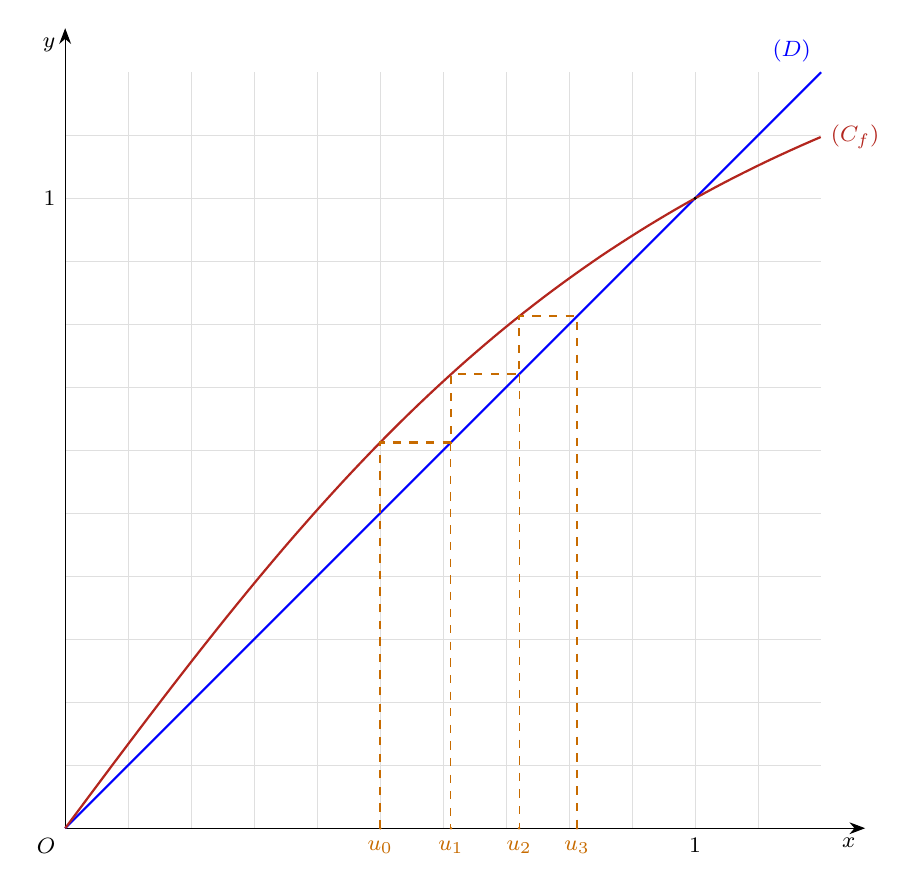
\begin{tikzpicture}[x=8cm,y=8cm,font=\footnotesize]
\draw[gray!25,very thin,step=0.1] (0,0) grid (1.2,1.2);
\draw[-{Stealth[length=2mm]}] (0,0)--(1.27,0) node[below left]{$x$};
\draw[-{Stealth[length=2mm]}] (0,0)--(0,1.27) node[below left]{$y$};
\node[below left] at (0,0){$O$};
\node[below] at (1,0){$1$}; \node[left] at (0,1){$1$};
\draw[blue,thick] (0,0)--(1.2,1.2) node[above left]{$(D)$};
\draw[cThm,thick,domain=0:1.2,samples=80] plot (\x,{3*\x/sqrt(4*\x*\x+5)});
\node[cThm,right] at (1.2,{3.6/sqrt(10.76)}){$(C_f)$};
\draw[cEx,dashed,thick] (0.5,0)--(0.5,0.6124)--(0.6124,0.6124)--(0.6124,0.7206)--(0.7206,0.7206)--(0.7206,0.8126)--(0.8126,0.8126)--(0.8126,0);
\draw[cEx,dashed] (0.6124,0.6124)--(0.6124,0) (0.7206,0.7206)--(0.7206,0);
\foreach \a/\l in {0.5/u_0,0.6124/u_1,0.7206/u_2,0.8126/u_3}{\fill[cEx] (\a,0) circle (0.5pt); \node[below,cEx] at (\a,-0.005){$\l$};}
\fill (1,1) circle (0.6pt);
\end{tikzpicture}\end{LTR}\end{center}

\pb \textbf{التخمين:} $u_0<u_1<u_2<u_3$: المتتالية $(u_n)$ متزايدة وتتقارب نحو فاصلة نقطة تقاطع $(C_f)$ و $(D)$ أي نحو $1$.

\QQ{2}
\pa \textbf{بالتراجع:} نضع $P(n)$: «$\frac12\le u_n<1$».
\begin{itemize}
\item $u_0=\frac12$ إذن $\frac12\le u_0<1$ و $P(0)$ صحيحة.
\item نفرض $\frac12\le u_n<1$. بما أنّ $f$ متزايدة تمامًا على $[0;+\infty[$: $f\left(\frac12\right)\le f(u_n)<f(1)$ أي $\frac{\sqrt6}{4}\le u_{n+1}<1$، وبما أنّ $\frac{\sqrt6}{4}\approx0{,}61>\frac12$ فإنّ $\frac12\le u_{n+1}<1$، و $P(n+1)$ صحيحة.
\item إذن من أجل كل عدد طبيعي $n$: \bx{\frac12\le u_n<1}.
\end{itemize}

\pb
\[u_{n+1}-u_n=\frac{3u_n}{\sqrt{4u_n^2+5}}-u_n=\frac{u_n\left(3-\sqrt{4u_n^2+5}\right)}{\sqrt{4u_n^2+5}}\]
بما أنّ $0<u_n<1$: $4u_n^2+5<9$ ومنه $\sqrt{4u_n^2+5}<3$ أي $3-\sqrt{4u_n^2+5}>0$، ولدينا $u_n>0$، إذن $u_{n+1}-u_n>0$ و \bxt{$(u_n)$ متزايدة تمامًا}.

$(u_n)$ متزايدة ومحدودة من الأعلى بـ $1$، إذن \bxt{$(u_n)$ متقاربة}.

\QQ{3} بما أنّ $0<u_n<1$ فإنّ $1-u_n^2\neq0$ و $v_n$ معرّف. لدينا:
\[u_{n+1}^2=\frac{9u_n^2}{4u_n^2+5}\quad;\quad1-u_{n+1}^2=\frac{4u_n^2+5-9u_n^2}{4u_n^2+5}=\frac{5\left(1-u_n^2\right)}{4u_n^2+5}\]
\[v_{n+1}=\frac{u_{n+1}^2}{1-u_{n+1}^2}=\frac{9u_n^2}{5\left(1-u_n^2\right)}=\frac95\,v_n\]
إذن $(v_n)$ هندسية أساسها $\frac95$ وحدّها الأول \bx{v_0=\dfrac{\frac14}{1-\frac14}=\frac13}.

\QQ{4}
\pa \bx{v_n=\frac13\left(\frac95\right)^n}.
من $v_n=\dfrac{u_n^2}{1-u_n^2}$: $v_n-v_nu_n^2=u_n^2$ أي $u_n^2=\dfrac{v_n}{1+v_n}$، وبما أنّ $u_n>0$:
\[u_n=\sqrt{\frac{v_n}{1+v_n}}=\sqrt{\frac{\frac13\left(\frac95\right)^n}{1+\frac13\left(\frac95\right)^n}}\qquad\text{أي}\qquad\bx{u_n=\sqrt{\frac{\left(\frac95\right)^n}{3+\left(\frac95\right)^n}}}\]

\pb $\frac95>1$ إذن $\limn\left(\frac95\right)^n=+\infty$، فنكتب $u_n=\sqrt{\dfrac{1}{3\left(\frac59\right)^n+1}}$ ومع $\limn\left(\frac59\right)^n=0$:
\[\bx{\limn u_n=\sqrt{\frac{1}{0+1}}=1}\]
(وهو ما يؤكّد التخمين.)
\end{hal}
% ================= بكالوريا 2020 م2 تقني رياضي =================
\begin{tamrin}{بكالوريا 2020 -- الموضوع الثاني -- تقني رياضي}
المتتالية العددية $(u_n)$ معرّفة بحدها الأول $u_0=\dfrac12$ ومن أجل كل عدد طبيعي $n$: $u_{n+1}=3-\dfrac{4}{u_n+2}$.

\QQ{1} برهن بالتراجع أنه من أجل كل عدد طبيعي $n$: $-1<u_n<2$.

\QQ{2}
\begin{sq}
\qa بيّن أنه من أجل كل عدد طبيعي $n$: $u_{n+1}-u_n=\dfrac{(2-u_n)(1+u_n)}{u_n+2}$.
\qb حدّد اتجاه تغير المتتالية $(u_n)$ ثم استنتج أنها متقاربة.
\end{sq}

\QQ{3} المتتالية العددية $(v_n)$ معرّفة على $\N$ بـ: $v_n=\dfrac{u_n+\alpha}{u_n+1}$، حيث $\alpha$ عدد حقيقي.
\begin{sq}
\qa أوجد $\alpha$ حتى تكون المتتالية $(v_n)$ هندسية أساسها $\dfrac14$، ثم احسب حدها الأول $v_0$.
\qb بيّن عندئذ أنه من أجل كل عدد طبيعي $n$: $u_n=\dfrac{2\times4^n-1}{4^n+1}$، ثم احسب $\limn u_n$.
\end{sq}
\end{tamrin}

\begin{hal}
\QQ{1} نضع الخاصية $P(n)$: «$-1<u_n<2$».

\textbf{التحقق:} من أجل $n=0$: $u_0=\dfrac12$ و $-1<\dfrac12<2$، إذن $P(0)$ صحيحة.

\textbf{الوراثة:} نفرض أن $P(n)$ صحيحة من أجل عدد طبيعي $n$، أي $-1<u_n<2$، ونبرهن أن $P(n+1)$ صحيحة أي $-1<u_{n+1}<2$.

لدينا $-1<u_n<2$، بإضافة $2$: $1<u_n+2<4$، وبما أن الأطراف موجبة تماما فإن بأخذ المقلوب: $\dfrac14<\dfrac{1}{u_n+2}<1$.

بالضرب في $-4$ (تنعكس المتباينات): $-4<-\dfrac{4}{u_n+2}<-1$، وبإضافة $3$: $-1<3-\dfrac{4}{u_n+2}<2$ أي $-1<u_{n+1}<2$.

إذن $P(n+1)$ صحيحة. وحسب مبدأ الاستدلال بالتراجع: \bxt{من أجل كل عدد طبيعي $n$: $-1<u_n<2$}.

\QQ{2}
\pa من أجل كل عدد طبيعي $n$ ($u_n+2\neq0$ لأن $u_n>-1$):
\[u_{n+1}-u_n=3-\frac{4}{u_n+2}-u_n=\frac{3(u_n+2)-4-u_n(u_n+2)}{u_n+2}=\frac{-u_n^2+u_n+2}{u_n+2}.\]
ومن جهة أخرى: $(2-u_n)(1+u_n)=2+2u_n-u_n-u_n^2=-u_n^2+u_n+2$. إذن:
\[\bx{u_{n+1}-u_n=\frac{(2-u_n)(1+u_n)}{u_n+2}}\]

\pb من السؤال 1: $u_n<2$ إذن $2-u_n>0$، و $u_n>-1$ إذن $1+u_n>0$ و $u_n+2>1>0$.

إذن $u_{n+1}-u_n>0$ من أجل كل $n$، ومنه \bxt{المتتالية $(u_n)$ متزايدة تماما على $\N$}.

وبما أنها متزايدة ومحدودة من الأعلى بالعدد $2$، فإن \bxt{المتتالية $(u_n)$ متقاربة}.

\QQ{3}
\pa من أجل كل $n$:
\[u_{n+1}+\alpha=\frac{3(u_n+2)-4+\alpha(u_n+2)}{u_n+2}=\frac{(3+\alpha)u_n+2+2\alpha}{u_n+2},\]
\[u_{n+1}+1=\frac{4u_n+4}{u_n+2}=\frac{4(u_n+1)}{u_n+2}.\]
إذن:
\[v_{n+1}=\frac{u_{n+1}+\alpha}{u_{n+1}+1}=\frac{(3+\alpha)u_n+2+2\alpha}{4(u_n+1)}.\]
تكون $(v_n)$ هندسية أساسها $\dfrac14$ إذا كان $v_{n+1}=\dfrac14v_n=\dfrac{u_n+\alpha}{4(u_n+1)}$ من أجل كل $n$، أي يكفي أن يكون
$(3+\alpha)u_n+2+2\alpha=u_n+\alpha$ من أجل كل $n$، ويتحقق ذلك إذا كان:
\[\begin{cases}3+\alpha=1\\ 2+2\alpha=\alpha\end{cases}\iff \alpha=-2.\]
إذن \bx{\alpha=-2} وعندئذ $v_n=\dfrac{u_n-2}{u_n+1}$ و $v_{n+1}=\dfrac{u_n-2}{4(u_n+1)}=\dfrac14v_n$.

الحد الأول: $v_0=\dfrac{\frac12-2}{\frac12+1}=\dfrac{-\frac32}{\frac32}$، أي \bx{v_0=-1}.

\pb $(v_n)$ هندسية: $v_n=v_0\times q^n=-\left(\dfrac14\right)^n=-\dfrac{1}{4^n}$.

من $v_n=\dfrac{u_n-2}{u_n+1}$: $v_n(u_n+1)=u_n-2$ أي $u_n(v_n-1)=-2-v_n$، وبما أن $v_n<0$ فإن $v_n-1\neq0$، ومنه:
\[u_n=\frac{2+v_n}{1-v_n}=\frac{2-\frac{1}{4^n}}{1+\frac{1}{4^n}}=\frac{2\times4^n-1}{4^n+1}\]
(بضرب البسط والمقام في $4^n$).
إذن \bx{u_n=\dfrac{2\times4^n-1}{4^n+1}}.

النهاية: بما أن $0<\dfrac14<1$ فإن $\limn\dfrac{1}{4^n}=0$، ومنه:
\[\limn u_n=\limn\frac{2-\frac{1}{4^n}}{1+\frac{1}{4^n}}=\frac{2-0}{1+0}\quad\Longrightarrow\quad \bx{\limn u_n=2}\]
\end{hal}

% ================= بكالوريا 2019 م1 تقني رياضي =================
\begin{tamrin}{بكالوريا 2019 -- الموضوع الأول -- تقني رياضي}
$(u_n)$ و $(v_n)$ المتتاليتان العدديتان المعرّفتان على $\N$ كما يلي:
\[\begin{cases}u_0=0\\ u_{n+1}=7u_n-18n+9\end{cases}\qquad\text{و}\qquad v_n=u_n-3n+1.\]

\QQ{1} أثبت أن المتتالية $(v_n)$ هندسية يطلب تعيين أساسها وحدها الأول.

\QQ{2} اكتب $v_n$ بدلالة $n$ ثم استنتج $u_n$ بدلالة $n$.

\QQ{3} احسب بدلالة $n$ المجموع $S_n$ حيث: $S_n=u_0+u_1+\cdots+u_n$.

\QQ{4}
\begin{sq}
\qa ادرس حسب قيم العدد الطبيعي $n$ بواقي القسمة الإقليدية لـ $7^n$ على $9$.
\qb ما هو باقي القسمة الإقليدية على $9$ للعدد $1954^{1962}+1962^{1954}+1442^{2019}$؟
\qc أثبت أنه من أجل كل عدد طبيعي $n$: $6S_n-7u_n\equiv0\,[9]$.
\end{sq}
\end{tamrin}

\begin{hal}
\QQ{1} من أجل كل عدد طبيعي $n$:
\begin{align*}
v_{n+1}&=u_{n+1}-3(n+1)+1=7u_n-18n+9-3n-3+1\\
&=7u_n-21n+7=7(u_n-3n+1)=7v_n.
\end{align*}
إذن \bxt{$(v_n)$ هندسية أساسها $q=7$} وحدها الأول $v_0=u_0-0+1$ أي \bx{v_0=1}.

\QQ{2} $v_n=v_0\times q^n$ أي \bx{v_n=7^n}. ومن $v_n=u_n-3n+1$ نجد $u_n=v_n+3n-1$ أي \bx{u_n=7^n+3n-1}.

\QQ{3}
\[S_n=\sum_{k=0}^{n}u_k=\sum_{k=0}^{n}7^k+3\sum_{k=0}^{n}k-\sum_{k=0}^{n}1.\]
\begin{itemize}
\item $\displaystyle\sum_{k=0}^{n}7^k=1\times\frac{1-7^{n+1}}{1-7}=\frac{7^{n+1}-1}{6}$ (مجموع $n+1$ حدا متتابعا لمتتالية هندسية).
\item $\displaystyle\sum_{k=0}^{n}k=0+1+\cdots+n=\frac{n(n+1)}{2}$ (مجموع حدود متتالية حسابية).
\item $\displaystyle\sum_{k=0}^{n}1=n+1$ (عدد الحدود).
\end{itemize}
إذن:
\[S_n=\frac{7^{n+1}-1}{6}+\frac{3n(n+1)}{2}-(n+1)=\frac{7^{n+1}-1}{6}+\frac{(n+1)(3n-2)}{2}.\]
\[\bx{S_n=\frac{7^{n+1}-1}{6}+\frac{(n+1)(3n-2)}{2}}\]

\QQ{4}
\pa $7^0=1$، $7^1=7$، $7^2=49=9\times5+4$ إذن $7^2\equiv4\,[9]$، $7^3=7^2\times7\equiv28\equiv1\,[9]$.

بما أن $7^3\equiv1\,[9]$ فإن البواقي دورية ودورها $3$: من أجل كل عدد طبيعي $k$:
$7^{3k}=(7^3)^k\equiv1\,[9]$، $7^{3k+1}\equiv7\,[9]$، $7^{3k+2}\equiv4\,[9]$.
\begin{center}
\begin{tabular}{|C|c|c|c|}\hline
قيم $n$ & $3k$ & $3k+1$ & $3k+2$\\\hline
باقي قسمة $7^n$ على $9$ & $1$ & $7$ & $4$\\\hline
\end{tabular}
\end{center}

\pb $1954=9\times217+1$ إذن $1954\equiv1\,[9]$ ومنه $1954^{1962}\equiv1\,[9]$.

$1962=9\times218$ إذن $1962\equiv0\,[9]$ ومنه $1962^{1954}\equiv0\,[9]$.

$1442=9\times160+2$ إذن $1442\equiv2\,[9]$. ولدينا $2\equiv-7\,[9]$ إذن $1442^{2019}\equiv(-7)^{2019}=-7^{2019}\,[9]$.

و $2019=3\times673$ إذن حسب (أ): $7^{2019}\equiv1\,[9]$، ومنه $1442^{2019}\equiv-1\equiv8\,[9]$.

إذن: $1954^{1962}+1962^{1954}+1442^{2019}\equiv1+0+8=9\equiv0\,[9]$، و \bxt{باقي القسمة على $9$ هو $0$}.

\pc لدينا $6S_n=7^{n+1}-1+3(n+1)(3n-2)=7^{n+1}-1+9n^2+3n-6$ و $7u_n=7^{n+1}+21n-7$. إذن:
\[6S_n-7u_n=9n^2+3n-7-21n+7=9n^2-18n=9(n^2-2n).\]
وبما أن $n^2-2n$ عدد صحيح فإن \bx{6S_n-7u_n\equiv0\,[9]} من أجل كل عدد طبيعي $n$.
\end{hal}

% ================= بكالوريا 2018 م1 تقني رياضي =================
\begin{tamrin}{بكالوريا 2018 -- الموضوع الأول -- تقني رياضي}
الدالة العددية المعرّفة والمتزايدة تماما على المجال $]0;+\infty[$ بـ: $f(x)=\dfrac{2x}{e\,x+1}$ ($e$ أساس اللوغاريتم النيبيري)،
و $(u_n)$ المتتالية العددية المعرّفة بحدها الأول $u_0=\dfrac{5}{4e}$ ومن أجل كل عدد طبيعي $n$: $u_{n+1}=f(u_n)$.

\QQ{1}
\begin{sq}
\qa برهن بالتراجع أنه من أجل كل عدد طبيعي $n$: $u_n>\dfrac1e$.
\qb بيّن أنه من أجل كل عدد طبيعي $n$: $u_{n+1}-u_n=\dfrac{e\,u_n\left(\frac1e-u_n\right)}{e\,u_n+1}$، ثم استنتج اتجاه تغير المتتالية $(u_n)$ وبرّر أنها متقاربة.
\end{sq}

\QQ{2} لتكن المتتالية $(v_n)$ المعرّفة من أجل كل عدد طبيعي $n$ كما يلي: $v_n=\dfrac{e\,u_n}{e\,u_n-1}$.

أثبت أن $(v_n)$ متتالية هندسية أساسها $2$، يطلب تعيين حدها الأول $v_0$ وعبارة $v_n$ بدلالة $n$.

\QQ{3}
\begin{sq}
\qa تحقق أنه من أجل كل $n$ من $\N$: $v_n=1+\dfrac{1}{e\,u_n-1}$ واستنتج عبارة $u_n$ بدلالة $n$، ثم احسب $\limn u_n$.
\qb احسب بدلالة $n$ المجموع $S_n$ حيث: $S_n=v_0+v_1+\cdots+v_n$.
\end{sq}

\QQ{4}
\begin{sq}
\qa ادرس حسب قيم العدد الطبيعي $n$ بواقي القسمة الإقليدية للعدد $2^n$ على $7$.
\qb عيّن قيم العدد الطبيعي $n$ التي من أجلها $S_n$ يقبل القسمة على $7$.
\end{sq}
\end{tamrin}

\begin{hal}
\QQ{1}
\pa نضع $P(n)$: «$u_n>\dfrac1e$».

\textbf{التحقق:} $u_0=\dfrac{5}{4e}=\dfrac54\times\dfrac1e>\dfrac1e$، إذن $P(0)$ صحيحة.

\textbf{الوراثة:} نفرض أن $u_n>\dfrac1e$ ونبرهن أن $u_{n+1}>\dfrac1e$.
بما أن $f$ متزايدة تماما على $]0;+\infty[$ و $u_n>\dfrac1e>0$ فإن $f(u_n)>f\!\left(\dfrac1e\right)$، و $f\!\left(\dfrac1e\right)=\dfrac{\frac2e}{1+1}=\dfrac1e$. إذن $u_{n+1}>\dfrac1e$، و $P(n+1)$ صحيحة.

حسب مبدأ الاستدلال بالتراجع: \bxt{من أجل كل عدد طبيعي $n$: $u_n>\dfrac1e$}.

\pb من أجل كل $n$:
\[u_{n+1}-u_n=\frac{2u_n}{e\,u_n+1}-u_n=\frac{2u_n-e\,u_n^2-u_n}{e\,u_n+1}=\frac{u_n-e\,u_n^2}{e\,u_n+1}=\frac{e\,u_n\left(\frac1e-u_n\right)}{e\,u_n+1}.\]
بما أن $u_n>\dfrac1e>0$ فإن: $e\,u_n>0$، $e\,u_n+1>0$ و $\dfrac1e-u_n<0$. إذن $u_{n+1}-u_n<0$ و \bxt{$(u_n)$ متناقصة تماما}.

وبما أنها متناقصة ومحدودة من الأسفل بالعدد $\dfrac1e$ فإن \bxt{$(u_n)$ متقاربة}.

\QQ{2} ($e\,u_n-1>0$ لأن $u_n>\frac1e$، إذن $v_n$ معرّفة.) لدينا $e\,u_{n+1}=\dfrac{2e\,u_n}{e\,u_n+1}$ و $e\,u_{n+1}-1=\dfrac{2e\,u_n-e\,u_n-1}{e\,u_n+1}=\dfrac{e\,u_n-1}{e\,u_n+1}$. إذن:
\[v_{n+1}=\frac{e\,u_{n+1}}{e\,u_{n+1}-1}=\frac{2e\,u_n}{e\,u_n+1}\times\frac{e\,u_n+1}{e\,u_n-1}=2\times\frac{e\,u_n}{e\,u_n-1}=2v_n.\]
إذن $(v_n)$ هندسية أساسها $q=2$. حدها الأول: $e\,u_0=\dfrac54$ ومنه $v_0=\dfrac{\frac54}{\frac54-1}=\dfrac{\frac54}{\frac14}$ أي \bx{v_0=5}، و \bx{v_n=5\times2^n}.

\QQ{3}
\pa $v_n=\dfrac{e\,u_n}{e\,u_n-1}=\dfrac{(e\,u_n-1)+1}{e\,u_n-1}=1+\dfrac{1}{e\,u_n-1}$ \ok.

ومنه $v_n-1=\dfrac{1}{e\,u_n-1}$ أي $e\,u_n-1=\dfrac{1}{v_n-1}$ (لأن $v_n-1=5\times2^n-1\neq0$)، إذن:
\[\bx{u_n=\frac1e\left(1+\frac{1}{5\times2^n-1}\right)}\]
بما أن $2>1$ فإن $\limn 2^n=+\infty$ ومنه $\limn\dfrac{1}{5\times2^n-1}=0$، إذن \bx{\limn u_n=\dfrac1e}.

\pb $(v_n)$ هندسية، و $S_n$ مجموع $n+1$ حدا متتابعا:
\[S_n=v_0\times\frac{1-q^{n+1}}{1-q}=5\times\frac{1-2^{n+1}}{1-2}\quad\Longrightarrow\quad\bx{S_n=5\left(2^{n+1}-1\right)}\]

\QQ{4}
\pa $2^0=1$، $2^1=2$، $2^2=4$، $2^3=8\equiv1\,[7]$. إذن البواقي دورية ودورها $3$، ومن أجل كل $k\in\N$: $2^{3k}=(2^3)^k\equiv1\,[7]$، $2^{3k+1}\equiv2\,[7]$، $2^{3k+2}\equiv4\,[7]$.
\begin{center}
\begin{tabular}{|C|c|c|c|}\hline
قيم $n$ & $3k$ & $3k+1$ & $3k+2$\\\hline
باقي قسمة $2^n$ على $7$ & $1$ & $2$ & $4$\\\hline
\end{tabular}
\end{center}

\pb $S_n\equiv0\,[7]\iff5\left(2^{n+1}-1\right)\equiv0\,[7]$. وبما أن $\pgcd(5;7)=1$ فإن (حسب مبرهنة غوص):
\[S_n\equiv0\,[7]\iff2^{n+1}\equiv1\,[7]\iff n+1=3k\ (k\in\N^*)\iff n=3k-1.\]
إذن \bxt{$S_n$ يقبل القسمة على $7$ إذا وفقط إذا كان $n=3k+2$ مع $k\in\N$}.
\end{hal}

% ================= بكالوريا 2018 م2 تقني رياضي =================
\begin{tamrin}{بكالوريا 2018 -- الموضوع الثاني -- تقني رياضي}
لتكن $(u_n)$ متتالية عددية معرّفة على $\N$ بحدها العام كما يلي: $u_n=2\times3^n$.

و $(v_n)$ متتالية عددية معرّفة بحدها الأول $v_0=4$ ومن أجل كل $n$ من $\N$: $v_{n+1}=5v_n+u_n$.

\QQ{1} نضع من أجل كل $n$ من $\N$: $w_n=\dfrac{v_n}{u_n}+\dfrac12$.

أثبت أن $(w_n)$ متتالية هندسية أساسها $\dfrac53$، يطلب تعيين حدها الأول.

\QQ{2} اكتب عبارة الحد العام $w_n$ بدلالة $n$ ثم استنتج أنه من أجل كل $n$ من $\N$: $v_n=5^{n+1}-3^n$.

\QQ{3} ادرس حسب قيم العدد الطبيعي $n$ بواقي القسمة الإقليدية للعددين $3^n$ و $5^n$ على $8$، ثم استنتج حسب قيم $n$ بواقي القسمة الإقليدية للعدد $v_n$ على $8$.
\end{tamrin}

\begin{hal}
\QQ{1} لدينا $u_{n+1}=2\times3^{n+1}=3u_n$. إذن:
\begin{align*}
w_{n+1}&=\frac{v_{n+1}}{u_{n+1}}+\frac12=\frac{5v_n+u_n}{3u_n}+\frac12=\frac53\cdot\frac{v_n}{u_n}+\frac13+\frac12\\
&=\frac53\cdot\frac{v_n}{u_n}+\frac56=\frac53\left(\frac{v_n}{u_n}+\frac12\right)=\frac53\,w_n.
\end{align*}
إذن \bxt{$(w_n)$ هندسية أساسها $q=\dfrac53$}، وحدها الأول $w_0=\dfrac{v_0}{u_0}+\dfrac12=\dfrac42+\dfrac12$ أي \bx{w_0=\dfrac52}.

\QQ{2} $w_n=w_0\times q^n$ أي \bx{w_n=\dfrac52\left(\dfrac53\right)^n}.

من تعريف $w_n$: $\dfrac{v_n}{u_n}=w_n-\dfrac12$ أي $v_n=\left(w_n-\dfrac12\right)u_n$، ومنه:
\[v_n=\left(\frac52\times\frac{5^n}{3^n}-\frac12\right)\times2\times3^n=5^{n+1}-3^n.\]
إذن \bx{v_n=5^{n+1}-3^n} من أجل كل $n$ من $\N$.

\QQ{3} \textbf{بواقي $3^n$:} $3^0=1$، $3^1=3$، $3^2=9\equiv1\,[8]$. إذن من أجل كل $k\in\N$: $3^{2k}\equiv1\,[8]$ و $3^{2k+1}\equiv3\,[8]$.

\textbf{بواقي $5^n$:} $5^0=1$، $5^1=5$، $5^2=25\equiv1\,[8]$. إذن: $5^{2k}\equiv1\,[8]$ و $5^{2k+1}\equiv5\,[8]$.

\textbf{بواقي $v_n=5\times5^n-3^n$:}
\begin{itemize}
\item إذا كان $n=2k$: $v_n\equiv5\times1-1=4\,[8]$.
\item إذا كان $n=2k+1$: $v_n\equiv5\times5-3=22\equiv6\,[8]$.
\end{itemize}
\begin{center}
\begin{tabular}{|C|c|c|}\hline
قيم $n$ & $2k$ & $2k+1$\\\hline
باقي قسمة $3^n$ على $8$ & $1$ & $3$\\\hline
باقي قسمة $5^n$ على $8$ & $1$ & $5$\\\hline
باقي قسمة $v_n$ على $8$ & $4$ & $6$\\\hline
\end{tabular}
\end{center}
\bxt{باقي قسمة $v_n$ على $8$ هو $4$ إذا كان $n$ زوجيا و $6$ إذا كان $n$ فرديا}.
\end{hal}

% ================= بكالوريا 2017 م1 تقني رياضي =================
\begin{tamrin}{بكالوريا 2017 -- الموضوع الأول -- تقني رياضي}
نعتبر الدالة العددية $f$ المعرّفة على المجال $]-\infty;1[$ بـ: $f(x)=\dfrac{1}{2-x}$. $(C)$ تمثيلها البياني في المستوي المنسوب إلى المعلم المتعامد المتجانس $(O;\vec i,\vec j)$، وليكن $(\Delta)$ المستقيم ذا المعادلة $y=x$.

$(u_n)$ المتتالية العددية المعرّفة بحدها الأول $u_0=-1$ ومن أجل كل عدد طبيعي $n$: $u_{n+1}=f(u_n)$.

\begin{GR}{-1.2}{1.2}{-0.6}{1.2}{3}
\draw[cDef,thick,domain=-1.2:0.97,samples=80] plot(\x,{1/(2-\x)});
\draw[cThm,thick] (-0.6,-0.6)--(1.2,1.2);
\node[cDef] at (-0.8,0.55){$(C)$};
\node[cThm] at (0.75,0.45){$(\Delta)$};
\end{GR}

\QQ{1} أعد رسم الشكل المقابل ثم مثّل على حامل محور الفواصل الحدود $u_0$، $u_1$، $u_2$ و $u_3$ مبرزا خطوط التمثيل، ثم ضع تخمينا حول اتجاه تغير المتتالية $(u_n)$ وتقاربها.

\QQ{2} برهن بالتراجع أنه من أجل كل عدد طبيعي $n$: $u_n<1$.

\QQ{3} ادرس اتجاه تغير المتتالية $(u_n)$ ثم استنتج أنها متقاربة.

\QQ{4} نعتبر المتتالية $(v_n)$ المعرّفة كما يلي: من أجل كل عدد طبيعي $n$: $v_n=\dfrac{2}{1-u_n}$.
\begin{sq}
\qa برهن أن المتتالية $(v_n)$ حسابية أساسها $2$ ثم عيّن عبارة حدها العام $v_n$ بدلالة $n$.
\qb استنتج عبارة الحد العام $u_n$ بدلالة $n$ واحسب $\limn u_n$.
\end{sq}
\end{tamrin}

\begin{hal}
\QQ{1} $u_0=-1$، $u_1=f(-1)=\dfrac13$، $u_2=f\!\left(\dfrac13\right)=\dfrac35$، $u_3=f\!\left(\dfrac35\right)=\dfrac57$.

ننطلق من $u_0$ على محور الفواصل، نصعد شاقوليا إلى $(C)$ فنحصل على $u_1$ ترتيبا، ثم ننقله أفقيا إلى $(\Delta)$ وننزل إلى محور الفواصل، ونكرر:
\begin{GR}{-1.2}{1.2}{-0.6}{1.2}{3}
\draw[cDef,thick,domain=-1.2:0.97,samples=80] plot(\x,{1/(2-\x)});
\draw[cThm,thick] (-0.6,-0.6)--(1.2,1.2);
\draw[cEx,thick,densely dashed] (-1,0)--(-1,1/3)--(1/3,1/3)--(1/3,3/5)--(3/5,3/5)--(3/5,5/7)--(5/7,5/7);
\draw[cEx,densely dotted] (1/3,1/3)--(1/3,0) (3/5,3/5)--(3/5,0) (5/7,5/7)--(5/7,0);
\foreach \a/\l in {-1/u_0,1/3/u_1,3/5/u_2,5/7/u_3} \fill[cEx] (\a,0) circle (1.2pt);
\node[below,font=\scriptsize] at (-1,0){$u_0$};
\node[below,font=\scriptsize] at (1/3,0){$u_1$};
\node[below,font=\scriptsize] at (0.58,0){$u_2$};
\node[below,font=\scriptsize] at (0.76,0){$u_3$};
\node[left,font=\scriptsize] at (0,1){$1$};
\node[cDef] at (-0.8,0.55){$(C)$};
\node[cThm] at (0.75,0.45){$(\Delta)$};
\end{GR}
\textbf{التخمين:} \bxt{$(u_n)$ متزايدة ومتقاربة نحو $1$} (فاصلة نقطة تقاطع $(C)$ و $(\Delta)$).

\QQ{2} نضع $P(n)$: «$u_n<1$».

\textbf{التحقق:} $u_0=-1<1$، إذن $P(0)$ صحيحة.

\textbf{الوراثة:} نفرض $u_n<1$. إذن $-u_n>-1$ ومنه $2-u_n>1>0$، وبالمقلوب: $0<\dfrac{1}{2-u_n}<1$ أي $u_{n+1}<1$. إذن $P(n+1)$ صحيحة.

حسب مبدأ الاستدلال بالتراجع: \bxt{من أجل كل عدد طبيعي $n$: $u_n<1$} (وبالتالي $u_n\in]-\infty;1[$ و $u_{n+1}=f(u_n)$ معرّف).

\QQ{3}
\[u_{n+1}-u_n=\frac{1}{2-u_n}-u_n=\frac{1-2u_n+u_n^2}{2-u_n}=\frac{(1-u_n)^2}{2-u_n}.\]
بما أن $u_n<1$ فإن $(1-u_n)^2>0$ و $2-u_n>0$، إذن $u_{n+1}-u_n>0$ و \bxt{$(u_n)$ متزايدة تماما}.

وبما أنها متزايدة ومحدودة من الأعلى بالعدد $1$، فإن \bxt{$(u_n)$ متقاربة}.

\QQ{4}
\pa ($v_n$ معرّفة لأن $1-u_n>0$.) لدينا $1-u_{n+1}=1-\dfrac{1}{2-u_n}=\dfrac{1-u_n}{2-u_n}$، إذن:
\[v_{n+1}=\frac{2}{1-u_{n+1}}=\frac{2(2-u_n)}{1-u_n}=\frac{2(1-u_n)+2}{1-u_n}=2+\frac{2}{1-u_n}=v_n+2.\]
إذن \bxt{$(v_n)$ حسابية أساسها $r=2$}، وحدها الأول $v_0=\dfrac{2}{1-(-1)}=1$، ومنه $v_n=v_0+nr$ أي \bx{v_n=2n+1}.

\pb من $v_n=\dfrac{2}{1-u_n}$: $1-u_n=\dfrac{2}{v_n}$ أي $u_n=1-\dfrac{2}{2n+1}$، إذن \bx{u_n=\dfrac{2n-1}{2n+1}}.

بما أن $\limn\dfrac{2}{2n+1}=0$ فإن \bx{\limn u_n=1}.
\end{hal}

% ================= بكالوريا 2017 م2 الدورة الاستثنائية تقني رياضي =================
\begin{tamrin}{بكالوريا 2017 -- الموضوع الثاني -- تقني رياضي -- الدورة الاستثنائية}
نعتبر المتتالية $(u_n)$ المعرّفة بـ: $u_1=\dfrac1a$ ومن أجل كل عدد طبيعي $n$ غير معدوم: $u_{n+1}=\dfrac{n+1}{a\,n}\,u_n$، حيث $a$ عدد حقيقي أكبر تماما من $2$.

\QQ{1}
\begin{sq}
\qa بيّن أنه من أجل كل عدد طبيعي $n$ غير معدوم: $u_n>0$.
\qb بيّن أن المتتالية $(u_n)$ متناقصة تماما ثم استنتج أنها متقاربة.
\end{sq}

\QQ{2} نعتبر المتتالية $(v_n)$ المعرّفة كما يلي: من أجل كل عدد طبيعي $n$ غير معدوم: $v_n=\dfrac{1}{a\,n}\,u_n$.
\begin{sq}
\qa بيّن أن المتتالية $(v_n)$ هندسية أساسها $\dfrac1a$ وعيّن حدها الأول $v_1$ بدلالة $a$.
\qb جد بدلالة $n$ و $a$ عبارة الحد العام $v_n$، ثم استنتج عبارة $u_n$ واحسب $\limn u_n$.
\end{sq}

\QQ{3} احسب بدلالة $n$ و $a$ المجموع $S_n$ حيث: $S_n=u_1+\dfrac12u_2+\dfrac13u_3+\cdots+\dfrac1n u_n$، ثم عيّن قيمة $a$ حيث $\limn S_n=\dfrac{1}{2016}$.
\end{tamrin}

\begin{molahada}[ملاحظة حول نص التمرين]
في النص المنقول: «$a$ عدد حقيقي أكبر من أو يساوي $2$». من أجل $a=2$ نجد $u_2=\dfrac{2}{2\times1}u_1=u_1=\dfrac12$، فالمتتالية لا تكون متناقصة \emph{تماما}. لذلك صحّحنا الشرط إلى $a>2$ (والقيمة المطلوبة في السؤال 3 هي $a=2017$ فلا يتأثر باقي التمرين).
\end{molahada}

\begin{hal}
\QQ{1}
\pa نضع $P(n)$: «$u_n>0$» من أجل $n\geq1$.

\textbf{التحقق:} $u_1=\dfrac1a>0$ لأن $a>2>0$، إذن $P(1)$ صحيحة.

\textbf{الوراثة:} نفرض $u_n>0$. بما أن $n+1>0$ و $a\,n>0$ فإن $\dfrac{n+1}{a\,n}>0$، ومنه $u_{n+1}=\dfrac{n+1}{a\,n}u_n>0$. إذن $P(n+1)$ صحيحة.

حسب مبدأ الاستدلال بالتراجع: \bxt{من أجل كل عدد طبيعي $n$ غير معدوم: $u_n>0$}.

\pb من أجل $n\geq1$:
\[u_{n+1}-u_n=\left(\frac{n+1}{a\,n}-1\right)u_n=\frac{n+1-a\,n}{a\,n}\,u_n=\frac{1-n(a-1)}{a\,n}\,u_n.\]
بما أن $n\geq1$ و $a-1>1$ فإن $n(a-1)>1$ أي $1-n(a-1)<0$، ومع $u_n>0$ و $a\,n>0$ نجد $u_{n+1}-u_n<0$.

إذن \bxt{$(u_n)$ متناقصة تماما}، وبما أنها محدودة من الأسفل بـ $0$ فإن \bxt{$(u_n)$ متقاربة}.

\QQ{2}
\pa من أجل $n\geq1$:
\[v_{n+1}=\frac{u_{n+1}}{a(n+1)}=\frac{1}{a(n+1)}\times\frac{n+1}{a\,n}u_n=\frac1a\times\frac{u_n}{a\,n}=\frac1a\,v_n.\]
إذن \bxt{$(v_n)$ هندسية أساسها $q=\dfrac1a$}، وحدها الأول $v_1=\dfrac{u_1}{a\times1}$ أي \bx{v_1=\dfrac{1}{a^2}}.

\pb $v_n=v_1\times q^{n-1}=\dfrac{1}{a^2}\times\dfrac{1}{a^{n-1}}$ أي \bx{v_n=\dfrac{1}{a^{n+1}}}.

ومن $v_n=\dfrac{u_n}{a\,n}$: $u_n=a\,n\,v_n=\dfrac{a\,n}{a^{n+1}}$ أي \bx{u_n=\dfrac{n}{a^n}}.

النهاية: $a^n=e^{n\ln a}$ مع $\ln a>0$، إذن $u_n=\dfrac{n}{e^{n\ln a}}=\dfrac{1}{\ln a}\times\dfrac{n\ln a}{e^{n\ln a}}$.
بوضع $X=n\ln a$: لما $n\to+\infty$ فإن $X\to+\infty$ و $\displaystyle\lim_{X\to+\infty}\frac{X}{e^X}=0$ (التزايد المقارن). إذن \bx{\limn u_n=0}.

\QQ{3} لدينا $\dfrac1k u_k=a\times\dfrac{u_k}{a\,k}=a\,v_k$، إذن:
\[S_n=a\,(v_1+v_2+\cdots+v_n)=a\times v_1\times\frac{1-q^n}{1-q}=a\times\frac{1}{a^2}\times\frac{1-\frac{1}{a^n}}{1-\frac1a}=\frac1a\times\frac{a}{a-1}\left(1-\frac{1}{a^n}\right).\]
\[\bx{S_n=\frac{1}{a-1}\left(1-\frac{1}{a^n}\right)}\]
بما أن $a>1$ فإن $\limn\dfrac{1}{a^n}=0$، ومنه $\limn S_n=\dfrac{1}{a-1}$.

$\limn S_n=\dfrac{1}{2016}\iff a-1=2016$، أي \bx{a=2017} (وهي تحقق $a>2$).
\end{hal}

% ================= بكالوريا 2016 م2 تقني رياضي =================
\begin{tamrin}{بكالوريا 2016 -- الموضوع الثاني -- تقني رياضي}
نعتبر الدالة العددية $f$ المعرّفة على المجال $[1;+\infty[$ بـ: $f(x)=\dfrac{x^2}{2x-1}$، و $(C_f)$ تمثيلها البياني في المستوي المنسوب إلى المعلم المتعامد المتجانس $(O;\vec i,\vec j)$ (الشكل المقابل).

\begin{GR}{0}{7}{0}{4}{0.9}
\draw[cDef,thick,domain=1:7,samples=80] plot(\x,{\x*\x/(2*\x-1)});
\fill[cDef] (1,1) circle (1.5pt);
\Ticks{1,2,3,4,5,6}{1,2,3}
\node[cDef] at (5.2,3.4){$(C_f)$};
\end{GR}

\QQ{1} بيّن أن الدالة $f$ متزايدة تماما على المجال $[1;+\infty[$.

\QQ{2} لتكن المتتالية العددية $(u_n)$ المعرّفة على $\N$ بـ: $u_0=6$ ومن أجل كل عدد طبيعي $n$: $u_{n+1}=f(u_n)$.
\begin{sq}
\qa انقل المنحنى المقابل ثم مثّل الحدود الأربعة الأولى للمتتالية $(u_n)$ على حامل محور الفواصل (دون حسابها) موضّحا خطوط الإنشاء.
\qb أعط تخمينا حول اتجاه تغير المتتالية $(u_n)$ وتقاربها.
\qc برهن أنه من أجل كل عدد طبيعي $n$: $1\leq u_n\leq6$.
\qd ادرس اتجاه تغير المتتالية $(u_n)$.
\qe برّر تقارب المتتالية $(u_n)$.
\end{sq}

\QQ{3} نعتبر المتتاليتين العدديتين $(v_n)$ و $(w_n)$ المعرّفتين على $\N$ بـ: $v_n=\dfrac{u_n-1}{u_n}$ و $w_n=\ln(v_n)$.
\begin{sq}
\qa برهن أن $(w_n)$ متتالية هندسية أساسها $2$، يطلب تعيين حدها الأول.
\qb اكتب $w_n$ بدلالة $n$ ثم $v_n$ بدلالة $n$.
\qc بيّن أن: $u_n=\dfrac{1}{1-\left(\frac56\right)^{2^n}}$، ثم احسب $\limn u_n$.
\end{sq}

\QQ{4} احسب بدلالة $n$ المجموع التالي: $S_n=\dfrac{1}{w_0}+\dfrac{1}{w_1}+\cdots+\dfrac{1}{w_n}$.
\end{tamrin}

\begin{hal}
\QQ{1} $f$ قابلة للاشتقاق على $[1;+\infty[$ (دالة ناطقة مقامها لا ينعدم لأن $2x-1\geq1$)، و:
\[f'(x)=\frac{2x(2x-1)-2x^2}{(2x-1)^2}=\frac{2x^2-2x}{(2x-1)^2}=\frac{2x(x-1)}{(2x-1)^2}.\]
من أجل $x>1$: $2x>0$، $x-1>0$ و $(2x-1)^2>0$ إذن $f'(x)>0$، و $f'(1)=0$ (تنعدم عند قيمة معزولة فقط).
إذن \bxt{$f$ متزايدة تماما على $[1;+\infty[$}.

\QQ{2}
\pa ننطلق من $u_0=6$، نصعد إلى $(C_f)$ ثم ننتقل أفقيا إلى المستقيم $(\Delta):y=x$ ثم ننزل إلى محور الفواصل، ونكرر:
\begin{GR}{0}{7}{0}{4}{0.9}
\draw[cDef,thick,domain=1:7,samples=80] plot(\x,{\x*\x/(2*\x-1)});
\draw[cThm,thick] (0,0)--(4,4);
\draw[cEx,thick,densely dashed] (6,0)--(6,3.2727)--(3.2727,3.2727)--(3.2727,1.9314)--(1.9314,1.9314)--(1.9314,1.3030)--(1.3030,1.3030);
\draw[cEx,densely dotted] (3.2727,3.2727)--(3.2727,0) (1.9314,1.9314)--(1.9314,0) (1.3030,1.3030)--(1.3030,0);
\foreach \a in {6,3.2727,1.9314,1.3030} \fill[cEx] (\a,0) circle (1.5pt);
\node[below,font=\scriptsize] at (6,0){$u_0$};
\node[below,font=\scriptsize] at (3.2727,0){$u_1$};
\node[below,font=\scriptsize] at (1.9314,0){$u_2$};
\node[below,font=\scriptsize] at (1.30,0){$u_3$};
\node[cDef] at (5.2,3.4){$(C_f)$};
\node[cThm] at (3.6,2.9){$(\Delta)$};
\end{GR}

\pb \textbf{التخمين:} \bxt{$(u_n)$ متناقصة ومتقاربة نحو $1$} (فاصلة نقطة تقاطع $(C_f)$ و $(\Delta)$).

\pc نضع $P(n)$: «$1\leq u_n\leq6$».

\textbf{التحقق:} $u_0=6$ و $1\leq6\leq6$، إذن $P(0)$ صحيحة.

\textbf{الوراثة:} نفرض $1\leq u_n\leq6$. بما أن $f$ متزايدة تماما على $[1;+\infty[$ فإن $f(1)\leq f(u_n)\leq f(6)$، أي $1\leq u_{n+1}\leq\dfrac{36}{11}$، و $\dfrac{36}{11}<6$. إذن $1\leq u_{n+1}\leq6$ و $P(n+1)$ صحيحة.

حسب مبدأ الاستدلال بالتراجع: \bxt{من أجل كل عدد طبيعي $n$: $1\leq u_n\leq6$}.

\pd
\[u_{n+1}-u_n=\frac{u_n^2}{2u_n-1}-u_n=\frac{u_n^2-2u_n^2+u_n}{2u_n-1}=\frac{u_n(1-u_n)}{2u_n-1}.\]
بما أن $u_n\geq1$: $u_n>0$، $2u_n-1>0$ و $1-u_n\leq0$، إذن $u_{n+1}-u_n\leq0$ و \bxt{$(u_n)$ متناقصة}.

(وبالسؤال 3 نبيّن أن $u_n>1$، فتكون متناقصة تماما.)

\pe $(u_n)$ متناقصة ومحدودة من الأسفل بالعدد $1$، إذن \bxt{$(u_n)$ متقاربة}.

\QQ{3} \textbf{تمهيد:} من أجل كل $n$: $u_n>1$. فعلا $u_0=6>1$، وإذا كان $u_n>1$ فإن $u_{n+1}-1=\dfrac{u_n^2-2u_n+1}{2u_n-1}=\dfrac{(u_n-1)^2}{2u_n-1}>0$. إذن $v_n=1-\dfrac{1}{u_n}\in\,]0;1[$ و $w_n=\ln v_n$ معرّف.

\pa لدينا $u_{n+1}-1=\dfrac{(u_n-1)^2}{2u_n-1}$ و $u_{n+1}=\dfrac{u_n^2}{2u_n-1}$، إذن:
\[v_{n+1}=\frac{u_{n+1}-1}{u_{n+1}}=\frac{(u_n-1)^2}{u_n^2}=\left(\frac{u_n-1}{u_n}\right)^2=v_n^2.\]
ومنه $w_{n+1}=\ln\left(v_n^2\right)=2\ln v_n=2w_n$. إذن \bxt{$(w_n)$ هندسية أساسها $2$}، وحدها الأول $w_0=\ln\dfrac{6-1}{6}$ أي \bx{w_0=\ln\dfrac56}.

\pb $w_n=w_0\times2^n$ أي \bx{w_n=2^n\ln\dfrac56}، ومنه $v_n=e^{w_n}=e^{2^n\ln\frac56}$ أي \bx{v_n=\left(\dfrac56\right)^{2^n}}.

\pc $v_n=1-\dfrac{1}{u_n}$ أي $\dfrac{1}{u_n}=1-v_n$ ($1-v_n\neq0$ لأن $v_n<1$)، إذن \bx{u_n=\dfrac{1}{1-\left(\frac56\right)^{2^n}}}.

بما أن $0<\dfrac56<1$ و $\limn2^n=+\infty$، فإن $\limn\left(\dfrac56\right)^{2^n}=0$ (لأن $\left(\frac56\right)^{2^n}=e^{2^n\ln\frac56}$ و $\ln\frac56<0$). إذن \bx{\limn u_n=1}.

\QQ{4} $\dfrac{1}{w_k}=\dfrac{1}{\ln\frac56}\times\left(\dfrac12\right)^k$، فحدود $\left(\dfrac{1}{w_n}\right)$ متتالية هندسية أساسها $\dfrac12$ وحدها الأول $\dfrac{1}{\ln\frac56}$:
\[S_n=\frac{1}{\ln\frac56}\times\frac{1-\left(\frac12\right)^{n+1}}{1-\frac12}=\frac{2}{\ln\frac56}\left(1-\frac{1}{2^{n+1}}\right).\]
\[\bx{S_n=\frac{2}{\ln\frac56}\left(1-\frac{1}{2^{n+1}}\right)}\]
\end{hal}

% ================= بكالوريا 2015 م1 تقني رياضي =================
\begin{tamrin}{بكالوريا 2015 -- الموضوع الأول -- تقني رياضي}
نعتبر المتتالية $(u_n)$ المعرّفة بحدها الأول $u_0=0$ ومن أجل كل عدد طبيعي $n$: $u_{n+1}=\sqrt{6u_n+16}$.

\QQ{1} $h$ الدالة المعرّفة على المجال $\left[-\dfrac83;+\infty\right[$ بما يلي: $h(x)=\sqrt{6x+16}$، و $(C)$ تمثيلها البياني في المستوي المنسوب إلى معلم متعامد ومتجانس، و $(\Delta)$ المستقيم ذو المعادلة $y=x$ (أنظر الشكل).
\begin{GR}{-3}{9}{-1}{9}{0.6}
\draw[cDef,thick,domain=-2.6667:9,samples=150] plot(\x,{sqrt(max(6*\x+16,0))});
\draw[cThm,thick] (-1,-1)--(9,9);
\Ticks{-2,2,4,6,8}{2,4,6,8}
\node[cDef] at (2.2,6.6){$(C)$};
\node[cThm] at (6.3,4.8){$(\Delta)$};
\end{GR}
\begin{sq}
\qa أعد رسم الشكل المقابل على ورقة الإجابة ثم مثّل على حامل محور الفواصل الحدود $u_0$، $u_1$، $u_2$ و $u_3$ (دون حسابها) موضّحا خطوط الإنشاء.
\qb ضع تخمينا حول اتجاه تغير $(u_n)$ وتقاربها.
\end{sq}

\QQ{2}
\begin{sq}
\qa برهن بالتراجع أنه من أجل كل عدد طبيعي $n$: $0\leq u_n<8$.
\qb بيّن أنه من أجل كل عدد طبيعي $n$: $u_{n+1}-u_n=\dfrac{(8-u_n)(u_n+2)}{\sqrt{6u_n+16}+u_n}$.
\qc استنتج اتجاه تغير $(u_n)$.
\end{sq}

\QQ{3}
\begin{sq}
\qa بيّن أنه من أجل كل عدد طبيعي $n$: $0<8-u_{n+1}\leq\dfrac12(8-u_n)$.
\qb بيّن أنه من أجل كل عدد طبيعي $n$: $0<8-u_n\leq8\left(\dfrac12\right)^n$، ثم استنتج $\limn u_n$.
\end{sq}
\end{tamrin}

\begin{hal}
\QQ{1}
\pa
\begin{GR}{-3}{9}{-1}{9}{0.6}
\draw[cDef,thick,domain=-2.6667:9,samples=150] plot(\x,{sqrt(max(6*\x+16,0))});
\draw[cThm,thick] (-1,-1)--(9,9);
\draw[cEx,thick,densely dashed] (0,0)--(0,4)--(4,4)--(4,6.3246)--(6.3246,6.3246)--(6.3246,7.3449)--(7.3449,7.3449);
\draw[cEx,densely dotted] (4,4)--(4,0) (6.3246,6.3246)--(6.3246,0) (7.3449,7.3449)--(7.3449,0);
\foreach \a in {0,4,6.3246,7.3449} \fill[cEx] (\a,0) circle (1.5pt);
\node[below right,font=\scriptsize] at (0,0){$u_0$};
\node[below,font=\scriptsize] at (4,0){$u_1$};
\node[below,font=\scriptsize] at (6.3246,0){$u_2$};
\node[below,font=\scriptsize] at (7.3449,0){$u_3$};
\node[left,font=\scriptsize] at (0,4){$4$};
\node[left,font=\scriptsize] at (0,8){$8$};
\node[below,font=\scriptsize] at (-2,0){$-2$};
\node[cDef] at (2.2,6.6){$(C)$};
\node[cThm] at (6.3,4.8){$(\Delta)$};
\end{GR}
\pb \textbf{التخمين:} \bxt{$(u_n)$ متزايدة ومتقاربة نحو $8$} (فاصلة نقطة تقاطع $(C)$ و $(\Delta)$).

\QQ{2}
\pa نضع $P(n)$: «$0\leq u_n<8$».

\textbf{التحقق:} $u_0=0$ و $0\leq0<8$، إذن $P(0)$ صحيحة.

\textbf{الوراثة:} نفرض $0\leq u_n<8$. إذن $0\leq6u_n<48$، ومنه $16\leq6u_n+16<64$. وبما أن دالة الجذر التربيعي متزايدة تماما على $[0;+\infty[$: $4\leq\sqrt{6u_n+16}<8$، أي $4\leq u_{n+1}<8$، ومنه $0\leq u_{n+1}<8$. إذن $P(n+1)$ صحيحة.

حسب مبدأ الاستدلال بالتراجع: \bxt{من أجل كل عدد طبيعي $n$: $0\leq u_n<8$}.

\pb بالضرب في المرافق ($\sqrt{6u_n+16}+u_n\geq4>0$):
\[u_{n+1}-u_n=\sqrt{6u_n+16}-u_n=\frac{(6u_n+16)-u_n^2}{\sqrt{6u_n+16}+u_n}.\]
و $-u_n^2+6u_n+16=(8-u_n)(u_n+2)$ (لأن $(8-u_n)(u_n+2)=8u_n+16-u_n^2-2u_n$). إذن:
\[\bx{u_{n+1}-u_n=\frac{(8-u_n)(u_n+2)}{\sqrt{6u_n+16}+u_n}}\]

\pc بما أن $0\leq u_n<8$: $8-u_n>0$، $u_n+2>0$ والمقام موجب تماما، إذن $u_{n+1}-u_n>0$ و \bxt{$(u_n)$ متزايدة تماما}.

\QQ{3}
\pa من السؤال 2: $u_{n+1}<8$ إذن $8-u_{n+1}>0$. ومن جهة أخرى:
\[8-u_{n+1}=8-\sqrt{6u_n+16}=\frac{64-(6u_n+16)}{8+\sqrt{6u_n+16}}=\frac{6(8-u_n)}{8+u_{n+1}}.\]
ولدينا $u_{n+1}=\sqrt{6u_n+16}\geq\sqrt{16}=4$ إذن $8+u_{n+1}\geq12$ ومنه $\dfrac{6}{8+u_{n+1}}\leq\dfrac{6}{12}=\dfrac12$. وبما أن $8-u_n>0$:
\[\bx{0<8-u_{n+1}\leq\frac12(8-u_n)}\]

\pb نبرهن بالتراجع $P(n)$: «$0<8-u_n\leq8\left(\frac12\right)^n$».

\textbf{التحقق:} $8-u_0=8$ و $8\left(\frac12\right)^0=8$، و $0<8\leq8$. إذن $P(0)$ صحيحة.

\textbf{الوراثة:} نفرض $0<8-u_n\leq8\left(\frac12\right)^n$. من (أ): $0<8-u_{n+1}\leq\dfrac12(8-u_n)\leq\dfrac12\times8\left(\dfrac12\right)^n=8\left(\dfrac12\right)^{n+1}$. إذن $P(n+1)$ صحيحة.

حسب مبدأ الاستدلال بالتراجع: \bx{0<8-u_n\leq8\left(\tfrac12\right)^n} من أجل كل $n\in\N$.

بما أن $0<\dfrac12<1$ فإن $\limn8\left(\dfrac12\right)^n=0$، وحسب مبرهنة الحصر $\limn(8-u_n)=0$، إذن \bx{\limn u_n=8}.
\end{hal}

% ================= بكالوريا 2014 م1 تقني رياضي =================
\begin{tamrin}{بكالوريا 2014 -- الموضوع الأول -- تقني رياضي}
\textbf{I)} $f$ هي الدالة المعرّفة على المجال $]1;+\infty[$ بـ: $f(x)=x-\ln(x-1)$.

\QQ{1} حدّد حسب قيم $x$ إشارة $f(x)-x$.

\QQ{2}
\begin{sq}
\qa عيّن اتجاه تغير الدالة $f$.
\qb بيّن أنه إذا كان $x\in[2;e+1]$ فإن: $f(x)\in[2;e+1]$.
\end{sq}

\textbf{II)} $(u_n)$ المتتالية المعرّفة على $\N$ بـ: $u_0=e+1$ ومن أجل كل عدد طبيعي $n$: $u_{n+1}=u_n-\ln(u_n-1)$.

\QQ{1} برهن بالتراجع أنه من أجل كل عدد طبيعي $n$: $u_n\in[2;e+1]$.

\QQ{2} ادرس اتجاه تغير المتتالية $(u_n)$.

\QQ{3} برّر تقارب المتتالية $(u_n)$، ثم احسب نهايتها.
\end{tamrin}

\begin{hal}
\textbf{I)}
\QQ{1} $f(x)-x=-\ln(x-1)$.
\begin{itemize}
\item $-\ln(x-1)=0\iff x-1=1\iff x=2$.
\item $-\ln(x-1)>0\iff\ln(x-1)<0\iff0<x-1<1\iff1<x<2$.
\item $-\ln(x-1)<0\iff x-1>1\iff x>2$.
\end{itemize}
\begin{TAB}
\tkzTabInit[lgt=2.6,espcl=3]{$x$/1,$f(x)-x$/1}{$1$,$2$,$+\infty$}
\tkzTabLine{d,+,z,-,}
\end{TAB}
إذن \bxt{$f(x)-x>0$ على $]1;2[$، $f(2)-2=0$، و $f(x)-x<0$ على $]2;+\infty[$}.

\QQ{2}
\pa $f$ قابلة للاشتقاق على $]1;+\infty[$ و: $f'(x)=1-\dfrac{1}{x-1}=\dfrac{x-2}{x-1}$.

بما أن $x-1>0$ فإن إشارة $f'(x)$ هي إشارة $x-2$.

النهايات: $\displaystyle\lim_{x\to1^+}\ln(x-1)=-\infty$ إذن $\displaystyle\lim_{x\to1^+}f(x)=+\infty$.
و $f(x)=x\left(1-\dfrac{\ln(x-1)}{x-1}\times\dfrac{x-1}{x}\right)$ مع $\displaystyle\lim_{x\to+\infty}\frac{\ln(x-1)}{x-1}=0$ و $\displaystyle\lim_{x\to+\infty}\frac{x-1}{x}=1$، إذن $\displaystyle\lim_{x\to+\infty}f(x)=+\infty$. و $f(2)=2-\ln1=2$.
\begin{TAB}
\tkzTabInit[lgt=2,espcl=3]{$x$/1,$f'(x)$/1,$f(x)$/2}{$1$,$2$,$+\infty$}
\tkzTabLine{d,-,z,+,}
\tkzTabVar{D+/$+\infty$,-/$2$,+/$+\infty$}
\end{TAB}
\bxt{$f$ متناقصة تماما على $]1;2]$ ومتزايدة تماما على $[2;+\infty[$}.

\pb إذا كان $2\leq x\leq e+1$، وبما أن $f$ متزايدة تماما على $[2;e+1]$: $f(2)\leq f(x)\leq f(e+1)$.
و $f(2)=2$، $f(e+1)=e+1-\ln e=e$. إذن $2\leq f(x)\leq e<e+1$، ومنه \bxt{$f(x)\in[2;e+1]$}.

\textbf{II)} نلاحظ أن $u_{n+1}=f(u_n)$.
\QQ{1} نضع $P(n)$: «$u_n\in[2;e+1]$».

\textbf{التحقق:} $u_0=e+1\in[2;e+1]$ (لأن $e+1\approx3{,}72>2$)، إذن $P(0)$ صحيحة.

\textbf{الوراثة:} نفرض $u_n\in[2;e+1]$؛ حسب I) 2)(ب): $f(u_n)\in[2;e+1]$ أي $u_{n+1}\in[2;e+1]$. إذن $P(n+1)$ صحيحة.

حسب مبدأ الاستدلال بالتراجع: \bxt{من أجل كل عدد طبيعي $n$: $u_n\in[2;e+1]$}.

\QQ{2} $u_{n+1}-u_n=f(u_n)-u_n=-\ln(u_n-1)$. وبما أن $u_n\geq2$ فحسب I) 1): $f(u_n)-u_n\leq0$.

إذن $u_{n+1}\leq u_n$ و \bxt{$(u_n)$ متناقصة}.

\QQ{3} $(u_n)$ متناقصة ومحدودة من الأسفل بالعدد $2$، إذن \bxt{$(u_n)$ متقاربة}. لتكن $\ell$ نهايتها؛ $\ell\in[2;e+1]$.

بما أن $f$ مستمرة على $[2;e+1]$ و $u_{n+1}=f(u_n)$، فإن $\ell=f(\ell)$ أي $-\ln(\ell-1)=0$، ومنه $\ell-1=1$. إذن \bx{\limn u_n=2}.
\end{hal}

% ================= بكالوريا 2014 م2 تقني رياضي =================

\subsection{مسائل نموذجية -- تقني رياضي}
\begin{tamrin}{بكالوريا 2014 -- الموضوع الثاني -- تقني رياضي}
$n$ و $p$ عددان طبيعيان.

\QQ{1} ادرس حسب قيم $n$ بواقي القسمة الإقليدية على $16$ للعدد $5^n$.

\QQ{2} نضع: $C_n=16n+9$ و $D_p=5^p$.
\begin{sq}
\qa بيّن أنه إذا كان $p=4k+2$ حيث $k$ عدد طبيعي، فإنه يوجد عدد طبيعي $n$ يحقق $C_n=D_p$.
\qb عيّن $n$ من أجل $p=6$.
\end{sq}

\QQ{3} $f$ هي الدالة المعرّفة على المجال $[0;+\infty[$ بـ: $f(x)=5^{4x+2}-9$.

ادرس تغيرات الدالة $f$، ثم استنتج إشارة $f(x)$.

\QQ{4} $(u_n)$ المتتالية المعرّفة على $\N$ بـ: $u_0=1$ ومن أجل كل $n$ من $\N$: $u_{n+1}=5^4\left(u_n+\dfrac{9}{16}\right)-\dfrac{9}{16}$.
\begin{sq}
\qa برهن بالتراجع أنه من أجل كل عدد طبيعي $n$: $u_n=\dfrac{5^{4n+2}-9}{16}$.
\qb برهن أنه من أجل كل عدد طبيعي $n$، فإن $u_n$ عدد طبيعي.
\end{sq}

\QQ{5} استنتج اتجاه تغير المتتالية $(u_n)$.
\end{tamrin}

\begin{hal}
\QQ{1} $5^1=5$، $5^2=25\equiv9\,[16]$، $5^3\equiv9\times5=45\equiv13\,[16]$، $5^4\equiv13\times5=65\equiv1\,[16]$.

بما أن $5^4\equiv1\,[16]$ فالبواقي دورية ودورها $4$، ومن أجل كل $k\in\N$:
\begin{center}
\begin{tabular}{|C|c|c|c|c|}\hline
قيم $n$ & $4k$ & $4k+1$ & $4k+2$ & $4k+3$\\\hline
باقي قسمة $5^n$ على $16$ & $1$ & $5$ & $9$ & $13$\\\hline
\end{tabular}
\end{center}

\QQ{2}
\pa إذا كان $p=4k+2$ فحسب الجدول: $5^p\equiv9\,[16]$، أي يوجد عدد صحيح $n$ حيث $5^p-9=16n$، أي $n=\dfrac{5^p-9}{16}$.
وبما أن $p\geq2$ فإن $5^p\geq25>9$ إذن $n>0$، فهو عدد طبيعي ويحقق $16n+9=5^p$ أي \bx{C_n=D_p}.

\pb $p=6=4\times1+2$: $16n+9=5^6=15625$ أي $16n=15616$ ومنه \bx{n=976}.

\QQ{3} $f(x)=e^{(4x+2)\ln5}-9$؛ $f$ قابلة للاشتقاق على $[0;+\infty[$ و:
\[f'(x)=4\ln5\times e^{(4x+2)\ln5}=4\ln5\times5^{4x+2}>0\quad(\ln5>0).\]
إذن $f$ متزايدة تماما على $[0;+\infty[$. $f(0)=5^2-9=16$ و $\displaystyle\lim_{x\to+\infty}f(x)=+\infty$ (لأن $(4x+2)\ln5\to+\infty$).
\begin{TAB}
\tkzTabInit[lgt=2,espcl=4]{$x$/1,$f'(x)$/1,$f(x)$/2}{$0$,$+\infty$}
\tkzTabLine{,+,}
\tkzTabVar{-/$16$,+/$+\infty$}
\end{TAB}
الإشارة: من أجل كل $x\geq0$: $f(x)\geq f(0)=16>0$، إذن \bxt{$f(x)>0$ على $[0;+\infty[$}.

\QQ{4}
\pa نضع $P(n)$: «$u_n=\dfrac{5^{4n+2}-9}{16}$».

\textbf{التحقق:} $\dfrac{5^2-9}{16}=\dfrac{16}{16}=1=u_0$، إذن $P(0)$ صحيحة.

\textbf{الوراثة:} نفرض $u_n=\dfrac{5^{4n+2}-9}{16}$. إذن $u_n+\dfrac{9}{16}=\dfrac{5^{4n+2}}{16}$ ومنه:
\[u_{n+1}=5^4\times\frac{5^{4n+2}}{16}-\frac{9}{16}=\frac{5^{4n+6}-9}{16}=\frac{5^{4(n+1)+2}-9}{16}.\]
إذن $P(n+1)$ صحيحة. حسب مبدأ الاستدلال بالتراجع: \bx{u_n=\dfrac{5^{4n+2}-9}{16}} من أجل كل $n\in\N$.

\pb $4n+2$ من الشكل $4k+2$ (مع $k=n$)، فحسب السؤال 1: $5^{4n+2}\equiv9\,[16]$ أي $16$ يقسم $5^{4n+2}-9$، إذن $u_n$ عدد صحيح. وحسب السؤال 3: $16u_n=f(n)>0$. إذن \bxt{$u_n$ عدد طبيعي} من أجل كل $n$.

\QQ{5} لدينا $u_n=\dfrac{f(n)}{16}$، وبما أن $f$ متزايدة تماما على $[0;+\infty[$ فإن $n<n+1\Rightarrow f(n)<f(n+1)$ أي $u_n<u_{n+1}$. إذن \bxt{$(u_n)$ متزايدة تماما}.

(تحقق: $u_{n+1}-u_n=\dfrac{5^{4n+6}-5^{4n+2}}{16}=\dfrac{5^{4n+2}(5^4-1)}{16}=39\times5^{4n+2}>0$.)
\end{hal}

% ================= مسألة نموذجية =================
\begin{tamrin}{مسألة نموذجية -- تقني رياضي}
نعتبر الدالة $f$ المعرّفة على المجال $[0;+\infty[$ بـ: $f(x)=6-\dfrac{5}{x+1}$، و $(C)$ تمثيلها البياني (انظر الوثيقة المرفقة).
\begin{GR}{-1}{8}{-1}{7}{0.8}
\draw[cDef,thick,domain=0:8,samples=100] plot(\x,{6-5/(\x+1)});
\draw[cThm,thick] (-1,-1)--(7,7);
\Ticks{1,2,3,4,5,6,7}{1,2,3,4,5,6}
\node[cDef] at (6.8,5.8){$(C)$};
\node[cThm] at (2.6,3.4){$(d)$};
\end{GR}

\QQ{1}
\begin{sq}
\qa ادرس تغيرات الدالة $f$ على المجال $[0;+\infty[$.
\qb حل في المجال $[0;+\infty[$ المعادلة $f(x)=x$. نرمز إلى الحل بالرمز $\alpha$.
\qc برهن أنه إذا كان $x\in[0;\alpha]$ فإن $f(x)\in[0;\alpha]$، وبالمثل إذا كان $x\in[\alpha;+\infty[$ فإن $f(x)\in[\alpha;+\infty[$.
\end{sq}

\QQ{2} نعتبر المتتالية العددية $(u_n)$ المعرّفة بحدها الأول $u_0=0$ ومن أجل كل عدد طبيعي $n$: $u_{n+1}=6-\dfrac{5}{u_n+1}$.
\begin{sq}
\qa باستعمال المنحنى $(C)$ والمستقيم $(d)$ ذي المعادلة $y=x$ مثّل الحدود $u_0$، $u_1$، $u_2$، $u_3$ و $u_4$ على محور الفواصل دون حسابها.
\qb ضع تخمينا حول اتجاه تغير المتتالية $(u_n)$ وتقاربها.
\qc برهن بالتراجع أنه من أجل كل عدد طبيعي $n$: $0\leq u_n\leq u_{n+1}\leq\alpha$.
\qd استنتج أن المتتالية $(u_n)$ متقاربة ثم عيّن نهايتها.
\end{sq}

\QQ{3} نعرّف الآن المتتالية $(u_n)$ بحد أول $u_0$ موجب أو معدوم كيفي، و $u_{n+1}=f(u_n)$. ماذا يمكن القول عن اتجاه تغير وتقارب المتتالية $(u_n)$ تبعا لقيم الحد الأول $u_0$؟
\end{tamrin}

\begin{molahada}[ملاحظة حول نص التمرين]
في النص المنقول جاء السؤال 3: «تبعا لقيم العدد الحقيقي الموجب أو المعدوم $\alpha$»، لكن $\alpha$ عدد ثابت (حل المعادلة $f(x)=x$)؛ المقصود هو الحد الأول $u_0\geq0$، فصحّحنا السؤال على هذا الأساس.
\end{molahada}

\begin{hal}
\QQ{1}
\pa $f$ قابلة للاشتقاق على $[0;+\infty[$ و $f'(x)=\dfrac{5}{(x+1)^2}>0$، إذن $f$ متزايدة تماما على $[0;+\infty[$.
$f(0)=1$ و $\displaystyle\lim_{x\to+\infty}f(x)=6$ (لأن $\frac{5}{x+1}\to0$).
\begin{TAB}
\tkzTabInit[lgt=2,espcl=4]{$x$/1,$f'(x)$/1,$f(x)$/2}{$0$,$+\infty$}
\tkzTabLine{,+,}
\tkzTabVar{-/$1$,+/$6$}
\end{TAB}

\pb من أجل $x\geq0$:
\[f(x)=x\iff6(x+1)-5=x(x+1)\iff x^2-5x-1=0.\]
المميز $\Delta=25+4=29$، والحلان $x_1=\dfrac{5+\sqrt{29}}{2}\approx5{,}19$ (مقبول) و $x_2=\dfrac{5-\sqrt{29}}{2}<0$ (مرفوض).
إذن \bx{\alpha=\dfrac{5+\sqrt{29}}{2}\approx5{,}19}.

\pc إذا كان $0\leq x\leq\alpha$، وبما أن $f$ متزايدة تماما: $f(0)\leq f(x)\leq f(\alpha)$ أي $1\leq f(x)\leq\alpha$، ومنه \bxt{$f(x)\in[0;\alpha]$}.

إذا كان $x\geq\alpha$: $f(x)\geq f(\alpha)=\alpha$، ومنه \bxt{$f(x)\in[\alpha;+\infty[$}.

\QQ{2}
\pa
\begin{GR}{-1}{8}{-1}{7}{0.8}
\draw[cDef,thick,domain=0:8,samples=100] plot(\x,{6-5/(\x+1)});
\draw[cThm,thick] (-1,-1)--(7,7);
\draw[cEx,thick,densely dashed] (0,0)--(0,1)--(1,1)--(1,3.5)--(3.5,3.5)--(3.5,4.8889)--(4.8889,4.8889)--(4.8889,5.1509)--(5.1509,5.1509);
\draw[cEx,densely dotted] (1,1)--(1,0) (3.5,3.5)--(3.5,0) (4.8889,4.8889)--(4.8889,0) (5.1509,5.1509)--(5.1509,0);
\foreach \a in {0,1,3.5,4.8889,5.1509} \fill[cEx] (\a,0) circle (1.5pt);
\node[below right,font=\scriptsize] at (0,0){$u_0$};
\node[below,font=\scriptsize] at (1,0){$u_1$};
\node[below,font=\scriptsize] at (3.5,0){$u_2$};
\node[below,font=\scriptsize] at (4.75,0){$u_3$};
\node[above right,font=\scriptsize] at (5.15,0){$u_4$};
\draw[gray,densely dotted] (5.1926,0)--(5.1926,5.1926);
\node[cDef] at (6.8,5.8){$(C)$};
\node[cThm] at (2.6,3.4){$(d)$};
\end{GR}
\pb \textbf{التخمين:} \bxt{$(u_n)$ متزايدة ومتقاربة نحو $\alpha$}.

\pc نضع $P(n)$: «$0\leq u_n\leq u_{n+1}\leq\alpha$».

\textbf{التحقق:} $u_0=0$، $u_1=6-5=1$، و $0\leq0\leq1\leq\alpha$. إذن $P(0)$ صحيحة.

\textbf{الوراثة:} نفرض $0\leq u_n\leq u_{n+1}\leq\alpha$. بما أن $f$ متزايدة تماما على $[0;+\infty[$:
$f(0)\leq f(u_n)\leq f(u_{n+1})\leq f(\alpha)$ أي $1\leq u_{n+1}\leq u_{n+2}\leq\alpha$، ومنه $0\leq u_{n+1}\leq u_{n+2}\leq\alpha$. إذن $P(n+1)$ صحيحة.

حسب مبدأ الاستدلال بالتراجع: \bxt{من أجل كل عدد طبيعي $n$: $0\leq u_n\leq u_{n+1}\leq\alpha$}.

\pd من (جـ): $(u_n)$ متزايدة ومحدودة من الأعلى بـ $\alpha$، إذن \bxt{$(u_n)$ متقاربة}. نهايتها $\ell\in[0;\alpha]$، وبما أن $f$ مستمرة على $[0;+\infty[$ فإن $f(\ell)=\ell$، والحل الوحيد في $[0;+\infty[$ هو $\alpha$. إذن \bx{\limn u_n=\alpha=\dfrac{5+\sqrt{29}}{2}}.

\QQ{3} من أجل $x\geq0$: $f(x)-x=\dfrac{-x^2+5x+1}{x+1}$، إشارته إشارة $-(x-\alpha)(x-x_2)$؛ وبما أن $x-x_2>0$:
$f(x)-x>0$ على $[0;\alpha[$، $f(\alpha)=\alpha$، و $f(x)-x<0$ على $]\alpha;+\infty[$.
\begin{itemize}
\item \textbf{إذا كان $0\leq u_0<\alpha$:} بنفس برهان 2)(جـ) ($u_0\leq u_1$ لأن $f(u_0)-u_0>0$) نجد $u_0\leq u_n\leq u_{n+1}\leq\alpha$: المتتالية \textbf{متزايدة} ومتقاربة نحو $\alpha$.
\item \textbf{إذا كان $u_0=\alpha$:} $u_1=f(\alpha)=\alpha$، وبالتراجع $u_n=\alpha$ لكل $n$: المتتالية \textbf{ثابتة} ونهايتها $\alpha$.
\item \textbf{إذا كان $u_0>\alpha$:} حسب 1)(جـ) وبالتراجع $u_n\geq\alpha$ لكل $n$ (بل $u_n>\alpha$ لأن $f$ متزايدة تماما)، ومنه $u_{n+1}-u_n=f(u_n)-u_n<0$: المتتالية \textbf{متناقصة} ومحدودة من الأسفل بـ $\alpha$، فهي متقاربة ونهايتها $\ell\geq\alpha$ تحقق $f(\ell)=\ell$، أي $\ell=\alpha$.
\end{itemize}
\bxt{مهما يكن $u_0\geq0$ فإن $(u_n)$ متقاربة ونهايتها $\alpha$}، وهي متزايدة إذا $u_0<\alpha$، ثابتة إذا $u_0=\alpha$، ومتناقصة إذا $u_0>\alpha$.
\end{hal}

% ================= مسألة نموذجية =================
\begin{tamrin}{مسألة نموذجية -- تقني رياضي}
لتكن $(u_n)$ متتالية عددية معرّفة بحدها الأول $u_0=0$ ومهما يكن $n$ من $\N$: $u_{n+1}=\dfrac{(2n+1)u_n+2}{2n+3}$.

\QQ{1}
\begin{sq}
\qa برهن بالتراجع على أنه من أجل كل عدد طبيعي $n$ فإن $u_n<1$.
\qb ادرس اتجاه تغير المتتالية $(u_n)$ واستنتج أنها متقاربة.
\end{sq}

\QQ{2} نضع من أجل كل عدد طبيعي $n$: $v_n=(2n+1)u_n$.

برهن أن المتتالية $(v_n)$ حسابية يطلب تعيين أساسها وحدها الأول.

\QQ{3} عبّر عن $v_n$ ثم $u_n$ بدلالة $n$ واحسب $\limn u_n$.

\QQ{4} نعتبر العدد $p$ حيث: $p=(1-u_0)\times(1-u_1)\times\cdots\times(1-u_n)$. بيّن أن: $p=\dfrac{2^n\,n!}{(2n+1)!}$.
\end{tamrin}

\begin{hal}
\QQ{1}
\pa نضع $P(n)$: «$u_n<1$».

\textbf{التحقق:} $u_0=0<1$، إذن $P(0)$ صحيحة.

\textbf{الوراثة:} نفرض $u_n<1$. بما أن $2n+1>0$: $(2n+1)u_n<2n+1$، ومنه $(2n+1)u_n+2<2n+3$، وبالقسمة على $2n+3>0$: $u_{n+1}<1$. إذن $P(n+1)$ صحيحة.

حسب مبدأ الاستدلال بالتراجع: \bxt{من أجل كل عدد طبيعي $n$: $u_n<1$}.

\pb
\[u_{n+1}-u_n=\frac{(2n+1)u_n+2-(2n+3)u_n}{2n+3}=\frac{2-2u_n}{2n+3}=\frac{2(1-u_n)}{2n+3}.\]
بما أن $u_n<1$ فإن $1-u_n>0$، و $2n+3>0$، إذن $u_{n+1}-u_n>0$ و \bxt{$(u_n)$ متزايدة تماما}.

وبما أنها محدودة من الأعلى بالعدد $1$ فإن \bxt{$(u_n)$ متقاربة}.

\QQ{2} $v_{n+1}=(2n+3)u_{n+1}=(2n+1)u_n+2=v_n+2$.

إذن \bxt{$(v_n)$ حسابية أساسها $r=2$} وحدها الأول $v_0=(2\times0+1)u_0$ أي \bx{v_0=0}.

\QQ{3} $v_n=v_0+nr$ أي \bx{v_n=2n}، ومنه $u_n=\dfrac{v_n}{2n+1}$ أي \bx{u_n=\dfrac{2n}{2n+1}}.

$u_n=\dfrac{2n}{2n+1}=\dfrac{2}{2+\frac1n}$ (من أجل $n\geq1$)، إذن \bx{\limn u_n=1}.

\QQ{4} من أجل كل $k\in\N$: $1-u_k=1-\dfrac{2k}{2k+1}=\dfrac{1}{2k+1}$. إذن:
\[p=\frac11\times\frac13\times\frac15\times\cdots\times\frac{1}{2n+1}=\frac{1}{1\times3\times5\times\cdots\times(2n+1)}.\]
نضرب البسط والمقام في جداء الأعداد الزوجية $2\times4\times\cdots\times(2n)=2^n\times(1\times2\times\cdots\times n)=2^n\,n!$:
\[p=\frac{2^n\,n!}{1\times2\times3\times4\times\cdots\times(2n)\times(2n+1)}\quad\Longrightarrow\quad\bx{p=\frac{2^n\,n!}{(2n+1)!}}\]
\end{hal}
% ================= مسائل نموذجية -- تقني رياضي (t3) =================
\begin{tamrin}{مسألة نموذجية -- تقني رياضي}
لتكن المتتالية العددية $(u_n)_{n\in\N}$ المعرفة كما يلي:
\[\begin{cases} u_0=\dfrac12\\[4pt] u_{n+1}=\sqrt{2u_n+3}\end{cases}\]
\QQ{1} برهن بالتراجع أنه من أجل كل عدد طبيعي $n$ فإن: $\dfrac12\le u_n<3$.

\QQ{2} أثبت أن المتتالية $(u_n)$ متزايدة تمامًا ثم استنتج أنها متقاربة محددًا نهايتها.

\QQ{3}
\begin{sq}
\qa بيّن أنه من أجل كل عدد طبيعي $n$ فإن: $|u_{n+1}-3|\le \dfrac25|u_n-3|$.
\qb استنتج أنه من أجل كل عدد طبيعي $n$ فإن: $3-u_n\le\left(\dfrac25\right)^n(3-u_0)$.
\qc استنتج من جديد نهاية المتتالية $(u_n)$.
\end{sq}
\QQ{4} نعتبر المتتالية $(v_n)_{n\in\N^*}$ المعرفة من أجل كل عدد طبيعي غير معدوم $n$ بـ: $v_n=n(3-u_n)$.
\begin{sq}
\qa بيّن أنه من أجل كل عدد طبيعي غير معدوم $n$ فإن: $\dfrac{v_{n+1}}{v_n}\le\dfrac45$.
\qb استنتج أنه من أجل كل عدد طبيعي غير معدوم $n$ فإن: $v_n\le\left(\dfrac45\right)^{n-1}$.
\qc استنتج نهاية المتتالية $(v_n)$.
\end{sq}
\end{tamrin}

\begin{hal}
\QQ{1} نسمي $P(n)$ الخاصية: «$\dfrac12\le u_n<3$».

\textbf{التحقق:} من أجل $n=0$ لدينا $u_0=\dfrac12$ و $\dfrac12\le\dfrac12<3$، إذن $P(0)$ صحيحة.

\textbf{الوراثة:} نفرض أن $P(n)$ صحيحة من أجل عدد طبيعي $n$ أي $\dfrac12\le u_n<3$، ونبرهن أن $P(n+1)$ صحيحة أي $\dfrac12\le u_{n+1}<3$.
\[\frac12\le u_n<3\ \Longrightarrow\ 1\le 2u_n<6\ \Longrightarrow\ 4\le 2u_n+3<9\ \Longrightarrow\ \sqrt4\le\sqrt{2u_n+3}<\sqrt9\]
لأن الدالة «الجذر التربيعي» متزايدة تمامًا على $[0;+\infty[$، إذن $2\le u_{n+1}<3$ ومنه $\dfrac12\le u_{n+1}<3$ (لأن $\dfrac12<2$). إذن $P(n+1)$ صحيحة.

\textbf{الخلاصة:} حسب مبدأ الاستدلال بالتراجع: \bx{\forall n\in\N:\ \dfrac12\le u_n<3}.

\QQ{2} \textbf{اتجاه التغير:} من أجل كل عدد طبيعي $n$، نضرب في المرافق:
\[u_{n+1}-u_n=\sqrt{2u_n+3}-u_n=\frac{(2u_n+3)-u_n^2}{\sqrt{2u_n+3}+u_n}=\frac{(3-u_n)(u_n+1)}{\sqrt{2u_n+3}+u_n}\]
(لأن $-u_n^2+2u_n+3=-(u_n-3)(u_n+1)=(3-u_n)(u_n+1)$).

لدينا $u_n<3$ إذن $3-u_n>0$، و$u_n\ge\dfrac12$ إذن $u_n+1>0$ والمقام $\sqrt{2u_n+3}+u_n>0$.
إذن $u_{n+1}-u_n>0$ ومنه \bxt{المتتالية $(u_n)$ متزايدة تمامًا}.

\textbf{التقارب:} $(u_n)$ متزايدة ومحدودة من الأعلى بالعدد $3$، إذن حسب مبرهنة التقارب الرتيب فهي متقاربة. لتكن $\ell$ نهايتها، مع $\dfrac12\le\ell\le3$.

الدالة $x\mapsto\sqrt{2x+3}$ مستمرة على $\left[\dfrac12;3\right]$، فبالمرور إلى النهاية في $u_{n+1}=\sqrt{2u_n+3}$ نجد:
\[\ell=\sqrt{2\ell+3}\ \Longrightarrow\ \ell^2=2\ell+3\ \Longrightarrow\ \ell^2-2\ell-3=0\ \Longrightarrow\ (\ell-3)(\ell+1)=0\]
إذن $\ell=3$ أو $\ell=-1$، والقيمة $\ell=-1$ مرفوضة لأن $\ell\ge\dfrac12$. إذن \bx{\limn u_n=3}.

\QQ{3}
\pa من أجل كل عدد طبيعي $n$:
\[u_{n+1}-3=\sqrt{2u_n+3}-3=\frac{2u_n+3-9}{\sqrt{2u_n+3}+3}=\frac{2(u_n-3)}{\sqrt{2u_n+3}+3}\]
إذن $|u_{n+1}-3|=\dfrac{2}{\sqrt{2u_n+3}+3}\,|u_n-3|$.

لدينا $u_n\ge\dfrac12$ إذن $2u_n+3\ge4$ ومنه $\sqrt{2u_n+3}\ge2$، أي $\sqrt{2u_n+3}+3\ge5$، ومنه $\dfrac{2}{\sqrt{2u_n+3}+3}\le\dfrac25$. إذن:
\[\bx{|u_{n+1}-3|\le\frac25\,|u_n-3|}\]

\pb بما أن $u_n<3$ فإن $|u_n-3|=3-u_n$، فتصبح المتباينة: $3-u_{n+1}\le\dfrac25(3-u_n)$.
نبرهن بالتراجع الخاصية $Q(n)$: «$3-u_n\le\left(\dfrac25\right)^n(3-u_0)$».
\begin{itemize}
\item من أجل $n=0$: $3-u_0\le1\times(3-u_0)$ صحيحة.
\item نفرض $3-u_n\le\left(\frac25\right)^n(3-u_0)$؛ إذن $3-u_{n+1}\le\dfrac25(3-u_n)\le\dfrac25\left(\dfrac25\right)^n(3-u_0)=\left(\dfrac25\right)^{n+1}(3-u_0)$، أي $Q(n+1)$ صحيحة.
\end{itemize}
إذن \bx{\forall n\in\N:\ 3-u_n\le\left(\frac25\right)^n(3-u_0)=\frac52\left(\frac25\right)^n}.

\pc لدينا من أجل كل $n$: $0<3-u_n\le\dfrac52\left(\dfrac25\right)^n$، و$\limn\left(\dfrac25\right)^n=0$ لأن $0<\dfrac25<1$.
حسب مبرهنة الحصر: $\limn(3-u_n)=0$ ومنه \bx{\limn u_n=3}.

\QQ{4}
\pa من أجل كل $n\ge1$ لدينا $v_n=n(3-u_n)>0$ و:
\[\frac{v_{n+1}}{v_n}=\frac{n+1}{n}\times\frac{3-u_{n+1}}{3-u_n}\]
من السؤال 3-(أ): $\dfrac{3-u_{n+1}}{3-u_n}\le\dfrac25$. ومن جهة أخرى $\dfrac{n+1}{n}=1+\dfrac1n\le2$ لأن $n\ge1$.
وبما أن جميع الكميات موجبة: $\dfrac{v_{n+1}}{v_n}\le2\times\dfrac25$، أي \bx{\frac{v_{n+1}}{v_n}\le\frac45}.

\pb لدينا $u_1=\sqrt{2\times\frac12+3}=\sqrt4=2$، إذن $v_1=1\times(3-2)=1$.
نبرهن بالتراجع أن $v_n\le\left(\frac45\right)^{n-1}$ من أجل كل $n\ge1$:
\begin{itemize}
\item من أجل $n=1$: $v_1=1\le\left(\frac45\right)^0=1$ صحيحة.
\item نفرض $v_n\le\left(\frac45\right)^{n-1}$. بما أن $v_n>0$ فإن $v_{n+1}\le\dfrac45v_n\le\dfrac45\left(\dfrac45\right)^{n-1}=\left(\dfrac45\right)^{n}$.
\end{itemize}
إذن \bx{\forall n\in\N^*:\ v_n\le\left(\frac45\right)^{n-1}}.

\pc لدينا $0<v_n\le\left(\frac45\right)^{n-1}$ و$\limn\left(\frac45\right)^{n-1}=0$ لأن $0<\frac45<1$، إذن حسب مبرهنة الحصر: \bx{\limn v_n=0}.
\end{hal}

% ------------------------------------------------------------------
\begin{tamrin}{مسألة نموذجية -- تقني رياضي}
\QQ{1} نعتبر المتتالية $(u_n)_{n\in\N}$ المعرفة بـ $u_0=\dfrac23$ ومن أجل كل عدد طبيعي $n$:
\[u_{n+1}=\frac{1}{\left(\frac{1}{u_n}-1\right)^2+1}\]
\begin{sq}
\qa احسب $u_1$ و $u_2$.
\qb برهن بالتراجع أنه من أجل كل عدد طبيعي $n$ فإن: $\dfrac12<u_n<1$.
\qc ادرس اتجاه تغير المتتالية $(u_n)$ ثم استنتج أنها متقاربة.
\end{sq}
\QQ{2} لتكن $(v_n)_{n\in\N}$ متتالية معرفة على $\N$ كما يلي: $v_n=\ln\left(\dfrac{1}{u_n}-1\right)$.
\begin{sq}
\qa بيّن أن $(v_n)$ هندسية يطلب تعيين أساسها وحدها الأول.
\qb اكتب عبارة $v_n$ بدلالة $n$ واستنتج عبارة $u_n$ بدلالة $n$.
\qc احسب بدلالة $n$ المجموع $S_n$ حيث: $S_n=\displaystyle\sum_{k=0}^{n}v_k=v_0+v_1+\dots+v_n$.
\qd احسب بدلالة $n$ الجداء $P_n$ حيث: $P_n=\displaystyle\prod_{k=0}^{n}\left(\frac{1-u_k}{u_k}\right)=\left(\frac{1-u_0}{u_0}\right)\left(\frac{1-u_1}{u_1}\right)\dots\left(\frac{1-u_n}{u_n}\right)$.
\end{sq}
\end{tamrin}

\begin{hal}
\QQ{1}
\pa $\dfrac1{u_0}-1=\dfrac32-1=\dfrac12$ إذن $u_1=\dfrac{1}{\frac14+1}=\dfrac45$.
ثم $\dfrac1{u_1}-1=\dfrac54-1=\dfrac14$ إذن $u_2=\dfrac{1}{\frac1{16}+1}=\dfrac{16}{17}$.
\[\bx{u_1=\frac45}\qquad\bx{u_2=\frac{16}{17}}\]

\pb نسمي $P(n)$ الخاصية: «$\dfrac12<u_n<1$».

\textbf{التحقق:} $u_0=\dfrac23$ و $\dfrac12<\dfrac23<1$، إذن $P(0)$ صحيحة.

\textbf{الوراثة:} نفرض $\dfrac12<u_n<1$. الدالة المقلوب متناقصة تمامًا على $]0;+\infty[$، إذن:
\[1<\frac1{u_n}<2\ \Longrightarrow\ 0<\frac1{u_n}-1<1\ \Longrightarrow\ 0<\left(\frac1{u_n}-1\right)^2<1\ \Longrightarrow\ 1<\left(\frac1{u_n}-1\right)^2+1<2\]
(لأن الدالة مربع متزايدة تمامًا على $[0;+\infty[$)، وبالمقلوب: $\dfrac12<u_{n+1}<1$. إذن $P(n+1)$ صحيحة.

\textbf{الخلاصة:} حسب مبدأ الاستدلال بالتراجع: \bx{\forall n\in\N:\ \dfrac12<u_n<1}.

\pc نضع $x_n=\dfrac1{u_n}-1$. حسب (ب): $0<x_n<1$، ولدينا $\dfrac1{u_{n+1}}=x_n^2+1$ أي $x_{n+1}=x_n^2$.
بما أن $0<x_n<1$ فإن $x_n^2<x_n$ (نضرب طرفي $x_n<1$ في $x_n>0$)، أي $x_{n+1}<x_n$، ومنه $\dfrac1{u_{n+1}}<\dfrac1{u_n}$، وبما أن الحدود موجبة: $u_{n+1}>u_n$.
إذن \bxt{المتتالية $(u_n)$ متزايدة تمامًا}.

$(u_n)$ متزايدة ومحدودة من الأعلى بالعدد $1$، إذن \bxt{$(u_n)$ متقاربة} (مبرهنة التقارب الرتيب).

\QQ{2}
\pa $v_n$ معرفة لأن $\dfrac1{u_n}-1>0$. من أجل كل عدد طبيعي $n$:
\[v_{n+1}=\ln\left(\frac1{u_{n+1}}-1\right)=\ln\left(\left(\frac1{u_n}-1\right)^2+1-1\right)=\ln\left(\frac1{u_n}-1\right)^2=2\ln\left(\frac1{u_n}-1\right)=2v_n\]
(لأن $\frac1{u_n}-1>0$). وحدها الأول $v_0=\ln\left(\frac32-1\right)=\ln\frac12=-\ln2$.

إذن \bxt{$(v_n)$ هندسية أساسها $q=2$ وحدها الأول $v_0=-\ln2$}.

\pb \bx{v_n=v_0\,q^n=-2^n\ln2}.

من $v_n=\ln\left(\dfrac1{u_n}-1\right)$ نجد $\dfrac1{u_n}-1=e^{v_n}=e^{-2^n\ln2}=2^{-2^n}$، أي $\dfrac1{u_n}=1+2^{-2^n}$، إذن:
\[\bx{u_n=\frac{1}{1+2^{-2^n}}=\frac{2^{2^n}}{2^{2^n}+1}}\]
تحقق: $u_0=\frac{2}{3}$، $u_1=\frac{4}{5}$، $u_2=\frac{16}{17}$ \ok. ونلاحظ أن $\limn 2^{-2^n}=0$ إذن $\limn u_n=1$.

\pc مجموع $n+1$ حدًّا متتابعًا من متتالية هندسية أساسها $2\ne1$:
\[S_n=v_0\times\frac{1-2^{n+1}}{1-2}=-\ln2\,(2^{n+1}-1)\qquad\text{إذن}\qquad\bx{S_n=(1-2^{n+1})\ln2}\]

\pd لدينا $\dfrac{1-u_k}{u_k}=\dfrac1{u_k}-1=e^{v_k}$، إذن:
\[P_n=e^{v_0}\times e^{v_1}\times\dots\times e^{v_n}=e^{v_0+v_1+\dots+v_n}=e^{S_n}=e^{(1-2^{n+1})\ln2}\]
إذن \bx{P_n=2^{\,1-2^{n+1}}}. (تحقق: $P_0=2^{-1}=\frac12=\frac{1-u_0}{u_0}$ \ok)
\end{hal}

% ------------------------------------------------------------------
\begin{tamrin}{مسألة نموذجية -- تقني رياضي}
نعتبر المتتالية $(u_n)$ المعرفة على $\N$ كما يلي: $u_0=1$ ومن أجل كل عدد طبيعي $n$: $u_{n+1}=\dfrac{3u_n}{u_n+1}$.

$f$ دالة عددية معرفة على $]-1;+\infty[$ كما يلي: $f(x)=\dfrac{3x}{x+1}$، و$(C_f)$ تمثيلها البياني في معلم متعامد ومتجانس $(O;\vec i,\vec j)$ (الوثيقة المرفقة).
\begin{GR}{-1}{3.5}{-1}{3}{2}
 \Ticks{1,2,3}{1,2}
 \draw[thick,cDef,domain=-0.6:3.5,samples=120,smooth] plot (\x,{3*\x/(\x+1)});
 \draw[thick,cThm] (-1,-1)--(3.5,3.5);
 \node[cDef] at (3,2.6){$(C_f)$};
 \node[cThm] at (2.9,3.3){$y=x$};
\end{GR}
\QQ{1}
\begin{sq}
\qa مثّل على الوثيقة المرفقة وعلى محور الفواصل الحدود: $u_0$، $u_1$، $u_2$ و $u_3$ مظهرًا خطوط الرسم.
\qb ضع تخمينًا حول اتجاه تغير المتتالية $(u_n)$ وتقاربها.
\end{sq}
\QQ{2}
\begin{sq}
\qa برهن بالتراجع أنه من أجل كل عدد طبيعي $n$: $0<u_n<2$.
\qb أثبت أن المتتالية $(u_n)$ متزايدة تمامًا.
\qc استنتج أنها متقاربة محددًا نهايتها.
\end{sq}
\QQ{3} نعتبر المتتالية $(v_n)$ المعرفة على $\N$ بـ: $v_n=1-\dfrac{2}{u_n}$.
\begin{sq}
\qa بيّن أن $(v_n)$ هندسية، عيّن أساسها وحدها الأول.
\qb اكتب $v_n$ بدلالة $n$ ثم استنتج $u_n$ بدلالة $n$.
\qc تحقق من نهاية $u_n$ المحسوبة في السؤال 2-(جـ).
\end{sq}
\end{tamrin}

\begin{hal}
\QQ{1}
\pa $u_1=f(u_0)=\dfrac{3}{2}=1{,}5$، $u_2=f(1{,}5)=\dfrac{4{,}5}{2{,}5}=\dfrac95=1{,}8$، $u_3=f(1{,}8)=\dfrac{5{,}4}{2{,}8}=\dfrac{27}{14}\approx1{,}93$.

\textbf{طريقة الإنشاء:} ننطلق من $u_0$ على محور الفواصل، نصعد شاقوليًّا إلى $(C_f)$ فنقرأ $u_1$ على محور التراتيب، ثم ننقله إلى محور الفواصل بواسطة المستقيم $y=x$، ونكرر.
\begin{GR}{-1}{3.5}{-1}{3}{2.4}
 \Ticks{3}{1,2}
 \draw[thick,cDef,domain=-0.6:3.5,samples=120,smooth] plot (\x,{3*\x/(\x+1)});
 \draw[thick,cThm] (-1,-1)--(3.5,3.5);
 \draw[cEx,thick] (1,0)--(1,1.5)--(1.5,1.5)--(1.5,1.8)--(1.8,1.8)--(1.8,1.92857)--(1.92857,1.92857);
 \draw[cEx,dashed] (1.5,1.5)--(1.5,0) (1.8,1.8)--(1.8,0) (1.92857,1.92857)--(1.92857,0);
 \foreach \u in {1,1.5,1.8,1.92857} \fill[cSol] (\u,0) circle (1.4pt);
 \node[below,font=\scriptsize] at (1,0){$u_0$};
 \node[below,font=\scriptsize] at (1.5,0){$u_1$};
 \node[below,font=\scriptsize] at (1.78,0){$u_2$};
 \node[above,font=\scriptsize] at (1.96,0){$u_3$};
 \node[cDef] at (3,2.55){$(C_f)$};
 \node[cThm] at (2.9,3.3){$y=x$};
\end{GR}

\pb \textbf{التخمين:} الحدود تتزايد وتقترب من فاصلة نقطة تقاطع $(C_f)$ مع المستقيم $y=x$ وهي $2$. إذن نخمّن أن \bxt{$(u_n)$ متزايدة ومتقاربة نحو $2$}.

\QQ{2}
\pa الدالة $f$ قابلة للاشتقاق على $]-1;+\infty[$ و $f'(x)=\dfrac{3(x+1)-3x}{(x+1)^2}=\dfrac{3}{(x+1)^2}>0$، إذن $f$ متزايدة تمامًا على $]-1;+\infty[$.
نسمي $P(n)$: «$0<u_n<2$».
\begin{itemize}
\item $u_0=1$ و $0<1<2$، إذن $P(0)$ صحيحة.
\item نفرض $0<u_n<2$. بما أن $f$ متزايدة تمامًا: $f(0)<f(u_n)<f(2)$، و$f(0)=0$، $f(2)=\dfrac63=2$، إذن $0<u_{n+1}<2$؛ $P(n+1)$ صحيحة.
\end{itemize}
حسب مبدأ الاستدلال بالتراجع: \bx{\forall n\in\N:\ 0<u_n<2}.

\pb من أجل كل عدد طبيعي $n$:
\[u_{n+1}-u_n=\frac{3u_n}{u_n+1}-u_n=\frac{3u_n-u_n^2-u_n}{u_n+1}=\frac{u_n(2-u_n)}{u_n+1}\]
بما أن $0<u_n<2$ فإن $u_n>0$، $2-u_n>0$ و$u_n+1>0$، إذن $u_{n+1}-u_n>0$: \bxt{$(u_n)$ متزايدة تمامًا}.

\pc $(u_n)$ متزايدة ومحدودة من الأعلى بـ$2$، إذن هي متقاربة. نهايتها $\ell$ تحقق $1\le\ell\le2$ و، لأن $f$ مستمرة على $[1;2]$، $\ell=f(\ell)$:
\[\ell=\frac{3\ell}{\ell+1}\Longrightarrow \ell^2+\ell=3\ell\Longrightarrow\ell(\ell-2)=0\]
إذن $\ell=0$ (مرفوض لأن $\ell\ge u_0=1$) أو $\ell=2$. ومنه \bx{\limn u_n=2}.

\QQ{3}
\pa $v_n$ معرفة لأن $u_n\neq0$. من أجل كل عدد طبيعي $n$:
\[v_{n+1}=1-\frac{2}{u_{n+1}}=1-\frac{2(u_n+1)}{3u_n}=\frac{3u_n-2u_n-2}{3u_n}=\frac{u_n-2}{3u_n}=\frac13\left(1-\frac2{u_n}\right)=\frac13v_n\]
و$v_0=1-\dfrac21=-1$. إذن \bxt{$(v_n)$ هندسية أساسها $q=\frac13$ وحدها الأول $v_0=-1$}.

\pb \bx{v_n=-\left(\frac13\right)^n}. ومن $v_n=1-\dfrac2{u_n}$ نجد $\dfrac2{u_n}=1-v_n$ أي $u_n=\dfrac{2}{1-v_n}$:
\[\bx{u_n=\frac{2}{1+\left(\frac13\right)^n}}\]
تحقق: $u_0=\frac22=1$، $u_1=\frac{2}{4/3}=\frac32$ \ok.

\pc بما أن $0<\frac13<1$ فإن $\limn\left(\frac13\right)^n=0$، إذن $\limn u_n=\dfrac{2}{1+0}=2$، وهي النهاية نفسها المحسوبة في السؤال 2-(جـ) \ok.
\end{hal}

% ------------------------------------------------------------------
\begin{tamrin}{مسألة نموذجية -- تقني رياضي}
\textbf{I.} نعرّف على $\N^*$ المتتالية $(u_n)$ حيث:
\[\begin{cases}u_1=e^2\\[2pt] u_{n+1}=e^{-\frac12}\sqrt{u_n}\end{cases}\]
\QQ{1} احسب كلًّا من $u_2$ و $u_3$.

\QQ{2} أثبت بالتراجع أنه من أجل كل عدد طبيعي غير معدوم $n$ فإن: $u_n>\dfrac1e$.

\QQ{3} برهن أنه من أجل كل عدد طبيعي غير معدوم $n$ فإن: $\dfrac{u_{n+1}}{u_n}<1$، ثم استنتج تقارب المتتالية $(u_n)$.

\textbf{II.} نضع من أجل كل $n$ من $\N^*$: $w_n=\dfrac12+\dfrac12\ln u_n$.

\QQ{1} أثبت أن $(w_n)$ متتالية هندسية أساسها $\dfrac12$.

\QQ{2} عبّر عن $w_n$ بدلالة $n$ ثم استنتج أن: $u_n=e^{3\left(\frac12\right)^{n-1}-1}$، ثم احسب $\limn u_n$.

\QQ{3} احسب بدلالة $n$ الجداء: $\pi_n=u_1\times u_2\times u_3\times\dots\times u_n$.
\end{tamrin}

\begin{hal}
\textbf{الجزء I}

\QQ{1} $u_2=e^{-\frac12}\sqrt{e^2}=e^{-\frac12}\times e=e^{\frac12}$، و $u_3=e^{-\frac12}\sqrt{e^{\frac12}}=e^{-\frac12}\times e^{\frac14}=e^{-\frac14}$.
\[\bx{u_2=\sqrt e}\qquad\bx{u_3=e^{-\frac14}}\]

\QQ{2} نسمي $P(n)$: «$u_n>\dfrac1e$».
\begin{itemize}
\item من أجل $n=1$: $u_1=e^2>e^{-1}=\frac1e$، إذن $P(1)$ صحيحة.
\item نفرض $u_n>\dfrac1e$. الدالة الجذر متزايدة تمامًا على $[0;+\infty[$ إذن $\sqrt{u_n}>\sqrt{e^{-1}}=e^{-\frac12}$، وبالضرب في $e^{-\frac12}>0$: $e^{-\frac12}\sqrt{u_n}>e^{-\frac12}\times e^{-\frac12}=e^{-1}$، أي $u_{n+1}>\dfrac1e$؛ $P(n+1)$ صحيحة.
\end{itemize}
حسب مبدأ الاستدلال بالتراجع: \bx{\forall n\in\N^*:\ u_n>\frac1e}.

\QQ{3} الحدود موجبة تمامًا ($u_n>\frac1e>0$)، و:
\[\frac{u_{n+1}}{u_n}=\frac{e^{-\frac12}\sqrt{u_n}}{u_n}=\frac{e^{-\frac12}}{\sqrt{u_n}}\]
بما أن $\sqrt{u_n}>e^{-\frac12}$ فإن $\dfrac{e^{-\frac12}}{\sqrt{u_n}}<1$، أي \bx{\frac{u_{n+1}}{u_n}<1}.

وبما أن $u_n>0$ فإن $u_{n+1}<u_n$: المتتالية $(u_n)$ متناقصة تمامًا، وهي محدودة من الأسفل بـ$\frac1e$، إذن \bxt{$(u_n)$ متقاربة}.

\textbf{الجزء II}

\QQ{1} من أجل كل $n\in\N^*$: $\ln u_{n+1}=\ln\left(e^{-\frac12}\sqrt{u_n}\right)=-\dfrac12+\dfrac12\ln u_n$، إذن:
\[w_{n+1}=\frac12+\frac12\ln u_{n+1}=\frac12+\frac12\left(-\frac12+\frac12\ln u_n\right)=\frac14+\frac14\ln u_n=\frac12\left(\frac12+\frac12\ln u_n\right)=\frac12w_n\]
و $w_1=\dfrac12+\dfrac12\ln e^2=\dfrac12+1=\dfrac32$. إذن \bxt{$(w_n)$ هندسية أساسها $\frac12$ وحدها الأول $w_1=\frac32$}.

\QQ{2} $w_n=w_1\,q^{\,n-1}$ إذن \bx{w_n=\frac32\left(\frac12\right)^{n-1}}.

من $w_n=\dfrac12+\dfrac12\ln u_n$: $\ln u_n=2w_n-1=3\left(\dfrac12\right)^{n-1}-1$، ومنه \bx{u_n=e^{3\left(\frac12\right)^{n-1}-1}}.

بما أن $0<\frac12<1$: $\limn\left(\frac12\right)^{n-1}=0$، إذن $\limn\left(3\left(\frac12\right)^{n-1}-1\right)=-1$، والدالة الأسية مستمرة، إذن \bx{\limn u_n=e^{-1}=\frac1e}.

\QQ{3} $\ln\pi_n=\ln u_1+\ln u_2+\dots+\ln u_n=\displaystyle\sum_{k=1}^{n}\left(3\left(\frac12\right)^{k-1}-1\right)=3\sum_{k=1}^{n}\left(\frac12\right)^{k-1}-n$.

والمجموع $\displaystyle\sum_{k=1}^{n}\left(\frac12\right)^{k-1}=\frac{1-\left(\frac12\right)^n}{1-\frac12}=2\left(1-\left(\frac12\right)^n\right)$، إذن $\ln\pi_n=6\left(1-\left(\frac12\right)^n\right)-n$:
\[\bx{\pi_n=e^{\,6-6\left(\frac12\right)^n-n}}\]
تحقق: $\pi_1=e^{6-3-1}=e^2=u_1$، $\pi_2=e^{6-\frac32-2}=e^{\frac52}=e^2\times e^{\frac12}=u_1u_2$ \ok.
\end{hal}

% ------------------------------------------------------------------
\begin{tamrin}{مسألة نموذجية -- تقني رياضي}
لتكن المتتالية العددية $(u_n)$ المعرفة بما يلي: $u_0=1$ ومن أجل كل عدد طبيعي $n$: $u_{n+1}=\dfrac{4u_n}{u_n+2}$.

\QQ{1} برهن بالتراجع أنه من أجل كل عدد طبيعي $n$: $1\le u_n<2$.

\QQ{2} ادرس رتابة المتتالية $(u_n)$. هل المتتالية $(u_n)$ متقاربة؟

\QQ{3} نضع من أجل كل عدد طبيعي $n$: $v_n=1-\dfrac{2}{u_n}$.
\begin{sq}
\qa بيّن أن المتتالية $(v_n)$ هندسية يطلب تعيين أساسها وحدها الأول، ثم عبّر عن $v_n$ بدلالة $n$.
\qb استنتج عبارة $u_n$ بدلالة $n$ ثم احسب $\limn u_n$.
\qc نضع من أجل كل عدد طبيعي $n$: $S_n=\dfrac1{u_0}+\dfrac1{u_1}+\dots+\dfrac1{u_n}$. احسب $S_n$ بدلالة $n$.
\end{sq}
\QQ{4}
\begin{sq}
\qa بيّن أن: $|u_{n+1}-2|\le\dfrac23|u_n-2|$ من أجل كل عدد طبيعي $n$.
\qb برهن أنه من أجل كل عدد طبيعي $n$: $|u_n-2|\le\left(\dfrac23\right)^n$، ثم استنتج $\limn u_n$.
\end{sq}
\end{tamrin}

\begin{molahada}
في نص المجلة كتب المجموع $S_n=\frac1{u_0}+\frac1{u_2}+\dots+\frac1{u_n}$ (سقط الحد $\frac1{u_1}$)، وهو خطأ مطبعي؛ صُحّح إلى $S_n=\frac1{u_0}+\frac1{u_1}+\dots+\frac1{u_n}$.
\end{molahada}

\begin{hal}
\QQ{1} نسمي $P(n)$: «$1\le u_n<2$».

\textbf{التحقق:} $u_0=1$ و $1\le1<2$، إذن $P(0)$ صحيحة.

\textbf{الوراثة:} نفرض $1\le u_n<2$. نكتب $u_{n+1}=\dfrac{4u_n}{u_n+2}=\dfrac{4(u_n+2)-8}{u_n+2}=4-\dfrac{8}{u_n+2}$.
\begin{align*}
1\le u_n<2&\Longrightarrow 3\le u_n+2<4\Longrightarrow\frac14<\frac1{u_n+2}\le\frac13\\
&\Longrightarrow-\frac83\le-\frac8{u_n+2}<-2\Longrightarrow\frac43\le4-\frac8{u_n+2}<2
\end{align*}
إذن $\dfrac43\le u_{n+1}<2$ وبالتالي $1\le u_{n+1}<2$؛ $P(n+1)$ صحيحة.

\textbf{الخلاصة:} \bx{\forall n\in\N:\ 1\le u_n<2}.

\QQ{2} من أجل كل عدد طبيعي $n$:
\[u_{n+1}-u_n=\frac{4u_n}{u_n+2}-u_n=\frac{4u_n-u_n^2-2u_n}{u_n+2}=\frac{u_n(2-u_n)}{u_n+2}\]
بما أن $1\le u_n<2$: $u_n>0$، $2-u_n>0$، $u_n+2>0$؛ إذن $u_{n+1}-u_n>0$ و\bxt{$(u_n)$ متزايدة تمامًا}.

$(u_n)$ متزايدة ومحدودة من الأعلى بالعدد $2$، إذن \bxt{نعم، $(u_n)$ متقاربة}.

\QQ{3}
\pa $v_n$ معرفة لأن $u_n\ge1$. من أجل كل عدد طبيعي $n$:
\[v_{n+1}=1-\frac2{u_{n+1}}=1-\frac{2(u_n+2)}{4u_n}=1-\frac{u_n+2}{2u_n}=\frac{u_n-2}{2u_n}=\frac12\left(1-\frac2{u_n}\right)=\frac12v_n\]
و $v_0=1-\dfrac21=-1$. إذن \bxt{$(v_n)$ هندسية أساسها $q=\frac12$ وحدها الأول $v_0=-1$}، و \bx{v_n=-\left(\frac12\right)^n}.

\pb من $v_n=1-\dfrac2{u_n}$: $\dfrac2{u_n}=1-v_n$، إذن $u_n=\dfrac{2}{1-v_n}$:
\[\bx{u_n=\frac{2}{1+\left(\frac12\right)^n}}\]
(تحقق: $u_0=1$، $u_1=\frac43=\frac{4\times1}{1+2}$ \ok). وبما أن $\limn\left(\frac12\right)^n=0$ (لأن $0<\frac12<1$): \bx{\limn u_n=2}.

\pc لدينا $\dfrac1{u_k}=\dfrac{1-v_k}{2}=\dfrac12+\dfrac12\left(\dfrac12\right)^k$، إذن:
\[S_n=\sum_{k=0}^{n}\frac1{u_k}=\frac{n+1}{2}+\frac12\times\frac{1-\left(\frac12\right)^{n+1}}{1-\frac12}=\frac{n+1}2+1-\left(\frac12\right)^{n+1}\]
\[\bx{S_n=\frac{n+3}{2}-\left(\frac12\right)^{n+1}}\]
تحقق: $S_0=\frac32-\frac12=1=\frac1{u_0}$ \ok.

\QQ{4}
\pa من أجل كل $n$: $u_{n+1}-2=\dfrac{4u_n-2u_n-4}{u_n+2}=\dfrac{2(u_n-2)}{u_n+2}$، إذن $|u_{n+1}-2|=\dfrac{2}{u_n+2}|u_n-2|$.
بما أن $u_n\ge1$ فإن $u_n+2\ge3$ ومنه $\dfrac2{u_n+2}\le\dfrac23$، إذن \bx{|u_{n+1}-2|\le\frac23|u_n-2|}.

\pb بالتراجع: من أجل $n=0$: $|u_0-2|=1\le\left(\frac23\right)^0=1$ صحيحة. نفرض $|u_n-2|\le\left(\frac23\right)^n$، فيكون
$|u_{n+1}-2|\le\dfrac23|u_n-2|\le\dfrac23\left(\dfrac23\right)^n=\left(\dfrac23\right)^{n+1}$. إذن \bx{\forall n\in\N:\ |u_n-2|\le\left(\frac23\right)^n}.

بما أن $0<\frac23<1$ فإن $\limn\left(\frac23\right)^n=0$، وحسب مبرهنة الحصر $\limn|u_n-2|=0$، إذن \bx{\limn u_n=2}.
\end{hal}

% ------------------------------------------------------------------
\begin{tamrin}{مسألة نموذجية -- تقني رياضي}
نعتبر الدالة $f$ المعرفة على المجال $[0;+\infty[$ كما يلي: $f(x)=\ln(x^2+4)$.

\textbf{الجزء A:}

\QQ{1} ادرس تغيرات الدالة $f$ على المجال $[0;+\infty[$.

\QQ{2} نعتبر الدالة $g$ المعرفة على $[0;+\infty[$ كما يلي: $g(x)=f(x)-x$.
\begin{sq}
\qa ادرس اتجاه تغير الدالة $g$ على المجال $[0;+\infty[$.
\qb بيّن أن المعادلة $g(x)=0$ تقبل حلًّا وحيدًا $\alpha$ من المجال $[2;3]$. احصر العدد $\alpha$ بالتقريب إلى $10^{-1}$.
\qc برّر وجود عدد حقيقي وحيد $\alpha$ (نفسه في السؤال ب) حلًّا للمعادلة $f(x)=x$.
\end{sq}
\textbf{الجزء B:} نعتبر المتتالية $(u_n)$ المعرفة بـ: $u_0=1$ ومن أجل كل عدد طبيعي $n$: $u_{n+1}=f(u_n)$.

\QQ{1} في الورقة المرفقة مثّلنا الدالة $f$ بالمنحنى $(C)$ والمستقيم $(\Delta)$ ذا المعادلة $y=x$. مثّل على محور الفواصل الحدود $u_0$، $u_1$، $u_2$، $u_3$ (دون حسابها)، موضّحًا خطوط التمثيل.

\QQ{2} علّم النقطة $I$ ذات الفاصلة $\alpha$ (نأخذ $\alpha\approx2{,}2$).

\QQ{3}
\begin{sq}
\qa برهن بالتراجع أنه من أجل كل عدد طبيعي $n$: $1\le u_n\le\alpha$.
\qb بيّن أن $(u_n)$ متقاربة، ثم عيّن نهاية المتتالية $(u_n)$.
\end{sq}
\begin{GR}{-1}{6}{-1}{4}{1.5}
 \Ticks{1,2,3,4,5}{1,2,3}
 \draw[thick,cDef,domain=0:6,samples=100,smooth] plot (\x,{ln(\x*\x+4)});
 \draw[thick,cThm,dashed] (-1,-1)--(4.5,4.5);
 \node[cDef] at (5.4,3.75){$(C)$};
 \node[cThm] at (3.3,3.7){$(\Delta)$};
\end{GR}
\end{tamrin}

\begin{hal}
\textbf{الجزء A}

\QQ{1} \textbf{النهاية:} $\displaystyle\lim_{x\to+\infty}(x^2+4)=+\infty$ و$\displaystyle\lim_{X\to+\infty}\ln X=+\infty$، إذن $\displaystyle\lim_{x\to+\infty}f(x)=+\infty$. و$f(0)=\ln4=2\ln2$.

\textbf{المشتقة:} $f$ قابلة للاشتقاق على $[0;+\infty[$ و $f'(x)=\dfrac{(x^2+4)'}{x^2+4}=\dfrac{2x}{x^2+4}$.
من أجل $x>0$: $f'(x)>0$، و$f'(0)=0$؛ إذن \bxt{$f$ متزايدة تمامًا على $[0;+\infty[$}.
\begin{TAB}
\tkzTabInit[lgt=2,espcl=4]{$x$/0.8,$f'(x)$/0.8,$f(x)$/1.6}{$0$,$+\infty$}
\tkzTabLine{z,+,}
\tkzTabVar{-/$2\ln2$,+/$+\infty$}
\end{TAB}

\QQ{2}
\pa $g$ قابلة للاشتقاق على $[0;+\infty[$ و:
\[g'(x)=f'(x)-1=\frac{2x}{x^2+4}-1=\frac{-x^2+2x-4}{x^2+4}\]
مميز $-x^2+2x-4$ هو $\Delta=4-16=-12<0$، إذن $-x^2+2x-4$ يحمل إشارة معامل $x^2$ أي سالب دائمًا، والمقام موجب. إذن $g'(x)<0$ و\bxt{$g$ متناقصة تمامًا على $[0;+\infty[$}.

النهاية عند $+\infty$: نكتب $x^2+4=x^2\left(1+\frac4{x^2}\right)$ فيكون $f(x)=2\ln x+\ln\left(1+\frac4{x^2}\right)$ من أجل $x>0$، و:
\[g(x)=x\left(\frac{2\ln x}{x}+\frac{\ln\left(1+\frac4{x^2}\right)}{x}-1\right)\]
بما أن $\displaystyle\lim_{x\to+\infty}\frac{\ln x}{x}=0$ و$\displaystyle\lim_{x\to+\infty}\ln\left(1+\frac4{x^2}\right)=0$، فإن القوس يؤول إلى $-1$، إذن $\displaystyle\lim_{x\to+\infty}g(x)=-\infty$. و$g(0)=2\ln2$.
\begin{TAB}
\tkzTabInit[lgt=2,espcl=4]{$x$/0.8,$g'(x)$/0.8,$g(x)$/1.6}{$0$,$+\infty$}
\tkzTabLine{,-,}
\tkzTabVar{+/$2\ln2$,-/$-\infty$}
\end{TAB}

\pb $g$ مستمرة ومتناقصة تمامًا على $[2;3]$، و:
\[g(2)=\ln8-2\approx0{,}079>0,\qquad g(3)=\ln13-3\approx-0{,}435<0\]
حسب مبرهنة القيم المتوسطة (حالة الرتابة التامة) المعادلة $g(x)=0$ تقبل حلًّا وحيدًا $\alpha$ في $[2;3]$.

\textbf{الحصر:} $g(2{,}1)=\ln8{,}41-2{,}1\approx0{,}029>0$ و $g(2{,}2)=\ln8{,}84-2{,}2\approx-0{,}021<0$، إذن \bx{2{,}1<\alpha<2{,}2}.

\pc $f(x)=x\iff f(x)-x=0\iff g(x)=0$. على $[0;2]$: $g(x)\ge g(2)>0$، وعلى $[3;+\infty[$: $g(x)\le g(3)<0$ (لأن $g$ متناقصة)، فلا حل خارج $[2;3]$. إذن \bxt{المعادلة $f(x)=x$ تقبل حلًّا وحيدًا هو $\alpha$ على $[0;+\infty[$}.

\textbf{الجزء B}

\QQ{1} و\textbf{2.} ننطلق من $u_0=1$ على محور الفواصل، نصعد شاقوليًّا إلى $(C)$، ثم أفقيًّا إلى $(\Delta)$، ثم نُسقط على محور الفواصل فنحصل على $u_1$، ونكرر. النقطة $I(\alpha;\alpha)$ هي نقطة تقاطع $(C)$ و$(\Delta)$.
\begin{GR}{-0.5}{3.5}{-0.5}{3}{2.6}
 \Ticks{1,3}{1,2,3}
 \draw[thick,cDef,domain=0:3.5,samples=100,smooth] plot (\x,{ln(\x*\x+4)});
 \draw[thick,cThm,dashed] (-0.5,-0.5)--(3.5,3.5);
 \draw[cEx,thick] (1,0)--(1,1.60944)--(1.60944,1.60944)--(1.60944,1.88560)--(1.88560,1.88560)--(1.88560,2.02227)--(2.02227,2.02227);
 \draw[cEx,dashed] (1.60944,1.60944)--(1.60944,0) (1.88560,1.88560)--(1.88560,0) (2.02227,2.02227)--(2.02227,0);
 \foreach \u in {1,1.60944,1.88560,2.02227} \fill[cSol] (\u,0) circle (1.3pt);
 \node[below,font=\scriptsize] at (1,0){$u_0$};
 \node[below,font=\scriptsize] at (1.61,0){$u_1$};
 \node[below,font=\scriptsize] at (1.86,0){$u_2$};
 \node[above,font=\scriptsize] at (2.04,0){$u_3$};
 \fill[cThm] (2.15873,2.15873) circle (1.6pt) node[above left]{$I$};
 \draw[cThm,dotted] (2.15873,2.15873)--(2.15873,0);
 \node[below,font=\scriptsize,cThm] at (2.25,0){$\alpha$};
 \node[cDef] at (3.1,2.75){$(C)$};
 \node[cThm] at (2.75,3.05){$(\Delta)$};
\end{GR}
نلاحظ أن الحدود تتزايد وتقترب من $\alpha$.

\QQ{3}
\pa نسمي $P(n)$: «$1\le u_n\le\alpha$».
\begin{itemize}
\item $u_0=1$ و $1\le1\le\alpha$، إذن $P(0)$ صحيحة.
\item نفرض $1\le u_n\le\alpha$. بما أن $f$ متزايدة على $[0;+\infty[$: $f(1)\le f(u_n)\le f(\alpha)$، أي $\ln5\le u_{n+1}\le\alpha$ (لأن $f(\alpha)=\alpha$). وبما أن $\ln5\approx1{,}61\ge1$ فإن $1\le u_{n+1}\le\alpha$؛ $P(n+1)$ صحيحة.
\end{itemize}
إذن \bx{\forall n\in\N:\ 1\le u_n\le\alpha}.

\pb $u_{n+1}-u_n=f(u_n)-u_n=g(u_n)$. بما أن $g$ متناقصة على $[0;+\infty[$ و$u_n\le\alpha$ فإن $g(u_n)\ge g(\alpha)=0$، إذن $u_{n+1}-u_n\ge0$: $(u_n)$ متزايدة.

$(u_n)$ متزايدة ومحدودة من الأعلى بـ$\alpha$، إذن \bxt{$(u_n)$ متقاربة}. لتكن $\ell$ نهايتها، $1\le\ell\le\alpha$. الدالة $f$ مستمرة، فبالمرور إلى النهاية $\ell=f(\ell)$ أي $g(\ell)=0$، وحسب وحدانية الحل: $\ell=\alpha$. إذن \bx{\limn u_n=\alpha}.
\end{hal}

% ------------------------------------------------------------------
\begin{tamrin}{مسألة نموذجية -- تقني رياضي}
\textbf{I.} لتكن المتتالية $(u_n)$ المعرفة على $\N$ بـ: $u_0=\dfrac13$ ومن أجل كل عدد طبيعي $n$:
\[u_{n+1}=\frac32\left[1-\frac{1}{1+2u_n}\right]\]
\QQ{1} برهن بالتراجع أنه من أجل كل عدد طبيعي $n$: $0<u_n<1$.

\QQ{2}
\begin{sq}
\qa تحقق أن: $u_{n+1}-u_n=\dfrac{2u_n(1-u_n)}{1+2u_n}$ من أجل كل عدد طبيعي $n$، ثم استنتج اتجاه تغير المتتالية $(u_n)$.
\qb بيّن أن $(u_n)$ متقاربة، ثم احسب نهايتها.
\end{sq}
\textbf{II.} لتكن $(v_n)$ متتالية عددية معرفة على $\N$ كما يلي: $v_n=-\dfrac{u_n-1}{2u_n}$.
\begin{sq}
\qa بيّن أن المتتالية $(v_n)$ هندسية يطلب تعيين أساسها وحدها الأول.
\qb اكتب $v_n$ بدلالة $n$ واستنتج $u_n$ بدلالة $n$، ثم احسب من جديد نهاية المتتالية $(u_n)$.
\qc احسب بدلالة $n$ المجموعين: $S_n=v_0+v_1+\dots+v_n$ و $T_n=\dfrac{1}{u_0}+\dfrac{3}{u_1}+\dfrac{9}{u_2}+\dots+\dfrac{3^n}{u_n}$.
\end{sq}
\end{tamrin}

\begin{molahada}
في نص المجلة: $T_n=u_0+3u_1+9u_2+\dots+3^nu_n$. هذا المجموع لا يُكتب بعبارة مغلقة بسيطة بدلالة $n$ (حده العام $\frac{9^k}{3^k+2}$)، فهو خطأ في النص. صُحّح إلى $T_n=\frac{1}{u_0}+\frac{3}{u_1}+\dots+\frac{3^n}{u_n}$ الذي حده العام $3^k+2$.
\end{molahada}

\begin{hal}
\textbf{الجزء I}

نبسّط أولًا: $1-\dfrac1{1+2u_n}=\dfrac{2u_n}{1+2u_n}$ إذن $u_{n+1}=\dfrac{3u_n}{1+2u_n}$ (ما دام $1+2u_n\neq0$).

\QQ{1} نسمي $P(n)$: «$0<u_n<1$».
\begin{itemize}
\item $u_0=\frac13$ و $0<\frac13<1$، إذن $P(0)$ صحيحة.
\item نفرض $0<u_n<1$. إذن $1+2u_n>0$ و $u_{n+1}=\dfrac{3u_n}{1+2u_n}>0$. ومن جهة أخرى:
\[1-u_{n+1}=\frac{1+2u_n-3u_n}{1+2u_n}=\frac{1-u_n}{1+2u_n}>0\]
لأن $1-u_n>0$. إذن $0<u_{n+1}<1$؛ $P(n+1)$ صحيحة.
\end{itemize}
حسب مبدأ الاستدلال بالتراجع: \bx{\forall n\in\N:\ 0<u_n<1}.

\QQ{2}
\pa $u_{n+1}-u_n=\dfrac{3u_n}{1+2u_n}-u_n=\dfrac{3u_n-u_n-2u_n^2}{1+2u_n}=\dfrac{2u_n-2u_n^2}{1+2u_n}=\dfrac{2u_n(1-u_n)}{1+2u_n}$ \ok.

بما أن $0<u_n<1$: $u_n>0$، $1-u_n>0$، $1+2u_n>0$، إذن $u_{n+1}-u_n>0$: \bxt{$(u_n)$ متزايدة تمامًا}.

\pb $(u_n)$ متزايدة ومحدودة من الأعلى بـ$1$، إذن هي متقاربة. نهايتها $\ell$ تحقق $\frac13\le\ell\le1$ و$\ell=\dfrac{3\ell}{1+2\ell}$ (الدالة $x\mapsto\frac{3x}{1+2x}$ مستمرة على $[0;1]$):
\[\ell+2\ell^2=3\ell\Longrightarrow2\ell^2-2\ell=0\Longrightarrow2\ell(\ell-1)=0\]
$\ell=0$ مرفوض لأن $\ell\ge\frac13$، إذن \bx{\limn u_n=1}.

\textbf{الجزء II}

\pa $v_n=\dfrac{1-u_n}{2u_n}$ (معرفة لأن $u_n\neq0$). من أجل كل $n$، باستعمال $1-u_{n+1}=\dfrac{1-u_n}{1+2u_n}$ و $2u_{n+1}=\dfrac{6u_n}{1+2u_n}$:
\[v_{n+1}=\frac{1-u_{n+1}}{2u_{n+1}}=\frac{1-u_n}{1+2u_n}\times\frac{1+2u_n}{6u_n}=\frac{1-u_n}{6u_n}=\frac13\times\frac{1-u_n}{2u_n}=\frac13v_n\]
و $v_0=\dfrac{1-\frac13}{2\times\frac13}=\dfrac{2/3}{2/3}=1$. إذن \bxt{$(v_n)$ هندسية أساسها $\frac13$ وحدها الأول $v_0=1$}.

\pb \bx{v_n=\left(\frac13\right)^n}. من $v_n=\dfrac{1-u_n}{2u_n}$: $2u_nv_n=1-u_n$ أي $u_n(1+2v_n)=1$، إذن:
\[\bx{u_n=\frac{1}{1+2\left(\frac13\right)^n}=\frac{3^n}{3^n+2}}\]
(تحقق: $u_0=\frac13$، $u_1=\frac35=\frac{3\times\frac13}{1+\frac23}$ \ok). وبما أن $\limn\left(\frac13\right)^n=0$: $\limn u_n=\dfrac1{1+0}=1$ \ok.

\pc $S_n$ مجموع $n+1$ حدًّا من متتالية هندسية أساسها $\frac13$:
\[S_n=1\times\frac{1-\left(\frac13\right)^{n+1}}{1-\frac13}\qquad\text{إذن}\qquad\bx{S_n=\frac32\left(1-\left(\frac13\right)^{n+1}\right)}\]
ولدينا $\dfrac1{u_k}=1+2\left(\dfrac13\right)^k$، إذن $\dfrac{3^k}{u_k}=3^k+2\times3^k\times\dfrac1{3^k}=3^k+2$، ومنه:
\[T_n=\sum_{k=0}^{n}(3^k+2)=\frac{3^{n+1}-1}{3-1}+2(n+1)\qquad\text{إذن}\qquad\bx{T_n=\frac{3^{n+1}-1}{2}+2n+2}\]
تحقق: $T_0=1+2=3=\frac1{u_0}$ \ok.
\end{hal}

% ------------------------------------------------------------------
\begin{tamrin}{مسألة نموذجية -- تقني رياضي}
نعتبر الدالة $f$ المعرفة على $\left[\dfrac12;+\infty\right[$ كما يلي: $f(x)=\dfrac{3x-1}{2x}$، وليكن $(C)$ تمثيلها البياني في المستوي المنسوب إلى معلم متعامد ومتجانس $(O;\vec i,\vec j)$.

\QQ{1} ادرس اتجاه تغير الدالة $f$ ثم أنشئ المنحنى $(C)$.

\QQ{2} $(u_n)$ متتالية عددية معرفة على $\N$ بـ $u_0=2$ ومن أجل كل عدد طبيعي $n$: $u_{n+1}=f(u_n)$.
\begin{sq}
\qa مثّل الحدود $u_0$، $u_1$، $u_2$ و $u_3$ على محور الفواصل مبرزًا خطوط الإنشاء.
\qb برهن بالتراجع أنه من أجل كل عدد طبيعي $n$: $u_n>1$.
\qc بيّن أن المتتالية $(u_n)$ متناقصة تمامًا. ماذا تستنتج؟
\end{sq}
\QQ{3}
\begin{sq}
\qa أثبت أنه من أجل كل عدد طبيعي $n$: $u_{n+1}-1\le\dfrac12(u_n-1)$.
\qb بيّن أنه من أجل كل عدد طبيعي $n$: $u_n-1\le\left(\dfrac12\right)^n$، ثم استنتج نهاية المتتالية $(u_n)$.
\end{sq}
\QQ{4} لتكن $(v_n)$ المتتالية المعرفة على $\N$ كما يلي: $v_n=\dfrac{u_n-1}{2u_n-1}$.
\begin{sq}
\qa بيّن أن $(v_n)$ هندسية يطلب تعيين أساسها وحدها الأول ثم اكتب عبارة $v_n$ بدلالة $n$.
\qb احسب المجموع $S_n$ حيث: $S_n=\dfrac{v_0-1}{u_0}+\dfrac{v_1-1}{u_1}+\dfrac{v_2-1}{u_2}+\dots+\dfrac{v_n-1}{u_n}$.
\end{sq}
\end{tamrin}

\begin{molahada}
في نص المجلة طُلب في السؤال 2-(ب) البرهان على $u_n>0$. هذا الحصر لا يكفي لإثبات التناقص في 2-(جـ) (لأن $u_{n+1}-u_n=\frac{-(2u_n-1)(u_n-1)}{2u_n}$ يتطلب $u_n>1$) ولا لحساب النهاية بالحصر في 3-(ب). صُحّح إلى $u_n>1$.
\end{molahada}

\begin{hal}
\QQ{1} \textbf{النهاية:} $\displaystyle\lim_{x\to+\infty}f(x)=\lim_{x\to+\infty}\left(\frac32-\frac1{2x}\right)=\frac32$، إذن المستقيم $y=\frac32$ مقارب أفقي لـ$(C)$ عند $+\infty$. و$f\left(\frac12\right)=\dfrac{\frac32-1}{1}=\dfrac12$.

\textbf{المشتقة:} $f(x)=\dfrac32-\dfrac1{2x}$، إذن $f'(x)=\dfrac{1}{2x^2}>0$ على $\left[\frac12;+\infty\right[$. إذن \bxt{$f$ متزايدة تمامًا على $\left[\frac12;+\infty\right[$}.
\begin{TAB}
\tkzTabInit[lgt=2,espcl=4]{$x$/0.8,$f'(x)$/0.8,$f(x)$/1.6}{$\frac12$,$+\infty$}
\tkzTabLine{,+,}
\tkzTabVar{-/$\frac12$,+/$\frac32$}
\end{TAB}
\textbf{نقط مساعدة:} $f(1)=1$، $f(2)=\frac54$، $f(4)=\frac{11}8$. حلول $f(x)=x$: $3x-1=2x^2\iff(2x-1)(x-1)=0$ أي $x=\frac12$ أو $x=1$؛ فـ$(C)$ يقطع المستقيم $y=x$ في $\left(\frac12;\frac12\right)$ و$(1;1)$.
\begin{GR}{-0.5}{5}{-0.5}{2}{2.2}
 \Ticks{1,2,3,4}{1}
 \draw[thick,cDef,domain=0.5:5,samples=100,smooth] plot (\x,{(3*\x-1)/(2*\x)});
 \draw[cThm,dashed] (-0.5,1.5)--(5,1.5);
 \draw[gray] (-0.5,-0.5)--(2,2);
 \fill[cDef] (0.5,0.5) circle (1.5pt);
 \node[cThm,above] at (4.2,1.5){$y=\frac32$};
 \node[cDef] at (3,1.1){$(C)$};
 \node[gray] at (1.75,1.95){$y=x$};
\end{GR}

\QQ{2}
\pa $u_1=f(2)=\frac54=1{,}25$، $u_2=f\left(\frac54\right)=\frac{11}{10}=1{,}1$، $u_3=f\left(\frac{11}{10}\right)=\frac{23}{22}\approx1{,}05$. ننطلق من $u_0$، نصعد إلى $(C)$ ثم ننتقل أفقيًّا إلى $y=x$ وننزل إلى محور الفواصل، ونكرر:
\begin{GR}{-0.2}{2.4}{-0.2}{1.7}{4.6}
 \Ticks{}{1}
 \draw[thick,cDef,domain=0.5:2.4,samples=100,smooth] plot (\x,{(3*\x-1)/(2*\x)});
 \draw[gray] (-0.2,-0.2)--(1.7,1.7);
 \draw[cThm,dashed] (-0.2,1.5)--(2.4,1.5);
 \draw[cEx,thick] (2,0)--(2,1.25)--(1.25,1.25)--(1.25,1.1)--(1.1,1.1)--(1.1,1.045455)--(1.045455,1.045455);
 \draw[cEx,dashed] (1.25,1.25)--(1.25,0) (1.1,1.1)--(1.1,0) (1.045455,1.045455)--(1.045455,0);
 \foreach \u in {2,1.25,1.1,1.045455} \fill[cSol] (\u,0) circle (1.3pt);
 \node[below,font=\scriptsize] at (2,0){$u_0$};
 \node[below,font=\scriptsize] at (1.25,0){$u_1$};
 \node[below,font=\scriptsize] at (1.11,0){$u_2$};
 \node[above,font=\scriptsize] at (1.03,0){$u_3$};
 \node[below,font=\scriptsize] at (0.97,0){$1$};
 \node[cDef] at (2.25,1.3){$(C)$};
 \node[gray] at (1.55,1.68){$y=x$};
\end{GR}
نلاحظ أن الحدود تتناقص وتقترب من $1$.

\pb نسمي $P(n)$: «$u_n>1$». $u_0=2>1$ إذن $P(0)$ صحيحة.
نفرض $u_n>1$؛ لدينا $u_{n+1}-1=\dfrac{3u_n-1-2u_n}{2u_n}=\dfrac{u_n-1}{2u_n}>0$ لأن $u_n-1>0$ و$2u_n>0$، إذن $u_{n+1}>1$.
(أو: $f$ متزايدة تمامًا و $u_n>1$ يعطي $f(u_n)>f(1)=1$.) إذن \bx{\forall n\in\N:\ u_n>1}.

\pc $u_{n+1}-u_n=\dfrac{3u_n-1}{2u_n}-u_n=\dfrac{-2u_n^2+3u_n-1}{2u_n}=\dfrac{-(2u_n-1)(u_n-1)}{2u_n}$.
بما أن $u_n>1$: $2u_n-1>0$، $u_n-1>0$، $2u_n>0$، إذن $u_{n+1}-u_n<0$: \bxt{$(u_n)$ متناقصة تمامًا}.

\textbf{الاستنتاج:} $(u_n)$ متناقصة ومحدودة من الأسفل بالعدد $1$، إذن \bxt{$(u_n)$ متقاربة}.

\QQ{3}
\pa من (2-ب): $u_{n+1}-1=\dfrac{u_n-1}{2u_n}$. بما أن $u_n>1$ فإن $2u_n>2$ و $\dfrac{1}{2u_n}<\dfrac12$، ومع $u_n-1>0$:
\[\bx{u_{n+1}-1\le\frac12(u_n-1)}\]

\pb بالتراجع: $n=0$: $u_0-1=1\le\left(\frac12\right)^0=1$ صحيحة. نفرض $u_n-1\le\left(\frac12\right)^n$؛ إذن $u_{n+1}-1\le\frac12(u_n-1)\le\frac12\left(\frac12\right)^n=\left(\frac12\right)^{n+1}$. إذن \bx{\forall n\in\N:\ u_n-1\le\left(\frac12\right)^n}.

لدينا $0<u_n-1\le\left(\frac12\right)^n$ و$\limn\left(\frac12\right)^n=0$، فحسب مبرهنة الحصر $\limn(u_n-1)=0$، إذن \bx{\limn u_n=1}.

\QQ{4}
\pa $v_n$ معرفة لأن $2u_n-1>1>0$. نحسب: $u_{n+1}-1=\dfrac{u_n-1}{2u_n}$ و $2u_{n+1}-1=\dfrac{3u_n-1}{u_n}-1=\dfrac{2u_n-1}{u_n}$، إذن:
\[v_{n+1}=\frac{u_n-1}{2u_n}\times\frac{u_n}{2u_n-1}=\frac12\times\frac{u_n-1}{2u_n-1}=\frac12v_n\]
و $v_0=\dfrac{2-1}{4-1}=\dfrac13$. إذن \bxt{$(v_n)$ هندسية أساسها $\frac12$ وحدها الأول $v_0=\frac13$}، و \bx{v_n=\frac13\left(\frac12\right)^n}.

\pb نحسب $\dfrac{v_k-1}{u_k}$: لدينا $v_k-1=\dfrac{u_k-1-2u_k+1}{2u_k-1}=\dfrac{-u_k}{2u_k-1}$، إذن $\dfrac{v_k-1}{u_k}=\dfrac{-1}{2u_k-1}$.
ومن جهة أخرى $1-2v_k=\dfrac{2u_k-1-2u_k+2}{2u_k-1}=\dfrac{1}{2u_k-1}$، إذن $\dfrac{v_k-1}{u_k}=2v_k-1$. ومنه:
\[S_n=\sum_{k=0}^{n}(2v_k-1)=2\sum_{k=0}^{n}v_k-(n+1)=2\times\frac13\times\frac{1-\left(\frac12\right)^{n+1}}{1-\frac12}-(n+1)\]
\[\bx{S_n=\frac43\left(1-\left(\frac12\right)^{n+1}\right)-n-1}\]
تحقق: $S_0=\frac43\times\frac12-1=-\frac13$، و $\frac{v_0-1}{u_0}=\frac{-2/3}{2}=-\frac13$ \ok.
\end{hal}

% ------------------------------------------------------------------
\begin{tamrin}{مسألة نموذجية -- تقني رياضي}
نعتبر المتتالية $(u_n)$ المعرفة على $\N$ كما يلي: $u_0=-1$ و $u_1=\dfrac12$ ومن أجل كل عدد طبيعي $n$:
\[u_{n+2}=u_{n+1}-\frac14u_n\]
\QQ{1} احسب $u_2$ ثم استنتج أن المتتالية $(u_n)$ لا حسابية ولا هندسية.

\QQ{2} نعرّف المتتالية $(v_n)$ من أجل كل عدد طبيعي $n$ كما يلي: $v_n=u_{n+1}-\dfrac12u_n$.
\begin{sq}
\qa احسب $v_0$ ثم عبّر عن $v_{n+1}$ بدلالة $v_n$.
\qb استنتج أن المتتالية $(v_n)$ هندسية يطلب تعيين أساسها، ثم اكتب عبارة $v_n$ بدلالة $n$.
\end{sq}
\QQ{3} نعرّف المتتالية $(w_n)$ كما يلي: من أجل كل عدد طبيعي $n$: $w_n=\dfrac{u_n}{v_n}$.
\begin{sq}
\qa احسب $w_0$ ثم باستعمال المساواة $u_{n+1}=v_n+\dfrac12u_n$، عبّر عن $w_{n+1}$ بدلالة $v_n$ و $u_n$.
\qb استنتج أنه من أجل كل عدد طبيعي $n$ فإن: $w_{n+1}=w_n+2$، ثم عبّر عن $w_n$ بدلالة $n$.
\end{sq}
\QQ{4} بيّن أنه من أجل كل عدد طبيعي $n$ فإن: $u_n=\dfrac{2n-1}{2^n}$.

\QQ{5} نضع من أجل كل عدد طبيعي $n$: $S_n=u_0+u_1+\dots+u_n$. برهن بالتراجع أنه من أجل كل عدد طبيعي $n$ فإن: $S_n=2-\dfrac{2n+3}{2^n}$.
\end{tamrin}

\begin{hal}
\QQ{1} $u_2=u_1-\dfrac14u_0=\dfrac12+\dfrac14$، إذن \bx{u_2=\frac34}.

$u_1-u_0=\dfrac32$ و $u_2-u_1=\dfrac14$؛ بما أن $u_2-u_1\neq u_1-u_0$ فإن $(u_n)$ ليست حسابية.

$\dfrac{u_1}{u_0}=-\dfrac12$ و $\dfrac{u_2}{u_1}=\dfrac32$؛ بما أن $\dfrac{u_2}{u_1}\neq\dfrac{u_1}{u_0}$ فإن $(u_n)$ ليست هندسية.

إذن \bxt{$(u_n)$ لا حسابية ولا هندسية}.

\QQ{2}
\pa $v_0=u_1-\dfrac12u_0=\dfrac12+\dfrac12$، أي \bx{v_0=1}. ومن أجل كل $n$:
\[v_{n+1}=u_{n+2}-\frac12u_{n+1}=u_{n+1}-\frac14u_n-\frac12u_{n+1}=\frac12u_{n+1}-\frac14u_n=\frac12\left(u_{n+1}-\frac12u_n\right)\]
إذن \bx{v_{n+1}=\frac12v_n}.

\pb إذن \bxt{$(v_n)$ هندسية أساسها $\frac12$ وحدها الأول $v_0=1$}، و \bx{v_n=\left(\frac12\right)^n=\frac1{2^n}}.

\QQ{3}
\pa $v_n\neq0$ إذن $w_n$ معرفة، و $w_0=\dfrac{u_0}{v_0}=\dfrac{-1}{1}$ أي \bx{w_0=-1}.
من تعريف $v_n$: $u_{n+1}=v_n+\frac12u_n$، ومع $v_{n+1}=\frac12v_n$:
\[\bx{w_{n+1}=\frac{u_{n+1}}{v_{n+1}}=\frac{v_n+\frac12u_n}{\frac12v_n}}\]

\pb $w_{n+1}=\dfrac{v_n}{\frac12v_n}+\dfrac{\frac12u_n}{\frac12v_n}=2+\dfrac{u_n}{v_n}$، أي \bx{w_{n+1}=w_n+2}.
إذن $(w_n)$ حسابية أساسها $2$ وحدها الأول $w_0=-1$، ومنه \bx{w_n=-1+2n=2n-1}.

\QQ{4} $u_n=w_n\times v_n=(2n-1)\times\dfrac1{2^n}$، إذن \bx{u_n=\frac{2n-1}{2^n}}.
(تحقق: $u_0=-1$، $u_1=\frac12$، $u_2=\frac34$ \ok)

\QQ{5} نسمي $P(n)$: «$S_n=2-\dfrac{2n+3}{2^n}$».

\textbf{التحقق:} $S_0=u_0=-1$ و $2-\dfrac{3}{1}=-1$، إذن $P(0)$ صحيحة.

\textbf{الوراثة:} نفرض $S_n=2-\dfrac{2n+3}{2^n}$ ونبرهن $S_{n+1}=2-\dfrac{2n+5}{2^{n+1}}$:
\[S_{n+1}=S_n+u_{n+1}=2-\frac{2n+3}{2^n}+\frac{2n+1}{2^{n+1}}=2-\frac{2(2n+3)-(2n+1)}{2^{n+1}}=2-\frac{2n+5}{2^{n+1}}\]
و $2n+5=2(n+1)+3$، إذن $P(n+1)$ صحيحة.

\textbf{الخلاصة:} \bx{\forall n\in\N:\ S_n=2-\frac{2n+3}{2^n}}.
\end{hal}

\section{تمارين البكالوريا -- شعبة رياضيات}
% ===================== بكالوريا 2026 -- شعبة رياضيات =====================
\begin{tamrin}{بكالوريا 2026 -- الموضوع الثاني -- شعبة رياضيات}
\textbf{I)} $g$ الدالة المعرّفة على $\R$ بـ: $g(x)=(x^2+2x)e^x+2xe^{2x}$.

التمثيل البياني $(C_g)$ للدالة $g$ يشمل النقطة $A(\alpha;0)$ كما هو موضّح في الشكل:
\begin{GR}{-5}{1}{-1}{3}{0.9}
\Ticks{-5,-4,-3,-2,-1,1}{-1,1,2,3}
\draw[very thick,cDef,domain=-5:0.45,samples=200] plot (\x,{(\x*\x+2*\x)*exp(\x)+2*\x*exp(2*\x)});
\fill (-2.2177,0) circle (2pt) node[above,font=\small]{$A$};
\node[cDef] at (-3.8,0.5){$(C_g)$};
\end{GR}

\QQ{1} تحقّق أنّ: $-2{,}3<\alpha<-2{,}2$.

\QQ{2} بقراءة بيانية، حدّد حسب قيم العدد الحقيقي $x$ إشارة $g(x)$.

\medskip
\textbf{II)} $f$ الدالة المعرّفة على $\R$ بـ: $f(x)=\dfrac{x^2e^x}{e^x+1}$، و$(C_f)$ تمثيلها البياني في المستوي المنسوب إلى المعلم المتعامد والمتجانس $(O;\vec i,\vec j)$.

\QQ{1} احسب $\displaystyle\lim_{x\to-\infty}f(x)$ وبيّن أنّ: $\displaystyle\lim_{x\to+\infty}f(x)=+\infty$.

\QQ{2} بيّن أنّه: من أجل كلّ $x$ من $\R$، $f'(x)=\dfrac{g(x)}{(e^x+1)^2}$ ثمّ شكّل جدول تغيّرات الدالة $f$.

\QQ{3}
\begin{sq}
\qa بيّن أنّ المنحني $(P)$ ذا المعادلة $y=x^2$ مقارب للمنحني $(C_f)$ عند $+\infty$.
\qb ادرس الوضع النسبي للمنحنيين $(C_f)$ و$(P)$ ثمّ ارسم $(P)$ و$(C_f)$ (نأخذ: $f(\alpha)\simeq0{,}5$).
\end{sq}

\QQ{4} $(u_n)$ المتتالية العددية المعرّفة بـ: $u_0=\displaystyle\int_0^1\frac{e^x}{e^x+1}\,dx$ ومن أجل كلّ $n$ من $\N^*$: $u_n=\displaystyle\int_0^1\frac{x^ne^x}{e^x+1}\,dx$.
\begin{sq}
\qa احسب $u_0$ ثمّ برّر أنّ المتتالية $(u_n)$ موجبة.
\qb بيّن أنّ $(u_n)$ متناقصة ثمّ استنتج أنّها متقاربة.
\qc تحقّق أنّه من أجل كلّ عدد حقيقي $x$ حيث $0\leq x\leq1$: $\dfrac12\leq\dfrac{e^x}{e^x+1}\leq\dfrac{e}{e+1}$.
\qd استنتج أنّه من أجل كلّ $n$ من $\N^*$: $\dfrac{1}{2(n+1)}\leq u_n\leq\dfrac{e}{(e+1)(n+1)}$ ثمّ احسب نهاية المتتالية $(u_n)$.

-- فسّر هندسيًّا العدد $u_2$ وأعط حصرًا له.
\end{sq}
\end{tamrin}

\begin{hal}
\textbf{الجزء I}

\QQ{1} الدالة $g$ مستمرّة على $\R$ (مجموع وجداءات دوال مستمرّة)، وخصوصًا على $[-2{,}3;-2{,}2]$، و:
\[
g(-2{,}3)=0{,}69\,e^{-2{,}3}-4{,}6\,e^{-4{,}6}\simeq 0{,}023>0,\qquad
g(-2{,}2)=0{,}44\,e^{-2{,}2}-4{,}4\,e^{-4{,}4}\simeq -0{,}005<0 .
\]
بما أنّ $g(-2{,}3)\times g(-2{,}2)<0$، فحسب مبرهنة القيم المتوسطة المعادلة $g(x)=0$ تقبل حلًّا في المجال $]-2{,}3;-2{,}2[$، وهو فاصلة النقطة $A$ (الحلّ السالب الوحيد الظاهر في الشكل)، إذن \bx{-2{,}3<\alpha<-2{,}2}.

\QQ{2} بقراءة بيانية ($(C_g)$ فوق محور الفواصل أو تحته):
\begin{TAB}
\tkzTabInit[lgt=2,espcl=2.6]{$x$/1,$g(x)$/1}{$-\infty$,$\alpha$,$0$,$+\infty$}
\tkzTabLine{,+,z,-,z,+,}
\end{TAB}
أي: $g(x)>0$ على $]-\infty;\alpha[\,\cup\,]0;+\infty[$، $g(x)<0$ على $]\alpha;0[$، و$g(\alpha)=g(0)=0$.

\textbf{الجزء II}

\QQ{1} \textbf{عند $-\infty$:} $\displaystyle\lim_{x\to-\infty}x^2e^x=0$ (التزايد المقارن) و$\displaystyle\lim_{x\to-\infty}(e^x+1)=1$، إذن \bx{\lim_{x\to-\infty}f(x)=0}

(المستقيم ذو المعادلة $y=0$ مقارب أفقي لـ $(C_f)$ بجوار $-\infty$).

\textbf{عند $+\infty$:} بقسمة البسط والمقام على $e^x$: $f(x)=\dfrac{x^2}{1+e^{-x}}$، و$\displaystyle\lim_{x\to+\infty}e^{-x}=0$ و$\displaystyle\lim_{x\to+\infty}x^2=+\infty$، إذن \bx{\lim_{x\to+\infty}f(x)=+\infty}.

\QQ{2} $f$ قابلة للاشتقاق على $\R$ ($e^x+1>0$)، و$f=\dfrac{U}{V}$ مع $U(x)=x^2e^x$، $U'(x)=(2x+x^2)e^x$، $V(x)=e^x+1$، $V'(x)=e^x$:
\begin{align*}
f'(x)&=\frac{(x^2+2x)e^x(e^x+1)-x^2e^x\cdot e^x}{(e^x+1)^2}
=\frac{(x^2+2x)e^x+(x^2+2x)e^{2x}-x^2e^{2x}}{(e^x+1)^2}\\
&=\frac{(x^2+2x)e^x+2xe^{2x}}{(e^x+1)^2}=\frac{g(x)}{(e^x+1)^2}.
\end{align*}
بما أنّ $(e^x+1)^2>0$، فإشارة $f'(x)$ هي إشارة $g(x)$: $f$ متزايدة تمامًا على $]-\infty;\alpha]$ وعلى $[0;+\infty[$، ومتناقصة تمامًا على $[\alpha;0]$. لدينا $f(0)=0$ و$f(\alpha)\simeq0{,}5$.
\begin{TAB}
\tkzTabInit[lgt=2,espcl=2.6]{$x$/1,$f'(x)$/1,$f(x)$/2}{$-\infty$,$\alpha$,$0$,$+\infty$}
\tkzTabLine{,+,z,-,z,+,}
\tkzTabVar{-/$0$,+/$f(\alpha)$,-/$0$,+/$+\infty$}
\end{TAB}

\QQ{3}
\pa من أجل كلّ $x$ من $\R$:
\[
f(x)-x^2=x^2\left(\frac{e^x}{e^x+1}-1\right)=\frac{-x^2}{e^x+1}=-\frac{x^2}{e^x}\times\frac{1}{1+e^{-x}}.
\]
لدينا $\displaystyle\lim_{x\to+\infty}\frac{x^2}{e^x}=0$ (التزايد المقارن) و$\displaystyle\lim_{x\to+\infty}\frac{1}{1+e^{-x}}=1$، إذن $\displaystyle\lim_{x\to+\infty}\big(f(x)-x^2\big)=0$،

ومنه \bxt{المنحني $(P)$ مقارب للمنحني $(C_f)$ بجوار $+\infty$}.

\pb إشارة $f(x)-x^2=\dfrac{-x^2}{e^x+1}$: المقام موجب تمامًا، و$-x^2\leq0$ وينعدم عند $x=0$ فقط. إذن:
\begin{itemize}
\item من أجل $x\neq0$: $f(x)-x^2<0$، أي \bxt{$(C_f)$ تحت $(P)$ على $\R^*$}.
\item من أجل $x=0$: $(C_f)$ و$(P)$ يتقاطعان في المبدأ $O$ (ولهما نفس المماس الأفقي $y=0$ لأنّ $f'(0)=0$، فهما متماسّان في $O$).
\end{itemize}
\textbf{الرسم:}
\begin{GR}{-5}{3}{-1}{5}{1}
\Ticks{-5,-4,-3,-2,-1,1,2}{-1,1,2,3,4}
\draw[thick,cDef,domain=-2.3:2.3,samples=100] plot (\x,{\x*\x});
\draw[very thick,cThm,domain=-5:2.35,samples=200] plot (\x,{\x*\x*exp(\x)/(exp(\x)+1)});
\draw[dashed,gray] (-2.2177,0)--(-2.2177,0.4828);
\fill (-2.2177,0.4828) circle (1.5pt);
\node[above,font=\scriptsize] at (-2.2177,0.5){$\alpha$};
\node[cDef] at (-1.6,3.6){$(P)$};
\node[cThm] at (2.5,2.4){$(C_f)$};
\end{GR}

\QQ{4}
\pa $\dfrac{e^x}{e^x+1}=\dfrac{(e^x+1)'}{e^x+1}$ ودالتها الأصلية $x\mapsto\ln(e^x+1)$، إذن:
\[
u_0=\Big[\ln(e^x+1)\Big]_0^1=\ln(e+1)-\ln2
\quad\Longrightarrow\quad
\bx{u_0=\ln\frac{e+1}{2}\simeq0{,}62}
\]
\textbf{الإشارة:} من أجل كلّ $x\in[0;1]$ و$n\in\N$: $x^n\geq0$ و$\dfrac{e^x}{e^x+1}>0$، إذن $\dfrac{x^ne^x}{e^x+1}\geq0$، و$0<1$؛ حسب إيجابية التكامل $u_n\geq0$، إذن \bxt{المتتالية $(u_n)$ موجبة} (بل $u_n>0$ لأنّ الدالة المكاملة مستمرّة وموجبة تمامًا على $]0;1]$).

\pb من أجل كلّ $n$ من $\N$ (مع $x^0=1$ بالنسبة لـ $u_0$)، حسب خطّية التكامل:
\[
u_{n+1}-u_n=\int_0^1\frac{x^{n+1}e^x-x^ne^x}{e^x+1}\,dx=\int_0^1\frac{x^n(x-1)e^x}{e^x+1}\,dx .
\]
من أجل $x\in[0;1]$: $x^n\geq0$، $x-1\leq0$، $\dfrac{e^x}{e^x+1}>0$، إذن الدالة المكاملة سالبة، ومنه $u_{n+1}-u_n\leq0$: \bxt{$(u_n)$ متناقصة}.

$(u_n)$ متناقصة ومحدودة من الأسفل بـ $0$، إذن \bxt{$(u_n)$ متقاربة}.

\pc نضع $h(x)=\dfrac{e^x}{e^x+1}$ على $[0;1]$: $h'(x)=\dfrac{e^x(e^x+1)-e^x\cdot e^x}{(e^x+1)^2}=\dfrac{e^x}{(e^x+1)^2}>0$، إذن $h$ متزايدة تمامًا على $[0;1]$.

من $0\leq x\leq1$ نجد $h(0)\leq h(x)\leq h(1)$، و$h(0)=\dfrac{1}{2}$، $h(1)=\dfrac{e}{e+1}$، إذن \bx{\frac12\leq\frac{e^x}{e^x+1}\leq\frac{e}{e+1}}.

\pd بضرب أطراف الحصر في $x^n\geq0$ (من أجل $x\in[0;1]$):
\[
\frac12x^n\leq\frac{x^ne^x}{e^x+1}\leq\frac{e}{e+1}x^n .
\]
وبالمكاملة من $0$ إلى $1$ ($0<1$، حفظ الترتيب)، مع $\displaystyle\int_0^1x^n\,dx=\Big[\frac{x^{n+1}}{n+1}\Big]_0^1=\frac{1}{n+1}$:
\[
\bx{\frac{1}{2(n+1)}\leq u_n\leq\frac{e}{(e+1)(n+1)}}
\]
لدينا $\displaystyle\lim_{n\to+\infty}\frac{1}{2(n+1)}=0$ و$\displaystyle\lim_{n\to+\infty}\frac{e}{(e+1)(n+1)}=0$، إذن حسب مبرهنة الحصر (الدرك): \bx{\lim_{n\to+\infty}u_n=0}.

\textbf{التفسير الهندسي لـ $u_2$:} $u_2=\displaystyle\int_0^1\frac{x^2e^x}{e^x+1}\,dx=\int_0^1f(x)\,dx$، والدالة $f$ مستمرّة وموجبة على $[0;1]$، إذن \bxt{$u_2$ هو مساحة الحيّز المستوي المحدّد بـ $(C_f)$ ومحور الفواصل والمستقيمين $x=0$ و$x=1$} (بوحدة المساحة).

\textbf{حصر $u_2$:} من أجل $n=2$: \bx{\frac16\leq u_2\leq\frac{e}{3(e+1)}} أي تقريبًا $0{,}16\leq u_2\leq 0{,}25$ (والقيمة الفعلية $u_2\simeq0{,}226$).
\end{hal}
% ===================== بكالوريا 2025 -- الموضوع الثاني =====================
\begin{tamrin}{بكالوريا 2025 -- الموضوع الثاني -- شعبة رياضيات}
\QQ{1} $f$ الدالة المعرّفة على $\left[-1;-\frac12\right]$ بـ: $f(x)=\dfrac{-x^2+x}{x^2+1}$.
بيّن أنّ الدالة $f$ متزايدة تماما.

\QQ{2} $(u_n)$ المتتالية المعرّفة بـ: $u_0=-\dfrac12$ ومن أجل كلّ عدد طبيعي $n$: $u_{n+1}=f(u_n)$.
\begin{sq}
\qa برهن بالتراجع أنّه من أجل كلّ عدد طبيعي $n$: $-1<u_n\le -\dfrac12$.
\qb أدرس اتّجاه تغيّر المتتالية $(u_n)$.
\end{sq}
\QQ{3}
\begin{sq}
\qa بيّن أنّه من أجل كلّ عدد طبيعي $n$: $u_{n+1}+1\le \dfrac45\,(u_n+1)$.
\qb استنتج أنّه من أجل كلّ عدد طبيعي $n$: $0<u_n+1\le \dfrac12\left(\dfrac45\right)^{n}$، ثمّ احسب $\limn u_n$.
\end{sq}
\QQ{4} من أجل كلّ عدد طبيعي $n$ نضع: $S_n=u_0+u_1+\dots+u_n$.
بيّن أنّ: $S_n\le -2\left(\dfrac45\right)^{n}-n+\dfrac32$، ثمّ احسب $\limn S_n$.
\end{tamrin}

\begin{molahada}
صُحّحت في نص المصدر الأخطاء التالية: المقام $x^x+1$ صوابه $x^2+1$؛ الحصر $-1<u_n<-\frac12$ لا يتحقق من أجل $n=0$ لأن $u_0=-\frac12$، فصار $-1<u_n\le-\frac12$؛ في السؤال 4 الأساس $\frac43$ صوابه $\frac45$ (مع $\frac43$ تكون المتباينة خاطئة، مثلا من أجل $n=1$)؛ و$x\to+\infty$ صوابها $n\to+\infty$.
\end{molahada}

\begin{hal}
\QQ{1} الدالة $f$ قابلة للاشتقاق على $\left[-1;-\frac12\right]$ (دالة ناطقة مقامها $x^2+1\neq 0$)، ومن أجل كل $x$ من هذا المجال:
\begin{align*}f'(x)&=\frac{(-2x+1)(x^2+1)-2x(-x^2+x)}{(x^2+1)^2}=\frac{-2x^3-2x+x^2+1+2x^3-2x^2}{(x^2+1)^2}\\&=\frac{-x^2-2x+1}{(x^2+1)^2}\end{align*}
إشارة $f'(x)$ من إشارة البسط، ولدينا: $-x^2-2x+1=2-(x+1)^2$.
من أجل $-1\le x\le -\frac12$: $0\le x+1\le \frac12$ إذن $(x+1)^2\le \frac14$، ومنه $2-(x+1)^2\ge \frac74>0$.
إذن $f'(x)>0$ على $\left[-1;-\frac12\right]$، ومنه \bxt{الدالة $f$ متزايدة تماما على $\left[-1;-\frac12\right]$}.
\begin{TAB}
\tkzTabInit[lgt=2,espcl=4]{$x$/1,$f'(x)$/1,$f(x)$/2}{$-1$,$-\frac12$}
\tkzTabLine{,+,}
\tkzTabVar{-/$-1$,+/$-\frac35$}
\end{TAB}
حيث $f(-1)=\dfrac{-1-1}{1+1}=-1$ و $f\left(-\frac12\right)=\dfrac{-\frac14-\frac12}{\frac14+1}=\dfrac{-\frac34}{\frac54}=-\dfrac35$.

\QQ{2}
\pa نسمّي $P(n)$ الخاصية: «$-1<u_n\le -\frac12$».
\begin{itemize}
\item \textbf{التحقق:} من أجل $n=0$: $u_0=-\frac12$ و $-1<-\frac12\le-\frac12$، إذن $P(0)$ صحيحة.
\item \textbf{الوراثة:} نفرض أنّ $P(n)$ صحيحة من أجل عدد طبيعي $n$، أي $-1<u_n\le -\frac12$، ونبرهن صحة $P(n+1)$.
بما أنّ $f$ متزايدة تماما على $\left[-1;-\frac12\right]$ فإنّ: $f(-1)<f(u_n)\le f\left(-\frac12\right)$ أي $-1<u_{n+1}\le -\frac35$.
وبما أنّ $-\frac35<-\frac12$ فإنّ $-1<u_{n+1}\le -\frac12$، إذن $P(n+1)$ صحيحة.
\item \textbf{الخلاصة:} حسب مبدأ الاستدلال بالتراجع: من أجل كل عدد طبيعي $n$: \bx{-1<u_n\le -\frac12}.
\end{itemize}

\pb من أجل كل عدد طبيعي $n$:
\[u_{n+1}-u_n=\frac{-u_n^2+u_n}{u_n^2+1}-u_n=\frac{-u_n^2+u_n-u_n^3-u_n}{u_n^2+1}=\frac{-u_n^2\,(u_n+1)}{u_n^2+1}\]
لدينا $u_n\neq 0$ (لأن $u_n\le-\frac12$) إذن $u_n^2>0$، و $u_n+1>0$ (لأن $u_n>-1$)، و $u_n^2+1>0$؛ ومنه $u_{n+1}-u_n<0$.
إذن \bxt{المتتالية $(u_n)$ متناقصة تماما}.

\QQ{3}
\pa من أجل كل عدد طبيعي $n$:
\[u_{n+1}+1=\frac{-u_n^2+u_n+u_n^2+1}{u_n^2+1}=\frac{u_n+1}{u_n^2+1}\]
بما أنّ $u_n\le -\frac12<0$ فإنّ $u_n^2\ge \frac14$، أي $u_n^2+1\ge \frac54$، ومنه $\dfrac{1}{u_n^2+1}\le \dfrac45$.
وبما أنّ $u_n+1>0$، نضرب طرفي المتباينة في $u_n+1$:
\[\bx{u_{n+1}+1\le \frac45\,(u_n+1)}\]

\pb نبرهن بالتراجع أنّ $u_n+1\le \frac12\left(\frac45\right)^n$:
\begin{itemize}
\item من أجل $n=0$: $u_0+1=\frac12$ و $\frac12\left(\frac45\right)^0=\frac12$، إذن الخاصية صحيحة.
\item نفرض $u_n+1\le \frac12\left(\frac45\right)^n$. حسب (أ): $u_{n+1}+1\le \frac45(u_n+1)\le \frac45\times\frac12\left(\frac45\right)^n=\frac12\left(\frac45\right)^{n+1}$.
\end{itemize}
ومع $u_n+1>0$ (السؤال 2) نجد من أجل كل عدد طبيعي $n$: \bx{0<u_n+1\le \frac12\left(\frac45\right)^{n}}.

\textbf{النهاية:} بما أنّ $0<\frac45<1$ فإنّ $\limn \left(\frac45\right)^n=0$، وحسب مبرهنة الحصر (الدركي) $\limn (u_n+1)=0$، إذن: \bx{\lim_{n\to+\infty}u_n=-1}.

\QQ{4} نجمع المتباينات $u_k+1\le \frac12\left(\frac45\right)^k$ من أجل $k=0,1,\dots,n$:
\begin{align*}(u_0+1)+(u_1+1)+\dots+(u_n+1)&\le \frac12\left[1+\frac45+\dots+\left(\frac45\right)^n\right]\\&=\frac12\times\frac{1-\left(\frac45\right)^{n+1}}{1-\frac45}=\frac52\left[1-\left(\frac45\right)^{n+1}\right]\end{align*}
والطرف الأيمن يساوي $\frac52-\frac52\times\frac45\left(\frac45\right)^n=\frac52-2\left(\frac45\right)^n$.
والطرف الأيسر يساوي $S_n+(n+1)$، إذن $S_n+n+1\le \frac52-2\left(\frac45\right)^n$، ومنه:
\[\bx{S_n\le -2\left(\frac45\right)^{n}-n+\frac32}\]
\textbf{النهاية:} $\limn\left(\frac45\right)^n=0$ و $\limn(-n)=-\infty$، إذن $\limn\left[-2\left(\frac45\right)^{n}-n+\frac32\right]=-\infty$، وحسب المقارنة: \bx{\lim_{n\to+\infty}S_n=-\infty}.
\end{hal}

% ===================== بكالوريا 2023 -- الموضوع الأول =====================
\begin{tamrin}{بكالوريا 2023 -- الموضوع الأول -- شعبة رياضيات}
$f$ الدالة العددية المعرّفة على $[0;+\infty[$ بـ: $f(x)=\dfrac{x+4}{x+1}$، و $(C_f)$ تمثيلها البياني في المستوي المنسوب إلى معلم متعامد ومتجانس $(O;\vec i,\vec j)$، و $(D)$ المستقيم ذو المعادلة $y=x$ (الشكل).

$(u_n)$ المتتالية العددية المعرّفة بـ: $u_0=0$ ومن أجل كل عدد طبيعي $n$: $u_{n+1}=f(u_n)$.
\begin{GR}{0}{5.5}{0}{4.5}{1}
\Ticks{1,2,3,4,5}{1,2,3,4}
\draw[blue,thick,domain=0:5.5,samples=120] plot(\x,{(\x+4)/(\x+1)});
\draw[red,thick] (0,0)--(4.5,4.5);
\node[blue] at (4.8,1.9){$(C_f)$};
\node[red] at (3.9,4.3){$(D)$};
\end{GR}
\QQ{1} أعد رسم الشكل على ورقة الإجابة، ثمّ مثّل على حامل محور الفواصل الحدود $u_0$، $u_1$، $u_2$ و $u_3$ دون حسابها مبرزا خطوط التمثيل.
\QQ{2} ضع تخمينا حول اتجاه تغيّر المتتالية $(u_n)$ وتقاربها.
\QQ{3} $(v_n)$ المتتالية العددية المعرّفة على $\N$ بـ: $v_n=\dfrac{u_n-2}{u_n+2}$.
\begin{sq}
\qa بيّن أنّ $(v_n)$ هندسية أساسها $-\dfrac13$، يُطلب تعيين حدّها الأول $v_0$.
\qb عيّن عبارة $v_n$ بدلالة $n$، ثمّ استنتج أنّه من أجل كل عدد طبيعي $n$: $u_n=-2+\dfrac{4}{1+\left(-\frac13\right)^n}$.
\qc احسب $\limn u_n$.
\end{sq}
\QQ{4} نضع من أجل كل عدد طبيعي $n$: $S_n=v_0+v_1+\dots+v_n$ و $T_n=\dfrac{1}{u_0+2}+\dfrac{1}{u_1+2}+\dots+\dfrac{1}{u_n+2}$.
احسب $S_n$ بدلالة $n$، ثمّ بيّن أنّه من أجل كل عدد طبيعي $n$: $T_n=\dfrac{1}{16}\left[4n+7+\left(-\dfrac13\right)^n\right]$.
\end{tamrin}

\begin{hal}
\QQ{1} نرسم الشكل، ثم ننطلق من $u_0=0$ على محور الفواصل، نصعد شاقوليا إلى $(C_f)$ فنجد النقطة التي ترتيبها $u_1=f(u_0)$، ثم ننتقل أفقيا إلى $(D)$ لننقل $u_1$ إلى محور الفواصل، وهكذا (خطوط التمثيل بالأخضر):
\begin{GR}{0}{5.5}{0}{4.5}{1.2}
\Ticks{1,2,3,5}{1,2,3,4}
\draw[blue,thick,domain=0:5.5,samples=120] plot(\x,{(\x+4)/(\x+1)});
\draw[red,thick] (0,0)--(4.5,4.5);
\draw[cRem!80!black,thick,->] (0,0)--(0,4)--(4,4)--(4,1.6)--(1.6,1.6)--(1.6,2.1538)--(2.1538,2.1538);
\draw[cRem!80!black,dashed] (4,1.6)--(4,0) (1.6,1.6)--(1.6,0) (2.1538,2.1538)--(2.1538,0);
\foreach \a/\t in {0/u_0,4/u_1,1.6/u_2,2.1538/u_3} \fill[cThm] (\a,0) circle (1.6pt);
\node[above right,cThm] at (0,0){$u_0$};
\node[above right,cThm] at (4,0){$u_1$};
\node[above left,cThm] at (1.6,0){$u_2$};
\node[above right,cThm] at (2.15,0){$u_3$};
\node[blue] at (5,1.85){$(C_f)$};
\node[red] at (3.9,4.3){$(D)$};
\end{GR}
(للتحقق: $u_1=4$، $u_2=\frac85$، $u_3=\frac{28}{13}$.)

\QQ{2} \textbf{التخمين:} الحدود تقع بالتناوب على جانبي العدد $2$ (فاصلة نقطة تقاطع $(C_f)$ و $(D)$)، إذن \bxt{$(u_n)$ ليست رتيبة، ويبدو أنها متقاربة نحو $2$}.

\QQ{3}
\pa من أجل كل عدد طبيعي $n$:
\[v_{n+1}=\frac{u_{n+1}-2}{u_{n+1}+2}=\frac{\frac{u_n+4}{u_n+1}-2}{\frac{u_n+4}{u_n+1}+2}=\frac{u_n+4-2u_n-2}{u_n+4+2u_n+2}=\frac{-u_n+2}{3u_n+6}=-\frac13\times\frac{u_n-2}{u_n+2}=-\frac13\,v_n\]
إذن $(v_n)$ هندسية أساسها $q=-\frac13$، وحدها الأول $v_0=\dfrac{0-2}{0+2}$، أي \bx{v_0=-1}.

\pb $v_n=v_0\,q^n$ أي \bx{v_n=-\left(-\frac13\right)^n}.
من $v_n=\dfrac{u_n-2}{u_n+2}$: $v_n(u_n+2)=u_n-2$ أي $u_n(1-v_n)=2+2v_n$، ومنه ($v_n\neq1$):
\[u_n=\frac{2(1+v_n)}{1-v_n}=\frac{-2(1-v_n)+4}{1-v_n}=-2+\frac{4}{1-v_n}\]
وبتعويض $v_n$: \bx{u_n=-2+\dfrac{4}{1+\left(-\frac13\right)^n}}.

\pc بما أنّ $-1<-\frac13<1$ فإنّ $\limn\left(-\frac13\right)^n=0$، ومنه $\limn u_n=-2+\dfrac{4}{1+0}$، أي \bx{\lim_{n\to+\infty}u_n=2} (يؤكد التخمين).

\QQ{4} \textbf{حساب $S_n$:} مجموع $n+1$ حدا متتابعا من متتالية هندسية:
\[S_n=v_0\,\frac{1-q^{n+1}}{1-q}=-\frac{1-\left(-\frac13\right)^{n+1}}{\frac43}\qquad\text{\ar{أي}}\qquad \bx{S_n=\frac34\left[\left(-\frac13\right)^{n+1}-1\right]}\]
\textbf{حساب $T_n$:} من (ب) $u_n+2=\dfrac{4}{1-v_n}$ إذن $\dfrac{1}{u_n+2}=\dfrac{1-v_n}{4}$، ومنه:
\[T_n=\frac14\big[(1-v_0)+(1-v_1)+\dots+(1-v_n)\big]=\frac14\big[(n+1)-S_n\big]\]
\[T_n=\frac14\left[n+1+\frac34-\frac34\left(-\frac13\right)^{n+1}\right]=\frac14\left[n+\frac74+\frac14\left(-\frac13\right)^{n}\right]\]
(لأن $-\frac34\left(-\frac13\right)^{n+1}=\frac14\left(-\frac13\right)^n$)، إذن:
\[\bx{T_n=\frac{1}{16}\left[4n+7+\left(-\frac13\right)^n\right]}\]
\end{hal}

% ===================== بكالوريا 2022 -- الموضوع الأول =====================
\begin{tamrin}{بكالوريا 2022 -- الموضوع الأول -- شعبة رياضيات}
$f$ الدالة العددية المعرّفة على $[0;+\infty[$ بـ: $f(x)=\dfrac{2x^2+5}{2x+1}$، و $(C)$ تمثيلها البياني في المستوي المنسوب إلى المعلم المتعامد والمتجانس $(O;\vec i,\vec j)$ كما هو مبيّن في الشكل المرفق.

$(u_n)$ المتتالية العددية المعرّفة على $\N$ كما يلي: $u_0=2$ و $u_{n+1}=f(u_n)$.
\begin{GR}{0}{7}{0}{7}{0.75}
\Ticks{1,2,3,4,5,6}{1,2,3,4,5,6}
\draw[blue,thick,domain=0:7,samples=150] plot(\x,{(2*\x*\x+5)/(2*\x+1)});
\draw[red,thick] (0,0)--(7,7);
\node[blue] at (0.6,5.6){$(C)$};
\node[red] at (6.3,5.6){$(\Delta)$};
\end{GR}
\QQ{1}
\begin{sq}
\qa أدرس وضعية $(C)$ بالنسبة إلى المستقيم $(\Delta)$ ذي المعادلة $y=x$.
\qb أنقل الشكل ثمّ مثّل على حامل محور الفواصل الحدود $u_0$، $u_1$ و $u_2$، وضع تخمينا حول اتجاه تغيّر $(u_n)$.
\end{sq}
\QQ{2}
\begin{sq}
\qa برهن بالتراجع أنّه من أجل كل عدد طبيعي $n$: $2\le u_n\le 5$.
\qb أدرس اتجاه تغيّر المتتالية $(u_n)$ ثمّ استنتج أنها متقاربة.
\end{sq}
\QQ{3} أثبت أنّه من أجل كل عدد طبيعي $n$: $5-u_{n+1}=\dfrac{2u_n}{2u_n+1}(5-u_n)$.
\QQ{4}
\begin{sq}
\qa بيّن أنّه من أجل كل عدد طبيعي $n$: $\dfrac{2u_n}{2u_n+1}\le \dfrac{10}{11}$.
\qb استنتج أنّ: $0<5-u_n\le 3\left(\dfrac{10}{11}\right)^n$، ثمّ أحسب $\limn u_n$.
\end{sq}
\end{tamrin}

\begin{hal}
\QQ{1}
\pa ندرس إشارة الفرق: من أجل $x\ge 0$:
\[f(x)-x=\frac{2x^2+5-x(2x+1)}{2x+1}=\frac{5-x}{2x+1}\]
بما أنّ $2x+1>0$ فإشارة الفرق من إشارة $5-x$:
\begin{TAB}
\tkzTabInit[lgt=3,espcl=3]{$x$/1,$f(x)-x$/1}{$0$,$5$,$+\infty$}
\tkzTabLine{,+,z,-,}
\end{TAB}
\begin{itemize}
\item من أجل $0\le x<5$: \bxt{$(C)$ فوق $(\Delta)$}.
\item من أجل $x>5$: \bxt{$(C)$ تحت $(\Delta)$}.
\item من أجل $x=5$: $(C)$ و $(\Delta)$ يتقاطعان في النقطة $A(5;5)$.
\end{itemize}

\pb التمثيل (خطوط التمثيل بالأخضر):
\begin{GR}{0}{7}{0}{7}{0.95}
\Ticks{1,4,6}{1,2,3,4,5,6}
\draw[blue,thick,domain=0:7,samples=150] plot(\x,{(2*\x*\x+5)/(2*\x+1)});
\draw[red,thick] (0,0)--(7,7);
\draw[cRem!80!black,thick] (2,0)--(2,2.6)--(2.6,2.6)--(2.6,2.9871)--(2.9871,2.9871);
\draw[cRem!80!black,dashed] (2.6,2.6)--(2.6,0) (2.9871,2.9871)--(2.9871,0);
\foreach \a in {2,2.6,2.9871} \fill[cThm] (\a,0) circle (1.6pt);
\node[below,cThm] at (1.85,0){$u_0$};
\node[below,cThm] at (2.55,0){$u_1$};
\node[below,cThm] at (3.15,0){$u_2$};
\fill (5,5) circle (1.6pt) node[below right]{$A$};
\node[blue] at (0.6,5.6){$(C)$};
\node[red] at (6.3,5.6){$(\Delta)$};
\end{GR}
\textbf{التخمين:} $u_0<u_1<u_2$، إذن \bxt{$(u_n)$ متزايدة ويبدو أنها تتقارب نحو $5$}.

\QQ{2}
\pa \textbf{اتجاه تغيّر $f$:} من أجل $x\ge0$: $f'(x)=\dfrac{4x(2x+1)-2(2x^2+5)}{(2x+1)^2}=\dfrac{2(2x^2+2x-5)}{(2x+1)^2}$.
من أجل $x\ge 2$: $2x^2+2x-5\ge 8+4-5=7>0$، إذن $f$ متزايدة تماما على $[2;5]$، مع $f(2)=\frac{13}{5}$ و $f(5)=\frac{55}{11}=5$.
\begin{itemize}
\item من أجل $n=0$: $u_0=2$ و $2\le 2\le 5$، الخاصية صحيحة.
\item نفرض $2\le u_n\le 5$. بما أنّ $f$ متزايدة على $[2;5]$: $f(2)\le f(u_n)\le f(5)$ أي $\frac{13}{5}\le u_{n+1}\le 5$، ومنه $2\le u_{n+1}\le 5$.
\item إذن حسب مبدأ الاستدلال بالتراجع: من أجل كل $n\in\N$: \bx{2\le u_n\le 5}.
\end{itemize}

\pb $u_{n+1}-u_n=f(u_n)-u_n=\dfrac{5-u_n}{2u_n+1}$ (حسب 1-أ). بما أنّ $u_n\le5$ و $2u_n+1>0$ فإن $u_{n+1}-u_n\ge 0$، إذن \bxt{$(u_n)$ متزايدة}.
وبما أنها محدودة من الأعلى بالعدد $5$، فهي \bxt{متقاربة} (كل متتالية متزايدة ومحدودة من الأعلى متقاربة).

\QQ{3} من أجل كل عدد طبيعي $n$:
\[5-u_{n+1}=5-\frac{2u_n^2+5}{2u_n+1}=\frac{10u_n+5-2u_n^2-5}{2u_n+1}=\frac{2u_n(5-u_n)}{2u_n+1}\]
أي \bx{5-u_{n+1}=\dfrac{2u_n}{2u_n+1}(5-u_n)}.

\QQ{4}
\pa بما أنّ $2u_n+1>0$:
\[\frac{2u_n}{2u_n+1}\le\frac{10}{11}\iff 22u_n\le 20u_n+10\iff 2u_n\le 10\iff u_n\le 5\]
وهذا صحيح حسب السؤال 2، إذن \bx{\dfrac{2u_n}{2u_n+1}\le \dfrac{10}{11}}.

\pb نبرهن بالتراجع أنّ $0<5-u_n\le 3\left(\frac{10}{11}\right)^n$:
\begin{itemize}
\item من أجل $n=0$: $5-u_0=3$ و $0<3\le 3\left(\frac{10}{11}\right)^0=3$، صحيحة.
\item نفرض $0<5-u_n\le 3\left(\frac{10}{11}\right)^n$. لدينا $0<\dfrac{2u_n}{2u_n+1}\le \dfrac{10}{11}$ (لأن $u_n\ge2>0$)، فبالضرب طرفا لطرف (أعداد موجبة) وحسب السؤال 3:
$0<5-u_{n+1}=\dfrac{2u_n}{2u_n+1}(5-u_n)\le \dfrac{10}{11}\times 3\left(\frac{10}{11}\right)^n=3\left(\frac{10}{11}\right)^{n+1}$.
\end{itemize}
إذن من أجل كل $n\in\N$: \bx{0<5-u_n\le 3\left(\frac{10}{11}\right)^n}.

بما أنّ $0<\frac{10}{11}<1$ فإنّ $\limn 3\left(\frac{10}{11}\right)^n=0$، وحسب الحصر $\limn(5-u_n)=0$، إذن \bx{\lim_{n\to+\infty}u_n=5}.
\end{hal}

% ===================== بكالوريا 2022 -- الموضوع الثاني =====================
\begin{tamrin}{بكالوريا 2022 -- الموضوع الثاني -- شعبة رياضيات}
$(u_n)$ و $(v_n)$ المتتاليتان العدديتان المعرّفتان على $\N$ بـ: $u_0=0$، $u_{n+1}=-\dfrac13u_n^2+\dfrac23u_n+\dfrac23$ و $v_n=u_n-1$.
\QQ{1} بيّن أنّه من أجل كل عدد طبيعي $n$: $v_{n+1}=-\dfrac13(v_n)^2$.
\QQ{2} برهن بالتراجع أنّه من أجل كل عدد طبيعي $n$: $-3\le v_n<0$.
\QQ{3} أدرس اتجاه تغيّر المتتالية $(v_n)$ ثمّ استنتج أنّ $(v_n)$ متقاربة.
\QQ{4} $(w_n)$ المتتالية العددية المعرّفة من أجل كل عدد طبيعي $n$ بـ: $w_n=\ln\left(-\dfrac{3}{v_n}\right)$.
\begin{sq}
\qa بيّن أنّ المتتالية $(w_n)$ هندسية أساسها $2$، يُطلب حساب حدها الأول $w_0$.
\qb أكتب $w_n$ بدلالة $n$، ثمّ استنتج $v_n$ و $u_n$ بدلالة $n$، واحسب $\limn u_n$.
\end{sq}
\QQ{5} أحسب بدلالة $n$ الجداء $P_n$ حيث: $P_n=\dfrac{1}{v_0}\times\dfrac{1}{v_1}\times\dots\times\dfrac{1}{v_n}$.
\end{tamrin}

\begin{hal}
\QQ{1} من أجل كل عدد طبيعي $n$:
\[v_{n+1}=u_{n+1}-1=-\frac13u_n^2+\frac23u_n-\frac13=-\frac13\left(u_n^2-2u_n+1\right)=-\frac13(u_n-1)^2\]
أي \bx{v_{n+1}=-\frac13\,(v_n)^2}.

\QQ{2}
\begin{itemize}
\item من أجل $n=0$: $v_0=u_0-1=-1$ و $-3\le -1<0$، صحيحة.
\item نفرض $-3\le v_n<0$. إذن $0<-v_n\le 3$ وبالتربيع (أعداد موجبة): $0<v_n^2\le 9$، وبالضرب في $-\frac13<0$: $-3\le -\frac13v_n^2<0$، أي $-3\le v_{n+1}<0$.
\item إذن من أجل كل $n\in\N$: \bx{-3\le v_n<0}.
\end{itemize}

\QQ{3} $v_{n+1}-v_n=-\frac13v_n^2-v_n=-\frac13v_n\,(v_n+3)$.
لدينا $-\frac13v_n>0$ (لأن $v_n<0$) و $v_n+3\ge 0$، إذن $v_{n+1}-v_n\ge 0$، ومنه \bxt{$(v_n)$ متزايدة}.
و $(v_n)$ محدودة من الأعلى بـ $0$، إذن \bxt{$(v_n)$ متقاربة}.

\QQ{4}
\pa بما أنّ $v_n<0$ فإنّ $-\frac{3}{v_n}>0$ و $w_n$ معرّفة. من أجل كل $n$:
\[w_{n+1}=\ln\left(-\frac{3}{v_{n+1}}\right)=\ln\left(\frac{3}{\frac13v_n^2}\right)=\ln\left(\frac{9}{v_n^2}\right)=\ln\left(\left(-\frac{3}{v_n}\right)^2\right)=2\ln\left(-\frac{3}{v_n}\right)=2w_n\]
إذن $(w_n)$ هندسية أساسها $2$، وحدها الأول $w_0=\ln\left(-\frac{3}{-1}\right)$ أي \bx{w_0=\ln 3}.

\pb \bx{w_n=2^n\ln 3}. ومن $w_n=\ln\left(-\frac{3}{v_n}\right)$: $-\frac{3}{v_n}=e^{w_n}=e^{2^n\ln3}=3^{2^n}$، ومنه:
\[\bx{v_n=-3^{\,1-2^n}}\qquad\qquad \bx{u_n=v_n+1=1-3^{\,1-2^n}}\]
\textbf{النهاية:} $\limn 2^n=+\infty$ إذن $\limn(1-2^n)=-\infty$، وبما أنّ $3>1$: $\limn 3^{1-2^n}=0$، ومنه \bx{\lim_{n\to+\infty}u_n=1}.

\QQ{5} $\dfrac{1}{v_k}=-\dfrac{1}{3^{1-2^k}}=-3^{\,2^k-1}$، إذن:
\[P_n=\prod_{k=0}^{n}\left(-3^{\,2^k-1}\right)=(-1)^{n+1}\,3^{\,(2^0+2^1+\dots+2^n)-(n+1)}\]
و $2^0+2^1+\dots+2^n=\dfrac{2^{n+1}-1}{2-1}=2^{n+1}-1$، ومنه:
\[\bx{P_n=(-1)^{n+1}\,3^{\,2^{n+1}-n-2}}\]
(تحقق: $P_0=\frac{1}{v_0}=-1$ و $(-1)^1\,3^{2-0-2}=-1$.)
\end{hal}

% ===================== بكالوريا 2021 -- الموضوع الأول =====================
\begin{tamrin}{بكالوريا 2021 -- الموضوع الأول -- شعبة رياضيات}
المتتالية العددية $(u_n)$ معرّفة بـ: $u_0=-\dfrac32$ ومن أجل كل عدد طبيعي $n$: $u_{n+1}=\dfrac{11u_n+4}{-4u_n+1}$.
\QQ{1}
\begin{sq}
\qa تحقق أنّه من أجل كل عدد طبيعي $n$: $u_{n+1}=-\dfrac{11}{4}+\dfrac{27}{4(-4u_n+1)}$.
\qb برهن بالتراجع أنّه من أجل كل عدد طبيعي $n$: $-2<u_n<-1$.
\qc بيّن أنّ المتتالية $(u_n)$ متناقصة تماما ثمّ استنتج أنها متقاربة.
\end{sq}
\QQ{2} $(v_n)$ المتتالية العددية المعرّفة من أجل كل عدد طبيعي $n$ بـ: $v_n=\dfrac{2u_n+1}{u_n+2}$.
\begin{sq}
\qa بيّن أنّ المتتالية $(v_n)$ هندسية أساسها $3$ ثمّ أحسب حدها الأول.
\qb أكتب $v_n$ بدلالة $n$، ثمّ استنتج أنّه من أجل كل عدد طبيعي $n$: $u_n=\dfrac{3}{2+4\times 3^n}-2$.
\qc أحسب $\limn u_n$.
\end{sq}
\QQ{3}
\begin{sq}
\qa تحقق أنّه من أجل كل عدد طبيعي $n$: $\dfrac{3}{u_n+2}-2=-v_n$.
\qb نضع من أجل كل عدد طبيعي $n$: $S_n=\ln\left(\dfrac{3}{u_0+2}-2\right)+\ln\left(\dfrac{3}{u_1+2}-2\right)+\dots+\ln\left(\dfrac{3}{u_n+2}-2\right)$. أحسب $S_n$ بدلالة $n$.
\end{sq}
\end{tamrin}

\begin{hal}
\QQ{1}
\pa بتوحيد المقامات:
\[-\frac{11}{4}+\frac{27}{4(-4u_n+1)}=\frac{-11(-4u_n+1)+27}{4(-4u_n+1)}=\frac{44u_n+16}{4(-4u_n+1)}=\frac{11u_n+4}{-4u_n+1}=u_{n+1}\]
\pb
\begin{itemize}
\item من أجل $n=0$: $u_0=-\frac32$ و $-2<-\frac32<-1$، صحيحة.
\item نفرض $-2<u_n<-1$. بالضرب في $-4$: $4<-4u_n<8$، وبإضافة $1$: $5<-4u_n+1<9$، وبالمقلوب (أعداد موجبة): $\frac19<\dfrac{1}{-4u_n+1}<\frac15$.
بالضرب في $\frac{27}{4}$: $\frac34<\dfrac{27}{4(-4u_n+1)}<\frac{27}{20}$، وبإضافة $-\frac{11}{4}$: $-2<u_{n+1}<-\frac75$، ومنه $-2<u_{n+1}<-1$.
\item إذن من أجل كل $n\in\N$: \bx{-2<u_n<-1}.
\end{itemize}
\pc من أجل كل $n$:
\[u_{n+1}-u_n=\frac{11u_n+4-u_n(-4u_n+1)}{-4u_n+1}=\frac{4u_n^2+10u_n+4}{-4u_n+1}=\frac{2(2u_n+1)(u_n+2)}{-4u_n+1}\]
لدينا $2u_n+1<0$ (لأن $u_n<-1$) و $u_n+2>0$ و $-4u_n+1>0$، إذن $u_{n+1}-u_n<0$ ومنه \bxt{$(u_n)$ متناقصة تماما}.
وهي محدودة من الأسفل بـ $-2$، إذن \bxt{$(u_n)$ متقاربة}.

\QQ{2}
\pa لدينا $u_n+2\neq0$. نحسب:
\[2u_{n+1}+1=\frac{22u_n+8-4u_n+1}{-4u_n+1}=\frac{9(2u_n+1)}{-4u_n+1},\qquad u_{n+1}+2=\frac{11u_n+4-8u_n+2}{-4u_n+1}=\frac{3(u_n+2)}{-4u_n+1}\]
ومنه $v_{n+1}=\dfrac{9(2u_n+1)}{3(u_n+2)}=3v_n$. إذن $(v_n)$ هندسية أساسها $3$، وحدها الأول $v_0=\dfrac{-3+1}{-\frac32+2}=\dfrac{-2}{\frac12}$ أي \bx{v_0=-4}.

\pb \bx{v_n=-4\times 3^n}. ومن $v_n(u_n+2)=2u_n+1$: $u_n(v_n-2)=1-2v_n$، ومنه:
\[u_n=\frac{1-2v_n}{v_n-2}=\frac{-2(v_n-2)-3}{v_n-2}=-2+\frac{3}{2-v_n}\]
وبتعويض $v_n$: \bx{u_n=\dfrac{3}{2+4\times 3^n}-2}.

\pc $\limn 3^n=+\infty$ (لأن $3>1$) إذن $\limn\dfrac{3}{2+4\times3^n}=0$، ومنه \bx{\lim_{n\to+\infty}u_n=-2}.

\QQ{3}
\pa $\dfrac{3}{u_n+2}-2=\dfrac{3-2u_n-4}{u_n+2}=-\dfrac{2u_n+1}{u_n+2}=-v_n$.
\pb حسب (أ): $\ln\left(\frac{3}{u_k+2}-2\right)=\ln(-v_k)=\ln(4\times3^k)=\ln4+k\ln3$ (و $-v_k>0$). إذن $S_n$ مجموع $n+1$ حدا من متتالية حسابية حدها الأول $\ln4$ وأساسها $\ln3$:
\[S_n=(n+1)\ln4+(0+1+\dots+n)\ln3=(n+1)\ln4+\frac{n(n+1)}{2}\ln3\]
\[\bx{S_n=\frac{n+1}{2}\big(2\ln4+n\ln3\big)}\]
\end{hal}

% ===================== بكالوريا 2021 -- الموضوع الثاني =====================
\begin{tamrin}{بكالوريا 2021 -- الموضوع الثاني -- شعبة رياضيات}
المتتالية العددية $(u_n)$ معرّفة بـ: $u_0=1$، ومن أجل كل عدد طبيعي $n$: $u_{n+1}=\sqrt{2+\dfrac12u_n^2}$.
\QQ{1}
\begin{sq}
\qa برهن بالتراجع أنّه من أجل كل عدد طبيعي $n$: $0<u_n<2$.
\qb بيّن أنّ المتتالية $(u_n)$ متزايدة تماما ثمّ استنتج أنها متقاربة.
\end{sq}
\QQ{2} $(v_n)$ المتتالية العددية المعرّفة على $\N$ بـ: $v_n=u_n^2-4$.
\begin{sq}
\qa بيّن أنّ المتتالية $(v_n)$ هندسية أساسها $\dfrac12$ ثمّ أحسب حدها الأول.
\qb أكتب $v_n$ بدلالة $n$، ثمّ استنتج أنّه من أجل كل عدد طبيعي $n$: $u_n=\sqrt{4-3\times\left(\dfrac12\right)^n}$.
\qc أحسب $\limn u_n$.
\end{sq}
\QQ{3} نضع من أجل كل عدد طبيعي $n$: $S_n=u_0^2+u_1^2+\dots+u_n^2$.
بيّن أنّه من أجل كل عدد طبيعي $n$: $S_n=\dfrac{n\times 2^{n+2}+3}{2^n}-2$.
\end{tamrin}

\begin{hal}
\QQ{1}
\pa
\begin{itemize}
\item من أجل $n=0$: $u_0=1$ و $0<1<2$، صحيحة.
\item نفرض $0<u_n<2$. بالتربيع: $0<u_n^2<4$، بالضرب في $\frac12$: $0<\frac12u_n^2<2$، وبإضافة $2$: $2<2+\frac12u_n^2<4$، والدالة الجذر متزايدة تماما: $\sqrt2<u_{n+1}<2$، ومنه $0<u_{n+1}<2$.
\item إذن من أجل كل $n\in\N$: \bx{0<u_n<2}.
\end{itemize}
\pb $u_{n+1}^2-u_n^2=2+\frac12u_n^2-u_n^2=\dfrac{4-u_n^2}{2}>0$ (لأن $0<u_n<2$).
و $u_{n+1}-u_n=\dfrac{u_{n+1}^2-u_n^2}{u_{n+1}+u_n}$ مع $u_{n+1}+u_n>0$، إذن $u_{n+1}-u_n>0$ ومنه \bxt{$(u_n)$ متزايدة تماما}.
وهي محدودة من الأعلى بـ $2$، إذن \bxt{$(u_n)$ متقاربة}.

\QQ{2}
\pa $v_{n+1}=u_{n+1}^2-4=2+\frac12u_n^2-4=\frac12u_n^2-2=\frac12(u_n^2-4)=\frac12v_n$.
إذن $(v_n)$ هندسية أساسها $\frac12$ وحدها الأول $v_0=1-4$ أي \bx{v_0=-3}.
\pb \bx{v_n=-3\left(\frac12\right)^n}. ومنه $u_n^2=v_n+4=4-3\left(\frac12\right)^n$، وبما أنّ $u_n>0$:
\bx{u_n=\sqrt{4-3\times\left(\frac12\right)^n}}.
\pc $\limn\left(\frac12\right)^n=0$ إذن $\limn\left(4-3\left(\frac12\right)^n\right)=4$ ومنه \bx{\lim_{n\to+\infty}u_n=\sqrt4=2}.

\QQ{3} $u_k^2=v_k+4$، إذن:
\[S_n=(v_0+v_1+\dots+v_n)+4(n+1)=-3\times\frac{1-\left(\frac12\right)^{n+1}}{1-\frac12}+4n+4=-6+\frac{6}{2^{n+1}}+4n+4=4n-2+\frac{3}{2^n}\]
و $4n+\dfrac{3}{2^n}=\dfrac{4n\times2^n+3}{2^n}=\dfrac{n\times2^{n+2}+3}{2^n}$، إذن:
\[\bx{S_n=\frac{n\times 2^{n+2}+3}{2^n}-2}\]
\end{hal}

% ===================== بكالوريا 2020 -- الموضوع الأول =====================
\begin{tamrin}{بكالوريا 2020 -- الموضوع الأول -- شعبة رياضيات}
الدالة العددية $f$ معرّفة على المجال $[1;4]$ بـ: $f(x)=\dfrac{4x+4}{9-x}$.
\QQ{1}
\begin{sq}
\qa أدرس اتجاه تغيّر الدالة $f$ على المجال $[1;4]$.
\qb أثبت أنّه من أجل كل عدد حقيقي $x$ من المجال $[1;4]$ فإنّ: $f(x)\in[1;4]$.
\end{sq}
\QQ{2} المتتالية العددية $(u_n)$ معرّفة بحدها الأول $u_0$ بحيث: $u_0=2$، ومن أجل كل عدد طبيعي $n$: $u_{n+1}=f(u_n)$.
\begin{sq}
\qa برهن بالتراجع أنّه من أجل كل عدد طبيعي $n$: $1<u_n<4$.
\qb أدرس اتجاه تغيّر المتتالية $(u_n)$ واستنتج أنها متقاربة.
\end{sq}
\QQ{3} المتتالية العددية $(v_n)$ معرّفة من أجل كل عدد طبيعي $n$ كما يلي: $v_n=\dfrac{u_n-1}{u_n-4}$.
\begin{sq}
\qa برهن أنّ المتتالية $(v_n)$ هندسية يُطلب تعيين أساسها وحدها الأول $v_0$.
\qb أكتب عبارة $v_n$ بدلالة $n$، ثمّ استنتج $u_n$ بدلالة $n$ وأحسب $\limn u_n$.
\end{sq}
\QQ{4} المجموع $S_n$ معرّف بـ: $S_n=v_0+8v_1+8^2v_2+\dots+8^nv_n$. أحسب $S_n$ بدلالة $n$.
\end{tamrin}

\begin{hal}
\QQ{1}
\pa $f$ قابلة للاشتقاق على $[1;4]$ ($9-x\neq0$) و:
\[f'(x)=\frac{4(9-x)+(4x+4)}{(9-x)^2}=\frac{40}{(9-x)^2}>0\]
إذن \bxt{$f$ متزايدة تماما على $[1;4]$}.
\begin{TAB}
\tkzTabInit[lgt=2,espcl=4]{$x$/1,$f'(x)$/1,$f(x)$/2}{$1$,$4$}
\tkzTabLine{,+,}
\tkzTabVar{-/$1$,+/$4$}
\end{TAB}
\pb $f(1)=\frac{8}{8}=1$ و $f(4)=\frac{20}{5}=4$. من أجل $1\le x\le 4$ وبما أنّ $f$ متزايدة: $f(1)\le f(x)\le f(4)$ أي $1\le f(x)\le 4$، إذن \bx{f(x)\in[1;4]}.

\QQ{2}
\pa
\begin{itemize}
\item من أجل $n=0$: $1<2<4$، صحيحة.
\item نفرض $1<u_n<4$. بما أنّ $f$ متزايدة تماما على $[1;4]$: $f(1)<f(u_n)<f(4)$ أي $1<u_{n+1}<4$.
\item إذن من أجل كل $n\in\N$: \bx{1<u_n<4}.
\end{itemize}
\pb
\[u_{n+1}-u_n=\frac{4u_n+4-u_n(9-u_n)}{9-u_n}=\frac{u_n^2-5u_n+4}{9-u_n}=\frac{(u_n-1)(u_n-4)}{9-u_n}\]
لدينا $u_n-1>0$ و $u_n-4<0$ و $9-u_n>0$، إذن $u_{n+1}-u_n<0$: \bxt{$(u_n)$ متناقصة تماما}، وهي محدودة من الأسفل بـ $1$ فهي \bxt{متقاربة}.

\QQ{3}
\pa
\[u_{n+1}-1=\frac{4u_n+4-9+u_n}{9-u_n}=\frac{5(u_n-1)}{9-u_n},\qquad u_{n+1}-4=\frac{4u_n+4-36+4u_n}{9-u_n}=\frac{8(u_n-4)}{9-u_n}\]
ومنه $v_{n+1}=\dfrac{5(u_n-1)}{8(u_n-4)}=\dfrac58v_n$: $(v_n)$ هندسية \bx{q=\frac58}، وحدها الأول $v_0=\dfrac{2-1}{2-4}$ أي \bx{v_0=-\frac12}.

\pb \bx{v_n=-\frac12\left(\frac58\right)^n}. من $v_n(u_n-4)=u_n-1$: $u_n(v_n-1)=4v_n-1$ ومنه:
\[u_n=\frac{1-4v_n}{1-v_n}=\frac{1+2\left(\frac58\right)^n}{1+\frac12\left(\frac58\right)^n}\qquad\text{\ar{أي}}\qquad \bx{u_n=\frac{2+4\left(\frac58\right)^n}{2+\left(\frac58\right)^n}}\]
بما أنّ $0<\frac58<1$: $\limn\left(\frac58\right)^n=0$، إذن \bx{\lim_{n\to+\infty}u_n=\frac22=1}.

\QQ{4} $8^kv_k=-\frac12\times 8^k\times\dfrac{5^k}{8^k}=-\frac12\times5^k$، إذن:
\[S_n=-\frac12\left(1+5+\dots+5^n\right)=-\frac12\times\frac{5^{n+1}-1}{5-1}\qquad\text{\ar{أي}}\qquad\bx{S_n=\frac{1-5^{n+1}}{8}}\]
\end{hal}

% ===================== بكالوريا 2020 -- الموضوع الثاني =====================
\begin{tamrin}{بكالوريا 2020 -- الموضوع الثاني -- شعبة رياضيات}
$\alpha$ عدد حقيقي. المتتاليتان العدديتان $(u_n)$ و $(v_n)$ معرّفتان على $\N$ بـ:
\[\begin{cases}u_0=-1\\ u_{n+1}=3\alpha u_n+(1-3\alpha)v_n\end{cases}\qquad\text{\ar{و}}\qquad\begin{cases}v_0=3\\ v_{n+1}=3\alpha v_n+(1-3\alpha)u_n\end{cases}\]
المتتالية العددية $(w_n)$ معرّفة على $\N$ بـ: $w_n=v_n-u_n$.
\QQ{1}
\begin{sq}
\qa أحسب $w_0$ ثمّ أحسب $w_1$ بدلالة $\alpha$.
\qb بيّن أنّ $(w_n)$ متتالية هندسية أساسها $(6\alpha-1)$.
\qc أكتب عبارة $w_n$ بدلالة $n$ و $\alpha$، ثمّ عيّن قيم $\alpha$ حتى تكون $\limn w_n=0$.
\end{sq}
نفرض في كل ما يلي: $\dfrac16<\alpha<\dfrac13$.
\QQ{2}
\begin{sq}
\qa أثبت أنّ المتتالية $(u_n)$ متزايدة تماما وأنّ $(v_n)$ متناقصة تماما.
\qb استنتج أنّ $(u_n)$ و $(v_n)$ متقاربتان نحو نفس النهاية $\ell$.
\qc بيّن أنّه من أجل كل عدد طبيعي $n$: $u_n+v_n=2$، واستنتج قيمة $\ell$.
\end{sq}
\QQ{3} أحسب بدلالة $\alpha$ المجموع $S$ بحيث: $S=u_0+u_1+u_2+\dots+u_{2020}$.
\end{tamrin}

\begin{hal}
\QQ{1}
\pa $w_0=v_0-u_0=3-(-1)$ أي \bx{w_0=4}.
$u_1=-3\alpha+3(1-3\alpha)=3-12\alpha$ و $v_1=9\alpha-(1-3\alpha)=12\alpha-1$، إذن $w_1=12\alpha-1-3+12\alpha$ أي \bx{w_1=24\alpha-4=4(6\alpha-1)}.

\pb من أجل كل $n$:
\[w_{n+1}=3\alpha v_n+(1-3\alpha)u_n-3\alpha u_n-(1-3\alpha)v_n=(6\alpha-1)v_n-(6\alpha-1)u_n=(6\alpha-1)\,w_n\]
إذن $(w_n)$ هندسية أساسها $6\alpha-1$.

\pc \bx{w_n=4(6\alpha-1)^n}.
$\limn w_n=0\iff -1<6\alpha-1<1\iff 0<6\alpha<2\iff$ \bx{0<\alpha<\frac13}.
(من أجل $6\alpha-1\le-1$ أو $6\alpha-1\ge1$ لا تؤول $(6\alpha-1)^n$ إلى $0$.)

\QQ{2}
\pa $\frac16<\alpha<\frac13$ يعطي $0<6\alpha-1<1$، إذن $w_n=4(6\alpha-1)^n>0$، و $1-3\alpha>0$.
\begin{itemize}
\item $u_{n+1}-u_n=3\alpha u_n+(1-3\alpha)v_n-u_n=(1-3\alpha)(v_n-u_n)=(1-3\alpha)w_n>0$: \bxt{$(u_n)$ متزايدة تماما}.
\item $v_{n+1}-v_n=3\alpha v_n+(1-3\alpha)u_n-v_n=-(1-3\alpha)(v_n-u_n)=-(1-3\alpha)w_n<0$: \bxt{$(v_n)$ متناقصة تماما}.
\end{itemize}
\pb $(u_n)$ متزايدة، $(v_n)$ متناقصة، و $\limn(v_n-u_n)=\limn w_n=0$ (لأن $0<\alpha<\frac13$)، إذن $(u_n)$ و $(v_n)$ \bxt{متجاورتان}، ومنه فهما متقاربتان نحو نفس النهاية $\ell$.

\pc $u_{n+1}+v_{n+1}=3\alpha u_n+(1-3\alpha)v_n+3\alpha v_n+(1-3\alpha)u_n=u_n+v_n$، إذن المتتالية $(u_n+v_n)$ ثابتة: $u_n+v_n=u_0+v_0$ أي \bx{u_n+v_n=2}.
بالمرور إلى النهاية: $\ell+\ell=2$ أي \bx{\ell=1}.

\QQ{3} من $u_n+v_n=2$ و $v_n-u_n=w_n$ نجد $u_n=\dfrac{2-w_n}{2}=1-2(6\alpha-1)^n$. إذن (مجموع $2021$ حدا):
\[S=2021-2\left[1+(6\alpha-1)+\dots+(6\alpha-1)^{2020}\right]=2021-2\times\frac{1-(6\alpha-1)^{2021}}{1-(6\alpha-1)}\]
و $1-(6\alpha-1)=2(1-3\alpha)\neq0$، إذن:
\[\bx{S=2021-\frac{1-(6\alpha-1)^{2021}}{1-3\alpha}}\]
\end{hal}

% ===================== بكالوريا 2018 -- الموضوع الأول =====================
\begin{tamrin}{بكالوريا 2018 -- الموضوع الأول -- شعبة رياضيات}
$f$ الدالة العددية المعرّفة على $]-\infty;1[$ بـ: $f(x)=\dfrac{x^2+1}{x-1}$.
$(u_n)$ متتالية عددية معرّفة على $\N$ بحدها الأول $u_0=-3$، ومن أجل كل عدد طبيعي $n$: $u_{n+1}=f(u_n)$.
وليكن $(C_f)$ تمثيلها البياني في المستوي المنسوب إلى المعلم المتعامد والمتجانس $(O;\vec i,\vec j)$، وليكن $(\Delta)$ المستقيم ذو المعادلة $y=x$ (الشكل).
\begin{GR}{-4}{1}{-4}{1}{1}
\Ticks{-4,-3,-2,-1}{-4,-3,-2,-1}
\draw[blue,thick,domain=-4:0.8,samples=150] plot(\x,{(\x*\x+1)/(\x-1)});
\draw[red,thick] (-4,-4)--(1,1);
\node[blue] at (0.45,-2.5){$(C_f)$};
\node[red] at (-3.3,-3.75){$(\Delta)$};
\end{GR}
\QQ{1} أعد رسم الشكل على ورقة الإجابة ثمّ مثّل الحدود $u_0$، $u_1$، $u_2$ و $u_3$ على حامل محور الفواصل دون حسابها مبرزا خطوط التمثيل، أعط تخمينا حول اتجاه تغيّر المتتالية $(u_n)$ وتقاربها.
\QQ{2} برهن بالتراجع أنّه من أجل كل عدد طبيعي $n$: $-3\le u_n<-1$.
\QQ{3}
\begin{sq}
\qa بيّن أنّه من أجل كل عدد طبيعي $n$: $u_{n+1}+1\ge \dfrac34(u_n+1)$.
\qb استنتج أنّه من أجل كل عدد طبيعي $n$: $u_n+1\ge -2\left(\dfrac34\right)^n$، ثمّ $\limn u_n$.
\end{sq}
\QQ{4} نضع: $S_n=u_0+u_1+u_2+\dots+u_n$.
بيّن أنّه من أجل كل عدد طبيعي $n$: $8\left[\left(\dfrac34\right)^{n+1}-1\right]\le (u_0+1)+(u_1+1)+\dots+(u_n+1)<0$، واستنتج $\limn S_n$.
\end{tamrin}

\begin{hal}
\QQ{1} التمثيل (خطوط التمثيل بالأخضر):
\begin{GR}{-4}{1}{-4}{1}{1.3}
\Ticks{-4,-1}{-4,-3,-2,-1}
\draw[blue,thick,domain=-4:0.8,samples=150] plot(\x,{(\x*\x+1)/(\x-1)});
\draw[red,thick] (-4,-4)--(1,1);
\draw[cRem!80!black,thick] (-3,0)--(-3,-2.5)--(-2.5,-2.5)--(-2.5,-2.0714)--(-2.0714,-2.0714)--(-2.0714,-1.7226)--(-1.7226,-1.7226);
\draw[cRem!80!black,dashed] (-2.5,-2.5)--(-2.5,0) (-2.0714,-2.0714)--(-2.0714,0) (-1.7226,-1.7226)--(-1.7226,0);
\foreach \a in {-3,-2.5,-2.0714,-1.7226} \fill[cThm] (\a,0) circle (1.6pt);
\node[above,cThm] at (-3,0){$u_0$};
\node[above,cThm] at (-2.5,0){$u_1$};
\node[above,cThm] at (-2.07,0){$u_2$};
\node[above,cThm] at (-1.68,0){$u_3$};
\node[blue] at (0.45,-2.5){$(C_f)$};
\end{GR}
\textbf{التخمين:} \bxt{$(u_n)$ متزايدة ومتقاربة نحو $-1$} (فاصلة نقطة تقاطع $(C_f)$ و $(\Delta)$).

\QQ{2} \textbf{تغيّرات $f$:} $f'(x)=\dfrac{2x(x-1)-(x^2+1)}{(x-1)^2}=\dfrac{x^2-2x-1}{(x-1)^2}=\dfrac{(x-1)^2-2}{(x-1)^2}$.
من أجل $x\le-1$: $(x-1)^2\ge4$ إذن $f'(x)>0$، و $f$ متزايدة تماما على $[-3;-1]$، مع $f(-3)=\frac{10}{-4}=-\frac52$ و $f(-1)=\frac{2}{-2}=-1$.
\begin{itemize}
\item من أجل $n=0$: $-3\le-3<-1$، صحيحة.
\item نفرض $-3\le u_n<-1$. بما أنّ $f$ متزايدة تماما على $[-3;-1]$: $f(-3)\le f(u_n)<f(-1)$ أي $-\frac52\le u_{n+1}<-1$، ومنه $-3\le u_{n+1}<-1$.
\item إذن من أجل كل $n\in\N$: \bx{-3\le u_n<-1}.
\end{itemize}

\QQ{3}
\pa $u_{n+1}+1=\dfrac{u_n^2+1+u_n-1}{u_n-1}=\dfrac{u_n(u_n+1)}{u_n-1}$، ومنه:
\[u_{n+1}+1-\frac34(u_n+1)=(u_n+1)\left[\frac{u_n}{u_n-1}-\frac34\right]=(u_n+1)\,\frac{4u_n-3u_n+3}{4(u_n-1)}=\frac{(u_n+1)(u_n+3)}{4(u_n-1)}\]
لدينا $u_n+1<0$، $u_n+3\ge0$، $u_n-1<0$، إذن الكسر $\ge0$، ومنه \bx{u_{n+1}+1\ge \frac34(u_n+1)}.

\pb بالتراجع: من أجل $n=0$: $u_0+1=-2=-2\left(\frac34\right)^0$، صحيحة. نفرض $u_n+1\ge-2\left(\frac34\right)^n$، فحسب (أ):
$u_{n+1}+1\ge\frac34(u_n+1)\ge\frac34\times(-2)\left(\frac34\right)^n=-2\left(\frac34\right)^{n+1}$.
إذن من أجل كل $n$: \bx{-2\left(\frac34\right)^n\le u_n+1<0}.
بما أنّ $\limn\left(\frac34\right)^n=0$، وحسب الحصر $\limn(u_n+1)=0$، أي \bx{\lim_{n\to+\infty}u_n=-1}.

\QQ{4} بجمع المتباينات $-2\left(\frac34\right)^k\le u_k+1<0$ من أجل $k=0,\dots,n$:
\[-2\left[1+\frac34+\dots+\left(\frac34\right)^n\right]=-2\times\frac{1-\left(\frac34\right)^{n+1}}{1-\frac34}=8\left[\left(\frac34\right)^{n+1}-1\right]\]
إذن \bx{8\left[\left(\frac34\right)^{n+1}-1\right]\le (u_0+1)+(u_1+1)+\dots+(u_n+1)<0}.

\textbf{النهاية:} $(u_0+1)+\dots+(u_n+1)=S_n+(n+1)$، إذن $S_n+n+1<0$ أي $S_n<-n-1$. وبما أنّ $\limn(-n-1)=-\infty$ فحسب المقارنة: \bx{\lim_{n\to+\infty}S_n=-\infty}.
\end{hal}

% ===================== بكالوريا 2017 -- الموضوع الثاني =====================
\begin{tamrin}{بكالوريا 2017 -- الموضوع الثاني -- شعبة رياضيات}
نعتبر المتتالية $(u_n)$ المعرّفة بحدها الأول $u_0=0$ ومن أجل كل عدد طبيعي $n$: $u_{n+1}=4u_n+1$.
\QQ{1}
\begin{sq}
\qa بيّن أنّه من أجل كل عدد طبيعي $n$: $u_n=\dfrac13\left(4^n-1\right)$.
\qb تحقق أنّه من أجل كل عدد طبيعي $n$: العددان الطبيعيان $u_n$ و $u_{n+1}$ أوليان فيما بينهما.
\end{sq}
\QQ{2} لتكن المتتالية $(v_n)$ حيث من أجل كل عدد طبيعي $n$: $v_n=u_n+\dfrac13$.
\begin{sq}
\qa أثبت أنّ المتتالية $(v_n)$ هندسية يُطلب تعيين أساسها وحدها الأول $v_0$.
\qb عبّر بدلالة $n$ عن المجموع $S_n$: $S_n=v_0+v_1+v_2+\dots+v_{3n}$.
\end{sq}
\end{tamrin}

\begin{molahada}
يتضمن التمرين الأصلي جزءا آخر خاصا بالحساب (الموافقات) لم يرد في المصدر، فاقتصرنا على جزء المتتاليات.
\end{molahada}

\begin{hal}
\QQ{1}
\pa بالتراجع:
\begin{itemize}
\item من أجل $n=0$: $\frac13(4^0-1)=0=u_0$، صحيحة.
\item نفرض $u_n=\frac13(4^n-1)$. إذن $u_{n+1}=4\times\frac13(4^n-1)+1=\dfrac{4^{n+1}-4+3}{3}=\dfrac13\left(4^{n+1}-1\right)$.
\item إذن من أجل كل $n\in\N$: \bx{u_n=\frac13\left(4^n-1\right)}.
\end{itemize}
\pb بما أنّ $u_0=0\in\N$ و $u_{n+1}=4u_n+1$، فكل الحدود أعداد طبيعية (بالتراجع). ولدينا من أجل كل $n$: $1\times u_{n+1}+(-4)\times u_n=1$.
إذن يوجد عددان صحيحان $\alpha=1$ و $\beta=-4$ حيث $\alpha u_{n+1}+\beta u_n=1$، وحسب مبرهنة بيزو: \bxt{$u_n$ و $u_{n+1}$ أوليان فيما بينهما}.
(بطريقة أخرى: كل قاسم مشترك $d$ لـ $u_n$ و $u_{n+1}$ يقسم $u_{n+1}-4u_n=1$، إذن $d=1$.)

\QQ{2}
\pa $v_{n+1}=u_{n+1}+\frac13=4u_n+1+\frac13=4\left(u_n+\frac13\right)=4v_n$.
إذن $(v_n)$ هندسية أساسها \bx{q=4} وحدها الأول $v_0=0+\frac13$ أي \bx{v_0=\frac13}.
\pb $S_n$ مجموع $3n+1$ حدا متتابعا من $(v_n)$:
\[S_n=v_0\times\frac{q^{3n+1}-1}{q-1}=\frac13\times\frac{4^{3n+1}-1}{3}\qquad\text{\ar{أي}}\qquad\bx{S_n=\frac19\left(4^{3n+1}-1\right)}\]
\end{hal}

% ===================== بكالوريا 2017 -- الموضوع الثاني -- الاستثنائية =====================
\begin{tamrin}{بكالوريا 2017 -- الدورة الاستثنائية -- الموضوع الثاني -- شعبة رياضيات}
نعتبر المتتالية العددية $(u_n)$ المعرّفة على $\N$ بحدها الأول $u_0=1$، ومن أجل كل عدد طبيعي $n$: $u_{n+1}=7u_n+8$.
\QQ{1} برهن بالتراجع أنّه من أجل كل عدد طبيعي $n$: $3u_n=7^{n+1}-4$.
\QQ{2} نضع من أجل كل عدد طبيعي $n$: $S_n=1+7+7^2+\dots+7^n$ و $S'_n=u_0+u_1+\dots+u_n$.
\begin{sq}
\qa أحسب بدلالة $n$ المجموع $S_n$ ثمّ جد علاقة بين $S_n$ و $S'_n$.
\qb استنتج أنّه من أجل كل عدد طبيعي $n$: $18\times S'_n=7^{n+2}-24n-31$.
\end{sq}
\end{tamrin}

\begin{molahada}
يتضمن التمرين الأصلي جزءا آخر خاصا بالحساب لم يرد في المصدر، فاقتصرنا على جزء المتتاليات.
\end{molahada}

\begin{hal}
\QQ{1}
\begin{itemize}
\item من أجل $n=0$: $3u_0=3$ و $7^{1}-4=3$، صحيحة.
\item نفرض $3u_n=7^{n+1}-4$. لدينا $3u_{n+1}=3(7u_n+8)=7(3u_n)+24=7\left(7^{n+1}-4\right)+24=7^{n+2}-28+24=7^{n+2}-4$.
\item إذن من أجل كل $n\in\N$: \bx{3u_n=7^{n+1}-4}.
\end{itemize}

\QQ{2}
\pa $S_n$ مجموع $n+1$ حدا من متتالية هندسية حدها الأول $1$ وأساسها $7$:
\[\bx{S_n=\frac{7^{n+1}-1}{7-1}=\frac16\left(7^{n+1}-1\right)}\]
\textbf{العلاقة:} $3S'_n=3u_0+3u_1+\dots+3u_n=(7^1-4)+(7^2-4)+\dots+(7^{n+1}-4)$
\[3S'_n=7\left(1+7+\dots+7^n\right)-4(n+1)=7S_n-4(n+1)\qquad\text{\ar{أي}}\qquad\bx{S'_n=\frac73S_n-\frac43(n+1)}\]
\pb $18S'_n=6\times 3S'_n=42S_n-24(n+1)=42\times\frac16\left(7^{n+1}-1\right)-24n-24=7^{n+2}-7-24n-24$، إذن:
\[\bx{18\times S'_n=7^{n+2}-24n-31}\]
\end{hal}

% ===================== بكالوريا 2016 -- الموضوع الأول =====================
\begin{tamrin}{بكالوريا 2016 -- الموضوع الأول -- شعبة رياضيات}
$(u_n)$ متتالية هندسية متزايدة تماما، حدودها موجبة تماما، حدها الأول $u_0$ وأساسها $q$ حيث:
\[\begin{cases}\ln(u_1)+\ln(u_2)=11\\ u_1+u_2=e^4\left(1+e^3\right)\end{cases}\]
\QQ{1} أحسب $u_1$ و $u_2$ ثمّ استنتج قيمة الأساس $q$.
\QQ{2} نضع: $u_1=e^4$ و $q=e^3$.
\begin{sq}
\qa عبّر عن $u_n$ بدلالة $n$.
\qb نضع: $S_n=\ln(u_0)+\ln(u_1)+\ln(u_2)+\dots+\ln(u_n)$. أحسب $S_n$ بدلالة $n$.
\end{sq}
\end{tamrin}

\begin{hal}
\QQ{1} بما أنّ $u_1>0$ و $u_2>0$: $\ln u_1+\ln u_2=\ln(u_1u_2)=11$، والجملة تكافئ:
\[\begin{cases}u_1u_2=e^{11}\\ u_1+u_2=e^4+e^7\end{cases}\]
إذن $u_1$ و $u_2$ حلا المعادلة $X^2-(e^4+e^7)X+e^{11}=0$.
المميز: $\Delta=(e^4+e^7)^2-4e^{11}=e^8+2e^{11}+e^{14}-4e^{11}=(e^7-e^4)^2>0$، والحلان:
\[X_1=\frac{e^4+e^7-(e^7-e^4)}{2}=e^4,\qquad X_2=\frac{e^4+e^7+(e^7-e^4)}{2}=e^7\]
(أو مباشرة: $e^4\times e^7=e^{11}$ و $e^4+e^7=e^4(1+e^3)$.)
بما أنّ $(u_n)$ متزايدة تماما فإنّ $u_1<u_2$، إذن \bx{u_1=e^4} و \bx{u_2=e^7}، ومنه $q=\dfrac{u_2}{u_1}$ أي \bx{q=e^3}.

\QQ{2}
\pa $u_n=u_1\,q^{n-1}=e^4\times e^{3n-3}$ أي \bx{u_n=e^{3n+1}} (ومنه $u_0=e$).
\pb $\ln(u_k)=3k+1$، إذن $S_n$ مجموع $n+1$ حدا متتابعا من متتالية حسابية حدها الأول $1$ وأساسها $3$:
\[S_n=\frac{n+1}{2}\big[1+(3n+1)\big]\qquad\text{\ar{أي}}\qquad\bx{S_n=\frac{(n+1)(3n+2)}{2}}\]
\end{hal}

% ===================== بكالوريا 2014 -- الموضوع الثاني =====================
\begin{tamrin}{بكالوريا 2014 -- الموضوع الثاني -- شعبة رياضيات}
الدالة العددية $f$ معرّفة على المجال $[0;+\infty[$ كما يلي: $f(x)=\dfrac{2x^2}{x+4}$، و $(C_f)$ المنحنى الممثل للدالة $f$ في المستوي المنسوب إلى المعلم المتعامد والمتجانس $(O;\vec i,\vec j)$ (أنظر الشكل).
\begin{GR}{0}{4.5}{0}{4.5}{1}
\Ticks{1,2,3,4}{1,2,3,4}
\draw[blue,thick,domain=0:4.5,samples=120] plot(\x,{2*\x*\x/(\x+4)});
\node[blue] at (2.9,2.6){$(C_f)$};
\end{GR}
\QQ{1} بيّن أنّ الدالة $f$ متزايدة تماما.
\QQ{2} $(u_n)$ المتتالية العددية المعرّفة بـ: $u_0=3$ ومن أجل كل عدد طبيعي $n$: $u_{n+1}=f(u_n)$، و $(\Delta)$ المستقيم الذي معادلته $y=x$.
\begin{sq}
\qa باستعمال المنحنى $(C_f)$ والمستقيم $(\Delta)$ مثّل على حامل محور الفواصل الحدود: $u_0$، $u_1$، $u_2$، $u_3$ و $u_4$ دون حسابها.
\qb ضع تخمينا حول اتجاه تغيّر المتتالية $(u_n)$ وتقاربها.
\end{sq}
\QQ{3}
\begin{sq}
\qa برهن بالتراجع أنّه من أجل كل عدد طبيعي $n$: $0\le u_n\le 3$.
\qb بيّن أنّ المتتالية $(u_n)$ متناقصة.
\qc استنتج أنّ $(u_n)$ متقاربة.
\end{sq}
\QQ{4}
\begin{sq}
\qa أدرس إشارة العدد $7u_{n+1}-6u_n$ واستنتج أنّه من أجل كل عدد طبيعي $n$: $0\le u_{n+1}\le \dfrac67u_n$.
\qb برهن بالتراجع أنّه مهما يكن العدد الطبيعي $n$: $0\le u_n\le 3\left(\dfrac67\right)^n$.
\qc أحسب $\limn u_n$.
\end{sq}
\end{tamrin}

\begin{hal}
\QQ{1} $f$ قابلة للاشتقاق على $[0;+\infty[$ و:
\[f'(x)=\frac{4x(x+4)-2x^2}{(x+4)^2}=\frac{2x^2+16x}{(x+4)^2}=\frac{2x(x+8)}{(x+4)^2}\]
من أجل $x>0$: $f'(x)>0$، و $f'(0)=0$ (تنعدم عند قيمة معزولة فقط)، إذن \bxt{$f$ متزايدة تماما على $[0;+\infty[$}.
\begin{TAB}
\tkzTabInit[lgt=2,espcl=4]{$x$/1,$f'(x)$/1,$f(x)$/2}{$0$,$+\infty$}
\tkzTabLine{z,+,}
\tkzTabVar{-/$0$,+/$+\infty$}
\end{TAB}
(النهاية عند $+\infty$: $f(x)=\dfrac{2x}{1+\frac4x}$ ومنه $\lim\limits_{x\to+\infty}f(x)=+\infty$.)

\QQ{2}
\pa التمثيل (خطوط التمثيل بالأخضر):
\begin{GR}{0}{4.5}{0}{4.5}{1.4}
\Ticks{1,2,4}{1,2,3,4}
\draw[blue,thick,domain=0:4.5,samples=120] plot(\x,{2*\x*\x/(\x+4)});
\draw[red,thick] (0,0)--(4.5,4.5);
\draw[cRem!80!black,thick] (3,0)--(3,2.5714)--(2.5714,2.5714)--(2.5714,2.0124)--(2.0124,2.0124)--(2.0124,1.3472)--(1.3472,1.3472)--(1.3472,0.6788)--(0.6788,0.6788);
\draw[cRem!80!black,dashed] (2.5714,2.5714)--(2.5714,0) (2.0124,2.0124)--(2.0124,0) (1.3472,1.3472)--(1.3472,0) (0.6788,0.6788)--(0.6788,0);
\foreach \a in {3,2.5714,2.0124,1.3472,0.6788} \fill[cThm] (\a,0) circle (1.6pt);
\node[above right,cThm] at (3,0){$u_0$};
\node[above right,cThm] at (2.5714,0){$u_1$};
\node[above right,cThm] at (2.0124,0){$u_2$};
\node[above right,cThm] at (1.3472,0){$u_3$};
\node[above right,cThm] at (0.6788,0){$u_4$};
\node[blue] at (4,2.6){$(C_f)$};
\node[red] at (3.6,4.2){$(\Delta)$};
\end{GR}
\pb \textbf{التخمين:} \bxt{$(u_n)$ متناقصة ومتقاربة نحو $0$}.

\QQ{3}
\pa
\begin{itemize}
\item من أجل $n=0$: $0\le 3\le 3$، صحيحة.
\item نفرض $0\le u_n\le 3$. بما أنّ $f$ متزايدة: $f(0)\le f(u_n)\le f(3)$ أي $0\le u_{n+1}\le \frac{18}{7}\le 3$.
\item إذن من أجل كل $n\in\N$: \bx{0\le u_n\le 3}.
\end{itemize}
\pb $u_{n+1}-u_n=\dfrac{2u_n^2-u_n(u_n+4)}{u_n+4}=\dfrac{u_n(u_n-4)}{u_n+4}$.
لدينا $u_n\ge0$، $u_n-4<0$، $u_n+4>0$، إذن $u_{n+1}-u_n\le 0$: \bxt{$(u_n)$ متناقصة}.
\pc $(u_n)$ متناقصة ومحدودة من الأسفل بـ $0$، إذن \bxt{$(u_n)$ متقاربة}.

\QQ{4}
\pa $7u_{n+1}-6u_n=\dfrac{14u_n^2-6u_n(u_n+4)}{u_n+4}=\dfrac{8u_n^2-24u_n}{u_n+4}=\dfrac{8u_n(u_n-3)}{u_n+4}$.
بما أنّ $u_n\ge0$ و $u_n-3\le0$ و $u_n+4>0$: \bx{7u_{n+1}-6u_n\le 0}، أي $u_{n+1}\le\frac67u_n$، ومع $u_{n+1}\ge0$: \bx{0\le u_{n+1}\le \frac67u_n}.
\pb
\begin{itemize}
\item من أجل $n=0$: $0\le 3\le 3\left(\frac67\right)^0=3$، صحيحة.
\item نفرض $0\le u_n\le 3\left(\frac67\right)^n$. حسب (أ): $0\le u_{n+1}\le\frac67u_n\le \frac67\times3\left(\frac67\right)^n=3\left(\frac67\right)^{n+1}$.
\item إذن من أجل كل $n\in\N$: \bx{0\le u_n\le 3\left(\frac67\right)^n}.
\end{itemize}
\pc $0<\frac67<1$ إذن $\limn3\left(\frac67\right)^n=0$، وحسب الحصر: \bx{\lim_{n\to+\infty}u_n=0}.
\end{hal}
% ===================== بكالوريا 2009 -- الموضوع الأول =====================
\begin{tamrin}{بكالوريا 2009 -- الموضوع الأول -- شعبة رياضيات}
\textbf{1)} نعرّف الدالة $f$ على المجال $[1;5]$ بـ: $f(x)=\dfrac{1}{2}\left(x+\dfrac{5}{x}\right)$.

وليكن $(C_f)$ تمثيلها البياني في مستوٍ منسوب إلى المعلم المتعامد والمتجانس $(O;\vec{i},\vec{j})$ (الوحدة $3\,\text{cm}$).
\begin{sq}
\qa أدرس تغيّرات الدالة $f$.
\qb أنشئ $(C_f)$ والمستقيم $(\Delta)$ الذي معادلته $y=x$ في نفس المعلم.
\end{sq}
\textbf{2)} نعتبر المتتالية العددية $(u_n)$ المعرّفة على $\N$ بحدها الأول $u_0=5$ وبالعبارة: $u_{n+1}=\dfrac{1}{2}\left(u_n+\dfrac{5}{u_n}\right)$.
\begin{sq}
\qa أحسب $u_1$ و $u_2$.
\qb باستعمال $(\Delta)$ و $(C_f)$ مثّل $u_0$، $u_1$ و $u_2$ على حامل محور الفواصل.
\end{sq}
\textbf{3)}
\begin{sq}
\qa برهن أنه من أجل كل عدد طبيعي $n$: $u_n\geqslant\sqrt5$.
\qb بيّن أن $(u_n)$ متناقصة تمامًا. ماذا تستنتج بالنسبة لتقاربها؟
\end{sq}
\textbf{4)}
\begin{sq}
\qa برهن أنه مهما يكن العدد الطبيعي $n$: $u_{n+1}-\sqrt5\leqslant\dfrac{1}{2}\left(u_n-\sqrt5\right)$.
\qb استنتج أن: $u_n-\sqrt5\leqslant\left(\dfrac{1}{2}\right)^{n}\left(u_0-\sqrt5\right)$. ما هي $\limn u_n$؟
\end{sq}
\end{tamrin}

\begin{hal}
\QQ{1}\pa \textbf{اتجاه تغيّر $f$:} الدالة $f$ قابلة للاشتقاق على $[1;5]$ (لأن $x\neq0$ على هذا المجال)، ومن أجل كل $x\in[1;5]$:
\[f'(x)=\frac{1}{2}\left(1-\frac{5}{x^{2}}\right)=\frac{x^{2}-5}{2x^{2}}.\]
بما أن $2x^2>0$ فإن إشارة $f'(x)$ هي إشارة $x^2-5=(x-\sqrt5)(x+\sqrt5)$، و$x+\sqrt5>0$، إذن إشارتها هي إشارة $x-\sqrt5$:
\begin{itemize}
\item من أجل $x\in[1;\sqrt5[$: $f'(x)<0$؛
\item من أجل $x\in]\sqrt5;5]$: $f'(x)>0$؛ و $f'(\sqrt5)=0$.
\end{itemize}
القيم الخاصة: $f(1)=\frac12(1+5)=3$، \quad $f(\sqrt5)=\frac12\left(\sqrt5+\frac{5}{\sqrt5}\right)=\frac12\cdot2\sqrt5=\sqrt5$، \quad $f(5)=\frac12(5+1)=3$.

\textbf{جدول التغيّرات:}
\begin{TAB}
\tkzTabInit[lgt=2,espcl=3]{$x$/1,$f'(x)$/1,$f(x)$/2}{$1$,$\sqrt5$,$5$}
\tkzTabLine{,-,z,+,}
\tkzTabVar{+/$3$,-/$\sqrt5$,+/$3$}
\end{TAB}
إذن: \bxt{$f$ متناقصة تمامًا على $[1;\sqrt5]$ ومتزايدة تمامًا على $[\sqrt5;5]$}.

\pb \textbf{الإنشاء:} نقاط مساعدة: $f(2)=\frac94=2{,}25$، $f(3)=\frac73\approx2{,}33$، $f(4)=\frac{21}{8}\approx2{,}63$. المستقيم $(\Delta)$ يقطع $(C_f)$ في النقطة $(\sqrt5;\sqrt5)$ فقط، لأن $f(x)=x\iff\frac5x=x\iff x^2=5\iff x=\sqrt5$ على $[1;5]$، والمماس لـ $(C_f)$ عندها أفقي لأن $f'(\sqrt5)=0$.
(الرسم أدناه مصغّر: الوحدة فيه أقل من $3\,\text{cm}$؛ وفيه أيضًا تمثيل الحدود للسؤال 2-ب.)
\begin{GR}{-0.4}{5.5}{-0.4}{3.5}{1.8}
\Ticks{1,2,3,4,5}{1,2,3}
\draw[cThm,thick] (0,0)--(3.5,3.5) node[pos=0.8,above left]{$(\Delta)$};
\draw[cDef,very thick,domain=1:5,samples=80] plot (\x,{0.5*(\x+5/\x)});
\node[cDef,above] at (1.3,2.75){$(C_f)$};
\draw[cEx,thick,-{Stealth[length=1.6mm]}] (5,0)--(5,3);
\draw[cEx,thick,-{Stealth[length=1.6mm]}] (5,3)--(3,3);
\draw[cEx,thick,dashed] (3,3)--(3,0);
\draw[cEx,thick,-{Stealth[length=1.6mm]}] (3,3)--(3,2.3333);
\draw[cEx,thick,-{Stealth[length=1.6mm]}] (3,2.3333)--(2.3333,2.3333);
\draw[cEx,thick,dashed] (2.3333,2.3333)--(2.3333,0);
\fill[cThm] (2.2361,2.2361) circle (1.3pt);
\node[cSol,above,font=\scriptsize] at (5,0.05){$u_0$};
\node[cSol,above right,font=\scriptsize] at (3,0.05){$u_1$};
\node[cSol,above left,font=\scriptsize] at (2.3333,0.05){$u_2$};
\end{GR}

\QQ{2}\pa $u_1=\frac12\left(5+\frac55\right)=\frac12\times6$ إذن \bx{u_1=3}؛\quad
$u_2=\frac12\left(3+\frac53\right)=\frac12\times\frac{14}{3}$ إذن \bx{u_2=\dfrac{7}{3}}.

\pb لاحظ أن $u_{n+1}=f(u_n)$. نضع $u_0=5$ على محور الفواصل، نصعد شاقوليًا إلى $(C_f)$ فنحصل على النقطة $(u_0;u_1)$، ثم ننتقل أفقيًا إلى $(\Delta)$ فنحصل على النقطة $(u_1;u_1)$، ثم ننزل شاقوليًا إلى محور الفواصل فنقرأ $u_1$، ونكرر العملية للحصول على $u_2$ (انظر الشكل أعلاه).

\QQ{3}\pa \textbf{البرهان بالتراجع} على الخاصية $P(n)$: «$u_n\geqslant\sqrt5$» (نبرهن في الحقيقة أن $u_n>\sqrt5$، وهو أقوى).
\begin{itemize}
\item \textbf{التحقق:} $u_0=5>\sqrt5$، إذن $P(0)$ صحيحة.
\item \textbf{الوراثة:} نفرض أن $u_n>\sqrt5$ من أجل عدد طبيعي $n$، ونبرهن أن $u_{n+1}>\sqrt5$. لدينا:
\[u_{n+1}-\sqrt5=\frac{u_n^{2}+5-2\sqrt5\,u_n}{2u_n}=\frac{\left(u_n-\sqrt5\right)^{2}}{2u_n}.\]
بما أن $u_n>\sqrt5>0$ فإن $2u_n>0$ و $\left(u_n-\sqrt5\right)^2>0$، إذن $u_{n+1}-\sqrt5>0$، أي $u_{n+1}>\sqrt5$.
\item \textbf{الخلاصة:} من أجل كل عدد طبيعي $n$: \bx{u_n\geqslant\sqrt5} (بل $u_n>\sqrt5$).
\end{itemize}
\pb من أجل كل عدد طبيعي $n$:
\[u_{n+1}-u_n=\frac12\left(u_n+\frac5{u_n}\right)-u_n=\frac12\left(\frac{5}{u_n}-u_n\right)=\frac{5-u_n^{2}}{2u_n}=\frac{\left(\sqrt5-u_n\right)\left(\sqrt5+u_n\right)}{2u_n}.\]
بما أن $u_n>\sqrt5$ فإن $\sqrt5-u_n<0$، و $\sqrt5+u_n>0$ و $2u_n>0$، إذن $u_{n+1}-u_n<0$.
إذن \bxt{$(u_n)$ متناقصة تمامًا}.

\textbf{الاستنتاج:} $(u_n)$ متناقصة ومحدودة من الأسفل بالعدد $\sqrt5$، إذن \bxt{$(u_n)$ متقاربة}.

\QQ{4}\pa من الحساب السابق: $u_{n+1}-\sqrt5=\dfrac{\left(u_n-\sqrt5\right)^2}{2u_n}=\dfrac12\left(u_n-\sqrt5\right)\times\dfrac{u_n-\sqrt5}{u_n}$.

لدينا $\dfrac{u_n-\sqrt5}{u_n}=1-\dfrac{\sqrt5}{u_n}$، ومن $u_n>0$ و $\frac{\sqrt5}{u_n}>0$ نجد $1-\dfrac{\sqrt5}{u_n}<1$.
ولأن $\frac12\left(u_n-\sqrt5\right)\geqslant0$، بضرب طرفي المتباينة السابقة فيه نجد:
\[\bx{u_{n+1}-\sqrt5\leqslant\frac12\left(u_n-\sqrt5\right)}.\]
\pb \textbf{بالتراجع:} من أجل $n=0$: $u_0-\sqrt5\leqslant\left(\frac12\right)^0\left(u_0-\sqrt5\right)$ (مساواة)، صحيحة.
نفرض أن $u_n-\sqrt5\leqslant\left(\frac12\right)^n\left(u_0-\sqrt5\right)$؛ من 4-أ ثم بضرب الفرضية في $\frac12>0$:
\[u_{n+1}-\sqrt5\leqslant\frac12\left(u_n-\sqrt5\right)\leqslant\frac12\left(\frac12\right)^n\left(u_0-\sqrt5\right)=\left(\frac12\right)^{n+1}\left(u_0-\sqrt5\right).\]
إذن من أجل كل $n\in\N$: \bx{u_n-\sqrt5\leqslant\left(\frac12\right)^{n}\left(5-\sqrt5\right)}.

\textbf{النهاية:} من 3-أ و 4-ب: $0\leqslant u_n-\sqrt5\leqslant\left(\frac12\right)^n\left(5-\sqrt5\right)$.
بما أن $0<\frac12<1$ فإن $\limn\left(\frac12\right)^n=0$، ومنه حسب مبرهنة الحصر $\limn\left(u_n-\sqrt5\right)=0$، إذن:
\[\bx{\limn u_n=\sqrt5}.\]
\end{hal}

% ===================== بكالوريا 2009 -- الموضوع الثاني =====================
\begin{tamrin}{بكالوريا 2009 -- الموضوع الثاني -- شعبة رياضيات}
$(u_n)$ المتتالية العددية المعرّفة بـ: $u_0=0$، ومن أجل كل عدد طبيعي $n$: $u_{n+1}=3u_n+2n+1$.

$(v_n)$ المتتالية المعرّفة من أجل كل عدد طبيعي $n$ كما يلي: $v_n=u_n+\alpha n+\beta$، حيث $\alpha$ و $\beta$ عددان حقيقيان.

\textbf{1)} عيّن $\alpha$ و $\beta$ بحيث تكون المتتالية $(v_n)$ متتالية هندسية، يطلب حساب أساسها وحدها الأول.

\textbf{2)} أحسب كلًّا من $u_n$ و $v_n$ بدلالة $n$.

\textbf{3)} أحسب المجموعين $S_n$ و $S'_n$ بحيث: $S_n=v_0+v_1+\cdots+v_n$ و $S'_n=u_0+u_1+\cdots+u_n$.
\end{tamrin}

\begin{hal}
\QQ{1} من أجل كل عدد طبيعي $n$:
\[v_{n+1}=u_{n+1}+\alpha(n+1)+\beta=3u_n+2n+1+\alpha n+\alpha+\beta=3u_n+(\alpha+2)n+(\alpha+\beta+1).\]
ومن جهة أخرى: $3v_n=3u_n+3\alpha n+3\beta$.

نبحث عن $\alpha$ و $\beta$ بحيث $v_{n+1}=3v_n$ من أجل كل $n$ (أساس 3 هو معامل $u_n$)، أي بالمطابقة:
\[\begin{cases}\alpha+2=3\alpha\\ \alpha+\beta+1=3\beta\end{cases}\iff\begin{cases}2\alpha=2\\ 2\beta=\alpha+1\end{cases}\iff\begin{cases}\alpha=1\\ \beta=1\end{cases}\]
إذن: \bx{\alpha=1,\ \beta=1}، وعندئذ $v_n=u_n+n+1$ و $v_{n+1}=3v_n$، فالمتتالية $(v_n)$ هندسية:
\[\bx{q=3}\qquad v_0=u_0+0+1\ \Rightarrow\ \bx{v_0=1}.\]

\QQ{2} $(v_n)$ هندسية أساسها $3$ وحدها الأول $1$، إذن من أجل كل $n\in\N$: \bx{v_n=3^{n}}.

ومن $v_n=u_n+n+1$ نجد: \bx{u_n=3^{n}-n-1}.

\textbf{تحقق:} $u_0=1-0-1=0$ \ok،\ $u_1=3-2=1=3\times0+2\times0+1$ \ok،\ $u_2=9-3=6=3\times1+2\times1+1$ \ok.

\QQ{3} \textbf{حساب $S_n$:} مجموع $n+1$ حدًّا متتابعًا من متتالية هندسية أساسها $3\neq1$:
\[S_n=v_0\times\frac{1-3^{n+1}}{1-3}=\bx{\frac{3^{n+1}-1}{2}}.\]
\textbf{حساب $S'_n$:} بما أن $u_k=v_k-(k+1)$ فإن:
\[S'_n=\sum_{k=0}^{n}v_k-\sum_{k=0}^{n}(k+1)=S_n-(1+2+\cdots+(n+1)).\]
والمجموع $1+2+\cdots+(n+1)$ هو مجموع $n+1$ حدًّا من متتالية حسابية: $\dfrac{(n+1)(n+2)}{2}$. إذن:
\[\bx{S'_n=\frac{3^{n+1}-1}{2}-\frac{(n+1)(n+2)}{2}=\frac{3^{n+1}-n^{2}-3n-3}{2}}.\]
\textbf{تحقق} ($n=2$): $S'_2=0+1+6=7$ و $\frac{27-4-6-3}{2}=7$ \ok.
\end{hal}

% ===================== بكالوريا 2008 -- الموضوع الأول =====================
\begin{tamrin}{بكالوريا 2008 -- الموضوع الأول -- شعبة رياضيات}
لتكن $f$ الدالة المعرّفة على $[1;+\infty[$ كما يلي: $f(x)=3+\sqrt{x-1}$.

وليكن $(C_f)$ تمثيلها البياني في مستوٍ منسوب إلى المعلم المتعامد والمتجانس $(O;\vec{i},\vec{j})$ (الوحدة $2\,\text{cm}$).

\textbf{1)} أحسب $\displaystyle\lim_{\substack{x\to1\\x>1}}\frac{f(x)-f(1)}{x-1}$ وفسّر النتيجة هندسيًا.
\begin{itemize}
\item أدرس تغيّرات الدالة $f$.
\item باستعمال منحنى دالة «الجذر التربيعي» أنشئ $(C_f)$.
\item أرسم في نفس المعلم المستقيم $(D)$ الذي معادلته $y=x$.
\end{itemize}
\textbf{2)} نعرّف المتتالية $(u_n)$ على المجموعة $\N$ كالآتي: $\begin{cases}u_0=2\\u_{n+1}=f(u_n)\end{cases}$.
\begin{sq}
\qa باستعمال $(D)$ و $(C_f)$ مثّل $u_0$، $u_1$ و $u_2$ على حامل محور الفواصل.
\qb ضع تخمينًا حول اتجاه تغيّر المتتالية $(u_n)$ وتقاربها.
\end{sq}
\textbf{3)}
\begin{sq}
\qa برهن بالتراجع أنه من أجل كل عدد طبيعي $n$ لدينا: $2\leqslant u_n\leqslant5$ و $u_{n+1}>u_n$.
\qb استنتج أن $(u_n)$ متقاربة. أحسب $\limn u_n$.
\end{sq}
\end{tamrin}

\begin{hal}
\QQ{1} \textbf{النهاية:} $f(1)=3$، ومن أجل $x>1$:
\[\frac{f(x)-f(1)}{x-1}=\frac{\sqrt{x-1}}{x-1}=\frac{\sqrt{x-1}}{\left(\sqrt{x-1}\right)^2}=\frac{1}{\sqrt{x-1}}.\]
لما $x\to1$ بقيم أكبر: $\sqrt{x-1}\to0^{+}$، إذن \bx{\displaystyle\lim_{\substack{x\to1\\x>1}}\frac{f(x)-f(1)}{x-1}=+\infty}.

\textbf{التفسير الهندسي:} $f$ غير قابلة للاشتقاق عند $1$ على اليمين، و $(C_f)$ يقبل عند النقطة $A(1;3)$ \bxt{نصف مماس موازٍ لمحور التراتيب}.

\textbf{تغيّرات $f$:} $f$ قابلة للاشتقاق على $]1;+\infty[$ و $f'(x)=\dfrac{1}{2\sqrt{x-1}}>0$، إذن $f$ متزايدة تمامًا على $[1;+\infty[$.
\textbf{النهاية عند $+\infty$:} $\displaystyle\lim_{x\to+\infty}\sqrt{x-1}=+\infty$، إذن $\displaystyle\lim_{x\to+\infty}f(x)=+\infty$.
\begin{TAB}
\tkzTabInit[lgt=2,espcl=4]{$x$/1,$f'(x)$/1,$f(x)$/2}{$1$,$+\infty$}
\tkzTabLine{d,+,}
\tkzTabVar{-/$3$,+/$+\infty$}
\end{TAB}
\textbf{إنشاء $(C_f)$:} لتكن $g(x)=\sqrt x$ ومنحناها $(\Gamma)$. لدينا $f(x)=g(x-1)+3$، إذن $(C_f)$ هو صورة $(\Gamma)$ بالانسحاب الذي شعاعه $\vec{w}=\vec i+3\vec j$، أي $\vec w(1;3)$.
نقاط: $f(1)=3$، $f(2)=4$، $f(5)=5$.

\textbf{المستقيم $(D)$: $y=x$.} نقاط تقاطعه مع $(C_f)$: $f(x)=x\iff\sqrt{x-1}=x-3$، وهذا يشترط $x\geqslant3$، وعندئذ $x-1=(x-3)^2\iff x^2-7x+10=0\iff(x-2)(x-5)=0$؛ نرفض $x=2$ (لأن $2<3$)، إذن يتقاطعان في النقطة $(5;5)$ فقط.
(الشكل أدناه يتضمن أيضًا تمثيل الحدود للسؤال 2-أ؛ الوحدة مصغّرة.)
\begin{GR}{-0.4}{6.5}{-0.4}{6.3}{1.5}
\Ticks{1,2,3,4,5,6}{1,2,3,4,5,6}
\draw[cThm,thick] (0,0)--(6.3,6.3) node[pos=0.9,below right]{$(D)$};
\draw[cDef,very thick,domain=0:2.35,samples=120] plot ({1+\x*\x},{3+\x});
\node[cDef,above] at (1.5,4.3){$(C_f)$};
\draw[cEx,thick,-{Stealth[length=1.6mm]}] (2,0)--(2,4);
\draw[cEx,thick,-{Stealth[length=1.6mm]}] (2,4)--(4,4);
\draw[cEx,thick,dashed] (4,4)--(4,0);
\draw[cEx,thick,-{Stealth[length=1.6mm]}] (4,4)--(4,4.7321);
\draw[cEx,thick,-{Stealth[length=1.6mm]}] (4,4.7321)--(4.7321,4.7321);
\draw[cEx,thick,dashed] (4.7321,4.7321)--(4.7321,0);
\fill[cThm] (5,5) circle (1.5pt);
\fill[cDef] (1,3) circle (1.5pt) node[left]{$A$};
\node[cSol,above left,font=\scriptsize] at (2,0.05){$u_0$};
\node[cSol,above left,font=\scriptsize] at (4,0.05){$u_1$};
\node[cSol,above right,font=\scriptsize] at (4.7321,0.05){$u_2$};
\end{GR}

\QQ{2}\pa $u_0=2$، \quad $u_1=f(2)=3+1=\bx{4}$، \quad $u_2=f(4)=\bx{3+\sqrt3}\approx4{,}73$.
التمثيل: نصعد من $u_0$ شاقوليًا إلى $(C_f)$، ثم أفقيًا إلى $(D)$، ثم ننزل إلى محور الفواصل فنقرأ $u_1$، وهكذا (انظر الشكل).

\pb \textbf{التخمين:} \bxt{$(u_n)$ متزايدة تمامًا ومتقاربة نحو $5$} (فاصلة نقطة تقاطع $(C_f)$ و $(D)$).

\QQ{3}\pa نبرهن بالتراجع الخاصية $P(n)$: «$2\leqslant u_n\leqslant5$ و $u_{n+1}>u_n$».
\begin{itemize}
\item \textbf{التحقق:} $u_0=2$ إذن $2\leqslant u_0\leqslant5$، و $u_1=4>2=u_0$. إذن $P(0)$ صحيحة.
\item \textbf{الوراثة:} نفرض صحة $P(n)$ من أجل عدد طبيعي $n$، ونبرهن صحة $P(n+1)$.
\begin{itemize}
\item من $2\leqslant u_n\leqslant5$ ولأن $f$ متزايدة تمامًا على $[1;+\infty[$: $f(2)\leqslant f(u_n)\leqslant f(5)$، أي $4\leqslant u_{n+1}\leqslant5$، ومنه $2\leqslant u_{n+1}\leqslant5$.
\item من $u_{n+1}>u_n$ (وكلاهما في $[1;+\infty[$) ولأن $f$ متزايدة تمامًا: $f(u_{n+1})>f(u_n)$، أي $u_{n+2}>u_{n+1}$.
\end{itemize}
إذن $P(n+1)$ صحيحة.
\item \textbf{الخلاصة:} من أجل كل $n\in\N$: \bx{2\leqslant u_n\leqslant5} و \bx{u_{n+1}>u_n}.
\end{itemize}
\pb $(u_n)$ متزايدة تمامًا ومحدودة من الأعلى بالعدد $5$، إذن \bxt{$(u_n)$ متقاربة}. لتكن $\ell$ نهايتها؛ من $2\leqslant u_n\leqslant5$ نجد $2\leqslant\ell\leqslant5$.

بما أن $f$ مستمرة على $[1;+\infty[$ و $u_{n+1}=f(u_n)$، فإن $\ell=f(\ell)$، أي $\ell$ حل للمعادلة $f(x)=x$. حسب السؤال 1 الحل الوحيد هو $5$ (وقد رفضنا $2$ لأن $f(2)=4\neq2$). إذن:
\[\bx{\limn u_n=5}.\]
\end{hal}

% ===================== بكالوريا 2008 -- الموضوع الثاني =====================
\begin{tamrin}{بكالوريا 2008 -- الموضوع الثاني -- شعبة رياضيات}
$(u_n)$ المتتالية المعرّفة بحدها الأول $u_0=2$، ومن أجل كل عدد طبيعي $n$: $u_{n+1}=\dfrac{2}{3}u_n+1$.

\textbf{1)} أحسب $u_1$، $u_2$ و $u_3$.

\textbf{2)} $(v_n)$ المتتالية المعرّفة من أجل كل عدد طبيعي $n$ بـ: $v_n=u_n+\left(\dfrac{2}{3}\right)^{n}$.
\begin{itemize}
\item برهن بالتراجع أن $(v_n)$ ثابتة.
\item استنتج عبارة $u_n$ بدلالة $n$.
\item أحسب $\limn u_n$.
\end{itemize}
\textbf{3)} $(w_n)$ المتتالية المعرّفة من أجل كل عدد طبيعي $n$ بـ: $w_n=\dfrac{2}{3}n-\left(\dfrac{2}{3}\right)^{n}$.

أحسب المجموع: $S_n=w_0+w_1+w_2+\cdots+w_n$.
\end{tamrin}
\begin{molahada}
في نص المصدر كُتب في السؤال 3: «$(w_n)$ المتتالية المعرّفة بـ: $v_n=\frac23n-\left(\frac23\right)^n$»، وهو خطأ مطبعي (لأن $v_n$ معرّفة في السؤال 2)؛ صحّحناه إلى $w_n=\frac23n-\left(\frac23\right)^n$.
\end{molahada}

\begin{hal}
\QQ{1} $u_1=\frac23\times2+1=\bx{\dfrac73}$، \quad $u_2=\frac23\times\frac73+1=\frac{14}{9}+1=\bx{\dfrac{23}{9}}$، \quad $u_3=\frac23\times\frac{23}{9}+1=\frac{46}{27}+1=\bx{\dfrac{73}{27}}$.

\QQ{2} \textbf{$(v_n)$ ثابتة:} نحسب $v_0=u_0+\left(\frac23\right)^0=2+1=3$. نبرهن بالتراجع الخاصية $P(n)$: «$v_n=3$».
\begin{itemize}
\item \textbf{التحقق:} $v_0=3$، إذن $P(0)$ صحيحة.
\item \textbf{الوراثة:} نفرض $v_n=3$، أي $u_n=3-\left(\frac23\right)^n$. عندئذ:
\begin{align*}v_{n+1}&=u_{n+1}+\left(\frac23\right)^{n+1}=\frac23u_n+1+\frac23\left(\frac23\right)^{n}\\&=\frac23\left(u_n+\left(\frac23\right)^n\right)+1=\frac23v_n+1=\frac23\times3+1=3.\end{align*}
إذن $P(n+1)$ صحيحة.
\item \textbf{الخلاصة:} من أجل كل $n\in\N$: \bx{v_n=3}، أي $(v_n)$ ثابتة.
\end{itemize}
\textbf{عبارة $u_n$:} من $v_n=u_n+\left(\frac23\right)^n=3$ نجد: \bx{u_n=3-\left(\dfrac23\right)^{n}}.
(تحقق: $u_3=3-\frac{8}{27}=\frac{73}{27}$ \ok.)

\textbf{النهاية:} بما أن $0<\frac23<1$ فإن $\limn\left(\frac23\right)^n=0$، إذن \bx{\limn u_n=3}.

\QQ{3} نجزّئ المجموع إلى مجموعين:
\[S_n=\frac23\left(0+1+2+\cdots+n\right)-\left[1+\frac23+\left(\frac23\right)^2+\cdots+\left(\frac23\right)^n\right].\]
\begin{itemize}
\item $0+1+\cdots+n=\dfrac{n(n+1)}{2}$ (مجموع حدود متتالية حسابية)، إذن $\dfrac23\times\dfrac{n(n+1)}{2}=\dfrac{n(n+1)}{3}$.
\item المجموع الثاني لـ $n+1$ حدًّا من متتالية هندسية أساسها $\frac23\neq1$ وحدها الأول $1$:
$\dfrac{1-\left(\frac23\right)^{n+1}}{1-\frac23}=3\left[1-\left(\frac23\right)^{n+1}\right]=3-2\left(\frac23\right)^{n}$.
\end{itemize}
إذن:
\[\bx{S_n=\frac{n(n+1)}{3}-3+2\left(\frac23\right)^{n}}.\]
\textbf{تحقق} ($n=1$): $S_1=w_0+w_1=(0-1)+\left(\frac23-\frac23\right)=-1$، و $\frac{2}{3}-3+\frac43=-1$ \ok.
\end{hal}

\end{document}
